\documentclass[11pt,openany]{book}

\usepackage{fontspec}
\setmainfont{Latin Modern Roman}
\setmonofont{Latin Modern Mono}
\usepackage[a4paper,margin=1.15in]{geometry}
\usepackage{microtype}
\usepackage{setspace}
\usepackage{amsmath,amssymb}
\usepackage{listings}
\usepackage{booktabs}
\usepackage{needspace}
\usepackage{graphicx}
\lstset{showstringspaces=false}
\usepackage{enumitem}
\usepackage{fancyhdr}
\usepackage{titlesec}
\usepackage[dvipsnames]{xcolor}
\usepackage[most]{tcolorbox}
\usepackage{url}
\usepackage[colorlinks=true,linkcolor=NavyBlue,urlcolor=NavyBlue,citecolor=NavyBlue]{hyperref}

\setstretch{1.08}
\emergencystretch=3em
\Urlmuskip=0mu plus 1mu\relax
\def\UrlBreaks{\do\/\do\-\do\.\do\_}
\setlength{\parskip}{0.4em}
\setlength{\parindent}{1.2em}

% Running heads
\pagestyle{fancy}
\fancyhf{}
\fancyhead[LE]{\small\nouppercase{\leftmark}}
\fancyhead[RO]{\small\nouppercase{\rightmark}}
\fancyfoot[C]{\small\thepage}
\renewcommand{\headrulewidth}{0.3pt}

% Chapter style
\titleformat{\chapter}[display]
  {\normalfont\huge\bfseries}{\chaptertitlename\ \thechapter}{14pt}{\Huge}
\titlespacing*{\chapter}{0pt}{-10pt}{26pt}

% Inline keys and names
\newcommand{\key}[1]{\texttt{#1}}
\newcommand{\obj}[1]{\texttt{#1}}
\newcommand{\file}[1]{\texttt{#1}}

% Exercise and note boxes
\newtcolorbox{exercise}[1][]{
  breakable, colback=Gray!6, colframe=NavyBlue!70!black,
  fonttitle=\bfseries, title={Exercise #1},
  left=8pt,right=8pt,top=5pt,bottom=5pt}
\newtcolorbox{checkpoint}[1][]{
  breakable, colback=white, colframe=Gray!70,
  fonttitle=\bfseries, title={#1},
  left=8pt,right=8pt,top=5pt,bottom=5pt}

\title{\Huge\bfseries Blender as an Experimental Workshop\\[0.6em]
\Large Modeling, Procedural Construction,\\ and the Formation of Persistent Worlds}
\author{Flyxion\\[0.3em]\normalsize Independent Researcher}
\date{Opening manuscript, revision 1\\13 October 2026}

\begin{document}

\frontmatter
\maketitle

\begin{center}
\begin{minipage}{0.82\textwidth}
\small
This is a textbook of thirty chapters with a prologue. The opening chapters are teaching sketches, the later chapters are built around measurements, and the development plan at the end records how the book was organised. The conceptual framework is drawn from the author's account of teaching through material prompts, concurrent inquiry, variation and selection, and the construction of inexpensive experimental analogues. These are pedagogical interpretations of that account, not quotations from unpublished framework manuscripts.
\end{minipage}
\end{center}

\tableofcontents

\chapter*{Preface: Making a World Available}
\addcontentsline{toc}{chapter}{Preface: Making a World Available}
\markboth{Preface}{Preface}

A computer model can begin much as a workshop begins: with a material, a few operations, and a question whose answer has not yet been settled. The first object need not be impressive. A room, a branching curve, or a collection of repeated cells can become useful as soon as it allows a relationship to be inspected or a possibility to be tested. Blender is particularly valuable in this setting because it places many kinds of construction in one environment. Geometry can be edited directly, generated procedurally, animated, simulated, and presented through cameras or an interactive viewport. Learning Blender therefore means acquiring ways to make a situation available for investigation.

This textbook develops that competence through a sequence of working environments. Its instructional prompts have concrete outcomes, but the reader is encouraged to vary those outcomes once the governing operations become intelligible. An exercise in constructing a room can become an investigation of circulation. An exercise in distributing objects can become an investigation of density and access. The recurring question is what an operation preserves, changes, or makes newly possible.

The approach grows out of a teaching practice in which objects and materials were placed on tables as invitations to activity. A bead loom, a constructed wallet, or a sheet of butcher paper could supply enough direction for a participant to begin. Questions that emerged from that beginning then informed subsequent intervention. In Blender, a prepared scene can serve a similar function. It supplies something to act upon and enough structure to make the consequences readable.

The textbook also takes interface continuity seriously. A command becomes valuable partly because it becomes familiar. Once navigation and editing no longer require continual deliberation, attention becomes available for the construction itself. The instructions therefore establish a small recurring vocabulary of actions rather than demanding memorization of the entire interface. Menus and operator search remain available when an unfamiliar command is needed.

Blender will be used as an authoring and investigative environment. It is not assumed to be the final runtime for a large game. A persistent world with strategic management, free spatial exploration, and thousands of agents may ultimately require a separate simulation program. Geometry, prototypes, visualizations, and experimental assets made here can contribute to that program without determining its architecture.

\chapter*{Scope, Versions, and Reading Practice}
\addcontentsline{toc}{chapter}{Scope, Versions, and Reading Practice}
\markboth{Scope and Reading Practice}{Scope and Reading Practice}

The opening chapters target the standard Blender keymap, left-click selection, and the conventional desktop interface. The official documentation consulted during preparation identifies Blender 5.2 as an LTS release. Readers using another recent release should check the local interface before assuming that a panel or operator has exactly the same location. The Industry Compatible keymap changes shortcuts and is not the baseline used here.

\begin{checkpoint}[Status of the exercises]
Every Python listing that calls Blender, and the counts, matrix, modifier, and rendering claims that can be stated as numbers, were executed headless in Blender 5.2.2 (the \texttt{bpy} module) during preparation; the file \texttt{blender\_test\_pass.py} extracts the listings of Chapters 2, 4, 5, and 11 from the source and reruns them with assertions. That does not cover the interface-driven exercises, which tell the reader to click, drag, and read the viewport; the render engine used in testing was EEVEE only, not Cycles; and the build was a software-rendered, windowless one. The interface exercises have been checked against the documentation and the arithmetic, not performed. This is an opening teaching manuscript, not a claim of software-tested completeness, and later revisions should record the build on which each interface exercise is reproduced. The prologue and Chapters 15 through 30 are of a different kind: each rests on measurements executed headless in Blender 5.2.2 or in plain Python, with the code in the accompanying project files, and each closes with a section stating what its checks do not show. Those results come from one machine and one author, several rest on literature values recalled and flagged as such, and none has been independently reproduced.
\end{checkpoint}

Use a notebook or a plain text file alongside the project. Record the initial question, the operations used, the changes made, and the observations that followed. A screenshot can preserve appearance, but it cannot by itself preserve the procedure that produced it. Save the editable Blender file as well as any final image.

The conceptual chapters distinguish an illustration from a simulation and a simulation from a validated account of a phenomenon. A branching shape may resemble a tree, a neural arbor, or a cosmic filament. Those resemblances motivate questions; they do not establish common governing equations. The same discipline applies to attractive images generated by procedural systems.

\chapter*{Prologue: The Doughnut}
\addcontentsline{toc}{chapter}{Prologue: The Doughnut}
\markboth{Prologue}{Prologue}

Most introductions to Blender begin with a doughnut: a torus, a layer of icing, a scatter of sprinkles. The exercise is popular because it touches many tools at once, and it has become a joke among learners for the same reason, since nearly everyone who stays with the program makes one. This book begins with a doughnut as well, except that ours is a Moon-forming synestia. The joke is also a method. The object is chosen because it has a recognisable shape, a published scientific context, and a lesson that the shape alone would hide, namely that a picture of a structure is a set of decisions and that each decision can be examined.

The wider purpose of the book can be stated here. Blender is treated as an environment for conducting and inspecting computational experiments, and not only as a tool for making films, games or models. Geometry supplies the experimental domain. Scripts define interventions and parameter sweeps. Scenes make the resulting structures available for inspection, and rendering is one step among measurement, comparison and reproducibility. Blender can also run physical simulations of its own, such as rigid bodies, cloth and fluids, and a script written in Python can call numerical packages, so that a separate solver computes traffic, resource flows or ecological dynamics while Blender builds and displays the situation that the solver describes. The responsibilities differ. The mesh depicts, the solver computes, and the script moves states between them. Chapters 15 through 17 already work in this way on a small scale: a numerical rule runs outside Blender, its result is translated into a scene, and the scene is read back to check that nothing was lost in translation. Only the occupancy, branching and network examples have been exercised in this book so far. Coupling to a civic, factory or ecological simulation is a stated aim of Part VII and has not been tested here.

\section*{A Prescribed Field}

The object for this prologue is deliberately modest. Let $R$ be the distance from an axis and $z$ the height above a midplane, and prescribe a density
\[
  \rho(R,z)=\rho_0\exp\!\Big[-\frac{(R-R_0)^2}{2\sigma_R^2}-\frac{z^2}{2\sigma_z^2}\Big],\qquad R\ge0,
\]
with the ring radius $R_0=1$ as the unit of length, $\sigma_R=0.35$ and $\sigma_z=0.15$. The numbers were chosen for a legible picture. The field is thick around a ring of radius one and thins away from it, and it is an invented profile and not the output of a calculation of a planetary body. A synestia is described in the planetary-science literature, as recalled and not rechecked, as a rapidly rotating, partly vaporised mass of planetary material extending past the radius at which it could rotate as a single planet, and it has been proposed by Lock and Stewart as a stage in the formation of the Moon. That description is recalled from reading, and nothing below depends on it or tests it.

A contour of the field, the set of points where $\rho=f\rho_0$ for a level $0<f<1$, is an ellipse in the $(R,z)$ plane with semi-axes $a=k\sigma_R$ and $b=k\sigma_z$, where $k=\sqrt{2\ln(1/f)}$. Rotated about the axis it is an elliptical torus, whose volume by Pappus's theorem is $2\pi^2R_0\,ab$ when $a<R_0$. The surface we draw is therefore one member of a family indexed by the level $f$, and the first thing to learn is how much of what the picture shows depends on the index.

\section*{What the Contour Level Decides}

The table lists, for seven levels, the semi-axes, the radius of the central hole $R_0-a$, the volume enclosed by the surface, and the fraction of the total mass inside it. The total mass of the field for $R\ge0$ is $2.0731$ in units of $\rho_0R_0^3$. The enclosed mass was computed by numerical quadrature, and checked against a brute-force sum on a $1501\times1501$ grid, which agreed to better than $5\times10^{-5}$ at four levels.

\begin{center}
\begin{tabular}{rrrrrrr}
\toprule
$f$ & $k$ & $a$ & $b$ & $R_0-a$ & Volume & Mass fraction\\
\midrule
0.6    & 1.011 & 0.354 & 0.152 & 0.646  & 1.0587 & 0.3999\\
0.3    & 1.552 & 0.543 & 0.233 & 0.457  & 2.4954 & 0.6998\\
0.1    & 2.146 & 0.751 & 0.322 & 0.249  & 4.7724 & 0.8998\\
0.03   & 2.648 & 0.927 & 0.397 & 0.073  & 7.2678 & 0.9698\\
0.0169 & 2.857 & 1.000 & 0.429 & 0.000  & 8.4572 & 0.9829\\
0.01   & 3.035 & 1.062 & 0.455 & $-0.062$ & none & 0.9898\\
0.003  & 3.409 & 1.193 & 0.511 & $-0.193$ & none & 0.9969\\
\bottomrule
\end{tabular}
\end{center}

Three observations follow, each a statement about the construction and not about any planet. First, the hole is a property of the contour and not of the field. The hole closes when $a=R_0$, that is at $f=\exp[-(R_0/\sigma_R)^2/2]=0.01688$, and below that level the contour surface passes through the axis and the object has no hole at all. The same field is a doughnut when drawn at $f=0.1$ and a filled body when drawn at $f=0.01$. Second, the volume enclosed by the surface grows by a factor of $6.9$ between $f=0.6$ and $f=0.03$, while the mass inside grows by a factor of $2.4$, from $40\%$ to $97\%$. The apparent size of the object in a picture is a choice of level, and it carries no mass information unless the level is stated. Third, the enclosed mass fraction is close to $1-f$: it is $0.3999$, $0.6998$, $0.8998$ and $0.9698$ at the first four levels. For a field that is a Gaussian in two Cartesian coordinates the relation is exact, and the departures here, which are below $0.0003$ at those four levels and $0.0002$ at the closing level, would come from the factor $2\pi R$ in the volume element. That explanation was not tested separately. The relation is useful because it turns the choice of contour into a statement about mass, which is the kind of statement a rendering should be able to support.

\section*{The Surface in Blender}

Each contour is built as a mesh with $N$ points around the axis and $N/2$ around the ellipse. The script is \texttt{synestia\_blender.py}. The volume of the closed mesh, computed from its faces, approaches the analytic value $4.77238$ at $f=0.1$ from below, with relative errors $-1.23\times10^{-1}$, $-3.2\times10^{-2}$, $-8.0\times10^{-3}$, $-2.0\times10^{-3}$ and $-5.0\times10^{-4}$ for $N=16$, $32$, $64$, $128$ and $256$. Each doubling of $N$ divides the error by about four. A mesh is inscribed in the smooth surface and so understates its volume, and the size of the understatement is a choice of resolution that should be recorded beside any volume taken from a mesh.

The hole was also read from the mesh, as the smallest signed ring radius over the vertices of one section, against the prediction $R_0-a$. The two agreed to the four decimals printed, at five levels, with the hole present at $f=0.1$, $0.03$ and $0.0175$ and absent at $0.0165$ and $0.01$. The agreement is a check that the code implements the formula and not an independent confirmation of the formula, because the vertices were placed from it. The figure shows four nested surfaces at $f=0.6$, $0.3$, $0.1$ and $0.03$, each with a quarter of the ring cut away so that the nesting is visible. There are four objects, each with its own mesh, and one material that reads the contour parameter $k$ from a custom property on the object and maps it through a colour ramp, as in Chapters 15 to 17.

\begin{figure}[ht]
\centering

\includegraphics[width=0.86\textwidth]{figs/fig0_synestia.png}
\caption{Four contour surfaces of the prescribed density field at $f=0.6$, $0.3$, $0.1$ and $0.03$, from the inside out, with a quarter of each ring removed to show the nesting. One material colours each surface by its contour parameter $k$. The figure shows the contours of an invented field. It is not a model of a planetary structure.}
\end{figure}

\section*{Depicted, Prescribed, Established}

The distinction that the rest of the book keeps returning to can be stated in terms of this object. The mesh \emph{depicts}: it shows one contour of one field at one resolution. The field is \emph{prescribed}: the Gaussian profile, the three numbers and the choice of units were assumptions and were not derived. Nothing in the prologue is \emph{established} about a synestia. The measurements establish properties of the construction, namely where the hole closes, how mesh volume converges and how mass relates to level, and they establish them to the precision stated. A physical statement would need a calculation of the structure from equations of state, rotation and energy, and then a comparison of the result with the field assumed here. One prescribed rotation law, for instance Keplerian rotation with angular velocity proportional to $R^{-3/2}$, could be added to the field, and the angular momentum inside each contour computed. That would still be a prescription. The progression from an impressive glowing object to an investigation of whether its structure follows from stated assumptions is the experimental programme of the book, and the chapters that follow show, in an order set by the vocabulary each needs, how each step is carried out and checked.

\section*{What This Prologue Does Not Show}

Everything above concerns one invented field with three parameters and a single set of ellipses. The relation between enclosed mass and level was observed at seven levels and not proved for this field. The rotation law mentioned in the previous section was not computed. The mesh-volume convergence was measured at one level. The comparison with the literature on synestias rests on recollection and was not checked, and no claim about the Moon, about planetary formation, or about the real shape of a synestia is made or implied.

\begin{exercise}[P.1: Move the closing level]
Change $\sigma_R$ to $0.25$ and $0.5$, and predict the level at which the hole closes before computing it. Confirm the prediction from the mesh, and report how the enclosed mass fraction at closing changes.
\end{exercise}

\begin{exercise}[P.2: Angular momentum inside a contour]
Prescribe an angular velocity proportional to $R^{-3/2}$ and compute the angular momentum inside each contour of the table. State which part of the result depends on the prescription and which part depends only on the density field.
\end{exercise}

\begin{exercise}[P.3: A different profile]
Replace the Gaussian in $R-R_0$ by an exponential $\exp(-|R-R_0|/\ell)$. Determine whether contour surfaces are still ellipses, and describe how the hole-closing level and the mass--level relation change.
\end{exercise}

\begin{exercise}[P.4: The customary doughnut]
Model the ordinary doughnut with a torus of major radius $1$ and minor radius $0.4$, and compute its volume from the mesh at three resolutions against $2\pi^2R_0r^2$. Then add a layer of icing as a second surface and report how its volume is defined and what the mesh measurement of it establishes.
\end{exercise}


\mainmatter

%==========================================================
\part{Acquiring a Stable Vocabulary}
%==========================================================

\chapter{The Scene as a Workbench}

\section{What Exists When Blender Opens}

The usual startup scene contains a cube, a camera, and a light. They are separate objects. The viewport shows an editable view of the scene; it is not necessarily the view that will be rendered. The camera determines a particular framing when it is used for rendering. The light contributes to illumination under appropriate viewing and rendering conditions. The cube is a mesh object whose surface consists of connected vertices, edges, and faces.

The Outliner presents the scene's organization. Use it to identify objects when clicking in the viewport is ambiguous. The Properties editor exposes settings for the scene and the active object, among other things. The Timeline supplies a time coordinate for animation and related evaluation. These editors perform different tasks within the same application. A shortcut may therefore have different effects according to the editor under the pointer.

{\sloppy Before changing anything, save the file through \texttt{File\,>\,Save As}. Call it \file{workshop\_01.blend} and place it in a project directory. Choose a directory whose contents can remain together. Later projects may depend on images, caches, fonts, or other external files, so a Blender file should not be treated as automatically containing every resource it uses.\par}

\section{View, Object, and Selection}

Moving the view does not move an object. This distinction is fundamental. Orbiting allows the reader to inspect another side of the cube while the cube remains in the same world position. Moving the cube changes its relationship to the camera, light, and other geometry. A beginner who confuses these operations may believe that a model has changed when only the viewpoint has changed.

Click the cube to select it. Its highlighted outline identifies the selection. When several objects are selected, one is active; the active object governs many operations. Initially, work with a single selected object so that this additional distinction does not obscure the first experiments.

Orbit with the middle mouse button, pan with \key{Shift} and the middle mouse button, and zoom with the wheel in the standard setup. If these are unavailable, use the viewport navigation gizmo and the \texttt{View} menu. A keyboard with a numeric keypad permits direct access to common views. \key{Numpad 1} gives the front view, \key{Numpad 3} the right view, and \key{Numpad 7} the top view. \key{Numpad 5} switches between perspective and orthographic viewing. \key{Numpad .} frames the selection. These are keypad commands; the corresponding keys in the main number row have other uses.

Perspective displays depth through apparent size and convergence. Orthographic viewing removes that perspective scaling. Neither is inherently the correct view. Perspective is useful for inhabiting a space; orthographic views are useful for comparing alignment and dimensions. Acquire the ability to alternate between them without interpreting the change as a change to the object.

\section{A First Prompt}

The opening prompt is simple: make the cube into a platform that could support an activity. With the pointer in the viewport and the cube selected in Object Mode, press \key{S}, then \key{Z}, type \texttt{0.2}, and confirm with \key{Enter}. This scales the object along the vertical axis. Press \key{S}, then \key{X}, type \texttt{3}, and confirm. Repeat with \key{S}, \key{Y}, and \texttt{3}. The result should be a broad, shallow object.

Now press \key{G}, \key{Z}, type \texttt{-0.2}, and confirm. The ordinary startup cube has a side length of two Blender units. After the transformations just given, the platform has dimensions approximately six by six by 0.4 units, and its top lies at world $Z=0$. These numbers provide a useful check, not merely a decorative description. Open the Sidebar with \key{N} and inspect the Item panel's transforms and dimensions.

Rename the cube \obj{Ground} using the Outliner or object name field. Save the file. Orbit around the platform, switch to top view, frame the selection, and return to perspective. The practical outcome is a platform; the instructional outcome is an ability to distinguish constructing from looking.

\section{Observations and Recovery}

If a transform behaves unexpectedly, check the selected object, the editor under the pointer, the mode, and the axis constraint. These four facts explain many early mistakes. During an ordinary move, rotation, or scale, \key{Esc} or right-click can cancel the current transform. \key{Ctrl+Z} undoes a completed operation. Neither should become a substitute for inspecting state, but both support reversible exploration.

Do not judge the exercise by the platform's visual sophistication. Judge it by whether the reader can explain why the top is at zero, recover the object when it leaves the view, and deliberately reproduce the dimensions. Those abilities will remain useful when the platform becomes a settlement, an experimental chamber, or a navigable habitat.

\section{Coordinates, Points, and Directions}

Every number shown in the Item panel is a coordinate, and a coordinate has meaning only relative to a frame. Blender uses a right-handed coordinate system in which $Z$ points up. The world origin is the point $(0,0,0)$, and the three world axes, drawn in red, green, and blue in the default theme, are the $X$, $Y$, and $Z$ axes. Right-handed means that if the fingers of the right hand curl from the positive $X$ axis toward the positive $Y$ axis, the thumb points along positive $Z$. A rotation about $Z$ by a positive angle therefore turns $X$ toward $Y$, which is the convention used in every rotation matrix in this book.

Two kinds of quantity are easily confused. A \emph{point} is a location, such as the object's origin or a vertex. A \emph{direction} or displacement is a quantity such as ``two units along $X$,'' which has length and orientation but no position. The Location field of an object is a point. Its Dimensions field is a set of extents, which behave like displacements. The difference becomes important when transformations are written as matrices, because translating a point moves it while translating a direction leaves it unchanged. Chapter 2 makes this precise.

Vectors can be added componentwise, scaled by a number, and measured. The length of $\mathbf v=(v_x,v_y,v_z)$ is $\|\mathbf v\|=\sqrt{v_x^2+v_y^2+v_z^2}$, and the distance between two points is the length of their difference. The dot product $\mathbf a\cdot\mathbf b=a_xb_x+a_yb_y+a_zb_z$ equals $\|\mathbf a\|\,\|\mathbf b\|\cos\theta$, so it is zero exactly when two nonzero vectors are perpendicular. The platform of Section~1.3 gives a concrete check. Its top face is a six by six square, so the diagonal across it has length $\sqrt{6^2+6^2}=\sqrt{72}\approx 8.485$ units, a value that can be confirmed by selecting two opposite top vertices and reading their coordinates.

Each object carries its own \emph{local} coordinate frame, with its origin at the point shown by the small orange dot when the object is selected. The vertices of the startup cube are stored in local coordinates as the eight points $(\pm1,\pm1,\pm1)$. Where those vertices appear in the scene, which is given by their \emph{world} coordinates, depends on the object's location, rotation, and scale. For an object without a parent, the Location field gives the world coordinates of the object's origin. In Edit Mode, the Item panel of the Sidebar reports the selected vertex or the median of the selected vertices and offers a choice between Local and Global display. Reading both for the same vertex is the quickest way to see that one point has different coordinates in different frames.

\section{Exercise: Reading the Platform as Numbers}

\begin{exercise}[1.6: Local and world coordinates]
Using the platform from Section~1.3, enter Edit Mode, select a single vertex, and open the Item panel. Record the vertex's Local and Global coordinates for at least three vertices, including one on the top face and one on the bottom face. Before looking, predict each Global coordinate from the object's scale $(3,3,0.2)$ and location $(0,0,-0.2)$, using the rule that each local coordinate is multiplied by the scale and the location is then added.

The vertex with local coordinates $(1,1,1)$ should have global coordinates $(3,3,0)$, and the vertex $(-1,-1,-1)$ should have global coordinates $(-3,-3,-0.4)$. State, in a sentence, why the top of the platform lies exactly at $Z=0$ and where the object's origin lies relative to the platform's thickness.
\end{exercise}


%----------------------------------------------------------
\chapter{Learning Controls Without Losing the Question}

\section{A Small Grammar of Action}

The core transform vocabulary consists of \key{G} for move, \key{R} for rotate, and \key{S} for scale. An axis letter constrains the action; numeric entry specifies its magnitude. The sequence \texttt{G X 2 Enter} moves a selection two units along the $X$ axis in the ordinary global orientation. The sequence \texttt{R Z 90 Enter} rotates it ninety degrees around the $Z$ axis. These operations become a grammar through which an intention can be expressed consistently.

The operation is interpreted within a context. Transform orientation, pivot choice, and mode influence its meaning. Begin with Global orientation and the default pivot settings. Change one contextual setting at a time when investigating its effect. An unexplained combination of altered pivot, local axes, and multiple selections makes it difficult to determine what produced a result.

\key{F3} opens operator search in the standard keymap. Search provides access to named operations without requiring the reader to remember every menu location. A textbook instruction should provide an operator name when possible, since shortcuts can be customized and interfaces evolve. The shortcut is a convenient route to the action; it is not the action's identity.

\section{Object Mode and Edit Mode}

Object Mode manipulates scene objects. Edit Mode manipulates the internal geometry of a selected editable object. Select a mesh and press \key{Tab} to switch between the two. In mesh Edit Mode, the main number-row keys \key{1}, \key{2}, and \key{3} select vertex, edge, and face selection modes under the standard keymap. This is another reason to distinguish those keys from the numeric keypad.

Scaling an object in Object Mode changes its object transform. Scaling selected mesh vertices in Edit Mode changes the mesh coordinates. The visible results may initially look identical, but the stored relationships differ. Modifiers and other operations may respond differently to an object with nonuniform scale. Applying scale in Object Mode, through \texttt{Object > Apply > Scale} or the corresponding \key{Ctrl+A} menu, transfers that scale into the object's data while retaining its visible size.

Applying a transform is not a universal preliminary ritual. It is a deliberate decision about representation. For a simple static block whose bevel width should be predictable, applying scale is often useful. For an animated object, an object whose transform is intentionally meaningful, or a shared-data arrangement, applying transforms can have consequences that deserve inspection.

\section{Continuity as a Learning Resource}

Keep the initial keymap stable while the basic grammar becomes familiar. Customize only when a specific repeated difficulty has been identified. Record the original binding and the new binding. A preference that cannot be described is difficult to reconstruct on another machine.

This practice interprets aspect relegation pedagogically: an action that initially requires explicit attention can become routine, freeing attention for the structure being made. An unexpected result calls that routine back into examination. The aim is not to make every action unconscious, but to make ordinary actions dependable and anomalies inspectable. This interpretation does not substitute for a formal account of Aspect Relegation Theory.

\section{Exercise: Repeatable Placement}

\begin{exercise}[2.4: Three markers]
Add a cube through \texttt{Add > Mesh > Cube}, or use \key{Shift+A} to open the Add menu in the viewport. New objects are normally added at the 3D Cursor, so inspect the cursor when an object appears somewhere unexpected. Name the cube \obj{Marker\_A}. Set its location to $X=0$, $Y=0$, $Z=1$ and its dimensions to one unit on each axis using the Item panel. These explicit values avoid accumulating unnoticed relative transformations.

Duplicate it with \key{Shift+D}, constrain the movement to $X$, enter \texttt{2}, and confirm. Name the duplicate \obj{Marker\_B}. Select the first marker and create another duplicate two units along $Y$. Name it \obj{Marker\_C}. Ordinary duplication creates separate mesh data in this basic case; linked duplication with \key{Alt+D} shares the mesh data and will be introduced later.

The prompt is to make the three markers distinguishable through arrangement alone. Move one, observe what changes, undo, and try another arrangement. Save a version when the arrangement communicates something specific, such as an entrance, an obstruction, or a destination. The task is complete when the arrangement's intended meaning can be stated and its geometry deliberately reconstructed.
\end{exercise}

\section{Transforms as Matrices}

The keys \key{G}, \key{R}, and \key{S} have exact mathematical counterparts. Scaling by factors $s_x,s_y,s_z$ along the axes is the linear map with matrix $S=\mathrm{diag}(s_x,s_y,s_z)$. Rotation by an angle $\theta$ about the $Z$ axis is
\[
  R_z(\theta)=\begin{pmatrix}
    \cos\theta&-\sin\theta&0\\
    \sin\theta&\cos\theta&0\\
    0&0&1
  \end{pmatrix},
\]
and rotations about $X$ and $Y$ are defined in the same way. Translation by a vector $\mathbf t$ is not a linear map of $\mathbb R^3$, since it moves the origin, so it cannot be written as a $3\times3$ matrix. The standard remedy is to use \emph{homogeneous coordinates}, appending a fourth coordinate $w$. A point $\mathbf x$ is written $(\mathbf x,1)$ and a direction $\mathbf d$ is written $(\mathbf d,0)$. A $4\times4$ matrix
\[
  M=\begin{pmatrix}A&\mathbf t\\ \mathbf 0^{\mathsf T}&1\end{pmatrix}
\]
then acts by $M(\mathbf x,1)=(A\mathbf x+\mathbf t,\,1)$ on a point and $M(\mathbf d,0)=(A\mathbf d,\,0)$ on a direction. This is why translating a point moves it and translating a direction does not: the fourth coordinate decides whether $\mathbf t$ contributes.

For an object without a parent, the ordinary model of Blender's object transform is
\[
  \mathbf x_{\mathrm{world}}=T\,R\,S\,\mathbf x_{\mathrm{local}},
\]
where $S$ is built from the Scale fields, $R$ from the rotation fields, and $T$ from the Location fields. Reading the product from the right, a local point is scaled first, then rotated, then translated. The three field groups in the Item panel are therefore the three factors of one matrix, and the full matrix is available in Python as the object's \texttt{matrix\_world}. Delta transforms and parenting add further factors; they are set aside here and returned to when hierarchies are introduced.

For Euler rotations in the XYZ mode, the rotation factor is $R=R_z(\gamma)R_y(\beta)R_x(\alpha)$, so the $X$ rotation acts first on a local point and the $Z$ rotation last. This is the convention behind the orientation recipe of Chapter 11, in which $X=0$ reduces the factor to $R_z R_y$.

\section{The Platform as a Computation}

The platform of Chapter 1 can now be written as a single matrix. Its scale is $(3,3,0.2)$ and its location is $(0,0,-0.2)$, so
\[
  M=T\,S=
  \begin{pmatrix}
    1&0&0&0\\ 0&1&0&0\\ 0&0&1&-0.2\\ 0&0&0&1
  \end{pmatrix}
  \begin{pmatrix}
    3&0&0&0\\ 0&3&0&0\\ 0&0&0.2&0\\ 0&0&0&1
  \end{pmatrix}
  =
  \begin{pmatrix}
    3&0&0&0\\ 0&3&0&0\\ 0&0&0.2&-0.2\\ 0&0&0&1
  \end{pmatrix}.
\]
The third row shows the whole vertical story: a local height $z$ becomes the world height $0.2z-0.2$. The top vertices have $z=1$ and land at $0$, and the bottom vertices have $z=-1$ and land at $-0.4$. The horizontal extents are $\pm3$, giving the six by six footprint. The vertex $(1,1,1)$ maps to $(3,3,0)$ and the vertex $(-1,-1,-1)$ maps to $(-3,-3,-0.4)$, which are the values predicted in Exercise~1.6. These numbers have been confirmed by direct matrix multiplication outside Blender.

Two consequences follow. First, the object's origin sits at $Z=-0.2$, the midpoint of the platform's thickness, which is why the top lies $0.2$ above the origin. Second, the sequence of key presses in Chapter 1 produced a particular matrix, but the matrix does not remember the sequence. Pressing \key{G} before \key{S} gives the same result, because with a single selected object and the default pivot the scaling is performed about the object's origin and so leaves the Location field untouched. The key presses edit separate factors of $T\,R\,S$.

\section{Why the Order of Operations Sometimes Matters}

Matrix multiplication is not commutative, and the fixed order $T\,R\,S$ is what keeps the Object Mode fields predictable. The same operations performed on \emph{geometry} do not have that protection. Consider the point $(1,0,0)$ and two operations in Edit Mode: scale the $X$ direction by $2$, and rotate by $90^\circ$ about $Z$. If the point is scaled first it moves to $(2,0,0)$ and then rotates to $(0,2,0)$. If it is rotated first it moves to $(0,1,0)$, and scaling the $X$ direction then leaves it at $(0,1,0)$. In matrix form,
\[
  R_z(\pi/2)\,\mathrm{diag}(2,1,1)\ne\mathrm{diag}(2,1,1)\,R_z(\pi/2).
\]
When a result depends on the order, the sequence of operations is part of the construction and should be recorded with it.

The pivot is the other source of dependence. Scaling about a point $\mathbf p$ other than the origin is the composite $T(\mathbf p)\,S\,T(-\mathbf p)$, which translates $\mathbf p$ to the origin, scales, and translates back. The point $\mathbf p$ is then fixed while everything else moves relative to it. For a single selected object under the default Median Point pivot, $\mathbf p$ is the object's own origin and nothing moves. With several selected objects, the median of their origins is used, so scaling changes their locations as well as their sizes. This is the practical reason Chapter 2 asks the reader to change one contextual setting at a time.

One caution anticipates later chapters. If a parent has nonuniform scale and a rotated child, the product of their matrices can introduce \emph{shear}, which no choice of Location, Rotation, and Scale fields on the child can represent. A single object with fields $T\,R\,S$ never shears, because the columns of $R\,S$ remain mutually perpendicular. Hierarchies with nonuniform scale are therefore best avoided until the effect is understood.

\section{Object Transform Versus Mesh Coordinates}

Section~2.2 distinguished scaling an object from scaling its vertices. The matrix view says what that distinction means. The object transform is the matrix $M$. The mesh coordinates are the local points $\mathbf x_{\mathrm{local}}$ stored in the data. Applying scale, through \texttt{Object > Apply > Scale}, multiplies every stored vertex by $S$ and resets the Scale fields to $(1,1,1)$, so that
\[
  M\,\mathbf x_{\mathrm{local}}=T\,R\,S\,\mathbf x_{\mathrm{local}}
  =T\,R\,\bigl(S\,\mathbf x_{\mathrm{local}}\bigr)
  =T\,R\,\mathbf x'_{\mathrm{local}}.
\]
Nothing visible changes, and for the platform the local vertex $(1,1,1)$ becomes $(3,3,0.2)$ while its world position stays $(3,3,0)$. The operation changes the representation, not the shape.

The representation matters whenever an operation works in local coordinates. A Bevel modifier of local width $0.1$ on the unapplied platform is stretched by the scale to world widths of roughly $0.3$ in $X$ and $Y$ and $0.02$ in $Z$, which is why bevels on nonuniformly scaled objects look uneven. Applying scale first makes the local and world lengths agree. Array offsets are likewise interpreted in local coordinates, so a change of scale changes their effect; this should be confirmed by experiment in the installed build, as modifier details can differ between releases. Applying scale is nevertheless not a ritual. An animated scale, or a linked duplicate that shares mesh data with differently scaled siblings, can lose the property that made it useful.

\section{Three Routes to the Same Platform}

The platform has now been constructed by interface commands in Chapter 1 and described by a matrix above. A third route is a short script, and the three should agree. The first script uses NumPy outside Blender and tests the matrix computation.

\begin{lstlisting}[language=Python,basicstyle=\ttfamily\footnotesize,breaklines=true,frame=single,columns=fullflexible,keepspaces=true]
import itertools
import numpy as np

def translation(t):
    m = np.eye(4)
    m[:3, 3] = t
    return m

def scale(s):
    return np.diag([*s, 1.0])

verts = np.array([[x, y, z, 1.0]
                  for x, y, z in itertools.product([-1, 1], repeat=3)])
M = translation([0, 0, -0.2]) @ scale([3, 3, 0.2])
world = (M @ verts.T).T[:, :3]

print(M)
print('top z   :', world[:, 2].max())    # expect 0.0
print('bottom z:', world[:, 2].min())    # expect -0.4
print('extents :', np.ptp(world, axis=0))  # expect [6.0 6.0 0.4]
\end{lstlisting}

The second script builds the same platform inside Blender through the data API and compares Blender's own matrix with the prediction. It adds one object to the active collection, named so that it cannot be confused with the interface-built platform, and removes nothing. It was executed in Blender 5.2.2 (the Python module, run headless) during preparation of this manuscript: the maximum matrix error was $0$ and the top and bottom were at $0.0$ and $-0.4$, as predicted.

\begin{lstlisting}[language=Python,basicstyle=\ttfamily\footnotesize,breaklines=true,frame=single,columns=fullflexible,keepspaces=true]
import bpy
from mathutils import Matrix

bpy.ops.mesh.primitive_cube_add(size=2.0, location=(0.0, 0.0, 0.0))
obj = bpy.context.active_object
obj.name = 'Ground_Script'
obj.scale = (3.0, 3.0, 0.2)
obj.location = (0.0, 0.0, -0.2)
bpy.context.view_layer.update()   # refresh matrix_world

T = Matrix.Translation((0.0, 0.0, -0.2))
S = Matrix.Diagonal((3.0, 3.0, 0.2, 1.0))
expected = T @ S

err = max(abs(obj.matrix_world[i][j] - expected[i][j])
          for i in range(4) for j in range(4))
zs = [(obj.matrix_world @ v.co).z for v in obj.data.vertices]
print('max matrix error:', err)        # expect about 0
print('top z, bottom z :', max(zs), min(zs))   # expect 0.0, -0.4
\end{lstlisting}

If the printed error is not close to zero, or the top is not at zero, the discrepancy is itself informative. Check whether the object was created at the 3D Cursor rather than the origin, whether a parent or delta transform is present, and whether the view layer was updated before the matrix was read.

\section{Exercise: Predict, Then Check}

\begin{exercise}[2.10: A rotated, nonuniformly scaled object]
Add a new cube and give it scale $(2,1,0.5)$, a rotation of $30^\circ$ about $Z$, and location $(1,2,0)$. Before inspecting it, write the matrix $M=T\,R_z(30^\circ)\,S$ and compute the world coordinates of the local vertices $(1,1,1)$, $(-1,-1,-1)$, and $(1,-1,1)$ by hand.

The predicted world coordinates, to four places, are $(2.2321,\,3.8660,\,0.5)$, $(-0.2321,\,0.1340,\,-0.5)$, and $(3.2321,\,2.1340,\,0.5)$. Check them three ways: read the Global coordinates in Edit Mode, evaluate the NumPy computation above with the new matrices, and adapt the Blender script to print \texttt{matrix\_world} times each vertex. Record any difference and decide whether it comes from rounding, from a misread field, or from an operation that was applied in a different order than the matrix assumes. Then apply the scale and confirm that the world coordinates are unchanged while the Scale fields return to $(1,1,1)$.
\end{exercise}


%----------------------------------------------------------
\chapter{A Habitat That Can Be Revisited}

\section{Building a Place Rather Than a Picture}

The first sustained project is a small habitat with a floor, boundaries, an entrance, and an interior landmark. It is designed to support repeated inspection from different positions. No elaborate materials are needed. The important relations are spatial: where one can enter, what can be seen, and what changes when a wall is moved.

Use the existing ground platform. Create a new cube named \obj{Wall\_North}, set its dimensions to $X=6$, $Y=0.2$, $Z=2.5$, and its location to $X=0$, $Y=2.9$, $Z=1.25$. The wall rises from the platform's upper surface at zero. Duplicate or add further wall objects to define the other sides, leaving one side partly open. For east and west walls, a length of 5.6 in $Y$ avoids extending past the inner faces of the north and south boundaries. Exact corner construction is less important here than deliberate placement.

An opening can initially be created by using two separate blocks for the front wall. This is easy to inspect and revise. A Boolean subtraction could also cut a doorway, but beginning with separate blocks exposes the design decision without introducing a modifier dependency. Later chapters will compare these construction methods.

Create a low plinth inside the room using another cube. Give it a different name and location from the earlier markers. The landmark should help the reader recognize the interior from several viewpoints. Do not confuse a material's colour with a persistent object identity; names and scene organization remain useful when colours change.

\section{Collections and the Cost of Disorder}

Create a collection named \obj{Habitat} in the Outliner and move the floor, walls, and plinth into it. A collection organizes objects; it does not automatically combine their geometry into one mesh. Keep the camera and light identifiable outside or within their own presentation collection. Organization becomes necessary when a change must be applied to a class of objects without affecting unrelated work.

Name by role rather than sequence alone. \obj{Wall\_North} is easier to interpret than \obj{Cube.017}. If a location or role changes, revise the name or record the convention. A meaningful but incorrect name can be more misleading than an uninformative one.

Save a new version as \file{habitat\_01.blend}. Make a second version with a different entrance position and save it as \file{habitat\_02.blend}. These are alternatives, not necessarily a progression from worse to better. A clear file history preserves the ability to revisit the conditions under which a decision was made.

\section{Inspection and Representation}

Inspect the room in solid shading before attempting a finished render. Use orthographic views to check wall alignment and perspective views to assess the interior. Wireframe or X-Ray viewing can expose geometry concealed by nearer surfaces. Such views can function like a navigational map by preserving relationships that a visually opaque representation hides.

For exploratory movement, use \texttt{View > Navigation > Walk Navigation} where available. Consult the on-screen controls because movement bindings and preferences may vary. Viewport walking is not evidence that the room has game collision or a persistent player controller. It is a tool for inspecting the scene. A game implementation must establish movement, collisions, and world state separately.

The distinction between an inspectable scene and a persistent simulation matters. Saving the habitat preserves authored geometry. It does not automatically implement agents who remember actions, resources that change during play, or sites that continue evolving while absent from the view. Those are state-management questions to be treated explicitly later.

\section{Exercise: Two Ways to Enter}

\begin{exercise}[3.4: Comparing entrances]
Compare the two saved entrance arrangements. Ask whether the landmark is visible immediately, whether the interior is easy to interpret, and which regions become concealed. Record the observations as observations about these constructions, not universal rules about architecture. A camera placed at a particular height samples one possible observer.

Invite a second person to inspect both versions if possible. Their account may reveal a distinction the designer did not anticipate. Keep disagreement rather than converting it prematurely into one score. Variation and selection become informative when the grounds of selection are retained.
\end{exercise}

%==========================================================
\part{Constructing Procedures}
%==========================================================

\chapter{Meshes, Topology, and Correctable Construction}

\section{Editing a Surface}

Create a separate cube for an editing exercise and save before changing its topology. In Edit Mode, choose face selection and select one face. Press \key{E} to extrude the face, specify a distance, and confirm. Extrusion creates geometry as well as moving it. This differs from moving an existing face with \key{G}.

There is an important cancellation detail. After invoking extrusion, cancelling the movement can leave the newly created geometry in place. If the intention is to remove the extrusion completely, undo it and inspect the mesh. Repeated accidental extrusions can create overlapping geometry that is hard to see in a solid view.

Use inset faces, commonly invoked with \key{I}, to create a smaller face region within a selected face. Extrude that region inward to form a recess. Initially, select one face so that the operation's scope is clear. Observe the edges created around the inset and how they constrain subsequent edits.

\section{Topology and Appearance}

Geometry is the spatial placement of elements; topology concerns their connectivity. A surface can look smooth while having unsuitable connectivity for a particular deformation, and it can look crude while accurately representing an arrangement needed for an experiment. The required topology depends on the intended operations.

Surface normals help determine orientation. If faces behave unexpectedly under shading or later operations, inspect their orientation. In Edit Mode, selecting all mesh elements and searching for \emph{Recalculate Outside} can correct ordinary inconsistently oriented closed meshes, but it cannot infer every intended orientation for an open or ambiguous construction. Inspection remains necessary.

Bevel adds geometry around edges, allowing a sharp corner to become a band of faces. A Bevel modifier can make this operation adjustable without immediately rewriting the base mesh. Smooth shading changes the interpolation of normals used for appearance; it does not by itself add geometric detail. Keep these effects distinct when evaluating the model.

\section{Obligations and Optional Refinements}

Use admissible degradation as a working design principle: identify what a model must preserve before deciding what it can lose. For a circulation study, entrance placement and passage width may be required while surface texture is optional. For a lighting study, reflectance and illumination may matter while small decorative features do not. A degraded model is adequate only relative to a stated task.

This principle prevents ornament from consuming the resources needed to answer the question. It also prevents low detail from becoming an excuse for removing the very relationship being investigated. Write the model's obligations in prose beside the saved version. An obligation such as ``both entrances remain navigable in the target runtime'' must eventually be checked in that runtime, not inferred from a pleasant Blender view.

\section{Exercise: A Recess With a Recoverable History}

\begin{exercise}[4.4: A recess]
Make a shallow recess in the test cube through inset and extrusion. Record its depth and explain which faces were added. Then create a second version in which the depth changes while the opening remains the same. Inspect both in solid and wireframe views. The aim is a change with a known scope: one parameter varies while the comparison's relevant conditions remain stable.
\end{exercise}

\section{Counting a Mesh}

A polygon mesh is a combinatorial object with a geometric realization. Its combinatorial part consists of three finite sets: vertices, edges, and faces. Writing $V$, $E$, and $F$ for their sizes, the single most useful summary is the \emph{Euler characteristic}
\[
  \chi=V-E+F.
\]
The startup cube has $V=8$, $E=12$, and $F=6$, so $\chi=2$. For a closed, connected surface without holes through it, $\chi=2$ regardless of how the surface is subdivided or deformed. If the surface has $g$ handles, $\chi=2-2g$. A cube with a square hole drilled straight through it, modelled as two annular rings joined by inner and outer walls, has $V=16$, $E=32$, and $F=16$, so $\chi=0$ and $g=1$. The number does not depend on the shape of the hole, only on the fact that the surface has one.

Two further relations hold in any mesh. Every edge borders exactly two face corners, or one if it lies on a boundary, so for a closed mesh the sum of the face sizes equals $2E$. The cube has six faces of four sides each, giving $24=2\cdot12$. Likewise the sum of the vertex degrees equals $2E$. These relations are the mesh version of counting the same edges from two directions, and they are useful as quick consistency checks.

Blender reports these counts in the viewport. The Statistics option among the viewport overlays shows the number of vertices, edges, and faces of the selected or visible geometry, and the same numbers are available from Python. A habit of reading the counts before and after an operation makes many otherwise invisible changes visible.

\section{What Operations Do to the Counts}

Each of the editing operations of Section~4.1 changes the counts in a way that can be predicted in advance. Extruding one face of the cube replaces that face by a new face displaced from it and joined to it by four side faces. The result has four new vertices, eight new edges, and four net new faces, so the counts go from $(8,12,6)$ to $(12,20,10)$. Insetting a single face and then extruding the inset region inward, which is the recess construction of Exercise~4.4, produces the same counts, since the combinatorics are the same and only the positions differ. In every case $\chi=12-20+10=2$.

The table below collects counts for the cube under several standard operations. Subdivision refers to the Catmull--Clark scheme used by the Subdivision Surface modifier, for which a quadrilateral mesh with $V$ vertices, $E$ edges, and $F$ faces becomes a mesh with $V+E+F$ vertices, $2E+4F$ edges, and $4F$ faces. Applying it to the cube gives $(26,48,24)$ at one level and $(98,192,96)$ at two. A bevel of all twelve edges with a single segment replaces each original vertex by a triangle, each edge by a rectangle, and keeps the six original faces, giving $V=24$, $E=48$, $F=26$. Triangulating the six quadrilaterals splits each into two triangles, giving $(8,18,12)$.

\begin{center}
\begin{tabular}{@{}lcccc@{}}
\toprule
Operation on the cube & $V$ & $E$ & $F$ & $\chi$\\
\midrule
Start & 8 & 12 & 6 & 2\\
Extrude or inset-and-extrude one face & 12 & 20 & 10 & 2\\
Bevel all edges, one segment & 24 & 48 & 26 & 2\\
Subdivision, level 1 & 26 & 48 & 24 & 2\\
Subdivision, level 2 & 98 & 192 & 96 & 2\\
Triangulate all faces & 8 & 18 & 12 & 2\\
Delete one face (open box) & 8 & 12 & 5 & 1\\
\bottomrule
\end{tabular}
\end{center}

Every row but the last preserves $\chi$, because none of those operations changes how many handles the surface has. Deleting a face leaves a boundary and turns the closed surface into a disk-like one, so $\chi$ drops to $1$. Making a hole through the solid would change $\chi$ again. This is the content of the statement that these operations change the \emph{geometry and connectivity} of a mesh while preserving its \emph{topology} in the coarse sense.

The counts also diagnose the cancellation problem of Section~4.1. After an extrusion is cancelled, the usual behaviour is that the new geometry remains in place with zero displacement. The picture is unchanged, but the counts have risen from $(8,12,6)$ to $(12,20,10)$, because the extruded face and its four side faces now sit on top of the original surface. A count that increased when the shape did not change is evidence of hidden overlapping geometry.

\section{Orientation as Edge Consistency}

A face is stored as a cyclic sequence of vertices, and the direction of the cycle determines which side is its front, that is, the side its normal points toward. For a closed surface to have a well-defined inside and outside, neighbouring faces must agree. The precise condition is that each interior edge be traversed in opposite directions by the two faces that share it. When that holds, the mesh is \emph{consistently oriented}.

Consistency says that the faces agree with each other, not that they point outward. The additional information is the sign of the enclosed volume. For a closed, consistently oriented mesh the signed volume is
\[
  \mathrm{Vol}=\frac16\sum_{\text{triangles }(\mathbf a,\mathbf b,\mathbf c)}\mathbf a\cdot(\mathbf b\times\mathbf c),
\]
where each polygon is fan-triangulated and the sum runs over all triangles. The volume is positive when the normals point outward and negative when they all point inward. For the cube of side two with outward normals the value is $8$, and with every face reversed it is $-8$. If a single face is reversed, the edge condition fails along that face's four edges, and the formula no longer describes an enclosed region; for the top face reversed it returns $16/3$, which is $8-2\cdot\tfrac43$, since the top face contributes $4/3$ with its sign flipped.

This explains the behaviour of \emph{Recalculate Outside} noted in Section~4.2. For a closed mesh the operation can propagate a consistent orientation and then choose the sign that makes the volume positive. For an open mesh, the volume is undefined, since the surface does not enclose a region, and the operation has no basis for deciding which side is the inside. The cube with one face removed is such a case. Inspection by the user, not a command, supplies the intended orientation.

\section{Topology as an Obligation}

The principle of Section~4.3 asked what a model must preserve before deciding what it may lose. Combinatorial invariants give some of those obligations a precise form. A wall block that will later serve as the operand of a Boolean operation should be a closed, consistently oriented surface, which can be written as the conjunction $\chi=2$, every edge shared by exactly two faces, and positive signed volume. A frame with an opening should have $\chi=0$, and a change that turns it into $\chi=2$ has closed the opening whatever the picture suggests. Writing the obligation as a checkable statement beside the saved version lets a later operation be compared against it.

The same counting also governs the spherical arrangement of Chapter 11. A collection of great circles on a sphere is a mesh on the sphere whose vertices are the intersection points, whose edges are the arcs between them, and whose faces are the resulting regions. Euler's relation $V-E+F=2$ holds for it exactly as for the cube, and the identity $F=2-V+E$ used there is this relation rearranged. For the symmetric example, $54-116+64=2$.

\section{Checking a Mesh by Script}

The following pure Python module implements the counts, the orientation test, and the signed volume described above. It has no dependence on Blender, and its test block builds the cube, a cube with one face reversed, and the open box, with the outputs recorded in the comments. Its results were confirmed by running it.

\lstinputlisting[language=Python,basicstyle=\ttfamily\footnotesize,breaklines=true,frame=single,columns=fullflexible,keepspaces=true]{meshcheck.py}

Inside Blender, the counts of the active object can be read from its mesh data. Run this in Object Mode, since the mesh data of an object in Edit Mode is not synchronized until the mode is left.

\begin{lstlisting}[language=Python,basicstyle=\ttfamily\footnotesize,breaklines=true,frame=single,columns=fullflexible,keepspaces=true]
import bpy

obj = bpy.context.active_object
me = obj.data
V, E, F = len(me.vertices), len(me.edges), len(me.polygons)
print(V, E, F, 'chi =', V - E + F)
print('sum of face sizes =', sum(len(p.vertices) for p in me.polygons),
      ', 2E =', 2 * E)   # equal for a closed mesh
\end{lstlisting}

It was executed in Blender 5.2.2 on the default cube and printed $8\ 12\ 6$, $\chi=2$, and $24=24$. The equality of the face-size sum and $2E$ holds exactly when every edge borders two faces: it held for the cube, UV sphere, torus, cone, and cylinder primitives, and failed for Blender's Suzanne mesh, which has 42 edges that do not border exactly two faces, so a mismatch is a finding about the mesh and not an error in the script. A failure to run would most likely come from a non-mesh object being active.

\section{Exercise: Predict the Counts}

\begin{exercise}[4.10: Counts before and after]
Starting from the startup cube, write down the predicted $(V,E,F,\chi)$ for each of the following before performing it: extruding one face outward, insetting and then extruding one face inward, bevelling all edges with one segment, adding a Subdivision Surface modifier at level one and applying it, and deleting one face. The table in this chapter gives the expected values.

Perform each operation on a fresh copy of the cube, read the counts from the Statistics overlay, and compare. Then cancel an extrusion by pressing \key{Esc} right after \key{E} and read the counts again. Record any case in which your prediction differs from what Blender reports, and decide whether the difference comes from an operation setting such as the bevel segments, from overlapping geometry, or from a misread statistic. Finally, run the Python module above on a mesh you construct by hand and confirm that its orientation test fails when you reverse a single face.
\end{exercise}


%----------------------------------------------------------
\chapter{Repetition, Instances, and Procedural Variation}

\section{From a Module to a Family}

A single carefully constructed module can support a family of arrangements. Make a small block whose proportions are easy to recognize and name it \obj{Cell\_Module}. An Array modifier can repeat the module along an offset. Begin with a count of four and inspect the result before raising the count. Relative offset depends on the object's bounding dimensions; constant offset specifies a displacement in units. These options answer different questions about spacing.

Apply scale deliberately when the module's modifiers require a predictable relation to dimensions. Change its size, then inspect whether the spacing still expresses the intended relationship. A procedural construction is a set of dependencies, not merely a shortcut for copying things.

\section{Instances and Shared Structure}

Ordinary duplication, linked duplication, and procedural instancing have different consequences. A linked duplicate shares underlying mesh data, so editing that data can change all linked objects. Each object may still have its own transform. Geometry Nodes instances represent repeated references efficiently; realizing instances creates geometry where an operation specifically requires it and can substantially increase the amount of data.

Do not realize instances simply because they are unfamiliar. Ask what subsequent operation requires actual geometry. A scene with thousands of repeated cells may remain manageable as instances and become expensive when all of them are expanded into meshes.

\section{Geometry Nodes as an Explicit Procedure}

Geometry Nodes connects operations through a graph. The graph provides a visible account of how geometry is derived. Begin on a disposable test object, add a Geometry Nodes modifier through the workspace's \emph{New} command, and inspect Group Input and Group Output. The initial connection passes the object's geometry through without modification.

For a simple procedural family, add a Mesh Line node and an Instance on Points node. Connect the line's mesh output to the Points input. Add a Cube primitive node and connect its mesh output to Instance. Connect the instances output to Group Output. Set the line count to a small value and adjust its offset. Node names and socket layouts should be checked against the installed version; operator search within the node editor helps locate them.

This graph produces repeated cubes at the line's points. The count controls multiplicity, the offset controls placement, and the cube size controls the repeated element. Those are separate variables. Expose them as group inputs when the procedure is useful enough to reuse, naming the inputs according to their role.

\section{Controlled Variation}

Randomness can create variation but can also confound comparison. When using a Random Value node, record its seed and the domain on which values are evaluated. Preserve the seed while changing another parameter if the purpose is to inspect that parameter's effect. Change the seed when the purpose is to examine sensitivity to a particular sample.

The resulting alternatives form a corpus of constructions. Selection should retain the criteria used: readability, passage clearance, material expenditure, or another stated objective. An interesting arrangement and an adequate arrangement are not automatically the same. Keep a rejected version when it reveals an important failure.

\section{A Family as a Function of Parameters}

A procedural construction can be described as a function. Let $\theta$ denote the list of parameters, such as the count $N$, the module size $s$, and the offsets, and let $\omega$ denote a random seed where randomness is used. The construction is then a map $(\theta,\omega)\mapsto\text{scene}$. Two statements follow at once. If $\omega$ is held fixed, the scene is a deterministic function of $\theta$, so a parameter change has a repeatable effect. If $\theta$ is held fixed and $\omega$ varies, the scenes form a distribution, and any single scene is one sample from it. Keeping these two roles separate is the mathematical content of the advice in Section~5.4 to record seeds and to preserve them when comparing parameters.

Modifier stacks are compositions of such functions. A Bevel followed by an Array is not the same construction as an Array followed by a Bevel: in the first, each module is bevelled and the bevelled module is repeated, while in the second the bevel acts on the array's output. If the copies stay separate the two orders give the same counts, since each copy is bevelled identically either way. If the copies touch and the Array modifier merges their coincident vertices, the orders differ: in a test in Blender 5.2.2 with three unit cubes at relative offset one, Bevel then Array gave $(64,136,76)$ vertices, edges, and faces, and Array then Bevel gave $(40,80,44)$. The stack is evaluated from the top down, so reordering it changes the function being composed. For this reason the order of modifiers should be recorded with the parameters.

For the Array modifier in its simplest use, with $N$ copies of a module of local length $s$ along the offset axis, the centre-to-centre spacing is $\Delta=r\,s+c$, where $r$ is the relative offset factor and $c$ the constant offset. When both offsets are enabled their displacements add; this should be confirmed in the installed build. The whole row then has length
\[
  L=(N-1)\,\Delta+s,
\]
and the gap between neighbouring modules is $\Delta-s$. For a module of length one with $N=4$ and $r=1.2$, the spacing is $1.2$, the gap is $0.2$, and the total length is $3(1.2)+1=4.6$. A relative factor of exactly $1$ makes neighbours touch, which is the reason a row of cubes with the default factor of one looks like a solid bar. Because offsets are interpreted in local coordinates, scaling the object scales both $\Delta$ and $s$ together, and the ratio of gap to module is preserved.

The mathematics of a Geometry Nodes line is the same. A Mesh Line with $N$ points and a constant offset vector $\mathbf d$ places point $i$ at $i\,\mathbf d$ for $i=0,\dots,N-1$, and an Instance on Points node places a copy of the module at each. The node recipe of Section~5.3 therefore reproduces the Array formula with $\Delta=\|\mathbf d\|$. Which of the two constructions to use is a question about what must remain editable and what is required downstream, not about the picture that results.

\section{Counting Instances Against Realized Geometry}

The advice of Section~5.2 not to realize instances without a reason has a simple quantitative basis. Suppose a module has $V_0$ vertices, $E_0$ edges, and $F_0$ faces, and it is repeated $N$ times. If the copies are realized as separate geometry, the totals are
\[
  V=N\,V_0,\qquad E=N\,E_0,\qquad F=N\,F_0,
\]
and $\chi=N(V_0-E_0+F_0)$. For a cube, $\chi_0=2$, so a realized row of $N$ unmerged cubes has $\chi=2N$, one for each closed piece. For $N=10{,}000$ cubes the realized mesh has $80{,}000$ vertices, $120{,}000$ edges, and $60{,}000$ faces. As instances, the data contain one cube and $10{,}000$ placements. The placements are what the scene must store and evaluate, and the cube's counts do not multiply.

The Array modifier belongs on the realized side of this comparison, since its evaluated result is a single mesh whose counts are those above, while a node graph that stops at Instance on Points does not realize. The practical rule is to ask which later operation needs actual geometry, as Section~5.2 says, and to realize as late as possible. A merge of touching faces, a Boolean operation, or an export to a format that has no instancing are typical reasons. The counts quantify what that decision costs.

\section{Randomness as a Controlled Input}

Pseudo-random values are produced by a deterministic function of a seed and an index, so the same seed gives the same values every time. This is what makes a random construction reproducible and also what makes it misleading, because one seed yields one tidy scene that can look representative when it is not.

A small model shows the size of the effect, and stating it carefully matters because the result is only as general as its assumptions. Place $N$ modules of length $s$ along a line with nominal spacing $\Delta$, and displace the $i$th centre by an amount $\varepsilon_i$, the $\varepsilon_i$ being independent and uniform on $[-a,a]$ with $a>0$. Two modules whose centres are at $c$ and $c'$ overlap when $|c'-c|<s$. Write $t=\Delta-s$ for the nominal gap. The \emph{signed} gap between neighbours is $t+(\varepsilon_{i+1}-\varepsilon_i)$, and the difference of two independent uniform variables has a triangular distribution on $[-2a,2a]$. The probability that the signed gap falls below zero is therefore
\[
  P_{\mathrm{signed}}=\frac{(2a-t)^2}{8a^2}\qquad\text{for }0\le t\le2a,
\]
with $P_{\mathrm{signed}}=0$ for $t\ge2a$, since the nominal gap then exceeds the largest possible closing displacement. For $-2a\le t<0$ the value is $1-(2a+t)^2/(8a^2)$, and for $t\le-2a$ it is $1$. A required clearance $\kappa\ge0$ is handled by replacing $t$ with $t-\kappa$, so that the quantity computed is the probability that the signed gap is below $\kappa$.

The signed gap and actual overlap coincide only when centres cannot cross. The offset difference is at most $2a$ in magnitude, so if $2a\le\Delta$ the quantity $\Delta+\varepsilon_{i+1}-\varepsilon_i$ is never negative, the absolute value changes nothing, and $P_{\mathrm{signed}}$ is exactly the probability of overlap. If $2a>\Delta$, a neighbour can jump past its predecessor, and a pair that has swapped order by more than a module length is clear of each other even though its signed gap is negative. With $\Phi$ the cumulative distribution function of the triangular variable, the probability of actual overlap in general is $\Phi(s-\Delta)-\Phi(-s-\Delta)$. For $\Delta=s=1$ and $a=1.5$, the signed-gap expression gives $0.5$, but the actual overlap probability is $0.4444$, and a simulation of $400{,}000$ pairs gave $0.4446$ for the second and $0.5002$ for the first. The numbers in this chapter all satisfy $2a\le\Delta$, so the simple expression applies to them.

A second qualification concerns independence. The overlap events of neighbouring pairs share an offset, since module $i+1$ belongs to both pair $i$ and pair $i+1$, so the events are dependent, and in this model negatively so, because a displacement that closes one gap opens the next. Pairs that do not share a module are independent, so the events are one-dependent. The expected number of overlapping pairs is still the sum of the individual probabilities, $(N-1)P$, because expectation is linear whether or not the events are independent. The variance is not that of a binomial count. With $G=N-1$ gaps, $p$ the single-gap probability, and $q$ the probability that two consecutive gaps both overlap,
\[
  \mathrm{Var}=G\,p(1-p)+2(G-1)\,(q-p^2),
\]
and the second term is negative here. For modules of length one at spacing $1.5$ with $a=0.4$, we have $t=0.5$ and $2a=0.8$, so $p=(0.8-0.5)^2/(8\cdot0.4^2)=0.09/1.28=0.0703$ per gap. For a row of $N=20$ modules there are $19$ gaps, and the mean number of overlaps is $19(0.0703)=1.34$.

The following table shows how sharply this depends on the jitter. Below the threshold $a=t/2=0.25$ no overlap can occur, and above it the probability rises quickly.

\begin{center}
\begin{tabular}{@{}cc@{}}
\toprule
Jitter $a$ & $P(\text{overlap})$ per gap\\
\midrule
0.10 & 0.0000\\
0.25 & 0.0000\\
0.40 & 0.0703\\
0.55 & 0.1488\\
0.75 & 0.2222\\
\bottomrule
\end{tabular}
\end{center}

A simulation of $200{,}000$ seeds agrees with the analysis: the mean number of overlaps for $a=0.4$ was $1.339$, against the predicted $1.336$, and the standard deviation was $1.031$. Treating the $19$ events as independent would predict a standard deviation of $1.114$, whereas the one-dependent formula, with $q$ computed by numerical integration over the shared offset, gives $1.032$. The dependence is therefore small but detectable, and ignoring it overstates the spread. Individual seeds, however, vary widely. The first eight seeds of the generator used here gave $0,3,1,0,0,2,0,1$ overlaps. A reader who examined only the first would conclude that the arrangement never overlaps, and one who examined only the second would conclude it fails routinely. Both would be describing a single sample. The values come from the Python generator of the accompanying script and not from Blender's Random Value node, whose generator differs, but the argument applies to any seeded source.

The lesson for the experimental record is specific. A claim of the form ``this arrangement keeps passages clear'' should be tested against many seeds, and the statement of the result should give the fraction of seeds that satisfied the criterion or the distribution of the count, not the outcome of one chosen seed.

\section{Designing a Sweep}

A sweep varies parameters in a planned way. With $k$ parameters and $n$ levels each, a full grid has $n^k$ points. Three parameters at four levels give $64$ scenes, and $100$ seeds at each point would give $6{,}400$ evaluations, a number that should be chosen deliberately rather than reached by accident. Varying one parameter at a time costs only $1+k(n-1)$ scenes but cannot show interactions, such as a jitter that matters only when the spacing is tight.

When comparing two parameter settings, it helps to use the \emph{same} seeds for both, so that the settings are compared on the same underlying random draws. Using common seeds removes part of the sampling noise from the difference. In the jittered line, comparing $a=0.3$ with $a=0.4$ over $20{,}000$ seeds gave a mean increase of about $1.07$ overlaps in both designs, but the standard deviation of the difference was about $0.94$ with common seeds and $1.16$ with independent seeds, a reduction in variance of roughly one third. The reduction is modest here, since the overlaps depend on the draws nonlinearly, but it costs nothing. It is a good default whenever the purpose is to isolate the effect of a parameter.

The practical consequence for the saved files of Chapter 3 is that every scene in a sweep should be traceable to its parameters and seed. A small manifest file listing, for each scene, the values of $\theta$, the seed, the Blender build, and the date lets a particular member of the family be rebuilt exactly. Custom properties on the generated objects can carry the same information inside the scene.

\section{Scripts for the Jittered Family}

The accompanying module \texttt{familycheck.py} implements the spacing and length formulas, the jittered positions, the overlap count, the exact overlap probability, and the ensemble and common-seed comparisons, with the printed values recorded in its comments and confirmed by running it.

\lstinputlisting[language=Python,basicstyle=\ttfamily\footnotesize,breaklines=true,frame=single,columns=fullflexible,keepspaces=true]{familycheck.py}

The next script builds a jittered row inside Blender. It creates one cube mesh and $N$ objects that share it, so the copies are linked duplicates in the sense of Section~5.2, each with its own transform. It records its parameters on every object, writes into a new collection, and deletes nothing. It was executed in Blender 5.2.2 during preparation of this manuscript: it produced twenty objects sharing one mesh datablock, the custom properties on each, and the same positions on a second run. It uses Python's generator, not Blender's Random Value node.

\begin{lstlisting}[language=Python,basicstyle=\ttfamily\footnotesize,breaklines=true,frame=single,columns=fullflexible,keepspaces=true]
import bpy
import random

N, SIZE, STEP, JITTER, SEED = 20, 1.0, 1.5, 0.4, 7

coll = bpy.data.collections.new('Cell_Family')
bpy.context.scene.collection.children.link(coll)

# One shared cube mesh of edge length SIZE, built from primitive data
h = SIZE / 2
verts = [(x, y, z) for x in (-h, h) for y in (-h, h) for z in (-h, h)]
faces = [(0, 1, 3, 2), (4, 6, 7, 5), (0, 4, 5, 1),
         (2, 3, 7, 6), (0, 2, 6, 4), (1, 5, 7, 3)]
mesh = bpy.data.meshes.new('Cell_Module_Mesh')
mesh.from_pydata(verts, [], faces)
mesh.update()

rng = random.Random(SEED)
for i in range(N):
    obj = bpy.data.objects.new(f'Cell_{i:03d}', mesh)   # shared mesh data
    obj.location = (i * STEP + JITTER * rng.uniform(-1.0, 1.0), 0.0, 0.0)
    obj['seed'] = SEED
    obj['jitter'] = JITTER
    obj['step'] = STEP
    coll.objects.link(obj)
\end{lstlisting}

Counting overlaps in the generated row is the same computation as the \texttt{overlaps} function above, applied to the objects' $X$ locations in order and compared against the module size.

\section{Exercise: Seeds and Clearance}

\begin{exercise}[5.10: How many seeds is enough?]
Build the jittered row, either with the script above or with Geometry Nodes using a Mesh Line, Instance on Points, and a Random Value node feeding a position offset. Fix $N=20$, $s=1$, $\Delta=1.5$, and $a=0.4$. Before measuring, predict the mean number of overlaps, which the analysis above gives as about $1.34$.

Generate at least thirty seeds, record the overlap count for each, and compare the mean with the prediction. Report how many of the seeds produce no overlap at all, and say what a reader who saw only the first seed would have concluded. Then repeat with $a=0.25$ and check that no seed overlaps. Finally, test a property that should not be assumed. In the Geometry Nodes version, change $N$ from $20$ to $25$ without changing the seed, and record whether the first twenty offsets are unchanged. Describe what the result implies for comparing two scenes that differ in count.
\end{exercise}


%----------------------------------------------------------
\chapter{Animation, Simulation, and What an Image Establishes}

\section{Three Different Claims}

An animation specifies change over time, potentially through keyframes. A simulation computes successive states according to a rule or solver. A validated simulation has also been compared against appropriate evidence for a stated use. These categories can overlap, but one does not imply the next. A convincingly animated plume may contain no fluid calculation. A fluid calculation may still be inadequate for predicting a particular experiment.

Start with animation because it makes time legible. Place the plinth or another test object at one location, insert a location keyframe through the relevant property controls or keyframe menu, move to a later frame, change the location, and insert another location keyframe. Scrub between them. Inspect interpolation rather than assuming the object travels at constant speed. The Timeline and animation editors expose different parts of this temporal representation.

\section{State and Successive Evaluation}

A stateful procedure retains information from one step to the next. Write its conceptual form as
\[
  s_{t+1} = \mathrm{update}(s_t,\ \text{inputs},\ \Delta t),
\]
where the state $s_t$ might include positions, velocities, resource quantities, or occupancy. A procedural mesh that is regenerated solely from the present frame number is not necessarily maintaining such a history.

Geometry Nodes simulation zones provide a mechanism for passing simulation state across time. The official manual describes time-dependent evaluation and caching. A later practical chapter will build and test a complete zone rather than presenting an unverified socket recipe here. Understand first that cached results are part of the workflow: changing inputs, revisiting earlier frames, and baking results can affect what is actually being inspected.

\section{Local Rules and Emergent Form}

The paper-pulp and cement-bubble experiments motivate a class of questions about distributed formation. A digital counterpart might begin with occupied sites, neighbourhood interactions, and a rule governing attachment or replacement. Branching would then be an outcome to inspect, not a shape to assume in advance.

A useful experiment must permit outcomes other than the one the investigator hopes to see. If the procedure explicitly draws branches, its branching output establishes that the drawing procedure works. If a local attachment rule produces branches across a range of conditions, the outcome tells us something about that rule. Connecting it to another physical system requires additional work on the correspondence between variables, interactions, and scales.

Record initial conditions, boundary conditions, the update rule, the time step, and the random seed where relevant. Compare multiple runs before treating one attractive result as characteristic. Inspect whether an apparent structure survives changes to resolution and step size. Numerical and representational choices can create patterns of their own.

\section{A First Experimental Record}

\begin{exercise}[6.4: Three recoverable comparisons]
Take the habitat or repeated-cell construction and choose one variable to change across three saved alternatives. State a question before producing the alternatives. Keep the viewpoints comparable and preserve the construction parameters. Write what was observed, what remains uncertain, and what change would distinguish the live explanations.
\end{exercise}

This record is the bridge to later simulations. Its value is not the number of files generated. Its value is that another person can understand what changed, what the comparison supports, and how the inquiry could continue. A thousand unlabelled variations can be less informative than three recoverable comparisons.

\section{State, Inputs, Parameters, and Initial Conditions}

Chapter 5 described a procedural family as a map $G(\theta,s)$ from parameters $\theta$ and a seed $s$ to a scene. That map has no memory: the same arguments always give the same scene, and nothing that happened earlier matters. A simulation adds memory. Its basic form is
\[
  x_{k+1}=F(x_k,\,u_k,\,\Delta t;\,\theta),\qquad k=0,1,2,\dots,
\]
and four kinds of quantity enter it, which should not be confused. The \emph{state} $x_k$ is what the process carries from one step to the next. The \emph{initial condition} $x_0$ is the state at the start. The \emph{inputs} $u_k$ are quantities supplied from outside at each step, such as a source rate that the experimenter switches on and off. The \emph{parameters} $\theta$, together with the time step $\Delta t$, are fixed for the duration of a run. A random stream belongs with the inputs if it is recorded, so that the run is a deterministic function of $(x_0,\,u_0,u_1,\dots,\,\theta)$, and a run can be replayed only if all of these were kept.

The defining property of a state is that it is a sufficient summary of the past: given $x_k$ and the future inputs, nothing earlier is needed. This is the sense in which a stateful process differs from a \emph{frame-dependent generator}, which computes the scene at frame $k$ directly as $g(k;\theta)$ from the frame number and the current inputs. The two can produce indistinguishable images. They represent different processes, and the difference shows when the past is varied. In the network model of the next section, two runs of $300$ steps that both have the source switched off at the final step, one with the source on for the first $100$ steps and the other for the first $200$, end with total stock $8.3371$ and $17.4023$ respectively, and the stocks at individual nodes differ by up to $0.173$. A function of the frame number $300$ and the current input $0$ cannot return both, because the information that distinguishes them lives only in the history, which the state has absorbed.

\section{A Resource Network on the Orthodrome Arrangement}

The arrangement of Chapter 11 supplies a graph. Its nodes are the $54$ intersection points, and its edges are the $116$ arcs between consecutive intersection points along each circle. Counting from the multiplicities there, $48$ nodes lie on two circles and have degree $4$, four lie on three circles and have degree $6$, and the two poles lie on four circles and have degree $8$, since a node on $m$ circles has $2m$ neighbours. The graph is simple, because two distinct great circles can share only an antipodal pair of points, and these are never consecutive on a circle that carries other vertices.

Orient each edge arbitrarily from a tail to a head and let $B$ be the node-by-edge incidence matrix, with $B_{ie}=+1$ if node $i$ is the tail of edge $e$, $-1$ if it is the head, and $0$ otherwise. For edge flows $q$, positive from tail to head, the vector $Bq$ is the net outflow at each node. Every column of $B$ contains one $+1$ and one $-1$, so $\mathbf 1^{\mathsf T}B=0$, a fact that carries the whole conservation argument. The blueprint writes steady conservation as $Bq=b$ (its Section 9.11) and the dynamic law as $\partial u/\partial t+\nabla\!\cdot\!F=S$ (its Section 12.3). The discrete counterpart used here is an explicit Euler step of the second on a graph, with the divergence replaced by $B$:
\[
  x_{k+1}=x_k-\Delta t\,B\,q_k+\Delta t\,s_k,
\]
where $s_k$ collects injections and withdrawals. The sign convention differs from the blueprint's $b$, in which $b$ holds the external withdrawals and injections, and should be reconciled before the two are combined.

The flow rule is a teaching choice. Let each edge carry a flow proportional to the difference of the stocks at its ends, $q=\kappa B^{\mathsf T}x$, so that stock moves down gradients. Then $Bq=L x$ with $L=\kappa BB^{\mathsf T}$, the weighted graph Laplacian. This is not a hydraulic or electrical law, which have nonlinear relations between head and flow and may include pumps. It shares only the incidence structure with the blueprint's networks. Add a source $\sigma$ at the north pole, node $N$, and a drain that removes stock at the south pole, node $S$, at a rate $\lambda x_S$. The update is then
\[
  x_{k+1}=x_k-\Delta t\,L x_k+\Delta t\,\sigma\,\mathbf e_N-\Delta t\,\lambda\,x_{S,k}\,\mathbf e_S
  =(I-\Delta t\,M)\,x_k+\Delta t\,\sigma\,\mathbf e_N,
\]
with $M=L+\lambda\,\mathbf e_S\mathbf e_S^{\mathsf T}$. For $\kappa=1$ and $\lambda=0.5$ the eigenvalues of $M$ range from $\mu_{\min}=0.00837$ to $\mu_{\max}=9.7642$. The smallest is close to $\lambda/n=0.5/54\approx0.0093$, which is what one expects of the nearly uniform mode of total stock draining through a single node.

The code for the update follows. The accompanying file \texttt{netsim.py} contains the graph construction and every check reported below.

\lstinputlisting[language=Python,basicstyle=\ttfamily\footnotesize,breaklines=true,frame=single,columns=fullflexible,keepspaces=true,firstline=44,lastline=82]{netsim.py}

\section{Accounting Checks and Their Limits}

\paragraph{The ledger.} Summing the update over nodes and using $\mathbf 1^{\mathsf T}B=0$ gives
\[
  \mathbf 1^{\mathsf T}x_{k+1}-\mathbf 1^{\mathsf T}x_k=\Delta t\,(\sigma_k-\lambda\,x_{S,k}),
\]
so the change in total stock equals what entered minus what left. In floating-point arithmetic this holds to rounding, and the run recorded a largest deviation of $2.3\times10^{-14}$ over $300$ steps. A conservation check should use a tolerance scaled to the magnitudes involved and not an equality test.

\paragraph{Nonnegativity.} Stock cannot be negative, and the update guarantees this only under a condition. The matrix $I-\Delta tM$ has nonnegative entries exactly when $\Delta t\,M_{ii}\le1$ for every node, which for $\kappa=1$ means $\Delta t\le1/(\kappa d_{\max}+\lambda)$, using the south pole, whose degree is $8$ and which also carries the drain. The value is $1/8.5=0.1176$. With a nonnegative initial state and nonnegative source, the state then stays nonnegative. The condition is sufficient but not necessary, as the data below show: a run that starts empty with a steady source refills the pole every step and stayed nonnegative up to $\Delta t=0.19$.

\paragraph{Stability.} Explicit Euler is stable when $|1-\Delta t\,\mu|\le1$ for every eigenvalue $\mu$ of $M$, that is, $\Delta t\le2/\mu_{\max}=0.2048$. The two bounds are different statements. Between them the run is stable but can contain negative stocks, which no physical stock can have. The table records a run that starts with one unit of stock at the north pole and no source.

\begin{center}
\begin{tabular}{@{}ccc@{}}
\toprule
$\Delta t$ & Minimum stock & Largest $|x|$\\
\midrule
0.05 & 0 & 1.000\\
0.1175 & 0 & 1.000\\
0.13 & $-0.04$ & 1.000\\
0.17 & $-0.36$ & 1.000\\
0.19 & $-0.52$ & 1.000\\
0.21 & $-8.5\times10^{3}$ & $9.0\times10^{3}$\\
0.25 & $-9.6\times10^{44}$ & $1.4\times10^{45}$\\
\bottomrule
\end{tabular}
\end{center}

The first entry beyond the nonnegativity bound reproduces the prediction: at $\Delta t=0.13$ the north pole retains $1-8(0.13)=-0.04$ after one step. The ledger deserves a caution at this point. For $\Delta t=0.21$, with the source on, the run had stocks of magnitude $10^{3}$ and negative values, yet its ledger error was only $4\times10^{-13}$. Conservation is structural, a consequence of $\mathbf 1^{\mathsf T}B=0$, and a diverging run satisfies it. Passing a conservation check therefore does not show that a result is meaningful. It shows that no stock was created or destroyed by the arithmetic.

\paragraph{Time-step sensitivity.} In this linear case the continuous-time solution is available in closed form, $x(t)=x^\ast+e^{-tM}(x_0-x^\ast)$, where $x^\ast$ solves $Mx^\ast=\sigma\mathbf e_N$. Starting from an empty network and comparing at $t=2$, the largest nodal errors for $\Delta t=0.1,\,0.05,\,0.025,\,0.0125$ were $9.49\times10^{-4}$, $4.74\times10^{-4}$, $2.37\times10^{-4}$, and $1.19\times10^{-4}$. Each halving of the step halves the error, which is first-order convergence, as expected of explicit Euler.

\paragraph{Steady state and its time scale.} At steady state the ledger requires $\sigma=\lambda x^\ast_S$, so $x^\ast_S=\sigma/\lambda=2$ exactly, and solving $Mx^\ast=\sigma\mathbf e_N$ gives stocks between $2.000$ and $2.542$ with total $122.6$. The approach to it is governed by $\mu_{\min}$, a time constant of $1/\mu_{\min}\approx119$ time units. The stepped run bore this out: the largest deviation from $x^\ast$ was $0.437$ at $t=200$ and $0.0153$ at $t=600$, a ratio of $0.035$, against the predicted $e^{-0.00837\cdot400}=0.035$. Whether a run has converged is therefore a statement about $\mu_{\min}$, not about how the animation looks, and a picture can look settled long before the slowest mode has decayed.

\section{Replay, Checkpoints, and Floating Point}

A run can be recorded as $(\theta,\,\Delta t,\,x_0,\,\text{input sequence},\,\text{code version})$ and replayed. For the network, two replays from the logged record produced identical final states, and so did a run that was stopped at step $200$, saved, and resumed. The test used a digest of the final state's bytes, the first sixteen hexadecimal digits of its SHA-256 hash, which was \texttt{beb96d47ee4f26bc} in all three cases.

Bitwise equality has conditions. Rewriting the same update with the matrix $M$ in place of explicit edge flows is the same mathematics, and it differed from the original by at most $4.4\times10^{-16}$, but its digest, \texttt{e7b1f3f9ba18db62}, was different, because the floating-point operations occur in a different order. A replay test must therefore say which standard it applies. Equality of digests is appropriate for the same code on the same platform, and agreement to a stated tolerance is appropriate across implementations. Recording the code version alongside the parameters is part of recording the run.

\section{When a Closed Form Fails}

The linear model has a closed form, so a frame-dependent generator could reproduce it. Many rules do not. Suppose each edge can carry at most a flow $c$, so that $q_e=\mathrm{clip}\bigl(\kappa(B^{\mathsf T}x)_e,\,-c,\,c\bigr)$. The ledger still holds, because clipping preserves the fact that each edge's flow leaves one node and enters another; the recorded error over $800$ steps was $1.4\times10^{-13}$. But the rule is nonlinear and has no solution of the earlier form.

Take $\sigma=4$ and $c=0.3$. The north pole has $8$ edges, so at most $8c=2.4$ can leave it per unit time, while $4$ enters. Its stock must therefore rise at least $4-2.4=1.6$ per unit time. In the run, the north-pole stock was $32.16$ at $t=20$ and $64.16$ at $t=40$, a slope of exactly $1.6$, against $3.48$ at $t=40$ in the uncapped model. The state records a bottleneck that no snapshot of the flow rule would show, and only stepping the process with its memory reveals it.

\section{A Case from Existing Code: The Vortex Sorter}

The Centerfuge repository contains a browser-based vortex sorter (\texttt{experiments/\allowbreak vortex\_\allowbreak sorting\_\allowbreak lab/\allowbreak index.html} in \texttt{standardgalactic/\allowbreak Centerfuge}, commit \texttt{b0648ff}). It maintains a list of particles of three classes with masses $0.55$, $1$, and $1.65$. Each frame, with rotation $\rho$, intake $\iota$, and turbulence $\tau$ taken from sliders on a scale of $0$ to $100$, each particle's radius changes by
\[
  r_{k+1}=r_k+\bigl(m_c\,\rho-\delta+\nu\,\xi_k\bigr)\,\varphi,\qquad
  \delta=0.55\,\tfrac{\iota}{100},\quad \nu=1.3\,\tfrac{\tau}{100},\quad \rho=\tfrac{\text{rotation}}{100},
\]
where $\xi_k$ is uniform on $[-\tfrac12,\tfrac12]$ and $\varphi=60\,\Delta t$ is the frame factor. A particle is captured at the fines outlet when $r\le t_1$ and at the overflow outlet when $r\ge t_2$. New particles arrive at a rate of $0.3+5.7\,\iota/100$ per second at a radius near the midpoint of the thresholds, and an arrival is discarded when $160$ particles are present. The code also advances an angle, but no outcome depends on it. The state that decisions use is $r$ alone, and the angle is state that exists for the picture.

This is a conceptual sorting model, and its dynamics have not been validated against a physical device. What can be examined is the structure of the update. The file uses an unseeded generator and a time step equal to the elapsed frame time, capped at $0.05$ s, so a run cannot be repeated and its behaviour depends on the display's frame rate. To examine it, the accompanying \texttt{vortex\_port.py} reimplements the arithmetic of the update with a seeded generator and a fixed step. It is a port made from reading the source, not the original code, and the page itself was not run in a browser.

\lstinputlisting[language=Python,basicstyle=\ttfamily\footnotesize,breaklines=true,frame=single,columns=fullflexible,keepspaces=true,firstline=16,lastline=35]{vortex_port.py}

Four observations follow from the port.

First, a particle ledger holds: arrivals accepted equal particles inside plus particles captured. It does not include arrivals discarded at the cap, and these can dominate. With the intake slider at $100$, a $300$ second run at $60$ Hz had $1{,}799$ arrival attempts, of which $480$ were accepted and $1{,}319$ discarded, so the displayed intake setting greatly overstates the material entering. At the default sliders the cap never binds, and there were $859$ attempts, all accepted.

Second, at the default sliders all three classes drift outward, at $+3.3$, $+18.2$, and $+39.6$ radius units per second for the light, medium, and heavy classes, and the default run captured $844$ particles at the overflow outlet and none at the fines outlet, with $15$ still inside. The sliders can reverse this, but the starting point does not show a separation.

Third, the noise term is multiplied by $\varphi$, whereas for a random walk to have a rate of spreading that does not depend on the step, it should be multiplied by $\sqrt{\varphi}$. The consequence is that the variance of the pure noise after one second is $\tfrac{\nu^2}{12}\,3600\,\Delta t$, proportional to the step. Measured over $20{,}000$ trials with $\tau=100$, the variance was $4.26$, $8.35$, $16.68$, and $24.79$ for steps of $1/120$, $1/60$, $1/30$, and $0.05$ seconds, against $4.23$, $8.45$, $16.9$, and $25.4$ predicted. With $\sqrt\varphi$ scaling it was $8.51$, $8.35$, $8.34$, and $8.26$. The effective turbulence of the sorter thus doubles when the frame rate halves.

Fourth, this changes outcomes, not only statistics. With rotation $30$, intake $55$, turbulence $100$, and thresholds $90$ and $115$, the medium class, whose drift is nearly zero, is governed by the noise. The fraction of $3{,}000$ particles reaching the overflow outlet and the mean time to capture are shown below.

\begin{center}
\begin{tabular}{@{}ccccc@{}}
\toprule
 & \multicolumn{2}{c}{Noise $\times\varphi$ (as read)} & \multicolumn{2}{c}{Noise $\times\sqrt\varphi$}\\
\cmidrule(lr){2-3}\cmidrule(lr){4-5}
$\Delta t$ (s) & Overflow fraction & Mean time (s) & Overflow fraction & Mean time (s)\\
\midrule
1/120 & 0.294 & 33.9 & 0.393 & 18.1\\
1/60 & 0.397 & 18.0 & 0.397 & 18.0\\
1/30 & 0.434 & 9.5 & 0.380 & 18.7\\
0.05 & 0.470 & 6.4 & 0.387 & 19.0\\
\bottomrule
\end{tabular}
\end{center}

The two versions agree exactly at $60$ Hz, where $\varphi=1$, as they must. Away from it the version as read gives answers that depend on the step, while the $\sqrt\varphi$ version is stable to within the sampling error of about $0.01$. The light and heavy classes, which are dominated by drift, are insensitive to the step. This is a finding about the arithmetic of one file at one commit and is offered as an example of the time-step check, not as a change made to the repository.

\section{A Turn-Based Case: Entropy's Edge}

The repository's turn-based prototype, \texttt{projects/entropy\_edge/entropy\_edge.py} at commit \texttt{b0648ff}, is a forty-line command-line game that its README calls a miniature 4X with exploration and an entropy economy. It is useful here because its whole update rule fits on a page and every term of the scheme $x_{k+1}=F(x_k,u_k;\theta)$ can be pointed at. The inputs $u_k$ are the typed commands \texttt{end}, \texttt{build factory}, \texttt{build lab}, and \texttt{scan}. The parameters $\theta$ are the constants in the code: a factory costs $5$ energy and a lab costs $4$, each end of turn adds $1$ energy plus $2$ for every factory, and adds $0.1$ entropy per unit of that factory production and $0.05$ for every lab, so that $f$ factories and $\ell$ labs add $1+2f$ energy and $0.2f+0.05\ell$ entropy per turn. The initial condition is energy $10$, entropy $0$, no buildings, and a single recorded tile, \texttt{(0,0)}, labelled home. The persistent state is the turn counter, energy, entropy, the list of buildings, and the dictionary of scanned tiles. A \texttt{build} command that the energy cannot pay for is refused and leaves the state unchanged, which makes the refusal a non-transition and not an error. The file mutates a module-level dictionary, prints from inside its update functions, and draws from an unseeded generator, so the accompanying \texttt{edge\_port.py} restates the same rules as a function that returns a new state, keeps the generator inside the state, and makes the draws in the same order as the original. Run under the same seed on $300$ random forty-command sequences, the port and the unmodified original produced identical states in every case. The port is a reimplementation for checking and is not the repository's code.

\Needspace{30\baselineskip}
\lstinputlisting[language=Python,basicstyle=\ttfamily\footnotesize,breaklines=true,frame=single,columns=fullflexible,keepspaces=true,firstline=24,lastline=48]{edge_port.py}

The tiles belong to the full state, and the distinction between the full state and its projection onto energy and entropy is the central point of the case. Randomness enters only through \texttt{scan}, which chooses a coordinate in $\{-2,\dots,2\}^2$ and a label from three, and writes the result into the tile dictionary. No other update reads the tiles. The projection $\pi(x)=(\text{turn},\text{energy},\text{entropy},\text{buildings})$ therefore evolves as a deterministic function of the command sequence alone, while the full state does not. With the ten-command list \texttt{build factory, end, scan, end, scan, scan, end, end, build lab, end}, two hundred different seeds produced a single projection, $(5,\,16,\,1.05,\,\text{factory, lab})$, and two hundred distinct full states, because the three scans land on different tiles. The same seed reproduces the full state exactly. Randomness therefore affects the trajectory of the full state and leaves the projection unchanged, and a claim about energy and entropy can be checked on the projection without fixing a seed, whereas a claim about the map needs the seed, or the whole generator state, as part of the record. That requirement extends to checkpoints. Resuming from a state saved after five commands reproduces the uninterrupted run exactly when the generator is saved with the state, and when it is instead reseeded at the resume point the final full state differs from the correct one for $1{,}967$ of $2{,}000$ seeds, the rest agreeing only by chance. The original, which never seeds its generator, cannot replay its full state at all.

Scanning is also not accumulation only. A scan overwrites the entry for whatever tile it hits, including home: the chance that a single scan targets $(0,0)$ is $1/25$, after which the label \texttt{home} is replaced by one of the three scan labels. After $k$ scans the probability that home has been overwritten is $1-(24/25)^k$, and the expected number of recorded tiles is $1+24\bigl(1-(24/25)^k\bigr)$. Simulation agrees within sampling error: for $k=3$, $10$, and $25$ the formulas give $3.766$, $9.044$, and $16.350$ tiles and overwrite probabilities $0.1153$, $0.3352$, and $0.6396$, and simulation gave $3.771$, $9.056$, and $16.385$ tiles and $0.1097$, $0.3293$, and $0.6490$, from $10{,}000$, $10{,}000$, and $3{,}000$ runs respectively. The tile record is therefore a revisable map and not a history, in the sense of Section~6.1, and anything that reads it must say which of the two it takes it to be.

\begin{center}
\begin{tabular}{@{}lp{0.68\textwidth}@{}}
\toprule
Role & Content in Entropy's Edge\\
\midrule
Initial conditions & energy $10$, entropy $0$, no buildings, tiles $=\{(0,0)\mapsto\text{home}\}$, generator state\\
Inputs $u_k$ & the command sequence\\
Parameters $\theta$ & costs $5$ and $4$; base income $1$; $2$ per factory; entropy rates $0.1$ per unit production and $0.05$ per lab; scan range $\pm2$\\
Persistent state & turn, energy, entropy, buildings, tiles, and generator state if replay is wanted\\
\bottomrule
\end{tabular}
\end{center}

A closed form is available for the projection, and its initial conditions must be stated with it. If $f$ factories and $\ell$ labs are present from the start and energy begins at $e_0$, then after $T$ turns the energy is $e_0+T(1+2f)$ and the entropy is $T(0.2f+0.05\ell)$. For two factories, one lab, $e_0=10$, and $T=10$ this gives energy $60$ and entropy $4.5$, and the port agrees. The value $60$ assumes that those buildings were already standing and that nobody paid for them. The game itself starts with no buildings, and the three buildings in this example would cost $14$, which exceeds the initial $10$, so no command sequence reaches that starting point from the stated initial condition. A smaller example shows how much the assumption matters. One factory and one lab cost $9$ together. If they are present from the start, ten turns end at energy $40$ and entropy $2.5$. If they are bought at turn zero, the run ends at energy $31$ and entropy $2.5$. If they are bought after three turns, it ends at energy $25$ and entropy $1.75$. The general statement is that a building completed after $t_b$ end-turns contributes production for $T-t_b$ turns, so that
\[
  \text{energy}_T=e_0+T+\sum_{b\in\text{factories}}2\,(T-t_b)-\sum_b c_b,\qquad
  \text{entropy}_T=\sum_b r_b\,(T-t_b),
\]
with $c_b$ the cost and $r_b\in\{0.2,\,0.05\}$ the entropy rate of building $b$, valid whenever every build was affordable when issued. The port agrees with this formula on $500$ random build schedules. The closed form is thus a function of the whole command history and not of the initial state alone, and quoting it without its initial conditions would assign a trajectory to a starting point that cannot produce it.

The absence of any path from entropy back to the other quantities deserves a careful description. In the file, entropy is a running total that is written and never read: it does not change income, costs, or the options available. Under the policy of building a factory whenever one is affordable before each end of turn, the port gives energy $11$, $26$, $69$, and $189$ with $4$, $12$, $34$, and $93$ buildings and entropy $1.8$, $7.0$, $22.0$, and $63.2$ after $3$, $6$, $9$, and $12$ turns, so that growth is geometric and nothing in the state resists it. Labs have a similar status, since their only effect is to add to entropy. Whether this counts as a defect depends on the purpose the model is held to. As a minimal state-input-update loop for studying turn structure, replay, and projection, the file is adequate and does what its rules say. As a model of an entropy economy, in which accumulated entropy is meant to constrain growth, it lacks the mechanism that would let such a constraint appear, and that is a limit relative to that proposed purpose and not an implementation error. The distinction matters for how a result is reported: a finding about the exponential growth of the greedy policy describes these rules, and says nothing about what an entropy-limited economy would do.

\section{A Script That Is Not Idempotent}

A scene script is idempotent if running it again in the same session leaves the file in the state that running it once would. The property matters because Blender sessions are long, scripts are rerun while editing, and a file records its contents without recording the actions that produced them. The repository's \texttt{tetraorthodrome.py} begins by selecting and deleting every object, which suggests a clean slate on each run, and it prints that nine toruses and one sphere were created. A direct test is easy to state: run the script unchanged several times in one session and count datablocks of each kind, not objects alone. The accompanying \texttt{idempotence\_check.py} does this, and the results below come from Blender's Python module, version $5.2.2$, run headless.

\begin{center}
\begin{tabular}{@{}lccc@{}}
\toprule
After run & Objects & Meshes & Materials\\
\midrule
1 & 10 & 10 & 10\\
2 & 10 & 20 & 20\\
3 & 10 & 30 & 30\\
\bottomrule
\end{tabular}
\end{center}

The object count stays at ten, which is the only quantity the script's own message tests, so the message is accurate on every run and blind to the accumulation. Deleting an object does not delete its mesh or its materials; the old meshes survive with no user and keep the old materials alive. Names reveal the process: the second run's materials are \texttt{TorusMat\_Equator.001} and so on, and the second run's torus meshes are numbered \texttt{Torus.009} to \texttt{Torus.017}, so that in a clean repeated run the numbering advances by nine per run. Saving and reloading after three runs leaves $10$ objects, $10$ meshes, and $30$ materials, of which $20$ have no users. The unused meshes are dropped at save time, but the materials they held were still counted as used when the file was written, so they persist as orphans. A repair is to remove unused meshes and then unused materials after the objects are deleted and before the scene is rebuilt. The order matters, since a mesh holds a user count on each of its materials and the materials become unused only once the meshes are gone.

\Needspace{14\baselineskip}
\lstinputlisting[language=Python,basicstyle=\ttfamily\footnotesize,breaklines=true,frame=single,columns=fullflexible,keepspaces=true,firstline=20,lastline=28]{idempotence_check.py}

With that purge inserted before each run, the counts stay at $10$, $10$, and $10$ over three runs, and no material or mesh acquires a numeric suffix. The unchanged script is the committed one and has not been edited, since the point of the test is what the script as written does.

The committed file \texttt{tetraorthodrome.blend}, opened with the same module, shows the pattern that the unrepaired script produces. It contains ten objects whose rotations match the script exactly, and $74$ materials, of which $63$ have no users. Each of the nine \texttt{TorusMat\_} names and \texttt{EarthMaterial} appears with suffixes \texttt{.000} through \texttt{.006}, seven datablocks each, except \texttt{TorusMat\_Tetra1\_3}, which runs through \texttt{.008}. The live torus meshes are numbered \texttt{Torus.070} through \texttt{Torus.078}, and the sphere is \texttt{Sphere.007}. These are accumulated datablocks, and accumulated datablocks are what repeated execution of the unrepaired script produces. They do not by themselves establish that the script was executed seven times. Duplicating objects, copying or appending data from another file, and manual editing can also create suffixed datablocks, and several features resist a pure repeated-run account. One material name has two more datablocks than the others. The sphere mesh carries suffix \texttt{.007} while its material stops at \texttt{.006}. In a clean repeated run under version $5.2.2$ the final nine torus meshes of the seventh run would be numbered \texttt{.054} to \texttt{.062}, not \texttt{.070} to \texttt{.078}. The last comparison is itself uncertain, because the file was written by version $2.93$ and its numbering rule may differ from the one tested. The narrower claim that the direct test establishes is the one to carry forward: the script as committed is not idempotent. The file's own history is a matter that the file records only indirectly and does not settle.

\section{From Python to Blender}

Section~6.2 described Geometry Nodes simulation zones, and a complete zone is left for a later chapter. A simulation computed elsewhere can nevertheless be made legible in Blender, with attention to what that does and does not establish. The script \texttt{export\_states.py} runs the network model for $1{,}200$ steps and writes every tenth state, $121$ states of $54$ nodes in all, to \texttt{network\_states.json}. The largest stock in that record is $1.6869$. The script below reads the file, creates one marker per node on the sphere, all sharing a single cube mesh, and keys each marker's scale so that its volume is proportional to its stock.

\Needspace{40\baselineskip}
\lstinputlisting[language=Python,basicstyle=\ttfamily\footnotesize,breaklines=true,frame=single,columns=fullflexible,keepspaces=true]{network_to_blender.py}

The script was run in Blender's Python module, version $5.2.2$, headless, from a saved file next to \texttt{network\_states.json}. It created $54$ objects sharing one mesh and made $54\times121=6{,}534$ calls to \texttt{keyframe\_insert}, which Blender stores as $19{,}602$ keyframe points because each call keys the three scale channels. At frame $121$ the scale of the largest marker is $1.0$ and the smallest marker's scale is $0.9044$, both equal to the cube roots of the recorded stocks divided by the peak. That run checks the script's handling of the data and the construction and animation of the objects. It does not check what the viewport or a render looks like, and it does not touch the model's correctness. Two cautions apply to what it shows. The playback is an animation of a recorded run, in the sense of Section~6.1: Blender computes nothing, and the claim to a simulation rests on the checks above, applied to the data before display. In particular, the script clamps negative stock to zero when sizing a marker, so a run with negative stocks would look plausible. The nonnegativity check must be made on the data and not on the picture.

\section{Exercise: Break the Model on Purpose}

\begin{exercise}[6.14: Predict, break, replay]
Using \texttt{netsim.py}, compute $\mu_{\max}$ and the two bounds on $\Delta t$ for your own choice of $\kappa$ and $\lambda$, and predict the largest step that keeps a spike initial condition nonnegative and the largest that remains stable. Run steps just inside and just outside each bound, record the minimum stock and the ledger error, and confirm that the ledger error stays small even when the run diverges. Halve the step and measure the ratio of errors against the closed-form solution to confirm first-order convergence.

Then predict the north-pole accumulation rate for a cap $c$ and a source $\sigma$ of your choosing, using the number of edges at the pole, and compare it with the measured slope between two late times. Record a run, replay it twice, and resume it from a checkpoint, and compare digests. Rewrite the update in another algebraically equivalent form and say whether you expect equal digests, and why.

For the vortex port, hold all settings fixed and vary only the step with the two noise scalings, and reproduce the table above. Decide, and state in a paragraph, whether the dependence on the step is a defect or a modelling choice in the original, and what you would need to know about the intended meaning of the turbulence slider to decide. Finally, export a run to \texttt{network\_states.json}, animate it in Blender, and write down one thing the animation shows and one thing about the run that it cannot show.
For Entropy's Edge, choose a command list with at least three scans and show that the projection is the same for every seed while the full state is not. State the initial conditions under which your closed form for energy holds, and recompute it when the buildings must be paid for at the turns you choose. Describe one purpose for which the file is an adequate model and one for which it is not, and say what mechanism the second would need. Finally, run \texttt{tetraorthodrome.py} twice in one session without editing it, count meshes and materials after each run, and state what you may conclude about a saved file that shows suffixed datablock names.
\end{exercise}


\part{Surfaces, Light, and Legibility}

\chapter{Materials, Lighting, and Legibility}

\section{Why Appearance Needs an Account}

Chapters 4 through 6 produced structures whose properties can be stated without any picture: a mesh with a given Euler characteristic, a family with a counted number of instances, an arrangement of nine circles with $26$ or $54$ vertices, and a network whose stocks obey a ledger. A picture of such a structure is a second object, with its own parameters and its own ways of failing, and the question of this chapter is what a picture can be made to carry and how that can be checked. The treatment is quantitative throughout. Materials assign colours and reflectance to surfaces, lights supply energy that the surfaces return, and a view transform maps the resulting radiance to the numbers stored in an image file. Each stage has a measurable law, and each can erase a distinction that the structure contains. The chapter's constructions are the two arrangements of Chapter 11 and the network run of Chapter 6, rendered so that multiplicity and stock can be read from the image, and its checks are those of the Centerfuge headless suite, examined for what each one establishes and what it leaves open.

All measurements below were made with Blender's Python module, version $5.2.2$, run headless, with the Eevee engine and software rendering. The Cycles engine is not included in the module build used here, so nothing below depends on it. The scenes are built by script, one datablock at a time, in the manner of Chapter 2, and the scripts are part of the evidence: a reader who doubts a number can rerun the script that produced it.

\section{What a Material Assigns}

A material is a datablock that tells the renderer what a surface does with light. In the Principled BSDF used throughout this book the relevant inputs are a base colour, a roughness, a metallic fraction, and optionally an emission colour and strength, and a material built from an Emission shader alone replaces reflection by a constant radiance. Two facts about these inputs matter for everything that follows. Colour inputs are linear: a value of $0.5$ in a base-colour field means half the incident light is reflected in each channel, which is not what an eight-bit pixel value of $128$ means. And a material is shared by reference. Assigning one material to a hundred objects creates no copies, in the same way that the shared meshes of Chapter 5 create no copies of geometry, and changing the material changes every user.

The assignment of a material to an object has two routes that behave differently once meshes are shared. A material slot linked to \emph{data} stores the material in the mesh, so every object using that mesh shows the same material. A slot linked to the \emph{object} stores the material in the object, so objects sharing one mesh can still differ. The arrangement scene below uses a single marker mesh for all vertices and sets each marker's slot to the object link, so that the multiplicity of the vertex, and with it the colour, is an attribute of the instance and the geometry is stored once. A scene of $54$ markers then contains one marker mesh and three marker materials. The conversion from the eight-bit colours used in an image to the linear values that a material wants is the standard sRGB decoding, and it is the one function a script of this kind cannot omit.

\lstinputlisting[language=Python,basicstyle=\ttfamily\footnotesize,breaklines=true,frame=single,columns=fullflexible,keepspaces=true,firstline=28,lastline=47]{arrangement_scene.py}

One portability note belongs here. The flag \texttt{use\_nodes}, which these scripts set to obtain a node tree on materials and worlds, is reported as deprecated and expected to be removed in Blender $6.0$. A script written for the present version will run and warn, and a script intended to outlive that version will need to be revised.

\section{Colour as a Code}

An image can carry two kinds of information in colour. A \emph{category}, such as the number of circles meeting at a vertex, is carried by a small set of colours chosen to be distinct from each other and from their surroundings. A \emph{quantity}, such as a stock, is carried by an ordered ramp in which the ordering of the colours reproduces the ordering of the values. Using a ramp for a category invents an order the data lack, and using a categorical palette for a quantity discards the order the data have. For the three multiplicity classes the scene uses the Okabe and Ito palette, a set designed to remain distinguishable under the common colour-vision differences: blue for $m=2$, orange for $m=3$, and reddish purple for $m=4$. For the network stocks it uses the viridis ramp, whose lightness increases monotonically from the low end to the high end, so that the ordering survives conversion to grey.

Figure 7.1 shows the repository script's arrangement of Section 11.8 and the teaching arrangement, each with markers coloured by multiplicity. The camera and lights are the same in both, the markers use an Emission shader at strength one, and the view transform is Standard, which maps linear values to sRGB without tone compression. These choices make the colour that reaches the image the colour that was assigned, so the image can be read back as a measurement, and they are choices for measurement and not a recommendation for finished imagery.

\begin{figure}[ht]
\centering

\includegraphics[width=0.48\textwidth]{figs/fig7_source.png}\hfill

\includegraphics[width=0.48\textwidth]{figs/fig7_teaching.png}
\caption{The arrangement of the repository script (left, $26$ vertices) and the teaching arrangement (right, $54$ vertices) viewed from the same direction. Blue markers have $m=2$, orange $m=3$, and reddish purple $m=4$. In the left image the quadruple points are conspicuous and three are visible; in the right image only the north pole is.}
\end{figure}

What the image establishes about multiplicity can be tested. The scene knows which markers exist and which circles pass through each. A marker can appear in the image only if some point of its surface is reachable by an unobstructed ray from the camera, and the test uses two bounds. The \emph{centre} bound counts a marker only if the ray to its centre is unobstructed and falls inside the frame, which undercounts markers that peek around the limb of the globe or past a thin tube while their centres are hidden. The \emph{surface} bound counts a marker if any sampled point on its surface is reachable, which is the upper estimate. The image is then analysed by finding connected regions of each assigned colour. For the script's arrangement the centre bound gives $(6,2,3)$ markers of multiplicity $2$, $3$, and $4$, the surface bound gives $(8,4,3)$, and the image contains $(7,4,3)$ regions of those colours, inside the bracket in every class. For the teaching arrangement the bounds are $(20,2,1)$ and $(27,2,1)$ and the image contains $(27,2,1)$. A preliminary run showed why two bounds are needed: every marker that the centre test declared reachable was present in the image, $11$ of $11$ in the first case, while three markers were visible that the centre test missed, one at the limb of the globe and two with a thin tube grazing the centre. The centre test is therefore a sufficient condition for visibility and not a necessary one.

The comparison also shows what colour contributes beyond visibility. Rendered with one colour for all markers, the script's arrangement shows $14$ marker regions, which equals the sum of the three coded counts $7+4+3$, so the number of visible vertices is unchanged. What is lost is the assignment of any region to a class, since an observer of the uniform image can count the vertices and cannot say how many circles meet at any of them. The coded image establishes multiplicity for the visible vertices only. Of the $26$ markers in the script's arrangement $14$ appear, and the other $12$ are on the far side of the globe, so a statement such as ``the arrangement has six quadruple points'' is a statement about the model that no single view of this image can certify.

\section{The View Transform Between Assignment and Image}

A colour assigned in a material is not the colour stored in the image. Between them lie the lighting, the exposure, and the view transform, and the last of these is chosen by a setting that is easily left at its default. A direct measurement isolates it. Three flat emissive patches carry the three class colours, the world is black, and the camera looks straight at them, so the displayed value depends on the assigned colour and the view transform alone.

\begin{center}
\begin{tabular}{@{}lccc@{}}
\toprule
Condition & Blue & Orange & Purple\\
\midrule
Assigned (sRGB) & (0, 114, 178) & (230, 159, 0) & (204, 121, 167)\\
Standard, strength 1 & (0, 114, 178) & (230, 159, 0) & (204, 121, 167)\\
AgX, strength 1 & (4, 119, 169) & (197, 145, 53) & (180, 131, 157)\\
AgX, Medium High Contrast look & (0, 118, 175) & (210, 148, 35) & (191, 134, 164)\\
Standard, strength 3 & (0, 188, 255) & (255, 255, 0) & (255, 199, 255)\\
\bottomrule
\end{tabular}
\end{center}

Standard reproduces the assigned colours exactly. AgX, which is the default view transform in the version used here and the one whose look the Centerfuge suite requests, moves the orange by $(-33,-14,+53)$ in the three channels, which exceeds the per-channel tolerance of $22$ used for the regions above, so a classifier built on the assigned colours would fail under it without any change to the scene. An emission strength above one under Standard clips: orange becomes pure yellow and purple becomes a near-white pink, so that a colour intended to mean a class acquires a different hue. The scenes of the suite assign emission strengths up to $3$ and apply a tone mapper, which suits an illustration meant to look luminous and does not make colour a reliable code. The practical rule is that colour carries information in an image only when the chain from assignment to pixel has been measured, as in the table, and that a render made for appearance and a render made for reading off values are different artifacts.

\section{Light as a Model}

A light is also a model with parameters, and for the simplest case the model can be fitted from renders. Place a diffuse patch of albedo $\rho$ under a point light of power $P$ at distance $d$ along a direction making angle $\theta$ with the patch normal, with a black world so that the light is the only source. The classical law for a Lambertian surface gives a radiance proportional to $\rho P\cos\theta/d^2$, and the question is whether Blender's renderer follows it and with what constant. A set of $64\times64$ renders written as linear OpenEXR files, read from the central pixel, gives the following ratios against a reference of $1000$ watts at distance $4$ and normal incidence.

\begin{center}
\begin{tabular}{@{}lcccc@{}}
\toprule
Varied quantity & Value & Measured ratio & Law & Difference\\
\midrule
Power $P$ & 250 & 0.2481 & 0.2500 & $-0.8\%$\\
 & 500 & 0.4990 & 0.5000 & $-0.2\%$\\
 & 2000 & 2.0004 & 2.0000 & $+0.02\%$\\
 & 4000 & 4.0008 & 4.0000 & $+0.02\%$\\
Distance $d$ & 2 & 3.9932 & 4.0000 & $-0.2\%$\\
 & 3 & 1.7771 & 1.7778 & $-0.04\%$\\
 & 6 & 0.4434 & 0.4444 & $-0.2\%$\\
 & 8 & 0.2482 & 0.2500 & $-0.7\%$\\
Angle $\theta$ & $30^\circ$ & 0.8661 & 0.8660 & $+0.01\%$\\
 & $45^\circ$ & 0.7076 & 0.7071 & $+0.07\%$\\
 & $60^\circ$ & 0.5001 & 0.5000 & $+0.02\%$\\
 & $75^\circ$ & 0.2590 & 0.2588 & $+0.08\%$\\
\bottomrule
\end{tabular}
\end{center}

A straight line fitted to the logarithm of the central pixel against the logarithm of the distance has slope $-2.0036$, against $-2$ for the inverse-square law. The reference value itself is $1.2653$, and the constant $\rho/(4\pi^2)$ with $\rho=0.8$, $P=1000$, and $d=4$ gives $0.8\cdot1000/(4\pi^2\cdot16)=1.2665$, which agrees to $0.1\%$. Under these settings the observed meaning of a point light of power $P$ watts is therefore a radiance $\rho P\cos\theta/(4\pi^2d^2)$ from a Lambertian patch, and the watt is a unit of the renderer and not a radiometric power in the laboratory sense. The residual differences of a few tenths of a percent are largest at the extremes of the power and distance ranges and are small enough that the law may be used for planning, but the table reports them and does not round them away. The script \texttt{light\_law.py} reproduces it.

The law has a consequence for legibility that the three-point lighting convention, a bright key light with a fainter fill and a rim light behind the subject, only partly addresses. A pixel's value is a product of albedo, power, the cosine of the angle of incidence, and the inverse square of distance, all at once, and nothing in a single pixel separates them. A darker pixel might be a darker material, a surface turned away from the light, a surface farther from it, or a dimmer lamp. When shading is the carrier of the shape of the globe, as it is in Figure 7.1, this entanglement is wanted: the gradient across the sphere is how the eye reads curvature. When a quantity is to be read from colour, shading is a nuisance, which is why the data-carrying markers in the figures use emission. The two roles are separated by giving each its own mechanism, with lit surfaces conveying form and emissive marks conveying data.

\section{What the Suite's Checks Establish}

The headless Blender suite of the Centerfuge repository, at commit \texttt{b0648ff}, treats a render as a record that must be verified by checks before it is admitted. Three checks bear on this chapter, and for each it is useful to state both what a pass establishes and what it does not, because the vocabulary of verification invites a reading that the code does not support. The statements below come from reading the code and from controlled probes that run the suite's own functions unchanged.

\paragraph{The image check.} The function \texttt{verify\_image\_not\_degenerate} loads the rendered PNG and requires the standard deviation of a sample of its pixel values, scaled to $0$ to $255$, to be at least $1.5$. Its sample is the slice \texttt{image.pixels[::sample\_stride * 4]} with a stride of seven. The pixels of a four-channel image are stored as a flat list of floats, so a slice stepping by $28$ always lands on the same channel, the first, which is red. Probes with synthetic images confirm the consequence. A uniform dark frame fails, as intended. An image of random noise, which contains no scene at all, passes with a standard deviation of $73.4$. An image of strong green stripes with a red channel of zero fails with a measured deviation of zero, and the same stripes written to the red channel pass with $127.5$. A cyan square on a near-black background, whose red channel is constant, also fails. The check therefore establishes that the red channel of the sampled pixels varies by more than about one and a half grey levels. It does not establish that anything is drawn, that the drawing is the intended one, or that colours in the other two channels are present, and because the suite's palette is cyan, green, violet, and amber, whose red components are low for two of the four, the check is weaker for them than for a red object. Measured over the whole image, the four committed renders have red-channel deviations between $45.7$ and $56.9$ grey levels, so they pass with a wide margin.

\paragraph{The non-occlusion check.} The function \texttt{verify\_visibility} casts a ray from the camera to up to $24$ sampled points of each object tagged as interior, taking mesh vertices or, for curve objects, control points, and counts a point as reached if the ray meets nothing before it or if the first thing it meets is the object itself. An object passes if at least $60\%$ of its sampled points are reached, and the scene fails unless every tagged object passes. Controlled probes show its extent. A lone sphere in front of the camera scores $1.00$ although only $40\%$ of its vertices face the camera, because a ray to a far-side vertex first meets the sphere itself, and the rule counts that as success. A sphere behind the camera also scores $1.00$, because no frame test is made. A target behind an opaque wall scores $0.00$, and it still scores $0.00$ when the wall is excluded from rendering and when the wall is given a nearly transparent material, because the ray cast sees evaluated geometry and not the render's visibility flags or the material. A pass therefore establishes, for the sampled points, that no \emph{other} object's geometry lies on the straight segment from the camera origin, and it does not establish that the point is inside the frame, faces the camera, is lit, or would be drawn.

A fourth probe addresses the cutaway scene itself. Run under the version used here with rendering skipped, the scene \texttt{centerfuge\_cutaway.py} at this commit raises the check's own error before saving, with an overall reached fraction of $0.34$ and $52$ of its $71$ tagged objects below the threshold. The rotor rings average $0.57$, between $0.46$ and $0.96$, the spindle scores $0.50$, and the material packets average $0.44$ with individual values from $0$ to $1$, a spread that the housing's right-hand wall plausibly explains, since the committed render shows part of the interior hidden behind it. The spokes average $0.05$ for a structural reason: each spoke contributes only its two end points, one at the axis inside the spindle and one on the rotor ring, and the first object met on a ray to either end is the spindle or the ring and never the spoke, while the midpoint, which would be reached, is not sampled. A direct probe with one ring, one spindle, and one spoke confirms the first hits. The committed render of the scene, shown in Figure 7.2, nevertheless shows an evidently open cutaway. The discrepancy is informative and concerns the check's design and not the scene's: a per-object threshold applied to end points can reject a scene that a viewer would accept, while the same rule accepts objects behind the camera. Whether the check in this repository was exercised against its own scene before being added is not something the files show, and the committed output directory contains no manifest.

\begin{figure}[ht]
\centering
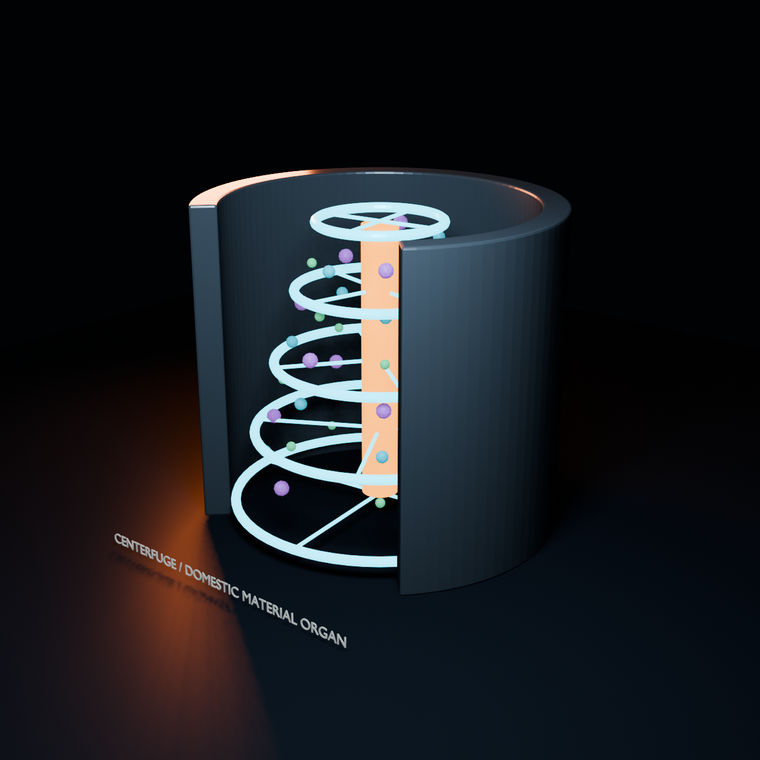
\includegraphics[width=0.52\textwidth]{figs/fig7_cutaway.png}
\caption{The cutaway render committed in the repository. The interior is plainly visible through the opening. The scene's own non-occlusion check, run as written under Blender $5.2.2$, reports a reached fraction of $0.34$ against a requirement of $0.6$.}
\end{figure}

\paragraph{The manifest check.} The script \texttt{check\_manifest.py} reads \texttt{manifest.json} and the directory listing, and it needs no Blender. It requires an entry for each of seven named scenes, the output files that the entry names, a recorded image verification for each rendered scene, and a recorded visibility verification for the two scenes that claim an interior view. This is a check on the completeness of a record: it establishes that the recorded steps were reported as having run and that the files they claim exist. It does not establish that a recorded verification was run on this code state, that its threshold is meaningful, or that the render shows what its label says. Run on the committed output directory it exits with failure, because that directory contains four scenes' files and no manifest. The separation of recording from admission, which the repository's own documents insist on, is respected in the code, and the value of the separation is exactly that the admitting step can be audited without trusting the recording one.

\begin{center}
\begin{tabular}{@{}p{0.26\textwidth}p{0.34\textwidth}p{0.32\textwidth}@{}}
\toprule
Check & A pass establishes & A pass leaves open\\
\midrule
Image non-degeneracy & The red channel of every seventh pixel varies by more than $1.5$ levels. & Any scene content; the other channels; correctness.\\
Non-occlusion & For up to $24$ sampled points per object, no other object lies on the segment from the camera. & Frame, facing, lighting, render flags, transparency; points on the object's own far side.\\
Manifest & A record exists and the files it names are present. & That the recorded checks ran on this code; that they are adequate.\\
\bottomrule
\end{tabular}
\end{center}

\section{A Check Built for the Question}

The arrangement scene of Section 7.3 performs a check designed for a stated purpose, and its structure is the one the suite's checks lack. The purpose is that a reader recover, for the visible vertices, the number of circles meeting there. The check therefore asks the image for exactly that: it detects regions of each class colour and compares their counts with two independent predictions from the scene, one a lower bound and one an upper estimate, and it reports the bracket and not a pass or fail. A conclusion drawn from it is correspondingly narrow. For the two arrangements and the one camera it establishes that colour recovers multiplicity of the visible vertices under Standard colour management; it says nothing about the other views, nothing about AgX, and nothing about the hidden vertices. The check also states a way to fail: a change of view transform moves the colours outside the detection tolerance, as the table of Section 7.4 shows.

The same pattern applies to quantities. The network run of Chapter 6 produced $121$ states of $54$ nodes, and Figure 7.3 shows three of them, at times $5$, $20$, and $120$, on three globes with a common orientation. Node colour comes from the viridis ramp applied to the stock divided by the largest stock in the whole run, $1.6869$, so the three globes are comparable and the early frames are dark by construction. That choice is deliberate: normalising each frame to its own peak would make every frame look equally saturated and would hide the growth that the sequence exists to show. Markers have a single size, so colour is the only carrier. The image was then read back. For each marker whose centre is reachable from the orthographic camera, the colour at the projected centre was matched to the nearest of the $256$ ramp colours and converted to a stock. Of the $162$ markers, $90$ are reachable by the centre ray, and $63$ of those face the camera by more than a cosine of $0.2$. For those $63$ the recovered stock is within $0.183\%$ of the peak, with a median error of $0.099\%$, which is the quantisation of a $256$-step ramp. The remaining $27$ grazing markers contain $5$ misreadings of between $4\%$ and $19\%$ of the peak. These are nodes at the limb for which the ray reports the marker as reached while the pixel at its projected centre shows a tube or the background, because most of the marker lies behind the globe. The centre-ray rule that the suite uses is therefore also not sufficient for legibility at grazing angles, and the readback is the check that detects it.

\begin{figure}[ht]
\centering
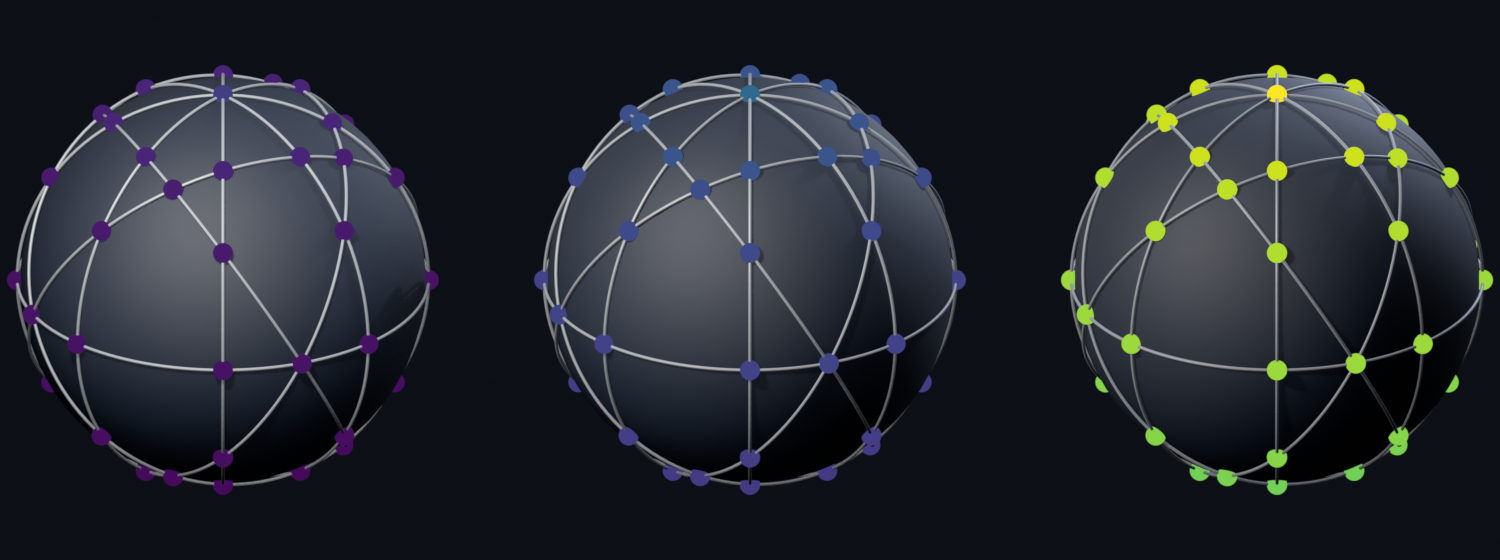
\includegraphics[width=\textwidth]{figs/fig7_network.png}
\caption{The network of Chapter 6 at times $5$, $20$, and $120$, with node colour from stock on a single ramp normalised by the peak stock of the whole run. Stock enters at the north pole, which becomes the brightest node, and spreads over the sphere. The ramp clamps stock below zero to its lowest colour, so a negative stock would be indistinguishable from zero in this image.}
\end{figure}

Two limits of the picture should be stated beside it. The ramp clamps negative stock to the bottom colour, as the Chapter 6 export script clamps negative scale, so a run that violated nonnegativity would look the same as one that did not, and the nonnegativity check of Chapter 6 must be made on the data. And a view shows about half of the nodes: $90$ of $162$ markers are reachable, and the south pole, where the drain acts, is on the hidden side in the chosen view. An animation of this kind is a presentation of a recorded run, and what it can support is a statement about visible nodes at the sampled times, resolved to the ramp's quantisation, for non-grazing nodes.

\section{Reading a Rendering Honestly}

The constructions of this chapter converge on a practice. State what the picture is meant to carry, choose a carrier suited to it, and measure that the carrier survives the chain from assignment to pixel. Colour needs a palette matched to the kind of information, an exposure and view transform that do not alter it, and a measurement of what the transform does. Shading needs a lighting model whose parameters are known, and the law $\rho P\cos\theta/(4\pi^2d^2)$ is that model for a point light in this renderer. A check on the result needs a stated purpose, and a passing check must be read for what it establishes. Ray-cast reachability, a red-channel contrast threshold, and a manifest of recorded results are each useful, and none of them is a judgment that the image is legible.

\begin{exercise}[7.1: Moving the colours]
Render the script's arrangement with the view transform set to AgX and run the colour detection with the tolerance of $22$ used in the text. State which classes are lost and by how much each channel moved. Then widen the tolerance until all three classes are recovered and check whether any two class colours can now be confused with each other or with the lit tubes. Finally choose a different measurement for the same purpose, for example a render with a flat unlit shader for the markers, and compare what each approach can and cannot say about the finished, tone-mapped image.
\end{exercise}

\begin{exercise}[7.2: A check that fits the cutaway]
Using the probe results above, design a replacement for the non-occlusion check that would accept the committed cutaway and reject an opaque shell. Decide which points to sample on curves and on the object's own surface, whether to require the points to be inside the frame, and whether the threshold should apply to each object or to the scene. Run the existing scene against your check and against the original, and write two sentences stating what your check establishes that the original does not, and what it still leaves open.
\end{exercise}

\begin{exercise}[7.3: Fitting the light]
Reproduce the table of Section 7.5 for an area light instead of a point light, varying power and distance. State the exponent you measure for distance and explain, by considering the geometry of the light's size, why it may differ from $-2$ at short range. Report the constant that replaces $1/(4\pi^2)$ for your light.
\end{exercise}

\chapter{Cameras, Shader Graphs, and Rendering Budgets}

\section{A Camera Is a Map}

Chapter 7 ended with a limit: a statement such as \emph{the arrangement has six quadruple points} is a statement about a model, and no single image certifies it. This chapter asks what a camera does to a model, how a shader graph can attach data to what the camera sees, and what an image costs. As in Chapter 7 the measurements were made with Blender's Python module, version $5.2.2$, run headless with the Eevee engine under software rendering, and the scripts named in the text are part of the evidence.

A perspective camera is a map from points of space to points of a rectangle. With the camera at the origin looking down its own negative $Z$ axis, a point with camera coordinates $(x,y,z)$, $z<0$, lands on the sensor at
\[
  u = f\,\frac{x}{-z},\qquad v = f\,\frac{y}{-z},
\]
where $f$ is the focal length in millimetres, and the sensor coordinates are converted to pixels by the number of pixels per millimetre. Blender's default sensor fit applies the sensor width, $36$ mm, to the longer side of the frame, so for a frame $W\times H$ with $W\ge H$ the scale is $W/36$ pixels per millimetre, and for a portrait frame the same sensor width is applied to $H$. The horizontal field of view of a landscape frame is $2\arctan\bigl(36/(2f)\bigr)$, which is $73.74^\circ$ at $24$ mm, $39.60^\circ$ at $50$ mm, and $23.91^\circ$ at $85$ mm. An orthographic camera drops the division by depth: points are projected along the view axis and scaled by a single orthographic scale, which is the width of the visible region in scene units. The depth division is the whole difference. Under it, two equal spheres at different distances appear at different sizes, and under the orthographic map they appear at the same size.

\lstinputlisting[language=Python,basicstyle=\ttfamily\footnotesize,breaklines=true,frame=single,columns=fullflexible,keepspaces=true,firstline=14,lastline=22]{camera_probe.py}

The formula is testable against rendered pixels. The script \texttt{camera\_probe.py} places five small emissive spheres at known points, renders a $400\times300$ frame with the world black, locates each sphere's centroid by connected-component analysis, and compares that with three predictions: the function above, Blender's own \texttt{world\_to\_camera\_view}, and the centroid after adding half a pixel for the pixel-centre convention. At $24$, $50$, and $85$ mm the largest distance between a predicted position and a measured centroid was $0.12$, $0.06$, and $0.06$ pixels, and the function above agreed with \texttt{world\_to\_camera\_view} to better than $10^{-4}$ pixel. The orthographic camera agreed with its prediction to $0.08$ pixel, and a $300\times400$ portrait frame, in which the sensor width governs the vertical side, agreed to $0.06$ pixel. The tests show that the textbook formula is the camera Blender implements, including the half-pixel convention and the sensor-fit rule, and a reader who needs to place an annotation, a label, or a measurement in an image can compute its position rather than reading it off by eye.

\section{What One View Can Certify}

An orthographic view of a sphere shows the points of its near hemisphere. For a vertex on the unit sphere with outward direction $\mathbf v$ and a view direction $\mathbf d$ pointing from the sphere toward the camera, the vertex is on the near side exactly when $\mathbf v\cdot\mathbf d>0$, and the number $\mathbf v\cdot\mathbf d$, the cosine of the angle between the two, is the \emph{facing}. A vertex near the limb has small facing and is foreshortened, so its marker is an ellipse seen edge-on and is easily hidden by a tube, as the readback of Chapter 7 found.

The vertex sets of the two arrangements of Chapter 11 are centrally symmetric. Every circle is a great circle, so if $\mathbf v$ lies on a set of circles then $-\mathbf v$ lies on the same set. It follows that for any direction $\mathbf d$ that is not perpendicular to a vertex, exactly half the vertices face the camera, and the measurement agrees: with $4000$ view directions spread evenly over the sphere, the script's arrangement showed $13$ of its $26$ vertices in every view and the teaching arrangement showed $27$ of $54$. The orthographic image is therefore blind to exactly half of the vertices at every moment, and a count of coloured markers in one image bounds the count for the model by a factor of two at best.

Two views from opposite sides see every vertex once. The practical question is how much margin they leave. Taking the facing of $0.2$ used in Chapter 7 as the threshold below which a marker is unreliable, the number of vertices above threshold in a single view varied from $8$ to $13$ (median $10$) for the script's arrangement and from $18$ to $26$ (median $22$) for the teaching arrangement. For an antipodal pair, the search over $4000$ directions found nine directions at which every vertex of the script's arrangement has $|\mathbf v\cdot\mathbf d|>0.2$, and none for the teaching arrangement, whose best pair leaves a smallest facing of $0.157$. A third view cures this: a greedy selection showed that three views suffice for both arrangements at the threshold $0.2$. The result is a design rule with a number attached, and it depends on the arrangement, because the teaching arrangement has more vertices to place away from a limb.

The geometric prediction was then compared with the ray-cast of Chapter 7, which includes the globe and the tubes. At the best antipodal direction, the surface bound found every vertex of the script's arrangement reachable in the two views, $13+13=26$, and every vertex of the teaching arrangement, $27+27=54$. The stricter centre bound, which asks for an unobstructed ray to the marker centre, certified $10+10=20$ and $19+19=38$. The gap between the bounds is the same phenomenon as in Chapter 7: markers seen obliquely can be partly covered by neighbouring tubes. Figure 8.1 shows the antipodal pair for the script's arrangement. In both images the markers are emissive and keep their assigned colours, but the surface and tubes in the left image are lit weakly because the two lights are fixed in the world, not attached to the camera. The lesson for a figure that will be compared across views is to fix the lights relative to the camera, or to accept that shading will differ between views and not to rely on it as data.

\begin{figure}[ht]
\centering

\includegraphics[width=0.48\textwidth]{figs/fig8_view_a.png}\hfill

\includegraphics[width=0.48\textwidth]{figs/fig8_view_b.png}
\caption{An antipodal pair of orthographic views of the script's arrangement, chosen to maximise the smallest facing ($0.214$). Together they show all $26$ vertices; either alone shows $13$. The left view looks at the side the key light misses, so the globe is dark while the emissive markers keep their colours.}
\end{figure}

\section{A Shader Graph Is a Function}

A shader node graph is a small program with the same structure as the construction functions of Chapter 6: nodes are functions, links are composition, and the output node fixes what is returned to the renderer. The arrangement scene of Chapter 7 used three materials, one per multiplicity class, each a two-node graph with a constant colour. The same result can be obtained from one material whose colour is computed from data stored on the object. The Attribute node, with type Object and the name of a custom property, reads that property for the object being shaded and returns it as a number. A Map Range node rescales it, a Color Ramp with constant interpolation turns three levels into three colours, and the Emission shader outputs the result.

\Needspace{22\baselineskip}
\lstinputlisting[language=Python,basicstyle=\ttfamily\footnotesize,breaklines=true,frame=single,columns=fullflexible,keepspaces=true,firstline=89,lastline=104]{view_budget.py}

The single material has five nodes and four links. It was applied to every marker of the script's arrangement in place of the three class materials, and the scene was rendered twice at $450$ px and $16$ samples. Both renders contained the same connected regions of each class colour, $(8,5,3)$ for multiplicities $2$, $3$, $4$, and no pixel of the two images differed by more than two levels out of $255$, among $202{,}500$ pixels. The graph therefore reproduces the three-material result exactly in this scene. What it changes is where the information lives. In the three-material scene the class is stored twice, as a custom property and as a choice of material, and the two can disagree if one is edited. In the one-material scene the colour is a function of the property, so editing the property changes the colour, and a different arrangement needs only different property values. The cost is that the mapping from numbers to colours is hidden in the graph, so the ramp stops belong in the same record as the parameters, as Chapter 5 asks for modifier orders.

Two cautions follow from the measurement. First, the check shows that the graph matches the earlier material under Standard view transform and emission strength one; under another view transform both would change together, as Chapter 7 showed. Second, replacing the materials left the old three in the file as unused datablocks, so the scene file had six materials when only one was in use. This is the accumulation of Chapter 6 again, and the purge there applies.

\section{What a Render Costs}

A rendered image is the average of many samples per pixel, and the number of samples is a setting. Eevee's default for final renders is $64$. The effect of the setting on the result was measured on the script's arrangement at $300\times300$ pixels, taking a $256$-sample render as reference and reporting the root-mean-square difference over all pixels and channels, in levels out of $255$.

\begin{center}
\begin{tabular}{rrrr}
\toprule
Samples & RMS difference & Largest difference & Time (s)\\
\midrule
1 & 20.19 & 224 & 4\\
4 & 4.73 & 86 & 7\\
16 & 1.90 & 46 & 14\\
64 & 0.76 & 13 & 48\\
256 & (reference) & (reference) & 191\\
\bottomrule
\end{tabular}
\end{center}

Each fourfold increase in samples from $4$ to $64$ divided the RMS difference by about $2.5$, which is steeper than the factor of two that independent noise alone would give. The reference is itself a finite render, so the figures understate the true error, and the factor should not be read as a law. The largest single-pixel difference shows why an average hides what matters: at $16$ samples some pixel is still $46$ levels off, which is enough to move a marker's colour to another class on an eight-bit scale. The times for one and four samples come from the first measurement run and the others from a second run after a warm-up render, so the table is a rough guide; timings in this environment are specific to a software-rendered, windowless build, and they show a pattern more than a rate. Time grew about linearly with samples. It grew weakly with pixels: at $16$ samples, $300$, $600$, and $900$ pixels square took $14$, $18$, and $25$ seconds, so most of the cost of a small render was fixed per frame. A reader's machine will give different numbers, and the budget that matters is the one measured on the machine that will produce the final images.

Eevee proved deterministic in this configuration, on the evidence of two renders of the same scene with the same settings that were bit-identical, so a difference between two images could be attributed to a difference in the scene or in the settings and not to chance. Two renders are weak evidence, and Chapter 24 later found scenes in this same environment, with several hundred objects reading a material attribute at four samples, in which repeated renders of an unchanged scene were not identical. The property should therefore be checked, by repeated renders and a comparison of pixels, for each scene whose images are to be compared, and it is not guaranteed across hardware or Blender versions.

\section{Recording a Render}

The render budget is only comparable if the settings that produced an image are written down. The script below collects the settings that the measurements of this chapter and the last showed to matter: the Blender version, engine, resolution and resolution percentage, samples, view transform, look and exposure, the camera's type, focal length, sensor, orthographic scale, location and rotation, and the type and power of each light. It returns a dictionary that can be saved beside the image, and a short digest of the dictionary gives a quick equality test.

\Needspace{22\baselineskip}
\lstinputlisting[language=Python,basicstyle=\ttfamily\footnotesize,breaklines=true,frame=single,columns=fullflexible,keepspaces=true,firstline=8,lastline=26]{render_record.py}

On the script's arrangement the digest was \texttt{a55f051f3e2e}; setting the sample count to $16$ changed it to \texttt{17d9b2e75d7a}, and a second reading of an unchanged scene reproduced it. The record does not capture everything. It omits material parameters, mesh content, world colour, and the Python script itself, and a complete record would add the hash of the scene file and the commit of the construction script. It is the minimum that lets a reader say whether two renders were made under the same viewing conditions.

\section{What Was and Was Not Measured}

The measurements of this chapter establish that the pinhole formula and the field-of-view relation hold for the installed build, that half of the vertices of a centrally symmetric arrangement are hidden in every orthographic view, that three views reach every vertex of both arrangements at facing $0.2$, that one data-driven material reproduces three assigned materials in this scene, and that the sample count trades error against time in the measured way. They do not establish anything about Cycles, which was not available, about hardware-accelerated rendering, about lenses with distortion or depth of field, or about the interactive viewport. The camera comparison used point-like sources, so it says nothing about how well a thin line or a bevelled edge is localised. The sample study used a single scene and a single resolution.

\begin{exercise}[8.1: Fix the lights to the camera]
Parent the two lights of the arrangement scene to the camera and rerender the antipodal pair of Figure 8.1. Measure the mean brightness of the globe in the two views before and after, and state which change in the figure you would attribute to the lights and which to the geometry.
\end{exercise}

\begin{exercise}[8.2: A third view]
For the teaching arrangement, find a direction $\mathbf d_3$ that, added to the best antipodal pair, makes every vertex have facing above $0.2$ in at least one of the three views. Verify with a ray-cast in Blender that the centre bound then certifies as many of the $54$ markers as it can, and report the number.
\end{exercise}

\begin{exercise}[8.3: Edit the property, not the material]
Change the \texttt{multiplicity} property of one marker in the one-material scene and rerender. Confirm that its colour changed and that no material was edited. Then add a fourth class to the ramp, and write the sentence that a figure caption must contain so that a reader can recover the mapping.
\end{exercise}

\begin{exercise}[8.4: A budget for a figure]
Choose the smallest sample count at which the largest single-pixel difference from a $256$-sample reference is below $13$ levels for your own scene, and record the settings with the script of Section 8.5. State the machine on which the time was measured.
\end{exercise}

\chapter{Representational Adequacy: One Geometry, Four Presentations}

\section{Adequacy Made Measurable}

Chapter 7 asked what a picture of a structure can carry, and Chapter 8 asked what a camera does to it. This chapter fixes a single geometry and changes only how it is presented. The development plan of this book states the governing idea as an inequality. Given a full state $x$, a reduced representation $r(x)$, and a question $Q$, a procedure $\widehat Q$ that answers the question from the reduced representation is adequate to the extent that
\[
  d\bigl(Q(x),\,\widehat Q(r(x))\bigr)\le\varepsilon
\]
over a stated domain of states. Here the state $x$ is the geometry of the habitat of Chapter 3, the representation $r$ is a presentation (a plan, an eye-level view, a cutaway, a wireframe), the question $Q$ is a property of the geometry that someone might want to know, and $\widehat Q$ is whatever a reader, or a script standing in for a reader, does with the image. The same presentation can be adequate for one question and badly wrong for another, so no presentation is good in itself, and a statement about a presentation has the form: for this question, on this geometry, with this reading procedure, the error is this large.

The plan is to make the left side of the inequality computable in a few cases, so that the habit of asking the question has numbers to attach to it. Two cautions apply. A reading procedure must be specified before the error can be measured, and a human reader's procedure is not fully specified, so the procedures used here are simple automatic ones whose failures are informative but not exhaustive. And $\varepsilon$ comes from the purpose of the work, not from the measurement: whether an error of $8$ percentage points in a visible-floor fraction matters depends on what the fraction will be used for.

\section{The Habitat as Data}

The habitat of Chapter 3 was built by hand from dimensions in the text. To measure anything about it, the same construction is needed as data. The script below builds it in a collection named \texttt{Habitat}, with the platform top at $z=0$, the north wall $6$ long, the east and west walls $5.6$ long between the inner faces of the north and south boundaries, a south wall in two blocks that leave a gap, and a low plinth. There is no roof. Two entrance variants stand for the two saved files of Exercise 3.4: a gap of width $1.2$ centred on the south wall, and a gap of the same width at the east end, $x\in[1.6,2.8]$. The plinth is $0.8\times0.8\times0.5$ at $(-1,1)$ in both.

\Needspace{26\baselineskip}
\lstinputlisting[language=Python,basicstyle=\ttfamily\footnotesize,breaklines=true,frame=single,columns=fullflexible,keepspaces=true,firstline=12,lastline=45]{habitat.py}

The script was run in Blender 5.2.2 and its check function read the built objects back. Each variant has seven objects; the platform top is at $z=0.000$; every wall spans $z=0$ to $2.5$; the south gap measures $1.200$ in both variants; the east wall lies between $x=2.8$ and $3.0$ and has length $5.60$; and the inner faces of the north and south walls are at $y=2.80$ and $y=-2.80$, where the ends of the east and west walls stop. The construction is therefore the one the chapter describes, and the numbers below refer to it.

\section{Two Questions}

Two questions about this geometry are used throughout. Question A concerns an observer and has the form of Exercise 3.4: what fraction of the interior floor can a person standing in the doorway, with eyes at height $1.6$, see? Question B concerns the structure: where is the entrance?

The answer to A is defined by ray-casting. The interior floor, $5.6\times5.6$, is divided into $56\times56$ cells of side $0.1$. A cell counts as reachable if the straight segment from the eye, placed in the plane of the south wall at the centre of the gap, to the cell centre meets no object. For the centred entrance $2806$ of $3136$ cells are reachable, $89.5$ percent. For the east entrance $2646$ are reachable, $84.4$ percent. The two variants differ by five percentage points. Two things are expected to contribute, the thickness of the wall beside the doorway, which hides a strip of floor along the south wall, and the position of the observer, who stands near a corner in the second variant; the contribution of each was not separated here. The plinth hides a shadow-shaped region behind it in both. The truth for B is the gap, $[-0.6,0.6]$ or $[1.6,2.8]$.

\section{Four Presentations}

Figure 9.1 shows the east-entrance habitat in four presentations: a plan, an eye-level view from the doorway, a cutaway, and a wireframe. The geometry is identical in all four and the lighting is ambient only, so no cast shadow decides what a panel appears to show.

\begin{figure}[ht]
\centering
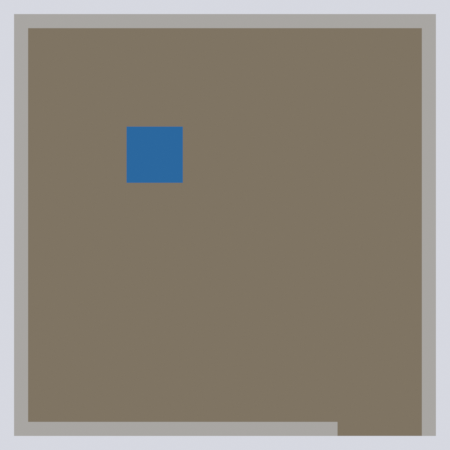
\includegraphics[width=0.48\textwidth]{figs/fig9_plan.png}\hfill
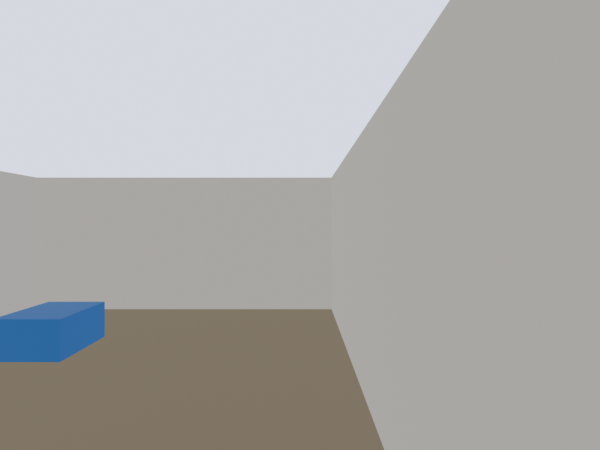
\includegraphics[width=0.48\textwidth]{figs/fig9_eye.png}\\[4pt]
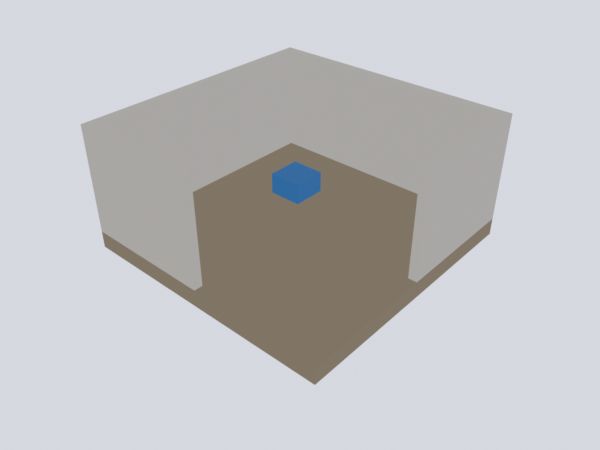
\includegraphics[width=0.48\textwidth]{figs/fig9_cut.png}\hfill
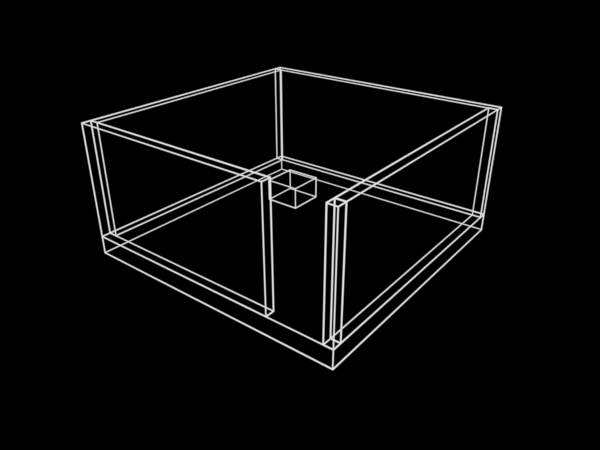
\includegraphics[width=0.48\textwidth]{figs/fig9_wire.png}
\caption{The east-entrance habitat. Top left, plan from above with an orthographic camera. Top right, eye-level view at $1.6$ from the doorway, $90^\circ$ horizontal field of view, looking north. Bottom left, a cutaway made with a Boolean difference that removes the south-east quadrant of the walls. Bottom right, the same geometry as a wireframe from the oblique camera used for the counts in the text.}
\end{figure}

\paragraph{Plan.} The plan answers Question B well. The wall tops, floor, and plinth top are flat colours, and reading the gap as the run of non-wall pixels along the south wall recovered its ends to within one pixel at every resolution tried.

\begin{center}
\begin{tabular}{rrrr}
\toprule
Size & mm per pixel & Error, centre & Error, east\\
\midrule
100 px & 64 & 24 mm & 16 mm\\
200 px & 32 & 8 mm & 16 mm\\
400 px & 16 & 8 mm & 0 mm\\
\bottomrule
\end{tabular}
\end{center}

The same plan answers Question A badly. Every point of the floor is visible from above except the footprint of the plinth, so the share of floor-coloured pixels in the interior, which is the only answer the plan can give, was $97.8$, $97.4$, and $97.96$ percent at the three resolutions, against a geometric value of $1-0.64/31.36=97.96$ percent. The plan reports $98$ percent where the truth is $89.5$ or $84.4$. The error is about $8.5$ points in one variant and $13.5$ in the other, and the plan reports the same number for the two entrances. The reason is structural: the plan is the view of an observer at infinity above the room, and Question A asks about an observer in a doorway. A plan that is accurate and well rendered is not adequate to the question.

\paragraph{Eye-level view.} The eye-level view is the observer's own sample, and it can be made to answer A by a rendering trick. The floor is given an emission colour that encodes its position, red proportional to $x$ and green to $y$, and everything else is black, with anti-aliasing off, a single sample, and a raw view transform so that the stored values are the assigned values. Each floor pixel then says which floor point it shows, and the cells that appear are the cells the image can speak about. The script \texttt{presentations.py} did this at $800\times600$ with a $90^\circ$ lens. For the centred entrance the image contained $1745$ distinct cells, and $1724$ of them were exactly the cells that the ray-cast found both reachable and inside the frame; for the east entrance the image held $1307$ cells, of which $1294$ matched. No cell that was reachable and in frame was missing from the image. The $21$ and $13$ extra cells are cells whose centres are hidden but whose edges are visible, which is the centre-versus-surface distinction of Chapter 7 in a different setting.

The eye-level view has a different limit. A $90^\circ$ frame cannot contain what is beside or behind the observer, and of the $2806$ and $2646$ reachable cells, $1082$ and $1352$ lay outside the frame. The image therefore speaks to $1724/2806=61$ percent of what the observer can see in the first variant and $1294/2646=49$ percent in the second. The fraction of the floor visible within the frame was $55.0$ and $41.3$ percent, and that number is a property of the camera's field of view as much as of the room. Question A as posed asks for the observer's visibility, and a single narrow-angle image underestimates it. A panoramic camera or several views turned in different directions would answer it, and the cost, as in Chapter 8, is a count of views.

\paragraph{Cutaway.} A cutaway shows interior arrangement by removing the near surfaces, and what it removes cannot be read from it. The cutter used here deletes the south-east quadrant of the walls, which contains the entrance of the east variant, so the cutaway shows the plinth and the north and west walls clearly and shows neither the entrance nor the walls that determine what the doorway observer sees. For Question A it cannot be used at all, since the walls that hide the floor from the doorway are among those removed. For Question B it answers wrongly in a particular way: the opening where the south wall has been cut away looks like an entrance of great width, and nothing in the image distinguishes the cut from the doorway. A cutaway is adequate for questions about what the removed surfaces were hiding, and a reader needs to be told what was removed.

\paragraph{Wireframe.} A wireframe preserves all the edges, hidden or not, and so keeps the geometry's incidence structure while discarding surfaces. What it adds is crossings that are not in the geometry. Using the oblique camera of the figure, with $84$ edges in the seven meshes, $82$ pairs of edges cross on the screen without meeting in space and $7$ cross where they also meet, for the centred entrance, and $62$ and $7$ for the east entrance. The false crossings are about ten times as many as the true ones. If only the edges whose midpoints are unobstructed are drawn, a crude stand-in for a solid view, the false crossings fall to $8$ and $3$ with $3$ true ones. From an elevation straight toward the south wall the wireframe has $74$ and $58$ false crossings and none true, because the edges of the near and far walls project onto each other. A reader looking at a wireframe has to decide, at each crossing, whether two edges meet, and the numbers say how often the picture offers that decision as a trap. The measure counts crossings of edges and does not count overlapping collinear edges, which also confuse a reader, so it understates the problem.

\section{What the Experiment Does Not Show}

The experiment used one geometry in two variants and one observer height, and the questions were chosen because they separate the presentations. Nothing here shows that a plan is a poor presentation in general or that a wireframe is poor; they answer different questions, and the reader who wants to know where the entrance is should consult the plan. The reading procedures were automatic: the cell-identity decoding is not how a person looks at a picture, and a person might use cues the procedure ignores, such as the convergence of lines to read depth in the eye-level view. The measurement of false wireframe crossings assumes that every crossing is a risk of misreading, which a practised reader may resolve at a glance. The distance used, an absolute difference in a fraction or a position, is one of many that could stand for $d$ in the adequacy inequality. And the tolerance $\varepsilon$ was never specified, because it is a matter of purpose. The purpose of the habitat in this book is to be revisited from several positions, which makes Question A the more relevant of the two, and makes the plan, despite its excellent recovery of the entrance, the least adequate presentation for it.

\section{Writing an Adequacy Statement}

A caption or a report that uses a presentation can state its adequacy compactly, in the form the inequality suggests. The statement names the geometry, the question, the presentation, the reading procedure, the distance, and the measured error. For the habitat it can read: \emph{for the east-entrance habitat, the question of what fraction of the floor is visible from the doorway at height $1.6$, read as the share of floor-coloured pixels in the plan, has an error of $13.5$ percentage points, so the plan is not used for it; read from a cell-identity render at $90^\circ$ field of view, the image covers $49$ percent of the reachable cells, so a single image underestimates visibility.} The sentence is longer than a caption usually is, and it can be shortened once the structure is understood. What must not be shortened away is the question, since the same image supports a different statement for each question.

\begin{exercise}[9.1: Move the observer]
Repeat Question A for an observer standing $1.0$ inside the room at the centre of the gap, and for an observer seated with eye height $1.1$. Report the reachable fraction for both entrance variants and describe which of the four presentations of Figure 9.1 changes its answer, and which does not.
\end{exercise}

\begin{exercise}[9.2: A cutaway that answers]
Choose a cutter that removes only the roofless wall above eye height $1.6$ on the east side and keeps the south wall intact. State one question that this cutaway answers and one that it does not, and test each with a reading procedure of your own.
\end{exercise}

\begin{exercise}[9.3: A panoramic answer]
Use a panoramic camera, or four views turned by $90^\circ$ about the vertical axis at the doorway, to answer Question A from images alone. Report the number of cells the images can speak to and compare it with the ray-cast truth. State the number of views and the field of view that reached at least $95$ percent of the reachable cells.
\end{exercise}

\begin{exercise}[9.4: Moving the plinth]
Move the plinth to the middle of the room and repeat the ray-cast truth for Question A. Predict beforehand whether the reachable fraction will rise or fall, state the geometric reason, and then measure.
\end{exercise}

\chapter{Surface Treatment, Ornament, and Essential Visibility}

\section{Ornament Is Relative to a Question}

A surface treatment is anything done to the appearance of geometry without changing the geometry: a colour, a texture, a bump pattern, a gloss, a shading model. Chapter 9 showed that a presentation is adequate or not relative to a question. The same holds for the treatments applied within a presentation. A feature of a surface is \emph{ornament relative to a question} when removing it changes the answer a reading procedure gives by no more than the tolerance $\varepsilon$ of Chapter 9, and it is \emph{essential} to that question when removing it changes the answer by more. The definition is operational. It can be tested by rendering the scene with and without the feature, applying the same reading procedure to both images, and comparing the answers. And it is relative: a wood grain on a floor is ornament for the question of where the entrance is and may be essential for the question of whether the floor is timber.

Ornament is not worthless, and the point of the definition is not to remove it. The point is to know what each treatment costs and what it buys, so that a figure carries the ornament its purpose can afford. A treatment can also cost something that is not decoration at all. A noise pattern has no information about the plinth, and it can still damage a reader's ability to find the plinth. This chapter measures that damage in a simple case, shows that its onset can be predicted from the colours alone, reports the cost in render time, which proved undetectable, and shows what a shading model contributes beyond colour.

\section{A Reading Task and a Noise Pattern}

The task is to find the plinth in an oblique view of the habitat of Chapter 9, with the east entrance. The reading procedure assigns each pixel to the nearest of four reference colours (plinth, floor, wall, background), measuring distance in the CIE Lab colour space, in which Euclidean distance approximates perceived colour difference. The distance between two colours in Lab is written $\Delta E$. The plinth is scored against a mask produced by rendering the same view with flat identity colours, and the score is the intersection over union of the pixels the procedure calls plinth with the pixels that are plinth. Precision is the share of called pixels that are right, and recall the share of true pixels that are called.

The ornament is a procedural noise pattern on the floor. A Noise Texture node, fed with object coordinates, is rescaled by a Map Range node and drives a Mix node between two tones of the floor colour, one darker and one lighter than the floor's base colour by a relative amplitude $a$. At $a=0$ the floor is flat, and at larger $a$ it is a speckle whose average tone stays at the base colour. The materials are emissive, so the pixel colours are the assigned colours, and the experiment isolates the effect of the pattern from the effect of lighting. The script is \texttt{ornament.py}.

Three plinth colours were used. The \emph{distinct} plinth is the blue of Chapter 7's palette, at $\Delta E=58.1$ from the floor's base colour. The other two are the floor colour scaled up in tone, by $1.15$ and by $1.45$, so that they have the same hue as the floor and differ in lightness only; their distances from the floor colour are $\Delta E=8.0$ and $23.8$. The tonal plinths are the hard case, because the noise pattern moves floor pixels along exactly the line that joins the floor colour to the plinth colour.

\section{What the Pattern Costs}

\begin{center}
\begin{tabular}{rrrr}
\toprule
Amplitude $a$ & sd of floor $L^*$ & IoU, $\Delta E=8.0$ & IoU, $\Delta E=23.8$\\
\midrule
0.00 & 0.00 & 1.000 & 1.000\\
0.10 & 2.14 & 0.447 & 1.000\\
0.20 & 4.22 & 0.123 & 1.000\\
0.35 & 7.15 & 0.073 & 0.249\\
0.50 & 8.10 & 0.060 & 0.106\\
\bottomrule
\end{tabular}
\end{center}

The blue plinth at $\Delta E=58.1$ was found with an intersection over union of $1.000$ at every amplitude, so for it the pattern is ornament in the sense defined above. For the two tonal plinths the pattern is not ornament: it takes the score from $1.000$ to $0.447$ at $a=0.10$ for the closer colour, and from $1.000$ to $0.249$ at $a=0.35$ for the other. In every case recall stayed at $1.000$ and precision equalled the score. The reading procedure never missed the plinth, because the plinth's colour was exact, and the entire loss came from floor pixels that the noise made closer to the plinth colour than to the floor colour. Figure 10.1 shows the case $\Delta E=23.8$ at three amplitudes, with the reading below each image.

\begin{figure}[ht]
\centering
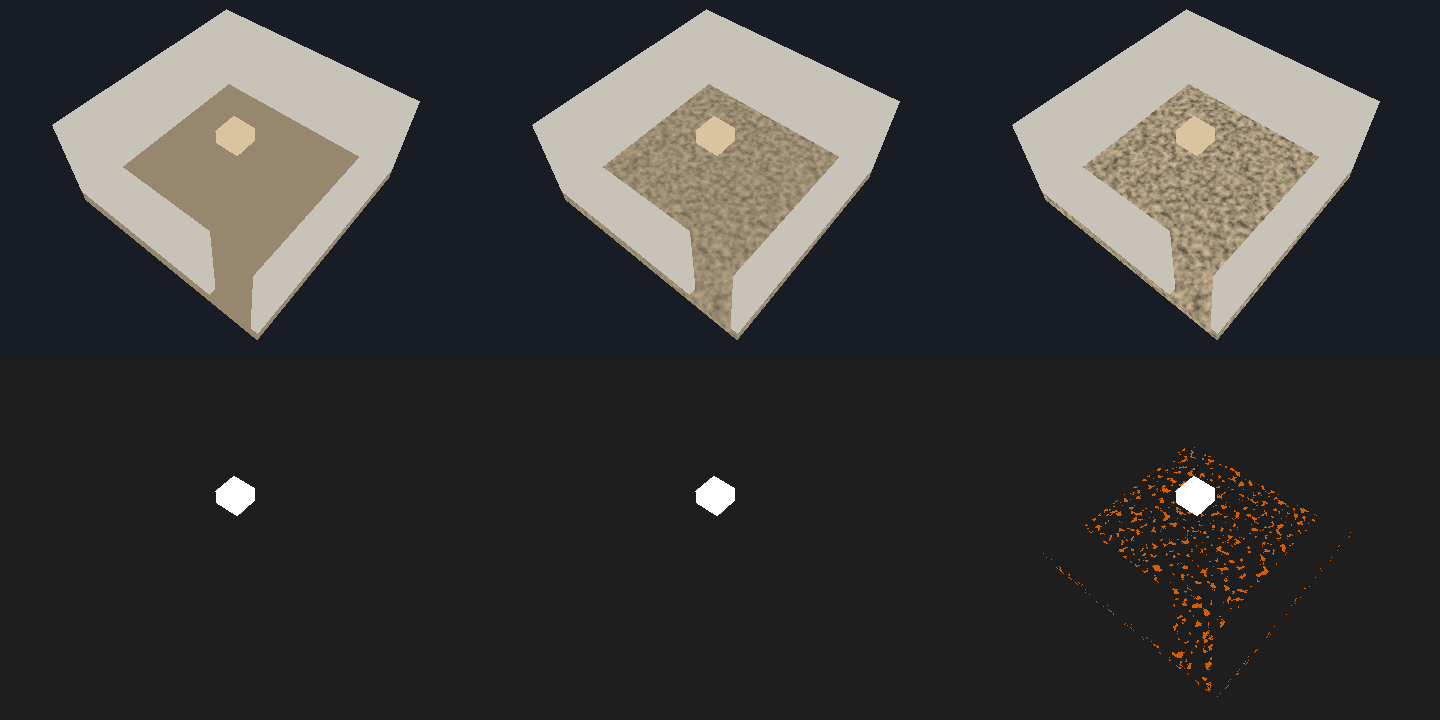
\includegraphics[width=\textwidth]{figs/fig10_ornament.png}
\caption{A plinth $1.45$ times the floor colour under floor ornament of amplitude $0$, $0.2$, and $0.35$ (top, left to right), and the nearest-colour reading of each (bottom). White marks plinth pixels found and orange marks floor pixels wrongly called plinth. At $a=0.2$ the reading is still exact, and at $a=0.35$ about three quarters of the pixels it calls plinth are floor.}
\end{figure}

The onset is predictable from the colours. The pattern moves a floor pixel as far as $a$ times its colour toward the plinth, and the reading procedure calls a floor pixel plinth when it has moved past the midpoint of the two colours. If the plinth is the floor colour multiplied by $s$, the midpoint is at $1+(s-1)/2$, and errors can begin when $a$ exceeds about $(s-1)/2$. For $s=1.15$ this is $0.075$ and the first failure was at $a=0.10$, the smallest amplitude tried above zero. For $s=1.45$ it is $0.225$, and the score was still $1.000$ at $0.20$ and had fallen at $0.35$. The rule is a first estimate: it works in sRGB scaling while the reading works in Lab, the pattern's extreme tones are reached only where the noise saturates, and the share of pixels beyond the midpoint depends on the pattern's distribution, so the rule says where errors begin and not how many there are. It is nevertheless the form of the useful statement, which is a relation between the spread of the ornament and the separation of the colours that carry the information.

The finding is specific to the reading procedure. A procedure that used shape, such as requiring a connected region of roughly the plinth's size, would tolerate much more noise, and a human reader's performance is unlikely to collapse as abruptly as a nearest-colour classifier. The measurement shows what a plain colour classifier needs, and a reader or a script that has a better procedure has less need of colour separation. Colour separation is cheap to provide and does not depend on the reader's skill, which is a reason to keep it when the figure must be read by an unknown reader.

\section{What the Pattern Costs in Time}

Chapter 8 measured render cost against samples and pixels, and it is natural to ask whether the pattern adds to it. A flat floor and a noise floor of amplitude $0.35$ were each rendered three times at $960\times720$ and $16$ samples, after a warm-up. The flat floor took $5.4$, $11.3$, and $10.8$ seconds and the noise floor $4.3$, $10.7$, and $10.9$ seconds. The runs with identical settings differed by a factor of two, so any difference attributable to the pattern is far below the scatter of the measurement, and no cost was detected. The pattern is a few nodes evaluated per pixel, and in this software-rendered configuration the fixed per-frame cost of Chapter 8 dominates. The conclusion is limited to this configuration and this scale. It does not say that textures are free on a graphics card with a large image, or in an animation of many frames, where a small per-pixel cost multiplies.

\section{What a Shading Model Adds}

The flat emissive materials used above erase one thing the plinth has, which is its form. In the flat render the plinth's mask contains a single colour, one distinct value in $1042$ pixels, with $L^*=46.0$, so the box looks like a hexagon. Rendered again with diffuse materials under ambient light and one sun lamp, the same mask contained six distinct colours of which three had at least twenty pixels, at $L^*=29.6$, $36.1$, and $36.2$. A shading model therefore separates the top of the plinth from its sides by $6.5$ units of $L^*$ and does not separate the two visible sides from each other, which differ by $0.1$. For the question of where the plinth is, the shading is ornament, because the reading above found it with a score of $1.000$ either way. For the question of whether the object is a solid box, the shading is essential, because without it the image contains nothing that says so. The two sides that are indistinguishable show a further point: a shading model gives information only where the light makes surfaces differ, and a light placed so that two faces receive the same illumination is a light that discards the distinction between them.

\section{A Rule for Choosing}

The measurements suggest a procedure for deciding how much surface treatment a figure should carry. List the questions the figure is meant to answer, and for each, write the colour or tone difference that carries its answer. Keep the separation between those colours larger than the spread of any ornament that will share their region of the image, using a relation such as $a<(s-1)/2$ as a first estimate and a rendered test as a confirmation. Then test whether each treatment is ornament or essential by removing it and applying the reading procedure, and keep the essential ones. What remains is a figure whose ornament was chosen, and whose cost is known to be small for the questions asked, and whose omission would not have changed what the reader can recover. The costs that were found are on the reader's side and not the renderer's, and that is why they deserve a measurement and not an assumption.

\begin{exercise}[10.1: Move the threshold]
Choose a plinth colour with $s=1.30$ and predict the amplitude at which the nearest-colour reading begins to fail, using $(s-1)/2$. Then measure the score at amplitudes $0.05$ to $0.30$ in steps of $0.05$ and report how close the prediction was.
\end{exercise}

\begin{exercise}[10.2: A better reader]
Add a second reading procedure that requires a candidate region to be connected and to contain between $500$ and $2000$ pixels, and repeat the measurement for the plinth with $\Delta E=8.0$. State the amplitude at which the new procedure fails, and say what it assumes about the plinth that the nearest-colour procedure did not.
\end{exercise}

\begin{exercise}[10.3: Ornament for a different question]
Choose a question for which a floor pattern is essential, such as whether the floor is made of a material with visible grain, and write a reading procedure and an ablation test for it. Show that the pattern is ornament for the plinth question and essential for yours.
\end{exercise}

\begin{exercise}[10.4: Lights that merge faces]
Find a direction for the sun lamp at which the top and sides of the plinth have the same $L^*$ to within $0.5$, and report what the image of the plinth then shows. State the lesson for a figure that must show form.
\end{exercise}


\setcounter{part}{3}
\part{First Mathematical Construction: The Nine-Orthodrome Workshop}

\begin{checkpoint}[Numbering]
Chapters 8 through 10 (shader nodes, cameras, and rendering) are planned in the development plan and not yet written. The chapter below keeps its planned number, 11, so that cross-references to the plan remain stable.
\end{checkpoint}

\setcounter{chapter}{10}
\chapter{From Plane Normals to a Spherical Network}

\section{Source and Scope}

This chapter derives its source construction from \emph{Orthodromic Infrastructure Blueprint}, Chapter 3, Sections 3.1 to 3.6, printed pages 13 to 20. Section 3.6 specifies an equator and four polar reference circles, followed by four configurable inclined circles. The worked coordinates below instantiate that family for teaching. They do not resolve the blueprint's question of symmetry versus planetary fit. The corridor definitions of the blueprint's Chapter 2 and the service geometry of its Chapter 4 supply further distinctions introduced here.

The task is to construct nine curves on a common sphere, preserve their mathematical identities, and inspect their intersection graph. This is a geometric model. Its successful construction does not establish the engineering adequacy of a planet-scale infrastructure system.

\section{A Circle as a Plane-Sphere Intersection}

For radius $R>0$ and a unit vector $\mathbf n$, define
\[
  S_R^2=\{\mathbf x\in\mathbb R^3:\|\mathbf x\|=R\},\qquad
  O(\mathbf n)=\{\mathbf x\in S_R^2:\mathbf n\cdot\mathbf x=0\}.
\]
The plane passes through the sphere's centre, so its intersection is a great circle. Multiplying the normal by a nonzero scalar leaves the plane unchanged; requiring unit length removes the magnitude ambiguity but leaves $O(\mathbf n)=O(-\mathbf n)$. The space of unoriented plane normals is consequently the real projective plane. A circle's identity must not be inferred from the sign of its normal.

To draw the circle, choose perpendicular unit vectors $\mathbf u$ and $\mathbf v$ spanning its plane. Then
\[
  \mathbf x(t)=R(\mathbf u\cos t+\mathbf v\sin t),\qquad 0\le t<2\pi.
\]
Since $\mathbf n$ is perpendicular to $\mathbf u$ and $\mathbf v$, $\mathbf n\cdot\mathbf x(t)=0$. Since $\mathbf u$ and $\mathbf v$ are orthonormal, $\|\mathbf x(t)\|^2=R^2(\cos^2t+\sin^2t)=R^2$. These calculations establish that every sampled point lies on the intended circle. They are also useful numerical checks.

Choose a reference vector $\mathbf a$ that is not nearly parallel to $\mathbf n$, and set
\[
  \mathbf u=\frac{\mathbf a\times\mathbf n}{\|\mathbf a\times\mathbf n\|},\qquad
  \mathbf v=\mathbf n\times\mathbf u.
\]
Near-parallel vectors make the denominator small, so an implementation must choose a different reference axis in that case. The basis is a drawing convention; rotating $\mathbf u$ and $\mathbf v$ within the plane changes the starting parameter but not the circle.

\section{The Fixed Five}

Take $\mathbf n_E=(0,0,1)$. Choose a reference azimuth $\lambda_0$ and define
\[
  \mathbf n_{P,k}=\bigl(\cos(\lambda_0+k\pi/4),\ \sin(\lambda_0+k\pi/4),\ 0\bigr),
  \qquad k=0,1,2,3.
\]
All four polar planes contain the $Z$ axis. They therefore share the north and south poles. Their normals occupy four distinct directions over a half-turn, because a normal's antipode denotes the same plane. A spacing of $\pi/2$ would repeat planes instead of providing four distinct polar circles.

The normal's azimuth is not the longitude of the circle's equatorial intersection. For a horizontal normal of azimuth $\lambda$, the equatorial intersection directions have azimuth $\lambda\pm\pi/2$. This distinction prevents a ninety-degree error when using geographic labels.

For $q$ polar circles plus one equator, the blueprint derives $V=2+2q$, $E=6q$, and $F=4q$. With $q=4$, $V=10$, $E=24$, $F=16$. The two polar intersections are each single vertices of multiplicity four. Counting pairwise circle intersections without merging coincident positions would give an incorrect graph.

\section{The Configurable Four}

The source permits normals
\[
  \mathbf n_i=(\cos\beta_i\cos\lambda_i,\ \cos\beta_i\sin\lambda_i,\ \sin\beta_i),
  \qquad i=6,7,8,9.
\]
Here $\beta$ is the latitude of the normal, or pole of the great circle, not the circle's tilt relative to the equatorial plane. The unoriented angle between that plane and the equatorial plane is $\arccos(|\sin\beta|)$. Calling $\beta$ simply ``inclination'' can therefore mislead readers.

For the teaching example choose $\lambda_0=0$, $\beta=\pi/6$, and seed azimuth $\alpha=\pi/8$. Generate four normals using $R_z(\pi/2)$:
\[
  R_z(\theta)=\begin{pmatrix}
    \cos\theta&-\sin\theta&0\\
    \sin\theta&\cos\theta&0\\
    0&0&1
  \end{pmatrix},\qquad
  \mathbf n_{F,k}=R_z(k\pi/2)
  \begin{pmatrix}\cos\beta\cos\alpha\\ \cos\beta\sin\alpha\\ \sin\beta\end{pmatrix}.
\]
The nonzero seed azimuth is an explicit revision of an earlier provisional $\alpha=0$ example. It moves the equatorial intersections away from the polar family's equatorial vertices. Symmetry still produces other multiway intersections, so this is not a general-position arrangement. The choice of rotation, $\beta$, and $\alpha$ is a teaching example within the family the blueprint describes, and is not an additional specification attributed to the source.

The parameter variation exposes structure. At $\beta=0$, the four flexible normals repeat two polar planes up to sign. At $|\beta|=\pi/2$, they all represent the equator. More generally, $R^4=I$ guarantees orbit closure but does not guarantee four distinct projective normals. Test distinctness with $|\mathbf n_i\cdot\mathbf n_j|$ near one, rather than testing only whether $\mathbf n_i$ and $\mathbf n_j$ are equal.

\section{The Blender Construction Through the Interface}

On a separate saved scene, add a curve circle through \texttt{Add > Curve > Circle}. Set its location to the origin and its rotation to zero. The primitive's default plane is the local $XY$ plane, with normal along local $Z$. Inspect its dimensions and scale it to the desired radius. Use a thin bevel only to make the curve visible as a corridor centreline representation. A built-in curve circle is a convenient visual construction; it should not replace analytic coordinates when numerical accuracy is being evaluated.

Duplicate the circle for each prescribed normal. The following identity supplies explicit Euler angles in Blender's XYZ Euler convention, with the $X$ rotation set to zero:
\[
  R_z(\lambda)\,R_y(\pi/2-\beta)\,\mathbf e_z
  =(\cos\beta\cos\lambda,\ \cos\beta\sin\lambda,\ \sin\beta).
\]
Set Euler $X=0$, $Y=90^\circ-\beta$, and $Z=\lambda$ in the object's rotation fields. For the equator use $\beta=90^\circ$; for each polar circle use $\beta=0^\circ$ and $\lambda=0^\circ,45^\circ,90^\circ,135^\circ$. For the flexible four use $\beta=30^\circ$ and $\lambda=22.5^\circ,112.5^\circ,202.5^\circ,292.5^\circ$. Enter these as absolute field values, not as accumulated rotations of an already rotated duplicate. All centres remain at the origin. Name each object by its family and index and place them in a dedicated collection.

\begin{checkpoint}[Orientation table]
\centering
\begin{tabular}{@{}lccc@{}}
\toprule
Circle & $\beta$ & $\lambda$ & Euler $(X,Y,Z)$\\
\midrule
Equator & $90^\circ$ & $0^\circ$ & $(0^\circ,0^\circ,0^\circ)$\\
Polar $k=0,1,2,3$ & $0^\circ$ & $45^\circ k$ & $(0^\circ,90^\circ,45^\circ k)$\\
Flexible $k=0,1,2,3$ & $30^\circ$ & $22.5^\circ+90^\circ k$ & $(0^\circ,60^\circ,22.5^\circ+90^\circ k)$\\
\bottomrule
\end{tabular}
\end{checkpoint}

This orientation recipe concerns centreline planes. Inspect the result from several views. Do not use a shaded sphere that conceals the far hemisphere when the immediate task is to read the complete intersection network. Hiding the sphere or switching its display representation can make the arrangement easier to inspect.

\section{A Python Construction in Blender}

The following script uses analytic sampling and direct curve-data construction. Run it in Blender's scripting environment after saving the scene. It creates a new collection on each run and does not erase existing objects. It was executed in Blender 5.2.2 during preparation of this manuscript. It created nine curve objects; every stored sample lay within $2\times10^{-6}$ of radius $10$ and of its plane (Blender stores coordinates in single precision), and a second run added a second collection named \texttt{Orthodrome\_Workshop.001} without erasing the first. The Euler-angle identity above was checked in Blender's own rotation code and agreed to single precision.

\Needspace{48\baselineskip}
\begin{lstlisting}[language=Python,basicstyle=\ttfamily\footnotesize,breaklines=true,frame=single,numbers=left,numberstyle=\tiny,xleftmargin=1.5em,framexleftmargin=1.5em,columns=fullflexible,keepspaces=true]
import bpy
import math
from mathutils import Vector

RADIUS = 10.0
SAMPLES = 256
BEVEL = 0.025

if RADIUS <= 0 or SAMPLES < 8:
    raise ValueError('Require a positive radius and at least eight samples')

collection = bpy.data.collections.new('Orthodrome_Workshop')
bpy.context.scene.collection.children.link(collection)

def normal(beta, azimuth):
    return Vector((math.cos(beta) * math.cos(azimuth),
                   math.cos(beta) * math.sin(azimuth),
                   math.sin(beta))).normalized()

def circle(name, n):
    n = Vector(n).normalized()
    a = Vector((1, 0, 0)) if abs(n.x) < 0.8 else Vector((0, 1, 0))
    u = a.cross(n).normalized()
    v = n.cross(u).normalized()
    data = bpy.data.curves.new(name, 'CURVE')
    data.dimensions = '3D'
    data.bevel_depth = BEVEL
    data.bevel_resolution = 2
    spline = data.splines.new('POLY')
    spline.points.add(SAMPLES - 1)
    spline.use_cyclic_u = True
    for j, point in enumerate(spline.points):
        t = 2 * math.pi * j / SAMPLES
        x = RADIUS * (u * math.cos(t) + v * math.sin(t))
        point.co = (*x, 1.0)
    obj = bpy.data.objects.new(name, data)
    collection.objects.link(obj)
    obj['unit_normal'] = list(n)
    obj['reference_radius'] = RADIUS
    obj['sample_count'] = SAMPLES
    return obj

normals = [('Equator', Vector((0, 0, 1)))]
for k in range(4):
    normals.append((f'Polar_{k}', normal(0, k * math.pi / 4)))
for k in range(4):
    normals.append((f'Flexible_{k}',
                    normal(math.pi / 6, math.pi / 8 + k * math.pi / 2)))
for name, n in normals:
    circle(name, n)
\end{lstlisting}

The sample positions lie on the sphere, but the straight segments between them are chords. Their maximum radial discrepancy from the circular arc is $R\bigl(1-\cos(\pi/N)\bigr)$, where $N$ is the sample count. For $R=10$ and $N=256$ this is about $7.5\times10^{-4}$ units. This provides an explicit resolution criterion. Bevel adds further approximations and a finite geometric thickness. Increase sampling according to the required tolerance rather than assuming that a visually smooth line is exact.

\section{Counting the Actual Arrangement}

For two distinct normals, intersection directions are
\[
  \mathbf p_\pm=\pm R\,\frac{\mathbf n_i\times\mathbf n_j}{\|\mathbf n_i\times\mathbf n_j\|}.
\]
Merge coincident points before counting vertices. For each unique point $\mathbf p$, count $m(\mathbf p)$, the number of circles satisfying $\mathbf n_i\cdot\mathbf p=0$. The source's incidence formula gives
\[
  E=\sum_{\mathbf p}m(\mathbf p),\qquad
  F=2-V+E=2+\sum_{\mathbf p}\bigl(m(\mathbf p)-1\bigr).
\]

For the chosen $\alpha=\pi/8$, $\beta=\pi/6$ example, numerical incidence enumeration gives the classification in the table below. Consequently $V=54$, $E=116$, and $F=64$. The general-position values for nine circles, $72$, $144$, and $74$, do not describe this symmetric example. As a consistency check, the 36 pairs of circles each contribute two intersection points, and the multiplicities account for all of them: $48\cdot1+4\cdot3+2\cdot6=72$.

\begin{center}
\begin{tabular}{@{}cccc@{}}
\toprule
Multiplicity $m$ & Vertices & Circle pairs per vertex & Pair-incidences\\
\midrule
2 & 48 & 1 & 48\\
3 & 4 & 3 & 12\\
4 & 2 & 6 & 12\\
\midrule
Total & 54 & & 72\\
\bottomrule
\end{tabular}
\end{center}

Numerical grouping requires a declared tolerance. In the check used here, points were merged at $10^{-9}$, and the smallest nonzero $|\mathbf n\cdot\mathbf p|$ over all vertices was about $0.24$, so near-incidences are well separated from true ones. An exact proof of the incidence classification remains a useful further exercise.

\section{A Second Instance: The Repository Script}

The Centerfuge repository contains a script, \texttt{tetraorthodrome.py} at commit \texttt{b0648ff}, that builds nine circles on a sphere. Its construction is an instance of the family treated in this chapter, and the difference between it and the teaching arrangement is instructive precisely because both belong to the same family. The script places one equator, four polar circles whose Euler rotations are $(0^\circ,90^\circ,z)$ for $z=0^\circ,45^\circ,90^\circ,135^\circ$, and four inclined circles whose rotations are $(55^\circ,0^\circ,z)$ for $z=0^\circ,90^\circ,180^\circ,270^\circ$. Each circle is a torus whose axis is local $Z$, so its normal is $R_zR_yR_x\,\hat{\mathbf z}$ under Blender's XYZ Euler convention of Chapter 2. The four polar normals come out horizontal at azimuths $0$, $45^\circ$, $90^\circ$, and $135^\circ$, which is the fixed skeleton of Section 11.3. The four inclined normals are $(0,\mp\sin55^\circ,\cos55^\circ)$ and $(\pm\sin55^\circ,0,\cos55^\circ)$, which sit at elevation $\beta=90^\circ-55^\circ=35^\circ$ and azimuths $\alpha+j\cdot90^\circ$ with $\alpha=0$ modulo $90^\circ$. In the coordinates used here the script is therefore the member of the family with $(\alpha,\beta)=(0,35^\circ)$, whereas the teaching arrangement has $(\alpha,\beta)=(\pi/8,\pi/6)$. A caution about convention is needed: the script's $55^\circ$ is the tilt of the circle's plane from the equatorial plane, and the elevation of its normal is the complement, so any comparison with the blueprint's own parameter names should be made through the normals and not through the numerals. The committed file \texttt{tetraorthodrome.blend} carries nine torus objects with exactly these rotations, which was checked by opening the file with Blender's Python module and reading each object's \texttt{rotation\_euler}.

Whether the phrase ``two tetraorthodromes plus an equator'' denotes exactly this instance is a question of terminology and not of geometry. The script's own comments call the four polar circles the first tetraorthodrome and the four inclined circles the second, so under the script's usage the phrase describes this arrangement. The phrase as used earlier in conversation may have carried further conditions that the script does not state, and this book leaves the denotation to be settled by whoever fixes the term. What can be said without settling it is that the script's arrangement lies inside the fixed-five and flexible-four family, with its flexible parameters chosen on the symmetric lattice described next.

\begin{center}
\begin{tabular}{@{}lcc@{}}
\toprule
 & Repository script & Teaching arrangement\\
\midrule
Flexible parameters $(\alpha,\beta)$ & $(0,\,35^\circ)$ & $(\pi/8,\,\pi/6)$\\
Vertices with $m=2$ & 12 & 48\\
Vertices with $m=3$ & 8 & 4\\
Vertices with $m=4$ & 6 & 2\\
Vertices $V=\sum_{\mathbf p}1$ & 26 & 54\\
Edges $E=\sum_{\mathbf p}m(\mathbf p)$ & 72 & 116\\
Faces $F=2-V+E$ & 48 & 64\\
Faces lost against $74$, $\sum_{\mathbf p}\binom{m-1}{2}$ & 26 & 10\\
\bottomrule
\end{tabular}
\end{center}

The two columns differ because of how many circles meet at a point and not because of anything in the definition of the family. Every pair of the nine circles meets in two antipodal points, which makes $9\cdot8=72$ pair-incidences. A point of multiplicity $m$ absorbs $\binom m2$ of them, so $\sum_{\mathbf p}\binom{m(\mathbf p)}{2}=72$ in every arrangement of nine distinct great circles, and both columns satisfy it: $12+3\cdot8+6\cdot6=72$ and $48+3\cdot4+6\cdot2=72$. Writing $F-2=\sum_{\mathbf p}(m-1)$ and using $\binom m2-(m-1)=\binom{m-1}{2}$ gives
\[
  F=n^2-n+2-\sum_{\mathbf p}\binom{m(\mathbf p)-1}{2},
\]
so each triple point removes one face from the general-position count of $74$ and each quadruple point removes three. The script's arrangement loses $8\cdot1+6\cdot3=26$ faces, and the teaching arrangement loses $4\cdot1+2\cdot3=10$.

Two mechanisms produce the multiple points beyond the two poles, which always have multiplicity four because the four polar circles pass through them. The first concerns opposite flexible circles. Two inclined normals at azimuths $\theta$ and $\theta+\pi$ have the form $(c\cos\theta,c\sin\theta,s)$ and $(-c\cos\theta,-c\sin\theta,s)$, with $c=\cos\beta$ and $s=\sin\beta$, and their cross product is horizontal. The two circles therefore always meet on the equator, at azimuth $\theta-\pi/2$ and its antipode, which makes four points of multiplicity at least three in every member of the family. The equator is also crossed by the polar circles at azimuths that are multiples of $\pi/4$. When $\alpha$ is a multiple of $\pi/4$, the opposite-pair crossings fall on those polar crossings and the multiplicity rises to four. This accounts for four of the six quadruple points in the script's arrangement, and it accounts for the teaching arrangement's four triple points, where the polar circles are not involved. The second mechanism concerns adjacent flexible circles. Two inclined circles whose normals differ by $\pi/2$ meet at an azimuth midway between their normals, and that point lies on a polar circle exactly when the azimuth is a multiple of $\pi/4$. For $\alpha$ off the lattice they miss the polar circles; for $\alpha=0$ the four adjacent pairs contribute eight further triple points. In the script's arrangement the remaining twelve vertices have multiplicity two, namely four equator-polar crossings and eight polar-inclined crossings.

\lstinputlisting[language=Python,basicstyle=\ttfamily\footnotesize,breaklines=true,frame=single,columns=fullflexible,keepspaces=true,firstline=16,lastline=25]{arrangement_family.py}

\lstinputlisting[language=Python,basicstyle=\ttfamily\footnotesize,breaklines=true,frame=single,columns=fullflexible,keepspaces=true,firstline=51,lastline=69]{arrangement_family.py}

The dependence on the parameters can be stated from computation and from the two mechanisms above. Counting with $\beta=35^\circ$ and a sweep of $\alpha$ over $0$, $5^\circ$, $10^\circ$, $15^\circ$, $22.5^\circ$, $30^\circ$, $45^\circ$, $60^\circ$, $67.5^\circ$, and $90^\circ$ gives $V=26$, $E=72$, $F=48$ at $\alpha=0^\circ$, $45^\circ$, and $90^\circ$, and $V=54$, $E=116$, $F=64$ at every other sampled value. Counting with $\alpha=0$ and $\alpha=22.5^\circ$ and $\beta$ over $1^\circ$, $10^\circ$, $20^\circ$, $35^\circ$, $45^\circ$, $60^\circ$, $80^\circ$, and $89^\circ$ (with $30^\circ$ added at $\alpha=22.5^\circ$) gave no change at all, so within those samples the counts are a function of whether $\alpha$ lies on the lattice $\{k\pi/4\}$ and not of $\beta$. The endpoints $\beta=0$ and $\beta=\pi/2$ are excluded, since there the flexible circles coincide with polar circles or with the equator and the circles are no longer distinct. A sampled value is not a proof for the continuum, though the two mechanisms identify the coincidence conditions that the sweep reflects. Four checks agree on the script's counts. The incidence enumeration reads the arrangement from the family formula and again from the script's Euler angles, and both give $26$, $72$, $48$. The identity above reproduces $F=48$. A sampled face count, which classifies two million random points on the sphere by their sign pattern against the nine planes, finds $48$ distinct patterns, and finds $64$ for the teaching arrangement. All four also satisfy $V-E+F=2$.

Geometric margins matter when the circles are materialized. The script's tori have minor radius $0.01$ on major radius $1.03$, an angular half-width of about $0.56^\circ$. The four tubes through a quadruple point are therefore genuinely concurrent and not merely close, since the incidence is exact in the real-number description. Non-incident vertices are far from the other planes: the smallest nonzero value of $|\mathbf n\cdot\mathbf p|$ over all vertices is $0.41$ for the script's arrangement, about $23.9^\circ$ of arc, and $0.24$, about $14.0^\circ$, for the teaching arrangement. A rendered tube arrangement would show a different silhouette at a quadruple point than at a triple point, which is a point that Chapter 7 returns to when it asks how colour and light make multiplicity legible.

The script's own check, which prints that nine toruses and one sphere were created, establishes only that the object count is nine. It does not establish the incidence structure, the vertex counts, or the face count, all of which are properties of the normals and not of the object list. This is an instance of a general distinction: a count of constructed objects is a statement about the construction, while $V$, $E$, and $F$ are statements about the arrangement the construction is meant to realize.

\begin{exercise}[11.10: Off the lattice]
Take the script's arrangement and change only the azimuth of the four inclined circles from $0$ to $\alpha$. Predict, using the two mechanisms above and without running code, which of the eight triple points and which of the six quadruple points change multiplicity when $\alpha$ moves off a multiple of $\pi/4$, and what $V$, $E$, and $F$ become. Then compute the counts with \texttt{summarize} and compare. Finally, find a value of $\alpha$ for which the answer is not $54$, $116$, and $64$ nor $26$, $72$, and $48$, or explain why none exists for $\beta$ strictly between $0$ and $\pi/2$.
\end{exercise}

\section{A Surface Band Is Not a Bevelled Tube}

The blueprint's Chapter 2 defines a reserved corridor on the sphere by geodesic half-width $\varepsilon$:
\[
  \mathcal T_\varepsilon\bigl(O(\mathbf n)\bigr)=
  \{\mathbf x\in S_R^2:\ |\mathbf n\cdot\mathbf x|\le R\sin(\varepsilon/R)\}.
\]
Its area is $4\pi R^2\sin(\varepsilon/R)$, approximately $4\pi R\varepsilon$ for $\varepsilon$ much smaller than $R$. The source's prose at one point calls $\varepsilon$ an angular half-width, but the displayed bound and division by $R$ identify $\varepsilon$ as a length. This textbook uses $\delta=\varepsilon/R$ for the angular half-width and retains that distinction explicitly.

A bevelled curve produces a three-dimensional tube around a centreline. It does not directly represent this surface reservation. To construct the band, use the same $\mathbf u,\mathbf v,\mathbf n$ basis and sample
\[
  \mathbf x(t,\phi)=R\bigl[\cos\phi\,(\mathbf u\cos t+\mathbf v\sin t)+\sin\phi\,\mathbf n\bigr],
  \qquad -\delta\le\phi\le\delta.
\]
These points satisfy $\|\mathbf x\|=R$ and $\mathbf n\cdot\mathbf x=R\sin\phi$. Sampling the two boundary latitudes and joining them around the circle yields a band mesh. A finer latitude grid improves the polygonal surface approximation. Overlapping bands must not have their areas simply added when calculating total reserved land; shared regions would be counted more than once.

\section{The Next Inquiry}

\begin{exercise}[11.9: One flexible normal]
Preserve the symmetric scene as a baseline. Change one flexible normal, recompute incidences, and observe which triple vertices split. Keep the fixed skeleton unchanged. Record the new vertex, edge, and region counts and confirm that $V-E+F=2$ still holds.

The comparison links geometric construction to the blueprint's research question: symmetry can make replication easier while restricting fit to geography and other requirements. Those competing demands need explicit criteria before any configuration can be called optimal.
\end{exercise}

\chapter{Curves as Data: Handles, Resolution, and Bevelled Tubes}

\section{A Curve Is a Recipe for Points}

The construction of Chapter 11 drew nine circles as curve objects whose points were computed by a script and stored as a polyline. Blender offers two further ways to store a curve, and the choice among the three is a choice about what is exact and what is approximate. A \emph{poly} spline stores points and joins them by straight segments, so what is stored is already the final shape, and its fidelity to a circle is set by the number of points. A \emph{Bezier} spline stores nodes, each with two handles, and defines a cubic polynomial between consecutive nodes. A \emph{NURBS} spline stores weighted control points and defines a rational curve. The renderer does not draw either of the last two as such. It evaluates them to a polyline whose density is set by the curve's resolution, and the evaluated polyline is what a mesh conversion, a bevel, or a ray test sees. A curve is therefore a recipe for points, and two questions follow: how well do the points lie on the intended shape, and how many are needed?

This chapter measures both for the circle, because the circle is the shape on which every earlier chapter of this part depends, and because a circle has an exact definition against which error can be computed. The measurements were made in Blender 5.2.2 with the script \texttt{curves\_probe.py}. The error reported throughout is the largest deviation from the circle, or from the plane of the circle, over points sampled along every segment of the evaluated polyline, nine per segment, so that the sag of a chord between vertices is counted and not only the position of the vertices.

\section{How Much Circle Is a Bezier Circle?}

A circle cannot be a cubic polynomial, so a Bezier circle is an approximation by construction. The standard construction uses four nodes at the quarter points, with tangent handles of length $\kappa R$, and the value of $\kappa$ that makes each quarter arc pass through the circle at its midpoint is $\tfrac43\tan(\pi/8)=0.552285$. Blender's own Bezier circle primitive uses handles of length $0.552125$, close to this and slightly shorter. A NURBS circle can be exact. Blender's NURBS circle has eight control points of order three with weights alternating between $1$ and $\sqrt2/2=0.7071$, which is the rational form of the conic that is a circle, so its evaluated points lie on the circle to rounding.

\begin{center}
\begin{tabular}{rrr}
\toprule
Resolution & Bezier circle, largest error & NURBS circle, largest error\\
\midrule
1 & $2.93\times10^{-1}$ & $2.93\times10^{-1}$\\
2 & $7.62\times10^{-2}$ & $7.61\times10^{-2}$\\
4 & $1.98\times10^{-2}$ & $2.08\times10^{-2}$\\
8 & $5.05\times10^{-3}$ & $5.32\times10^{-3}$\\
12 (default) & $2.26\times10^{-3}$ & $2.37\times10^{-3}$\\
24 & $5.90\times10^{-4}$ & $5.95\times10^{-4}$\\
64 & $2.37\times10^{-4}$ & $8.38\times10^{-5}$\\
\bottomrule
\end{tabular}
\end{center}

The table shows two regimes. At low resolution the error is the sagitta of the chords, and the two curves agree. The evaluated polyline has four times the resolution as many segments in both cases, and for $n$ segments of an exact circle the sag is $R(1-\cos(\pi/n))$, which is $2.9\times10^{-1}$ for $n=4$ and $7.6\times10^{-2}$ for $n=8$, matching the first two rows. The default resolution of $12$ gives a $48$-gon whose error is $2.3\times10^{-3}$ of the radius, a deviation of about a quarter of one percent, which is invisible in most images and is not negligible if the circle is later intersected with another. At high resolution the Bezier circle stops improving, because the curve itself differs from the circle by $2.4\times10^{-4}$ however finely it is evaluated, while the NURBS circle continues down to the chord sag of its $256$ evaluated segments, $7.5\times10^{-5}$. The chord sag, $R(1-\cos(\pi/4r))$ for resolution $r$, exceeds the Bezier floor until about resolution $40$, so the resolution sets the error up to that point and the construction sets it afterwards. For a Bezier circle, a resolution above about $40$ buys nothing, and for a NURBS circle it buys error down to the limit of the chords.

The default handle length matters less than it might appear. The three-decimal agreement of $0.552$ with the ideal value costs less than $10^{-4}$ in radius, which is below the error of the default resolution. The lesson is the order of magnitudes: the resolution of the evaluated polyline is the first choice, and the handle length is a second-order refinement.

\section{Handles Are Not Neutral}

A Bezier node's handles can be set by the user or computed by the interface, and Blender's automatic handle type is the default for new nodes. The automatic rule chooses a smooth direction through each node from its neighbours, which is a sensible rule for freehand curves and is not a rule for circles. To test it, circles were built as closed Bezier splines through $N$ points at equal angles, once with automatic handles and once with tangent handles of the length $h=\tfrac43\tan\bigl(\pi/(2N)\bigr)R$. The error is that of the evaluated polyline at resolution $64$.

\begin{center}
\begin{tabular}{rrrr}
\toprule
$N$ & Automatic & Tangent, length $h$ & Polygon\\
\midrule
3 & $6.09\times10^{-2}$ & $1.54\times10^{-3}$ & $5.00\times10^{-1}$\\
4 & $2.37\times10^{-4}$ & $2.72\times10^{-4}$ & $2.93\times10^{-1}$\\
6 & $1.24\times10^{-2}$ & $3.48\times10^{-5}$ & $1.34\times10^{-1}$\\
8 & $9.64\times10^{-3}$ & $1.93\times10^{-5}$ & $7.61\times10^{-2}$\\
12 & $5.15\times10^{-3}$ & $8.63\times10^{-6}$ & $3.41\times10^{-2}$\\
16 & $3.07\times10^{-3}$ & $4.87\times10^{-6}$ & $1.92\times10^{-2}$\\
\bottomrule
\end{tabular}
\end{center}

The result is not that automatic handles are poor in general. At $N=4$ they reproduce the quarter-point construction, with an error of $2.4\times10^{-4}$, indeed a little lower than the formula's handles at $2.7\times10^{-4}$. At six and more nodes the automatic handles give errors of about $10^{-2}$ to $3\times10^{-3}$, between $350$ and $630$ times larger than the tangent handles of the formula. Doubling the number of nodes improves the automatic curve by a factor of about three and the tangent-handle curve by a factor of about four, so the gap between them does not close. The reason is that the automatic rule does not know that the nodes lie on a circle, and the tangent-handle rule is told so.

The formula can be derived in four lines. Place the endpoints of one segment symmetrically about the $x$-axis at angles $\pm\theta/2$ with $\theta=2\pi/N$, so $P_0=R(\cos\tfrac\theta2,-\sin\tfrac\theta2)$ and $P_3=R(\cos\tfrac\theta2,\sin\tfrac\theta2)$. The circle's tangent at $P_0$ points along $(\sin\tfrac\theta2,\cos\tfrac\theta2)$, so with handle length $h$ the inner control points are $P_1=P_0+h(\sin\tfrac\theta2,\cos\tfrac\theta2)$ and $P_2=P_3+h(\sin\tfrac\theta2,-\cos\tfrac\theta2)$. The cubic's midpoint is $(P_0+3P_1+3P_2+P_3)/8$, whose $y$-coordinate vanishes by symmetry and whose $x$-coordinate is $R\cos\tfrac\theta2+\tfrac34h\sin\tfrac\theta2$. Requiring this to equal $R$, the circle's value at the midpoint, gives
\[
  h=\tfrac43R\,\frac{1-\cos(\theta/2)}{\sin(\theta/2)}=\tfrac43R\tan\frac\theta4=\tfrac43R\tan\frac{\pi}{2N}.
\]
For $N=4$ this is $\tfrac43\tan(\pi/8)R=0.5523R$, the familiar value. The rule is a condition at one point per segment, and the measured errors in the table show that it leaves a small residue elsewhere.

\section{Bevelled Tubes and What They Add}

A curve with a bevel depth becomes a tube whose cross-section is a polygon swept along the evaluated path. The tube of Chapter 11 has a radius of $0.025$ on a path of radius $10$, with a bevel resolution of $2$. The number of vertices in each ring of the tube is set by the bevel resolution and not by the geometry: it measured $4$ at resolution $0$ and rose by $2$ for each increase, so $m=4+2r$ for bevel resolution $r$. Along a path of $n=256$ points the tube therefore has $mn$ vertices and $mn$ quadrilateral faces, and the table gives the counts and the surface area measured from the evaluated mesh, against the exact area $4\pi^2Ra=9.8696$ of the torus the tube approximates.

\begin{center}
\begin{tabular}{rrrrr}
\toprule
Bevel resolution & Ring size $m$ & Faces & Area measured & Ratio to exact\\
\midrule
0 & 4 & 1024 & 8.8852 & 0.9003\\
1 & 6 & 1536 & 9.4242 & 0.9549\\
2 & 8 & 2048 & 9.6173 & 0.9744\\
3 & 10 & 2560 & 9.7075 & 0.9836\\
4 & 12 & 3072 & 9.7566 & 0.9886\\
5 & 14 & 3584 & 9.7864 & 0.9916\\
6 & 16 & 4096 & 9.8057 & 0.9935\\
\bottomrule
\end{tabular}
\end{center}

The area has a closed form. The ring is a regular $m$-gon inscribed in the circle of radius $a$, with perimeter $2ma\sin(\pi/m)$, and each segment of the path has length $2R\sin(\pi/n)$, so the surface area is approximately $2ma\sin(\pi/m)\cdot2nR\sin(\pi/n)$. The prediction agreed with the measured area to within $4\times10^{-5}$ of its value in every row, for instance $9.617642$ against $9.617282$ at resolution $2$. Dividing by the exact area, the ratio is $\tfrac m\pi\sin\tfrac\pi m$ times $\tfrac n\pi\sin\tfrac\pi n$, and the second factor is $0.99998$, so the ratio is the first factor to five digits. The tube of the Chapter 11 listing has a surface $2.6$ percent smaller than the torus it stands for. Its cost is $2048$ faces per circle and $18{,}432$ for the nine circles of the arrangement.

Two consequences follow. A tube's apparent thickness is not constant around its ring: the ring's vertices are at distance $a$ from the path and its edges are at distance $a\cos(\pi/m)$, which is $0.924a$ for the ring of eight, so a rendering that shows the silhouette of the tube shows polygonal thickness. And the cost grows linearly in $m$ while the area error falls as $1/m^2$, since $\tfrac m\pi\sin\tfrac\pi m\approx1-\pi^2/(6m^2)$. Doubling the ring size from $8$ to $16$ doubles the faces and reduces the area error from $2.6$ to $0.65$ percent. Whether that is worth doing depends on what the tube is for. If the tube marks where a circle lies, a thick eight-sided ring is a marker. If the tube is meant to be a solid object whose surface area, volume, or intersection with another solid is measured, the ring size is a source of error with a formula.

\section{Choosing a Representation}

The measurements suggest rules of the following kind, each with its stated cost. When a circle is generated by a script, a poly spline with $N$ computed points places every vertex on the sphere exactly and has a sag of $R(1-\cos(\pi/N))$, so the question is the tolerance of the work. When a circle is drawn by hand, a NURBS circle is exact in its weights and costs only the evaluation resolution. When a Bezier circle is required, because the curve must be edited with handles, four nodes with the default handles give an error floor of $2.4\times10^{-4}$, and a larger number of nodes must be given tangent handles of the stated length or the error will be several hundred times worse than the node count suggests. And when the curve is to be a tube, the ring size is a second approximation that multiplies the first, with the area ratio above.

\section{What Was Measured}

The errors are those of the evaluated polyline of a planar circle of unit radius in Blender 5.2.2, sampled nine times along each segment. Scaling the circle scales the absolute error and leaves the ratios unchanged. The test did not cover non-circular curves, where automatic handles are designed to work and may do well, or curves converted to meshes with the conversion operator, or the curve operations of Geometry Nodes. The tube measurements used a poly path with $256$ points and a round profile. A profile object, caps, or a tapered radius would change the counts and the areas. The ring-size formula $m=4+2r$ was read from the measured counts at $r=0$ to $6$ and not from documentation.

\begin{exercise}[12.1: Predict and measure]
For a NURBS circle at resolution $16$, predict the largest radial error from the chord-sag formula and compare it with a measurement from the script. State the number of evaluated segments you used in the prediction.
\end{exercise}

\begin{exercise}[12.2: Handles for an ellipse]
Take the tangent-handle construction for $N=8$ and scale the nodes and handles by $2$ in $x$ only. State whether the curve is an exact ellipse, measure its largest deviation from the ellipse $(x/2)^2+y^2=1$, and compare it with the circle's $1.9\times10^{-5}$.
\end{exercise}

\begin{exercise}[12.3: A ring size for a volume]
The volume of the swept polygonal tube is $\tfrac12m a^2\sin(2\pi/m)\cdot2\pi R$ to first order. Compute the volume error as a function of $m$ and find the smallest ring size at which the volume of the tube of Chapter 11 is within $1$ percent of the exact torus volume $2\pi^2Ra^2$. Check your answer against a mesh volume computed with the formula of Chapter 4.
\end{exercise}

\begin{exercise}[12.4: A budget for nine circles]
For the nine circles of the arrangement, choose a path sample count and a ring size so that the surface area is within $1$ percent of exact and the total face count is below $20{,}000$. Report the numbers and state which of the two approximations dominated your choice.
\end{exercise}

\chapter{Spherical Coordinates, Great Circles, and Single Precision}

\section{Coordinates Are a Chart, and Vectors Are the Thing}

Chapter 11 described a point of the sphere by a latitude $\beta$ and a longitude $\lambda$, and a plane through the origin by its unit normal. Those are two descriptions of the same objects, and they have different properties. A pair $(\beta,\lambda)$ is a chart: it covers the sphere except at the poles, where $\lambda$ is undefined and nearby points have very different longitudes. A unit vector $\mathbf x=(\cos\beta\cos\lambda,\cos\beta\sin\lambda,\sin\beta)$ has no singular point, and the distance, the great circle, and the intersection of two circles are each one line of vector algebra. The practice adopted in this chapter is to use coordinates to enter and report positions and vectors to compute with them. The practice also has a numerical reason, because Blender's \texttt{mathutils} vectors, matrices, and quaternions store single-precision numbers, with a relative spacing of about $6\times10^{-8}$, and a computation on them is only as good as its formula is conditioned.

The mesh that Blender calls a UV sphere is the chart made into geometry. Its vertices lie on parallels and meridians, with triangles at the poles, and its faces are therefore far from equal in area. The table gives, for UV spheres of increasing resolution and for icospheres, the vertex and face counts, the surface area and volume as fractions of the sphere's values $4\pi$ and $4\pi/3$, and the ratio of the largest face area to the smallest.

\begin{center}
\begin{tabular}{lrrrrr}
\toprule
Mesh & Vertices & Faces & Area/$4\pi$ & Volume/$\tfrac43\pi$ & Largest/smallest face\\
\midrule
UV $16\times8$ & 114 & 128 & 0.9682 & 0.9374 & 5.12\\
UV $32\times16$ & 482 & 512 & 0.9920 & 0.9840 & 10.20\\
UV $64\times32$ & 1986 & 2048 & 0.9980 & 0.9960 & 20.38\\
Ico, 2 subdivisions & 42 & 80 & 0.9284 & 0.8735 & 1.19\\
Ico, 3 subdivisions & 162 & 320 & 0.9811 & 0.9662 & 1.51\\
Ico, 4 subdivisions & 642 & 1280 & 0.9952 & 0.9914 & 1.73\\
\bottomrule
\end{tabular}
\end{center}

The UV sphere's faces become less uniform as the resolution rises, with the largest-to-smallest ratio doubling each time, because the polar triangles shrink as the cube of the resolution while the equatorial quadrilaterals shrink as its square. The icosphere's ratio stays below two. For a question that depends on sampling the sphere uniformly, such as placing markers, seeding a growth process, or estimating an area fraction by counting faces, the icosphere is the better chart-free choice, and the UV sphere is better when parallels and meridians are wanted as a coordinate grid. The inscribed polyhedra underestimate area and volume by amounts that fall with resolution; the volume is below the sphere's in every row, as it must be for a polyhedron inscribed in a sphere.

\section{Three Formulas for One Angle}

The angular distance between two unit vectors $\mathbf a$ and $\mathbf b$ is the great-circle distance on the unit sphere, and three formulas are in common use. The first is $\arccos(\mathbf a\cdot\mathbf b)$, which is the one \texttt{Vector.angle} implements. The second is the chord form $2\arcsin(|\mathbf a-\mathbf b|/2)$. The third is $\operatorname{atan2}(|\mathbf a\times\mathbf b|,\;\mathbf a\cdot\mathbf b)$. They are equal in exact arithmetic and unequal in floating point. The measurement takes $\mathbf a=(1,0,0)$ and $\mathbf b=(\cos\theta,\sin\theta,0)$ and reports the relative error of each estimate of $\theta$.

\begin{center}
\begin{tabular}{rrrrrr}
\toprule
$\theta$ & acos, f64 & atan2, f64 & acos, f32 & atan2, f32 & \texttt{Vector.angle}\\
\midrule
$10^{-1}$ & $5.6\times10^{-15}$ & $1.4\times10^{-16}$ & $1.2\times10^{-6}$ & $6.0\times10^{-8}$ & $1.2\times10^{-6}$\\
$10^{-2}$ & $1.4\times10^{-13}$ & $0$ & $8.7\times10^{-5}$ & $2.2\times10^{-8}$ & $8.7\times10^{-5}$\\
$10^{-3}$ & $7.8\times10^{-12}$ & $0$ & $2.3\times10^{-2}$ & $6.9\times10^{-8}$ & $2.3\times10^{-2}$\\
$10^{-4}$ & $2.6\times10^{-9}$ & $0$ & $1.0$ & $2.5\times10^{-8}$ & $1.0$\\
$10^{-6}$ & $4.4\times10^{-5}$ & $0$ & $1.0$ & $2.5\times10^{-9}$ & $1.0$\\
$10^{-8}$ & $1.0$ & $0$ & $1.0$ & $6.1\times10^{-9}$ & $1.0$\\
\bottomrule
\end{tabular}
\end{center}

The chord form is omitted from the table: it was exact to rounding in double precision, as the atan2 form was, and in single precision its relative error was between $2.5\times10^{-9}$ and $6.9\times10^{-8}$, the same size as the atan2 form's. The arccosine formula loses its small angles. For a small angle $\cos\theta\approx1-\theta^2/2$, and a number near one carries information about $\theta$ only in digits beyond its spacing. In single precision the spacing near one is $6\times10^{-8}$, so angles below about $\sqrt{2\times6\times10^{-8}}\approx3.5\times10^{-4}$ cannot be told from zero, which is what the table shows: a relative error of $2\times10^{-2}$ at $10^{-3}$ and total loss at $10^{-4}$. In double precision the same happens at $\theta\approx10^{-8}$. The values for \texttt{Vector.angle} in the last column match the single-precision arccosine column in every row, to the digits shown, which indicates that it is computed that way in this build. The practical rule is that \texttt{Vector.angle} is reliable for angles above about $0.1$ degree and not below, and that the atan2 form, which uses the cross product's length where the arccosine uses the dot product's closeness to one, is accurate across the whole range. The same argument applies near $\pi$, where $\cos\theta\approx-1$, though that case was not measured here.

\section{The Great Circle Through Two Points}

The plane through the origin and two points $\mathbf a,\mathbf b$ has normal $\mathbf a\times\mathbf b/|\mathbf a\times\mathbf b|$, and the great circle is the intersection of that plane with the sphere. The conditioning of the normal is the conditioning of the cross product: the length $|\mathbf a\times\mathbf b|=\sin\theta$ is the denominator, so an error of size $\epsilon$ in the coordinates of $\mathbf a$ or $\mathbf b$ produces an error in the direction of the normal of about $\epsilon/\sin\theta$. The prediction was tested by rotating the pair $\mathbf a=(1,0,0)$, $\mathbf b=(\cos\theta,\sin\theta,0)$ by $300$ random rotations, which makes the coordinates generic, rounding to single precision, and comparing the computed normal with the rotated $z$ axis.

\begin{center}
\begin{tabular}{rrrr}
\toprule
$\theta$ & f64 throughout & \texttt{mathutils}, f32 & Prediction $6\times10^{-8}/\sin\theta$\\
\midrule
$10^{-1}$ & $1.3\times10^{-15}$ & $5.9\times10^{-7}$ & $6.0\times10^{-7}$\\
$10^{-2}$ & $8.9\times10^{-15}$ & $6.4\times10^{-6}$ & $6.0\times10^{-6}$\\
$10^{-3}$ & $8.0\times10^{-14}$ & $7.0\times10^{-5}$ & $6.0\times10^{-5}$\\
$10^{-4}$ & $9.8\times10^{-13}$ & $7.1\times10^{-4}$ & $6.0\times10^{-4}$\\
$\pi-10^{-2}$ & $9.0\times10^{-15}$ & $6.0\times10^{-6}$ & $6.0\times10^{-6}$\\
$\pi-10^{-3}$ & $9.1\times10^{-14}$ & $7.0\times10^{-5}$ & $6.0\times10^{-5}$\\
\bottomrule
\end{tabular}
\end{center}

The entries are the largest errors over the $300$ trials, in radians. The errors follow the prediction within a factor of $1.2$ and the amplification is the same for nearly equal points and nearly antipodal points, since $\sin\theta$ is small in both. Most of the error is already present when the coordinates are rounded: computing the cross product in double precision from single-precision coordinates gave errors within about a quarter of those of \texttt{mathutils}, so the loss is in the data and not in the arithmetic. Two consequences follow. A circle through two points $0.01$ radian apart is determined only to $6\times10^{-6}$ radian in single precision, and one through points $10^{-4}$ apart only to $7\times10^{-4}$. And a program that constructs a circle from two points should refuse when $\sin\theta$ is too small, not silently return a normal whose direction is mostly rounding.

\section{Moving Along a Great Circle}

Interpolating between two points on the sphere by the straight line between them and then normalising the result keeps the point on the sphere and does not keep its speed. A uniform step in the interpolation parameter moves the point fast near the middle of the chord and slowly near the ends, and the effect grows with the angle between the endpoints. With $200$ steps the ratio of the largest to the smallest angular step was $1.07$ for endpoints $30^\circ$ apart, $1.99$ for $90^\circ$, $14.8$ for $150^\circ$, $130$ for $170^\circ$, and $9680$ for $179^\circ$. Spherical linear interpolation, which weights the endpoints by $\sin((1-t)\theta)/\sin\theta$ and $\sin(t\theta)/\sin\theta$, gives equal angular steps. The \texttt{Vector.slerp} method of \texttt{mathutils} had a step ratio of $1.0000$ from $30^\circ$ to $170^\circ$ and $1.0015$ at $179^\circ$, with the largest departure of a point's length from one at $10^{-7}$ to $10^{-6}$ up to $170^\circ$ and $5\times10^{-5}$ at $179^\circ$. An animated marker that follows a great circle by normalised linear interpolation therefore appears to dwell at both ends, with a speed that varies by a factor of two at $90^\circ$, and the remedy is slerp or the formula above.

\section{Stable Helpers}

The three results of this chapter can be collected in a few lines. The function \texttt{angle} uses the atan2 form, \texttt{circle\_normal} refuses to return a normal when the points are nearly equal or antipodal, and \texttt{arc\_point} interpolates by the sine weights and falls back to normalised linear interpolation for tiny angles, where the sine weights would divide by a vanishing number.

\Needspace{24\baselineskip}
\lstinputlisting[language=Python,basicstyle=\ttfamily\footnotesize,breaklines=true,frame=single,columns=fullflexible,keepspaces=true,firstline=10,lastline=29]{sphere_tools.py}

Run against single-precision vectors, \texttt{angle} had a relative error of $3.7\times10^{-8}$ at $\theta=0.1$ and $2.0\times10^{-9}$ at $10^{-6}$, where \texttt{Vector.angle} had $1.2\times10^{-6}$ and $1.0$. The point-by-point steps of \texttt{arc\_point} along $143^\circ$ differed in ratio by $1.4\times10^{-5}$, with lengths within $10^{-7}$ of one. The guard refused the pair $(1,0,0)$ and $(-1,10^{-6},0)$.

\section{Counting From Floats}

Chapter 11 counted the vertices of an arrangement from the circles' normals by computing the cross product of each pair, normalising, and merging points that lie within a tolerance. The counts $26$ and $54$ were computed in double precision with a merge tolerance of $10^{-7}$. Blender stores its rotations and object matrices in single precision, so a count made from the normals as Blender holds them has to be redone with the precision in mind. The normals of the script's arrangement and of the teaching arrangement were passed through \texttt{mathutils} vectors, so that they were rounded to single precision, and the vertices recomputed.

\begin{center}
\begin{tabular}{rrr}
\toprule
Merge tolerance & Script's arrangement (true $26$) & Teaching arrangement (true $54$)\\
\midrule
$10^{-9}$ & 40 & 56\\
$10^{-8}$ & 40 & 56\\
$10^{-7}$ & 26 & 54\\
$10^{-6}$ & 26 & 54\\
$10^{-5}$ & 26 & 54\\
\bottomrule
\end{tabular}
\end{center}

The same vertex, computed from two different pairs of circles that pass through it, differs by single-precision rounding, up to $6.7\times10^{-8}$ in the first arrangement and $7.6\times10^{-8}$ in the second, with an amplification of $1/\sin\theta$ of about $1.7$ because the smallest angle between two normals is $35.0^\circ$ and $36.9^\circ$. A tolerance below the rounding splits one vertex into several, and the count is wrong in the direction of inflation: $40$ for $26$ and $56$ for $54$. A tolerance above the rounding gives the right count until it exceeds the smallest true separation between distinct vertices, which is $0.515$ for the first arrangement and $0.259$ for the second. The window in which the count is correct is therefore wide, from a few times $10^{-7}$ to about $0.25$, and the tolerance should be placed well inside it, with a margin of an order of magnitude above the rounding and not at its edge. The tolerance $10^{-7}$ of Chapter 11 worked at the edge of the window for single precision, and the family code runs in double precision, where it has a margin of nine orders of magnitude. The lesson generalises: a count that depends on a tolerance is a function of the tolerance, and the report should state the window in which it is stable.

\begin{exercise}[13.1: Where the angle breaks]
Using \texttt{Vector.angle} on single-precision vectors, find by bisection the smallest angle with a relative error below $1$ percent, and compare it with $\sqrt{2\epsilon}$. Repeat with the \texttt{angle} function of the chapter and state what limits it.
\end{exercise}

\begin{exercise}[13.2: A circle through close points]
Construct the great circle through two points $10^{-3}$ radian apart in single precision, sample $100$ points on it, and measure how far they fall from the true circle. Compare with the prediction of the section and say how many points you would need to place along it for the error to be dominated by the sampling and not by the normal.
\end{exercise}

\begin{exercise}[13.3: Window for another arrangement]
Choose an arrangement of the family with $\alpha=5^\circ$ and $\beta=35^\circ$, for which the circles come close to meeting at triple points. Compute the smallest separation between distinct vertices and the smallest angle between normals, and state the window of merge tolerances in which the count is stable in single precision.
\end{exercise}

\begin{exercise}[13.4: A marker on a circle]
Animate a marker along a great circle of $150^\circ$ by normalised linear interpolation in $60$ frames and again by slerp. Plot the angular step per frame in both cases and report the ratio of largest to smallest.
\end{exercise}

\chapter{Parameterised Arrangements and Their Boundaries}

\section{A Family Is a Map From Parameters to Structure}

Chapter 11 introduced a family of nine-circle arrangements with two free parameters, the azimuth offset $\alpha$ and the elevation $\beta$ of the four flexible circles. A script that builds one member computes a single instance. A family is the map from the parameters to what is built, and the map has two kinds of output. The \emph{geometry}, the positions of the circles and vertices, varies continuously with $(\alpha,\beta)$. The \emph{combinatorial type}, the numbers of vertices, edges, and faces and the multiplicity of each vertex, takes finitely many values and changes only at certain parameter values. The parameter plane is therefore divided into regions on which the type is constant, which are the \emph{strata} of the family, separated by boundaries on which the type changes. Everything a reader needs to know about the family in order to choose a member is contained in the list of strata, where the boundaries lie, and what happens on them.

This chapter maps the family numerically, examines how a boundary behaves when it is approached, shows that the boundary that a computation reports depends on a tolerance and not only on the geometry, and builds a generator that produces named members from stored specifications and can be run twice without duplicating anything. The scripts are \texttt{param\_sweep.py} and \texttt{fig14\_boundary.py}, and the numbers come from runs in Blender 5.2.2's Python environment.

\section{Mapping the Parameter Space}

The family was sampled on a grid of one degree in both parameters, with $\alpha$ from $0^\circ$ to $90^\circ$ in $91$ values and $\beta$ from $1^\circ$ to $89^\circ$ in $89$ values, which is $8099$ members. For each member the vertices were found from the cross products of the normals and the numbers of vertices, edges, and faces and the histogram of multiplicities were recorded. The grid contained exactly two combinatorial types.

\begin{center}
\begin{tabular}{lrrrll}
\toprule
Type & $V$ & $E$ & $F$ & Multiplicities $\{m:\text{count}\}$ & Members on the grid\\
\midrule
Lattice & 26 & 72 & 48 & $\{2:12,\;3:8,\;4:6\}$ & 267\\
Generic & 54 & 116 & 64 & $\{2:48,\;3:4,\;4:2\}$ & 7832\\
\bottomrule
\end{tabular}
\end{center}

The lattice type occurs exactly at $\alpha=0^\circ$, $45^\circ$, and $90^\circ$ for every sampled $\beta$, which is $3\times89=267$ members. The generic type occurs at the other $88$ values of $\alpha$ for every $\beta$. No sampled member had two coincident circles and no member had a third type. The statement is about the grid. A thin set of exceptional parameter values that the grid steps over, for instance a value of $\beta$ between whole degrees at which some extra coincidence occurs, would not be seen, and the earlier mechanism analysis of Chapter 11 identifies two ways of coincidence and does not exclude others. The grid is evidence of a particular kind: it shows that exceptional values, if any, are not whole degrees, and it shows how the two types are arranged on the plane.

The picture of the strata is simple. The parameter plane has one generic stratum containing every sampled member off the lattice lines, and a set of lines $\alpha\in\{0,\pi/4,\pi/2\}$ carrying the lattice type. The lattice type is a higher-symmetry stratum of lower dimension. The count drops from $54$ to $26$ vertices when one moves onto a line, and the loss of $28$ vertices is accompanied by a gain in multiplicity: the generic arrangement has $2$ vertices of multiplicity four and the lattice arrangement has $6$.

\section{Approaching a Boundary}

The distinction between the strata can be made quantitative. Let $\delta$ be the distance of $\alpha$ from the nearest lattice value. As $\delta$ decreases the generic arrangement approaches the lattice one, and pairs of vertices that are distinct for $\delta>0$ approach each other and coincide at $\delta=0$. The smallest separation between two distinct vertices was measured at several values of $\delta$.

\begin{center}
\begin{tabular}{rrrr}
\toprule
$\delta$ (degrees) & Separation, $\beta=20^\circ$ & $\beta=35^\circ$ & $\beta=50^\circ$\\
\midrule
10 & $9.45\times10^{-2}$ & $1.39\times10^{-1}$ & $1.45\times10^{-1}$\\
1 & $1.05\times10^{-2}$ & $1.49\times10^{-2}$ & $1.46\times10^{-2}$\\
0.1 & $1.07\times10^{-3}$ & $1.51\times10^{-3}$ & $1.46\times10^{-3}$\\
0.01 & $1.07\times10^{-4}$ & $1.51\times10^{-4}$ & $1.46\times10^{-4}$\\
\bottomrule
\end{tabular}
\end{center}

The separation is proportional to $\delta$, and the constant of proportionality, with $\delta$ in radians, settles to $0.612$, $0.863$, and $0.839$ for $\beta=20^\circ$, $35^\circ$, and $50^\circ$. The left panel of Figure 14.1 shows the proportionality on logarithmic axes from $\delta=10^{-6}$ to $10^{-1}$. The geometry is continuous across the boundary, since a member close to the lattice line looks like a lattice member, and the combinatorial type is not: at $\delta=10^{-6}$ the members are visually indistinguishable from the lattice arrangement and have $54$ vertices where it has $26$.

\begin{figure}[ht]
\centering
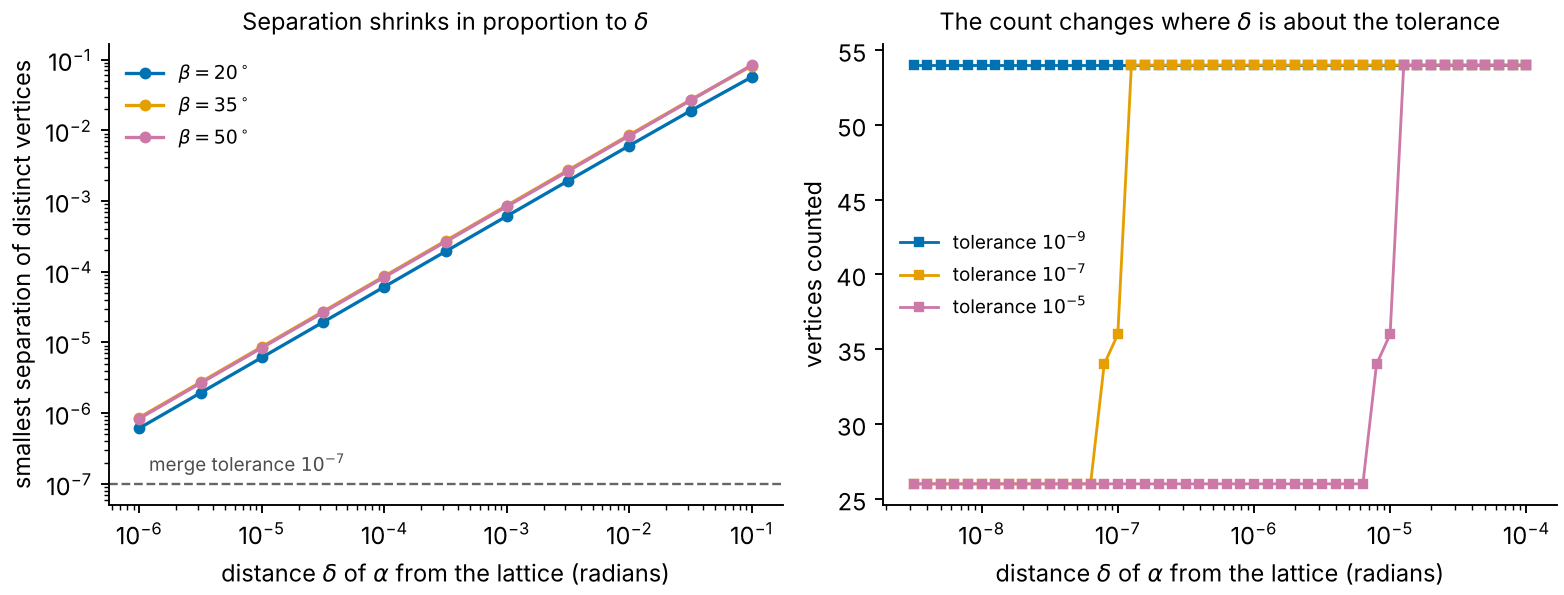
\includegraphics[width=\textwidth]{figs/fig14_boundary.png}
\caption{Left, the smallest separation of two distinct vertices against the distance $\delta$ of $\alpha$ from the lattice, for three values of $\beta$; the dashed line is a merge tolerance of $10^{-7}$. Right, the number of vertices counted at $\beta=35^\circ$ with three merge tolerances. The count drops from $54$ to $26$ where $\delta$ becomes comparable to the tolerance.}
\end{figure}

\section{A Boundary Depends on a Tolerance}

A count made by a program merges points closer than a tolerance, and so the count reports the type of the arrangement only when the tolerance is smaller than the separations that must be resolved and larger than the numerical noise. Near a boundary there is no such tolerance: the separation tends to zero, and any fixed tolerance eventually exceeds it. The right panel of Figure 14.1 shows the consequence. With a tolerance of $10^{-7}$ the count at $\beta=35^\circ$ was $54$ for $\delta\ge1.2\times10^{-7}$, $36$ and $34$ at $\delta=10^{-7}$ and $8\times10^{-8}$, and $26$ below. With a tolerance of $10^{-5}$ the same drop occurs at $\delta\approx10^{-5}$, and with $10^{-9}$ the count stayed at $54$ over the whole range plotted, which ends at $3\times10^{-9}$. The drop completes at about $1.2$ times the tolerance, in agreement with the measured $\delta$-to-separation ratio of $0.86$, and the two intermediate counts show that the vertex pairs merge at slightly different values of $\delta$, since the ratio varies from pair to pair.

The practical consequence concerns what an angle stored in the machine means. A value of $\alpha$ entered as $45^\circ$ in a field that stores single precision is not $\pi/4$ exactly: the stored value is $2.2\times10^{-8}$ radian above it, $90^\circ$ is $4.4\times10^{-8}$ above, and $135^\circ$ is $6\times10^{-9}$ above. For these three the vertex count was $54$ at a merge tolerance of $10^{-9}$ and $26$ at $10^{-7}$ and $10^{-6}$, so whether an arrangement entered on the lattice \emph{is} on the lattice depends on the tolerance of the program that counts it. For $22.5^\circ$ and $5^\circ$ the count was $54$ at all three tolerances. A report that says the arrangement at $\alpha=45^\circ$ has $26$ vertices is a report that the member, as stored, lies within the tolerance of the lattice line, and a careful report states the tolerance. This is the same lesson as the end of Chapter 13, applied to a parameter instead of a normal: the count is a function of the tolerance as well as of the arrangement, and a strata map should list the tolerances for which it is valid.

\section{Members From Specifications}

A generator that produces members of the family must record what it produced and must be safe to run twice. The function in \texttt{param\_sweep.py} builds a member into a collection named from its parameters, for example \texttt{Arrangement a22.5 b30}, stores the specification (parameters, sample count, radius) as a JSON string on the collection, stores the counts computed from the family formula beside it, stores each circle's unit normal on its object, and returns without doing anything if a collection of that name already exists. It was run on five specifications, $(\alpha,\beta)=(0,35)$, $(22.5,30)$, $(10,35)$, $(45,35)$, and $(5,35)$ in degrees, twice in succession.

\begin{center}
\begin{tabular}{lrrrrrr}
\toprule
Collection & $V$ & $E$ & $F$ & Rebuilt $V$ & $E$ & $F$\\
\midrule
\texttt{Arrangement a0 b35} & 26 & 72 & 48 & 26 & 72 & 48\\
\texttt{Arrangement a10 b35} & 54 & 116 & 64 & 54 & 116 & 64\\
\texttt{Arrangement a22.5 b30} & 54 & 116 & 64 & 54 & 116 & 64\\
\texttt{Arrangement a45 b35} & 26 & 72 & 48 & 26 & 72 & 48\\
\texttt{Arrangement a5 b35} & 54 & 116 & 64 & 54 & 116 & 64\\
\bottomrule
\end{tabular}
\end{center}

The first run created five collections, $45$ objects, and $45$ curve datablocks. The second created nothing and left the counts unchanged, which is the idempotence demonstrated for a different script in Chapter 6. The columns on the right were recomputed from the unit normals stored on the objects, without reference to the parameters, and agreed with the counts recorded at construction. The stored normals differed from the family formula's by up to $3\times10^{-8}$, because Blender stores the vectors in single precision, and this is within the window of tolerances found in Chapter 13. The member can therefore be reconstructed from the record in two independent ways, from its specification by the formula and from its stored normals by direct count, and the two agree. What the record does not contain is the tolerance used in counting, and it should, for the reason of the previous section.

\section{What a Sweep Report Should Contain}

A report on a sweep of a parameterised family should state the grid, the list of types found with their counts and the number of grid members of each, the locations of the boundaries between types and a description of how each is approached, and the tolerance under which the counts were made along with the window of tolerances in which they are stable. For this family the report reads: on a one-degree grid there are two types, the lattice type on three lines and the generic type elsewhere; the separation of the vertex pairs that merge is proportional to the distance from the lattice with a constant between $0.6$ and $0.9$; and counts from single-precision data are correct between a tolerance of a few times $10^{-7}$ and about $0.25$, except within a few times the tolerance of the boundary itself, where the count is not an invariant of the geometry.

\begin{exercise}[14.1: A finer grid]
Refine the grid to $0.25^\circ$ in $\beta$ and $2.5^\circ$ in $\alpha$ near $\beta=45^\circ$ and $\beta=60^\circ$, and report whether any third combinatorial type appears. State what a result of ``none'' does and does not establish.
\end{exercise}

\begin{exercise}[14.2: Predict the flip]
For $\beta=50^\circ$ predict, from the measured constant, the value of $\delta$ at which the count at tolerance $10^{-6}$ begins to fall from $54$, and then measure it.
\end{exercise}

\begin{exercise}[14.3: Store the tolerance]
Add the counting tolerance to the stored record of \texttt{param\_sweep.py} and make the reconstruction step report the interval of tolerances over which the rebuilt counts equal the recorded ones.
\end{exercise}

\begin{exercise}[14.4: A third parameter]
Let the polar circles' azimuths be $k\pi/4+\gamma$ for a parameter $\gamma$. Predict which values of $\gamma$ will change the combinatorial type, using the two mechanisms of Chapter 11, and test the prediction on a grid.
\end{exercise}

\part{Distributed Formation}

\chapter{Local Attachment Rules and What a Cluster Establishes}

\section{From a Rule to a Cluster}

Part V studies structures that form without a plan: no part of the structure is placed by a global design, and its shape results from many local events governed by a rule. The first such rule is the simplest one that already produces a surprising object. A single site is occupied. Particles arrive one at a time, wander at random, and stop when they touch the structure. After a few thousand arrivals the structure is a branching cluster with long arms and deep fjords, nothing like the compact blob that a naive picture of random deposition suggests. The process is called diffusion-limited aggregation, and it is used here because it is small enough to state completely and rich enough to show what a simulation can and cannot establish.

A rule is complete only when everything that affects the outcome has been stated. For the version used here the statement is as follows. The sites are the integer points of the plane, and the seed occupies the origin. Each walker starts on a circle of radius $r+5$ about the origin, where $r$ is the distance of the farthest occupied site, at the lattice point nearest a uniformly random angle. It moves one step along a coordinate axis, in one of the four directions with equal probability. If it ever stands at a distance greater than three times its launch radius from the origin it is discarded. If it stands next to an occupied site it joins the cluster with probability $p$, the stickiness, and otherwise continues. Seven things in that paragraph are choices: the lattice, the neighbourhood, the launch radius, the kill radius, the step distribution, the sticking probability, and the random number generator with its seed. Some of them are expected to matter for the result and some are expected not to, and the point of the chapter is to find out which, by measurement.

\section{The Rule as Code}

The rule is short enough to read in full.

\Needspace{26\baselineskip}
\lstinputlisting[language=Python,basicstyle=\ttfamily\footnotesize,breaklines=true,frame=single,columns=fullflexible,keepspaces=true,firstline=9,lastline=32]{dla.py}

This version uses Python's own generator and a set of occupied sites, and it is slow, because a walker from a distance $R$ needs of the order of $R^2$ steps to reach the cluster. The file \texttt{dla.py} also contains a version compiled with the Numba package that follows the identical rule on an array, and the ensembles below use it. The two versions use different random number generators, so they do not produce the same clusters from the same seed, and the check is statistical. With $10$ seeds each at $N=700$, the exponent defined below was $1.737\pm0.118$ for the Python rule and $1.692\pm0.101$ for the compiled one, where the figures after $\pm$ are standard deviations across seeds. The difference, $0.045$, is within one standard error of the difference, $0.049$, so the two versions agree to the precision of the test.

Reproducibility inside one version was checked directly: the same seed gave the same cluster, site for site, and a different seed gave a different one, with only $233$ of $1500$ sites shared between seeds $5$ and $6$, mostly in the early core. The first five sites of seed $5$ were $(0,0)$, $(0,1)$, $(0,2)$, $(0,3)$, $(1,3)$. A cluster is therefore a function of the rule, its parameters, the seed, and the version of the generator, and a record that omits any of these does not reproduce it.

\section{What the Cluster Is}

The standard summary of a cluster is its mass--radius relation. If the first $n$ particles have radius of gyration $R_g(n)$, the root-mean-square distance of the particles from their centroid, a compact cluster of the plane would have $n\propto R_g^2$ and a one-dimensional string would have $n\propto R_g$. A branching cluster has an exponent between, called its fractal dimension $D$:
\[
  n\;\propto\;R_g^{\,D}.
\]
The exponent was estimated by a least-squares line of $\log n$ against $\log R_g$ at $24$ logarithmically spaced values of $n$ from $100$ to $3000$. Over $20$ seeds, each with $3000$ particles, the estimate was $D=1.713$ with a standard deviation across seeds of $0.068$ and a standard error of the mean of $0.015$. Individual clusters gave values from $1.594$ to $1.838$. The radius of gyration at $3000$ particles was $51.8$ with a standard deviation of $1.4$. The value is close to the $1.71$ usually quoted for planar aggregation of this kind in the literature, a comparison recalled from reading and not tested here.

The variation across seeds is the first thing to notice. A single cluster gives $D$ within about $\pm0.07$ of the mean, so a statement of the form ``this cluster has dimension $1.84$'' would be wrong by an amount that is easily mistaken for a property of the model. The standard error of the mean over $20$ seeds, $0.015$, is a statement about the estimator, and it does not include the systematic effects below.

\section{The Fit Window}

The estimated exponent depends on the range of cluster sizes used for the fit. The same $20$ clusters were refitted over different windows.

\begin{center}
\begin{tabular}{rrr}
\toprule
Fit window in $n$ & Mean $D$ & sd across seeds\\
\midrule
20 to 200 & 1.680 & 0.118\\
100 to 600 & 1.691 & 0.105\\
200 to 1000 & 1.726 & 0.108\\
500 to 3000 & 1.728 & 0.069\\
1000 to 3000 & 1.733 & 0.064\\
100 to 3000 & 1.713 & 0.068\\
\bottomrule
\end{tabular}
\end{center}

The estimate drifts upward by about $0.05$ as the window moves to larger clusters, which is more than three standard errors of the full-window value. The drift is a systematic effect: small clusters have not yet developed their branching, and a line fitted through them has a different slope. A report of $D$ should state the window, and the honest summary of this experiment is that $D$ is between $1.68$ and $1.73$ depending on the window, at these sizes. Whether it continues to drift at larger $n$ was not tested.

\section{The Lattice Leaves a Signature}

The rule is stated on a square lattice and the continuum process it stands for has no preferred directions. A measurement can ask whether the lattice shows. For the outer half of each cluster, that is the particles beyond half the largest radius, the amplitude of the $m$-fold angular harmonic $|\langle e^{im\theta}\rangle|$ measures how much the particles favour $m$ directions. For $m=4$ the amplitude, over $20$ clusters of $3000$ particles with about $1440$ outer particles each, was $0.295\pm0.115$ (standard deviation across seeds), against $0.024\pm0.012$ for an isotropic cloud of the same size. The four axis directions are strongly preferred, by a factor of about twelve in amplitude. The two-fold amplitude was $0.235\pm0.138$ and the eight-fold $0.171\pm0.064$, so single clusters are lopsided as well. The axis-aligned arms visible in the left cluster of Figure 15.1 are consistent with this.

This is the limit that most affects what the cluster may be used for. A conclusion about the geometry of branching in general would need the same rule off the lattice, with continuous positions, and the dimension quoted above is a property of the lattice rule. A conclusion about how a branching rule turns local contact into global shape is supported by the experiment, because the lattice is a way of making the rule precise and not a feature that the conclusion depends on.

\section{Stickiness}

The sticking probability $p$ was varied over four values with $12$ seeds each at $N=2000$ and the same fitting procedure, using the window $100$ to $2000$.

\begin{center}
\begin{tabular}{rrrr}
\toprule
$p$ & $D$ (mean $\pm$ sd) & $R_g$ at $N=2000$ & Run time (s)\\
\midrule
1.00 & $1.765\pm0.101$ & 41.2 & 3.9\\
0.50 & $1.727\pm0.088$ & 34.7 & 2.7\\
0.10 & $1.730\pm0.115$ & 22.7 & 1.9\\
0.02 & $2.078\pm0.133$ & 13.6 & 1.4\\
\bottomrule
\end{tabular}
\end{center}

The radius of gyration at fixed $N$ falls steadily with decreasing stickiness, from $41.2$ to $13.6$, so the clusters are visibly more compact. Over the range $p=1$ to $0.1$ the exponent is the same within the scatter, standard errors being near $0.03$, so stickiness changes the size of the cluster for a given number of particles and no change in $D$ was detected. At $p=0.02$ the fitted value, $2.08$, exceeds the dimension of the plane, which no cluster in the plane can have, and so the number is not a dimension at all. The likely reason is that at low stickiness particles penetrate and fill the interior before branching starts, so in this window the cluster is compact at small $n$ and branches at larger $n$, and one straight line through the whole range is the wrong model. That interpretation is an explanation of the number and was not tested by extending the range. The lesson is that a fitted exponent is meaningful only where the data lie on a line, and an exponent outside the physically possible range is a diagnostic that the fit is wrong.

Figure 15.1 shows two clusters from the same seed, $2000$ particles each, with $p=1$ on the left and $p=0.1$ on the right, coloured by arrival order. The radii of gyration are $38.6$ and $21.9$.

\begin{figure}[ht]
\centering
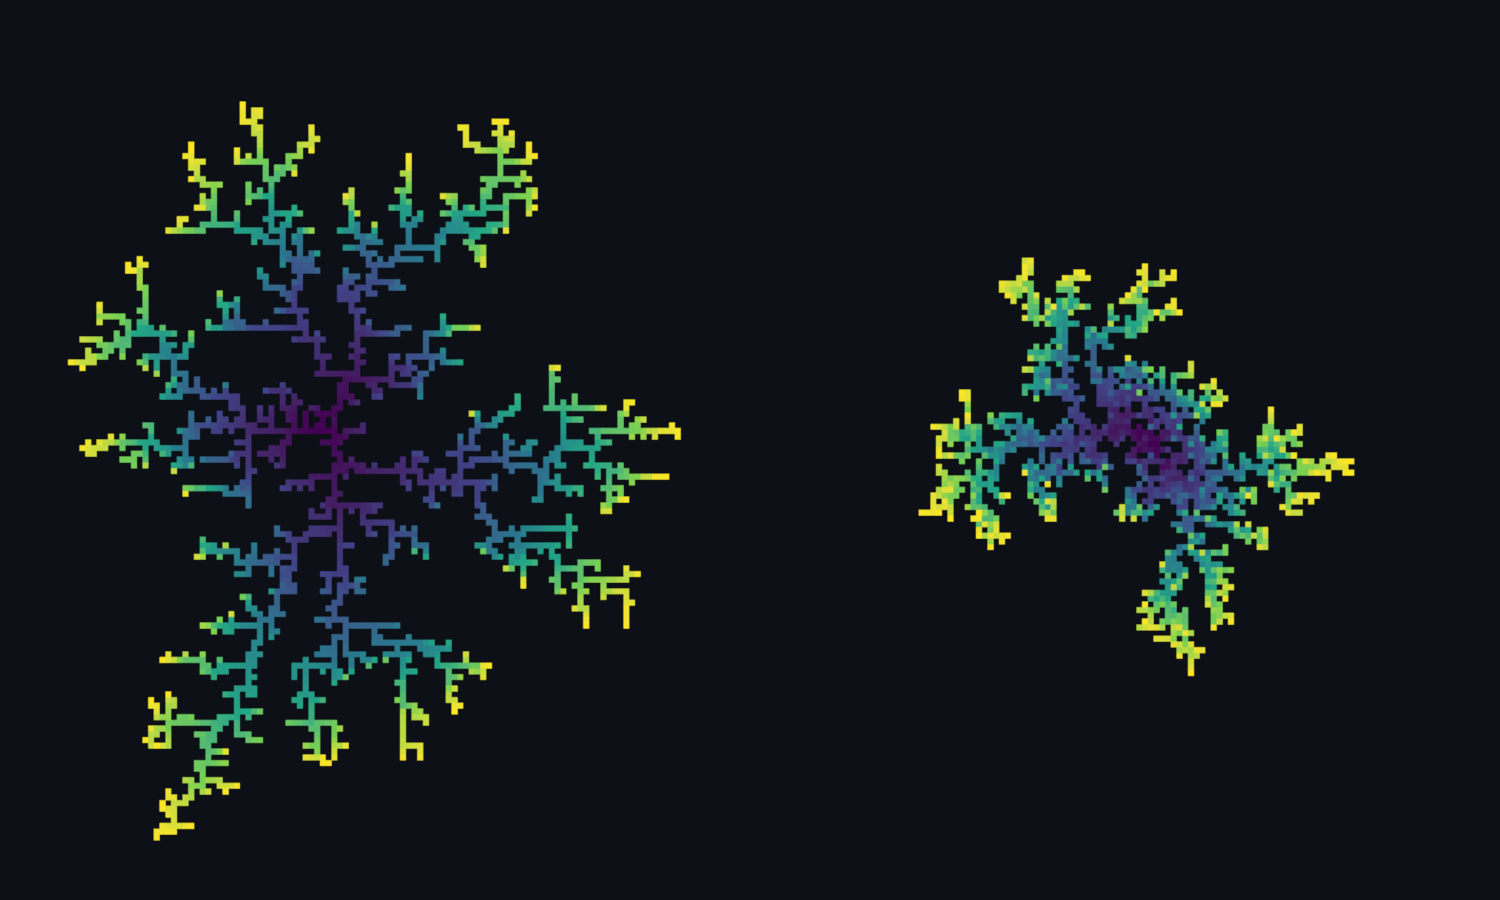
\includegraphics[width=\textwidth]{figs/fig15_clusters.png}
\caption{Two clusters of $2000$ particles with the same seed, $p=1$ (left) and $p=0.1$ (right), viewed from above in Blender with one material that colours each cube by its arrival order, from early (purple) to late (yellow). The radii of gyration are $38.6$ and $21.9$.}
\end{figure}

\section{The Cluster in Blender}

The cluster is brought into Blender as a collection of objects that share one cube mesh, one object per site, in the manner of Chapter 5, with the arrival order stored on each object as a custom property. One material, built as in Chapter 8, reads the property with an Attribute node and maps it through a viridis colour ramp, so the whole cluster uses a single material. The script is \texttt{dla\_blender.py}. For a cluster of $1000$ particles from seed $7$ the scene held $1000$ objects at $1000$ distinct sites, one mesh with $1000$ users, and one material. Every site after the first was adjacent to an earlier one, so the scene is a connected cluster that grew in the recorded order and not a cloud of points; all positions were integers; the stored order matched the creation order; and the seed and stickiness recorded on the collection regenerated the same cluster, site for site. The scene is thus checkable against its own provenance, which is the standard the preceding chapters set for a generated structure.

\section{What the Experiments Do Not Show}

All results are for clusters of at most $3000$ particles on a square lattice, with at most $20$ seeds per condition. The launch offset of $5$ and the kill radius of three launch radii are modelling choices whose effect was not tested, and either could bias the clusters, for instance by discarding walkers that would have reached the tips. The step distribution, the four-neighbour rule, and the generator were not varied. The exponent estimates describe these finite clusters over the windows stated and do not support a claim about the infinite limit. The comparison with the literature value is from recollection. Nothing here shows that a physical process of any particular kind, such as mineral growth, electrodeposition, or the branching of a colony, follows this rule. The experiment shows what the rule does, with a stated precision, and a claim about a physical system would need a separate test of the rule against it.

\begin{exercise}[15.1: Vary the kill radius]
Repeat the dimension estimate at $N=2000$ with kill radii of $2$, $3$, and $5$ launch radii, using $12$ seeds each, and report whether the exponent or the radius of gyration changes by more than the standard error.
\end{exercise}

\begin{exercise}[15.2: Find the crossover]
At $p=0.02$, compute the local slope of $\log n$ against $\log R_g$ in windows of a factor of two in $n$, up to $N=6000$, and describe where the slope crosses from $2$ toward a smaller value.
\end{exercise}

\begin{exercise}[15.3: Off the lattice]
Implement the rule with continuous positions, particles of unit diameter, and sticking on contact, and repeat the harmonic analysis of Section 15.5. State how the four-fold amplitude changes and what that says about the lattice's role.
\end{exercise}

\begin{exercise}[15.4: A record that reproduces]
Write the minimum record from which a cluster in a scene can be regenerated, test it by regenerating from the record alone, and then change one element of the record, such as the version of the generator, and describe what fails.
\end{exercise}

\chapter{Cellular Occupancy and Habitat Spaces}

\section{Occupancy as a Rule}

Chapter 15 grew a structure by adding one particle at a time. A second way of forming structure without a plan keeps the lattice fixed and decides, for every site, whether it is occupied. The simplest such rule treats the sites independently: each site is occupied with probability $p$, by a draw that does not depend on any other site. The result is a random field with a single parameter, and it is the starting point for two questions that matter when the field is meant to be a space that someone can move through. The first is whether the occupied sites, or the empty ones, form a connected region that crosses the whole grid. The second is what a local rule applied repeatedly to the field does to its connectivity. This chapter measures both on a square grid and then places the result in Blender as a habitat floor plan, with the same attention to provenance as before.

Four things have to be stated for the rule to be complete: the grid size $n$, the occupation probability $p$, the notion of adjacency, and the generator with its seed. Adjacency matters because it changes the answer. Two sites are \emph{four-adjacent} if they share an edge and \emph{eight-adjacent} if they share an edge or a corner. A region of occupied sites is a set connected through the chosen adjacency, and a region that touches both the top row and the bottom row is said to span. All counts below use four-adjacency for connection of a region, and the smoothing rule of Section 16.4 uses the eight sites around a cell.

The code is in \texttt{occupancy.py}. The generator is NumPy's \texttt{default\_rng} seeded by an integer, regions are labelled with SciPy's \texttt{ndimage.label}, and a grid built twice from seed $7$ at $n=64$, $p=0.45$ was identical site for site, while seed $8$ differed from it at $2042$ of $4096$ sites. The occupied fraction of the seed-$7$ grid was $0.455$ against a nominal $0.45$, a difference that is ordinary sampling variation, since the standard deviation of the fraction over $4096$ independent sites is $0.008$.

\section{When Occupied Sites Span}

Consider the probability that a random grid of side $n$ has a four-connected occupied region touching both the top and the bottom row. For small $p$ the occupied sites are isolated specks and the probability is near zero, and for $p$ near one it is near one. The interesting question is how sharp the change is and where it sits. The probability was estimated from $400$ seeds at each of seven values of $p$ and four grid sizes.

\begin{center}
\begin{tabular}{rrrrrrrr}
\toprule
$n$ & $p=0.50$ & $0.55$ & $0.58$ & $0.5927$ & $0.61$ & $0.65$ & $0.70$\\
\midrule
32  & 0.013 & 0.125 & 0.335 & 0.440 & 0.635 & 0.915 & 0.990\\
64  & 0.000 & 0.065 & 0.325 & 0.547 & 0.807 & 0.985 & 1.000\\
128 & 0.000 & 0.003 & 0.195 & 0.487 & 0.912 & 1.000 & 1.000\\
256 & 0.000 & 0.000 & 0.072 & 0.515 & 0.983 & 1.000 & 1.000\\
\bottomrule
\end{tabular}
\end{center}

Each entry has a binomial standard error of at most $0.025$. The table shows the change sharpening with $n$: at $p=0.55$ the spanning probability falls from $0.125$ to below $0.005$ as $n$ grows from $32$ to $256$, and at $p=0.61$ it rises from $0.635$ to $0.983$. Curves for different $n$ cross close to $p=0.59$, where the probability is near one half at every size. A sharper measurement of the location is the value of $p$ at which the spanning probability equals one half, found by bisection with $400$ seeds at each step. It was $0.5979$, $0.5907$, $0.5933$ and $0.5925$ for $n=32$, $64$, $128$, $256$. The scatter among the last three, about $0.003$, is of the size expected from $400$ seeds, so the data support a threshold near $0.59$ and no drift in it beyond that scatter. The value usually quoted for site percolation on the square lattice, $0.5927$, is recalled from reading and was not derived here, and these numbers agree with it to the precision measured.

Two points follow for design. A spanning region is not a gradual achievement: a grid with $p=0.55$ of its sites open, which is more than half, is very unlikely to be crossable by four-adjacent steps, and the same grid at $p=0.65$ almost certainly is. And the answer depends on the adjacency, so a rule for walking must be fixed before a field is judged crossable.

\section{Occupancy as a Floor Plan}

A random field is not a plan, but it is the raw material of one common approach to generating caves and ruins, so it is worth stating what the approach would require. Take occupied to mean wall. The open space is the complement, and a visitor can cross it only if the open sites span, so the open-site probability $1-p$ must exceed the threshold, and $p$ must be below about $0.41$. For walls at $p=0.45$ the open fraction is $0.55$, and the table says that open space spanning the grid is rare. A direct count on $200$ grids of $64\times 64$ at $p=0.45$ gave a mean of $200.7$ separate open regions, the largest holding on average $20.2\%$ of the open sites. This is not a space but dust.

\section{A Local Rule Repeated}

The standard remedy is a smoothing rule applied to every cell at once. A cell becomes wall at the next step if at least five of the nine cells in its neighbourhood, itself included, are wall, and becomes open otherwise; cells outside the grid count as wall. The rule is synchronous, so the new grid is computed entirely from the old one. It is the majority rule on an odd number of cells, so it has no ties. Repeated, it either reaches a grid that no longer changes or it does not, and both outcomes occurred.

\begin{center}
\begin{tabular}{rrrrrr}
\toprule
$p$ & Steps & Fixed\,\% & Regions & Largest & Open\\
\midrule
0.40 & $18.4\pm 5.3$ & 100\% & 1.2 & 0.999 & 0.830\\
0.45 & $19.8\pm 7.7$ & 100\% & 2.0 & 0.985 & 0.668\\
0.50 & $22.0\pm13.6$ & 98\%  & 7.3 & 0.665 & 0.444\\
0.55 & $20.9\pm 7.8$ & 100\% & 14.4 & 0.293 & 0.222\\
0.60 & $18.2\pm 5.0$ & 100\% & 11.1 & 0.250 & 0.081\\
\bottomrule
\end{tabular}
\end{center}

The columns give the wall fraction $p$, the steps to a fixed point (mean and standard deviation across seeds), the percentage of grids that reached one within $100$ steps, the number of open regions, the share of open sites in the largest region, and the open fraction after smoothing. The figures are means over $200$ seeds on a $64\times64$ grid, with the region columns taken after smoothing. The rule turns the dust of $p=0.45$ into a nearly single space: $200.7$ open regions before, $2.0$ after, with the largest holding $98.5\%$ of the open sites. The open fraction rises from $0.55$ to $0.668$, which is the rule amplifying the majority, and not a change in the nominal parameter. The same rule at $p=0.55$ goes the other way and closes the field, leaving $14.4$ regions of which the largest holds under a third. The behaviour near $p=0.5$ is a separation between two regimes that the rule creates, a result of the rule and not of the percolation threshold, since smoothing at $p=0.45$ opens a space at an open fraction, $0.55$, below the threshold $0.5927$ that a random field would need.

Five of the $200$ grids at $p=0.5$ did not reach a fixed point in $100$ steps. Examination of those five showed that each had settled into a cycle of period two, four cells flipping on every step. This is a known property of synchronous rules and it is why the statement ``iterate until nothing changes'' is not a safe definition of the procedure: a rule that is run for a fixed number of steps, or that is checked for cycles, always terminates. A grid is declared a fixed point when one step returns it unchanged, so the fixed points reported are fixed by construction.

\section{The Grid in Blender}

Each wall cell becomes an object that shares one cube mesh, in the manner of Chapters 5 and 15, positioned at its integer coordinates and carrying as a custom property the number of wall cells among its eight neighbours. One material reads the property with an Attribute node and maps it from $0$ to $8$ through a two-colour ramp, so edges of walls, which have few wall neighbours, appear in warm colour and wall interiors in dark. The script is \texttt{occupancy\_blender.py}. The random grid and the smoothed grid of seed $3$ at $64\times 64$, $p=0.45$ were built side by side: $1845$ and $1476$ wall objects, one mesh with $3321$ users, and one material. Reading the cell positions back from the scene reproduced both grids exactly, the open regions counted from the scene were $201$ before and $2$ after, with largest-region fractions $0.204$ and $0.994$, regeneration of the smoothed grid from the seed and probability stored on its collection reproduced the scene, the fixed point was reached in $27$ steps, and one further application of the rule left the scene unchanged. Provenance in this chapter has an additional element that Chapter 15 did not need: the rule itself, which is stored as a string on the collection and which would have to match the code that regenerates the grid.

\begin{figure}[ht]
\centering
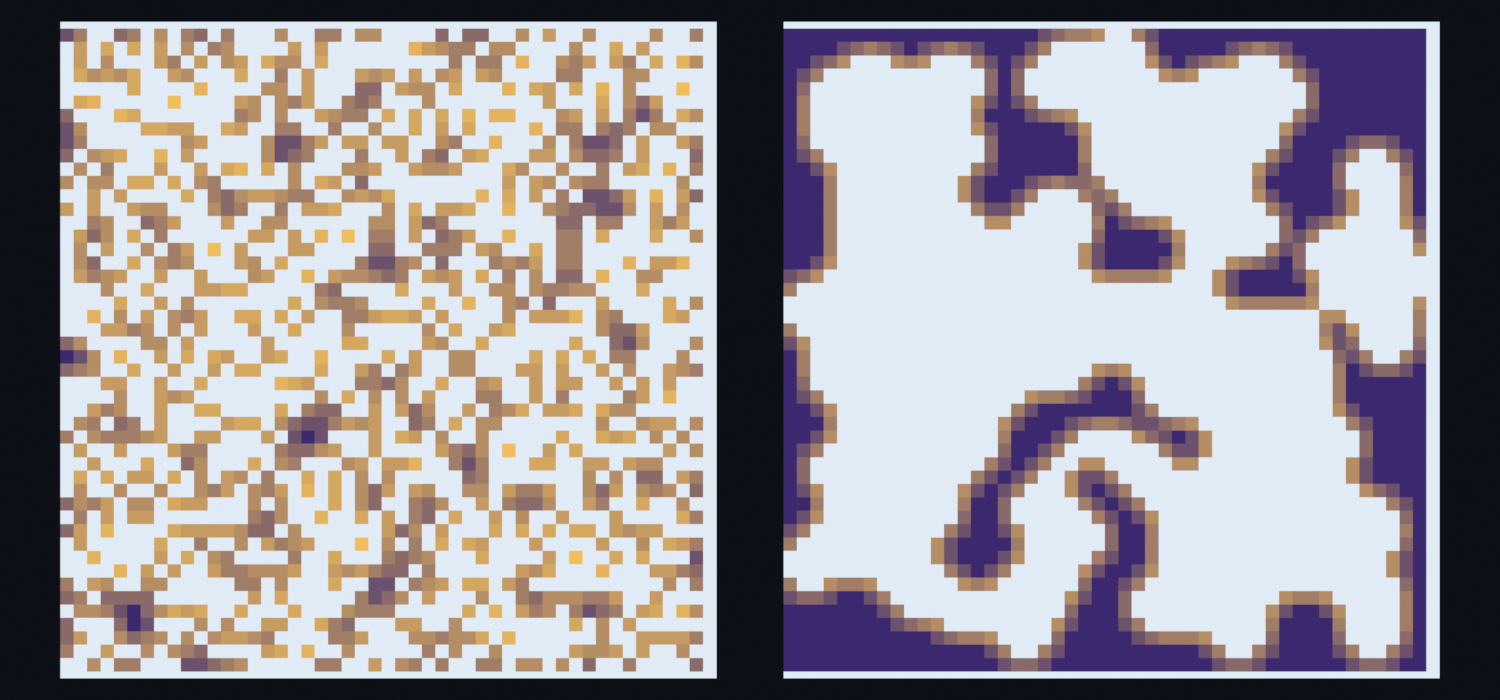
\includegraphics[width=\textwidth]{figs/fig16_caves.png}
\caption{A $48\times48$ random field of walls at $p=0.45$ (left) and the same field after the smoothing rule reached its fixed point (right), seed $3$, viewed from above in Blender. One material colours each wall cube by the number of wall cells among its eight neighbours, warm for few and dark for many. The open region on the right is connected; the field on the left has $133$ open regions and on the right it has $2$.}
\end{figure}

\section{What These Experiments Do Not Show}

All results are for square grids of at most $256\times256$ with four-adjacency for regions, at most $400$ seeds for the spanning estimates and $200$ for the smoothing statistics. The threshold values come from bisection with $400$ seeds per step and are good to about $0.003$; no finite-size scaling analysis was done, so nothing here establishes how the crossing probability depends on $n$ beyond what the table shows. The smoothing rule uses a single threshold of five of nine and a single boundary convention, and neither was varied, so the transition between open and closed outcomes near $p=0.5$ was not located more finely than the five values of the table. The period-two cycles were seen in five grids and were identified by inspection of those grids only. The comparison with the literature threshold is from recollection. Finally, a connected open region is not necessarily a good habitat: nothing was measured about corridor width, dead ends, or sight lines, and Chapter 9 showed that such properties can decide what a visitor can perceive. The experiment shows what the rule does to connectivity, with stated precision.

\begin{exercise}[16.1: Eight-adjacent regions]
Repeat the spanning estimate with eight-adjacency for the occupied region, find the half-probability value of $p$ for $n=128$, and compare it with $1-0.5927$. State why a relationship between the two numbers is to be expected, and test it.
\end{exercise}

\begin{exercise}[16.2: Move the rule]
Change the wall threshold from five of nine to four of nine and to six of nine, and for $p=0.45$ report the open fraction, the number of open regions, and the fraction of grids that cycle. State which of the three rules gives a usable space most often.
\end{exercise}

\begin{exercise}[16.3: Break the cycles]
Replace the synchronous update by one that updates the cells in a fixed scan order. Measure whether period-two cycles still occur, and describe what the change does to the dependence of the result on the seed and on the scan order.
\end{exercise}

\begin{exercise}[16.4: Walk it]
In Blender, place a unit-width walker at an open cell of the smoothed grid and find the shortest four-adjacent route to the farthest open cell. Report its length, compare it with the Manhattan distance between the endpoints, and explain what the ratio says about the corridors.
\end{exercise}

\chapter{Branching and Extinction}

\section{A Process in Which Every Individual Branches}

Chapter 15 grew a cluster by attachment to a structure that already existed, and Chapter 16 filled a lattice site by site. A third way of forming structure lets every existing element produce its own successors, independently of the others. The simplest rule of this kind is the Galton--Watson process. A single individual forms generation zero. Each individual in generation $g$ has a random number of offspring, drawn from one fixed distribution and independently of every other individual, and those offspring make up generation $g+1$. The record of who descended from whom is a rooted tree, and the tree is the object of interest, because a branching structure in a habitat such as a drainage pattern, a root system or a corridor network can be described in the same terms: a rule for how many children each node has, and nothing else.

For the version used here the offspring number is Poisson distributed with mean $m$. Four things must be stated for the process to be reproduced: the offspring distribution and its mean, the rule for stopping a run, the generator, and the seed. The stopping rule matters more than it first appears. A process with $m>1$ may grow without bound, and a process with $m\le 1$ dies out with certainty, but in a finite computation a run can only be stopped, and a run that has been stopped is not a run that has died out. The runs below stop at extinction, at $60$ generations, or when the tree reaches $20{,}000$ individuals, and each run is classified by which of the three happened. A run that reaches the size cap is counted as a survivor in the estimates below, which is an approximation: a tree of $20{,}000$ individuals could in principle still die out, and the probability of that is small and was not measured.

The code is in \texttt{branching.py}. The generator is NumPy's \texttt{default\_rng} seeded by an integer. A run from seed $4$ at $m=1.5$ was identical on repetition, and seed $5$ gave a different tree.

\section{The Extinction Law}

The classical result is that the extinction probability $q$ is the smallest non-negative solution of $q=f(q)$, where $f$ is the generating function of the offspring distribution. For Poisson offspring $f(q)=e^{m(q-1)}$, and the solution is $q=1$ for $m\le1$ and a value below one for $m>1$. The solution was computed by iterating $q\leftarrow e^{m(q-1)}$ from $q=0$, which converges to the smallest root, and then compared it with the fraction of runs that went extinct in an ensemble of $2000$ seeds at each $m$.

\begin{center}
\begin{tabular}{rrrrrr}
\toprule
$m$ & $q$ from the equation & Extinct fraction & Extinct & Size cap & Alive at 60\\
\midrule
0.8 & 1 & $1.0000\pm0.0000$ & 2000 & 0 & 0\\
1.0 & 1 & $0.9605\pm0.0044$ & 1921 & 0 & 79\\
1.2 & 0.6863 & $0.6775\pm0.0105$ & 1355 & 635 & 10\\
1.5 & 0.4172 & $0.4135\pm0.0110$ & 827 & 1173 & 0\\
2.0 & 0.2032 & $0.2090\pm0.0091$ & 418 & 1582 & 0\\
\bottomrule
\end{tabular}
\end{center}

The figures after $\pm$ are binomial standard errors. For $m=1.2$, $1.5$ and $2.0$ the measured fraction differs from the root of the equation by $0.8$, $0.3$ and $0.6$ standard errors, so the ensemble agrees with the equation to the precision of $2000$ runs, with the size-cap approximation included. The row for $m=1.0$ needs a separate reading. The fixed-point iteration for $m=1$ converges so slowly that its output after $2000$ steps, $0.999$, was not used, and the value $1$ in the table is the theoretical one. The measured extinct fraction, $0.9605$, falls below one only because $79$ runs were still alive when stopped at $60$ generations. Those are not survivors in the sense of the theorem. A process at the critical value dies out with certainty, but the time it takes is heavy tailed, and a cut at $60$ generations leaves a few percent still running. For critical processes with finite variance the probability of surviving to generation $n$ is known to fall roughly as $2/(\sigma^2 n)$, which is $0.033$ at $n=60$ for $\sigma^2=1$, against $0.0395$ measured. That formula is recalled from reading and was not derived, and the agreement is of the right size and no more precise than that.

Two lessons for any process run on a computer follow from the table. The classification of a run into extinct, capped and alive must be reported, because the three outcomes are different statements. And a result at the critical value of a parameter depends on the stopping rule, so a figure such as $0.9605$ is a property of the run length as much as of the process.

\section{Total Size at the Critical Value}

At $m=1$ every run is finite, so it has a total number of individuals $T$, and the distribution of $T$ has a heavy tail. For $4000$ seeds, with runs allowed up to $400$ generations and $100{,}000$ individuals, the fraction with $T\ge t$ was $0.6375$, $0.2677$, $0.0875$ and $0.0312$ for $t=2$, $10$, $100$ and $1000$. The product of this fraction with $\sqrt t$ was $0.902$, $0.847$, $0.875$ and $0.988$. A tail of the form $P(T\ge t)\propto t^{-1/2}$ would make the product constant, and the measured values are close to constant, within the sampling error of the last, which is about $0.09$ from $4000$ runs. A tail exponent of one half over three decades in $t$ is therefore consistent with the data. The longest critical tree among the first $300$ seeds that went extinct had $11{,}590$ individuals and the typical one far fewer, so the mean size is not a useful summary of a critical process. The exponent is a statement about this ensemble, and the constant in the tail, which was not compared with a theoretical value, is not claimed.

\section{One Realisation in Blender}

A realisation is a tree, and a tree is placed in Blender as one object per edge, all sharing one box mesh scaled to the length of the edge and rotated to its direction, in the manner of Chapters 5, 15 and 16. Each edge carries its generation as a custom property, one material reads it with an Attribute node, and the layout is the standard tidy one in which leaves have consecutive horizontal positions in depth-first order and each parent sits at the mean position of its children. The script is \texttt{branching\_blender.py}.

A critical realisation was chosen as the first seed whose run went extinct with between $150$ and $300$ individuals. The first such seed was $1$, with $166$ individuals, and the scene held $165$ edge objects, one mesh with $165$ users and one material. The edge objects formed a tree in the exact sense that there were $n-1$ edges, every node except the root appeared as a child exactly once, and every parent was created before its child, so there were no cycles. The generation stored on each edge equalled the generation recomputed from the edge list, the position of each edge matched the midpoint of its endpoints in the layout to $4\times10^{-6}$, and the tree regenerated from the stored seed and mean reproduced the scene individual for individual. The population by generation of this tree was $1,2,2,1,2,2,1,1,3,3,4,4,5,6,11,13,8,10,15,13,15,11,6,5,6,6,8,2$, so it reached generation $27$ and then ended, having never exceeded fifteen individuals in a generation. This is typical of the critical process, which survives for a long time at small width and then dies.

\begin{figure}[ht]
\centering
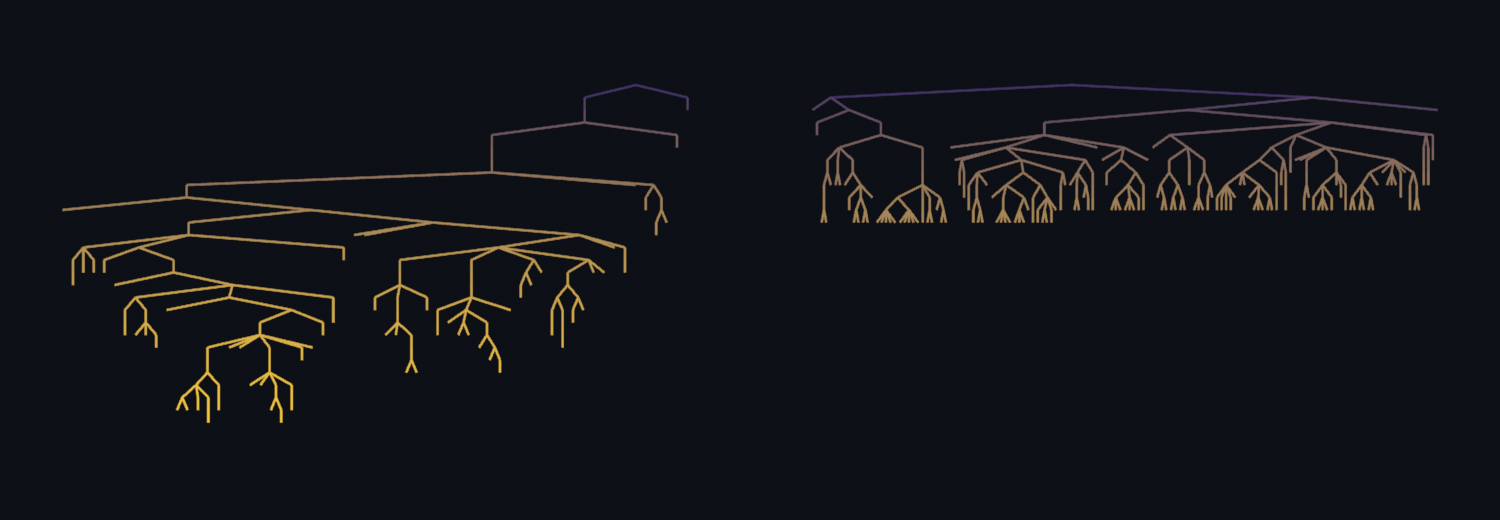
\includegraphics[width=\textwidth]{figs/fig17_trees.png}
\caption{Left, a critical realisation ($m=1$, seed $1$) that went extinct at generation $27$ with $166$ individuals. Right, a supercritical realisation ($m=1.5$, seed $1$) stopped at $300$ individuals, which reached generation $11$. Edges are coloured by generation from early (purple) to late (yellow), with one material and a colour scale running to generation $28$ in both trees. Each tree is drawn to the same width, so the horizontal scales differ.}
\end{figure}

The supercritical tree on the right was stopped at the size cap during a generation, so its last generation is incomplete, and the truncation falls on the later individuals by construction. It is shown to give the visual contrast of a wide and shallow tree against a narrow and deep one, and it is not a sample from which any statistic in this chapter was computed.

\section{What These Experiments Do Not Show}

All results are for Poisson offspring with five values of the mean, $2000$ runs at each in the extinction table and $4000$ at the critical value, with stopping rules stated above. Nothing was varied in the offspring distribution, so the agreement with the extinction equation does not show that the equation is the right description of a process with a different distribution, and the critical tail was not compared across distributions. The count of capped runs as survivors is an approximation whose error was not bounded. The $60$-generation cut produced the entire gap between the measured and the theoretical extinct fraction at $m=1$, and that attribution rests on the count of $79$ runs alive at the cut and was not tested by lengthening the run. The tail exponent was estimated by constancy of a product over four values of $t$ and not by a fit. The theoretical formulas for the critical process are recalled from reading. Finally, nothing here shows that any physical branching structure follows a branching process: independence of offspring, the absence of competition for space, and the lack of any geometry in the layout are assumptions of the rule, and the layout in the figure is a drawing of a tree, not a model of how the tree would occupy space.

\begin{exercise}[17.1: Another offspring law]
Replace the Poisson distribution by a distribution that takes the values $0$ and $2$ with equal probability, which has mean $1$ and a different variance. Measure the fraction alive at generation $60$ and compare it with the Poisson value. State what quantity the difference should be proportional to, and test the claim.
\end{exercise}

\begin{exercise}[17.2: Bound the size cap]
For $m=1.2$, rerun the extinction ensemble with caps of $2000$, $20{,}000$ and $200{,}000$ individuals, and report whether the extinct fraction changes by more than its standard error. State what that says about the survivor approximation.
\end{exercise}

\begin{exercise}[17.3: A branching rule with space]
Give each child a position displaced from its parent by a unit step in a random direction, and count the pairs of nodes closer than $0.3$ in trees of about $300$ individuals at $m=1.5$. State what the count says about whether the independence assumption could describe a structure that occupies the plane.
\end{exercise}

\begin{exercise}[17.4: Rebuild from the edge list]
Given only the edge objects in a saved scene, recover the number of individuals in each generation and test your recovery against the list printed in Section 17.4. Then delete one edge object and describe which checks of that section detect the loss.
\end{exercise}

\chapter{Foam-Like Cells and Relaxation}

\section{Space Divided Among Seeds}

A third kind of cellular structure divides space instead of filling it. Given a set of points, assign every location to the nearest point. The set of locations assigned to one point is its cell, the cells are convex polygons in the plane, and together they tile it. The tiling is the Voronoi diagram of the points. It describes, to a first approximation, the cells of a dry foam, the territories of animals that defend the ground nearest their nests, the catchments of wells, and the plan of a market in which each customer visits the nearest stall. In each case the points are the primary data and the cells are a derived structure, so the useful questions concern what the cells inherit from the points. This chapter asks what a random arrangement of points produces, how an iterative rule that moves each point towards the centre of its own cell changes the arrangement, and what can be measured to say so.

To avoid edge effects, all arrangements are placed on a torus, the unit square with opposite sides identified, and computed by tiling nine copies of the points and keeping the cells of the central copy. The cells of the central copy are polygons that may extend past the square, and together they cover it exactly once. The code is in \texttt{foam.py}. It uses SciPy's \texttt{Voronoi}, orders each cell's vertices by angle about its point, and counts a side wherever consecutive vertices are distinct. The generator is NumPy's \texttt{default\_rng}, and the same seed gave the same points and the same side counts on repetition.

\section{Two Identities That Hold for Every Arrangement}

Two properties were checked on five random arrangements of $400$ points before any statistics were taken. The cell areas summed to $1$, to the twelve decimals printed, so that the cells tile the torus with neither gap nor overlap. The mean number of sides was $6$ exactly, in every arrangement. The second property is an instance of Euler's formula. On a torus a polygonal tiling has $V-E+F=0$, and when three cells meet at every vertex, as happens with probability one for random points, each vertex has three edges, so $2E=3V$ and the average cell has $2E/F=6$ sides. The identity says nothing about the points, and it holds for the regular hexagonal tiling and for the most irregular one alike. It follows that the mean number of sides cannot distinguish arrangements, and the quantities that can are the spread of the side counts and the spread of the cell areas.

\section{Random Points and Relaxed Points}

The relaxation rule, usually attributed to Lloyd, moves every point to the centroid of its cell and recomputes the cells. One application is one step. The rule does not change the number of points, and it is deterministic once the starting points are fixed, so an arrangement is a function of the seed and the number of steps. The statistics below are means over $20$ seeds of $400$ points each, with the standard deviation across seeds after each $\pm$. The side-count spread is the standard deviation of the number of sides within one arrangement, the hexagon fraction is the share of cells with exactly six sides, and the area spread is the standard deviation of cell area divided by its mean.

\begin{center}
\begin{tabular}{rrrrr}
\toprule
Steps & Mean sides & Side-count spread & Hexagon fraction & Area spread\\
\midrule
0  & $6.000\pm0.000$ & $1.346\pm0.040$ & $0.287\pm0.021$ & $0.522\pm0.033$\\
1  & $6.000\pm0.000$ & $1.069\pm0.041$ & $0.376\pm0.024$ & $0.373\pm0.028$\\
2  & $6.000\pm0.000$ & $0.945\pm0.025$ & $0.418\pm0.025$ & $0.303\pm0.026$\\
5  & $6.000\pm0.000$ & $0.811\pm0.021$ & $0.481\pm0.032$ & $0.212\pm0.024$\\
10 & $6.000\pm0.000$ & $0.718\pm0.028$ & $0.550\pm0.027$ & $0.157\pm0.021$\\
20 & $6.000\pm0.000$ & $0.628\pm0.025$ & $0.623\pm0.026$ & $0.114\pm0.018$\\
50 & $6.000\pm0.000$ & $0.544\pm0.019$ & $0.705\pm0.022$ & $0.074\pm0.009$\\
\bottomrule
\end{tabular}
\end{center}

The first step does the most work: the area spread falls from $0.522$ to $0.373$. After that the improvement slows. The area spread falls by about a third between steps $20$ and $50$, and the side-count spread falls by about a seventh. Even after $50$ steps, $29.5\%$ of the cells are not hexagons, so the arrangement has not become a regular lattice, and the departures from six sides persist. In the relaxed Blender example of Section 18.5 the non-hexagons are almost all five-sided or seven-sided, $36$ and $32$ of $150$ cells. Whether the hexagon fraction would approach one with many more steps was not tested, and the table gives no reason to assume that it does.

For the random arrangement the spread of the side counts, $1.346$, corresponds to a variance of $1.81$, and the area spread, $0.522$, can be compared with the values recalled, and not rechecked, from the literature on random Voronoi tessellations of about $1.78$ and $0.53$. The agreement is within the seed-to-seed scatter, and the literature values are recalled and were not checked against a source.

\section{Large Cells Have More Sides}

In dry foams larger cells tend to have more sides, a relation named for Lewis that is usually stated as a linear dependence of mean area on the number of sides. The relation was measured on the random arrangements, pooling $8000$ cells from the $20$ seeds, with each cell's area divided by its arrangement's mean area.

\begin{center}
\begin{tabular}{rrrrrrrrr}
\toprule
Sides & 3 & 4 & 5 & 6 & 7 & 8 & 9 & 10\\
\midrule
Cells & 84 & 905 & 2052 & 2299 & 1631 & 691 & 266 & 60\\
Mean relative area & 0.384 & 0.561 & 0.780 & 0.997 & 1.210 & 1.450 & 1.700 & 1.856\\
\bottomrule
\end{tabular}
\end{center}

A straight line fitted to the means for $4$ to $8$ sides has slope $0.219$ per side and reaches zero area at $1.45$ sides, so the dependence is close to linear over that range, with the six-sided cell very close to average. The slope at the ends departs a little: from $3$ to $4$ sides the area rises by $0.177$, and from $9$ to $10$ by $0.156$, against $0.219$ in the middle. The measurement shows a monotone, nearly linear increase for these arrangements. It does not test the relation as a law of foams, because a random point set is not a foam, and it does not settle why the relation holds. After relaxation the cells have nearly equal areas, so the relation weakens as the arrangement approaches a regular one, and that was not measured.

\section{Cells in Blender}

All cells of an arrangement are placed in Blender as one mesh with one polygon per cell. The number of sides is stored as an integer attribute on each face, and one material reads that attribute with an Attribute node of the geometry type and maps it from $4$ to $8$ through a blue--white--red ramp, so the whole arrangement uses one object, one mesh and one material. This differs from the preceding chapters, where the quantity of interest was stored on each object, and the choice here follows from the structure: the cells belong together as one tiling, and sharing one mesh preserves their adjacency. The script is \texttt{foam\_blender.py}.

For $150$ points from seed $2$, before and after $20$ relaxation steps, the mesh held $150$ polygons in each case, and the polygon areas summed to $1.000000$, which is the area of the torus, so the mesh tiles the square exactly as the calculation did. The mean number of sides read from the stored attribute was $6.0000$ in both cases. The attribute equalled the number of vertices of each polygon for every cell. The histogram of side counts for $3$ through $10$ sides was $1,15,43,45,24,16,4,2$ for the random points and $0,0,36,80,32,2,0,0$ after relaxation, so the relaxed arrangement has no cell with fewer than five or more than eight sides. The relaxed points were regenerated from the seed and the step count and were identical. Under $20$ steps the points moved on average by $0.044$ of the side of the square, which is about half of the mean spacing of about $0.082$ for $150$ points.

\begin{figure}[ht]
\centering
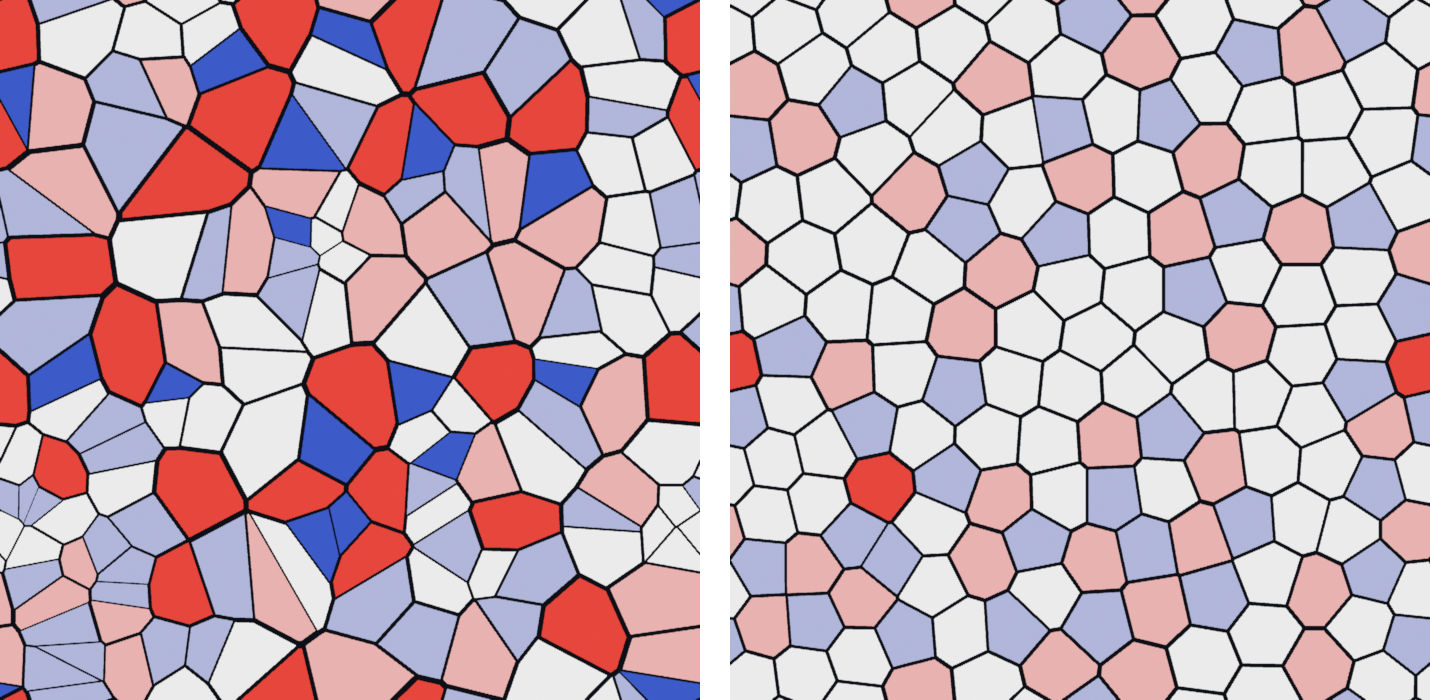
\includegraphics[width=\textwidth]{figs/fig18_foam.png}
\caption{The unit torus tiled by $150$ cells coloured by number of sides, from four (blue) through six (white) to eight (red), with one material reading a face attribute. Left, random points, seed $2$. Right, the same points after $20$ relaxation steps. The panels were rendered separately from the same mesh construction, with the cells drawn at $0.94$ of their size so that the walls are visible. Thin cells at left are real cells of the random arrangement, and the area sum confirms that the tiling is complete.}
\end{figure}

\section{What These Experiments Do Not Show}

All results are for points on a torus, with $400$ points in the tables and $150$ in the Blender scene, and with $20$ seeds for the statistics, so edge effects, which dominate small real foams, were excluded by construction. The relaxation rule was stopped at $50$ steps, and nothing was measured about its limit. The side-count and area spreads for random points are compared with literature values that are recalled from reading. The linear relation of area to number of sides was observed over a pooled sample and not tested for other densities or for relaxed arrangements. Nothing here shows that a real foam, a territory pattern or a market follows the Voronoi rule, which assigns each location to the nearest point and ignores the surface tension, the competition and the travel costs that govern the real systems. The experiments show what a nearest-point rule does with random and relaxed points, with the precision stated.

\begin{exercise}[18.1: Many more steps]
Run the relaxation for $200$ and $1000$ steps on $10$ seeds of $400$ points, report the hexagon fraction at each, and say whether the table's trend continues. State what a stable fraction below one would mean for the structure.
\end{exercise}

\begin{exercise}[18.2: Density]
Repeat the random-points statistics at $100$, $400$ and $1600$ points, and report whether the side-count spread and area spread depend on the number of points. State what you expect before running it.
\end{exercise}

\begin{exercise}[18.3: A different seed process]
Replace the uniform random points by points placed with a minimum separation (a hard-core process) and compare the side-count spread and area spread with the random case and with the relaxed case at the same number of cells. Describe where the hard-core arrangement falls between them.
\end{exercise}

\begin{exercise}[18.4: Walls as edges]
Extract the shared edges of one relaxed arrangement from the mesh, count them, and check the relation $2E=3V$ implied in Section 18.2. Report any vertex at which four cells meet and the tolerance you used to decide.
\end{exercise}

\chapter{Resource Transport on Adaptive Networks}

\section{A Network That Responds to Its Own Load}

The preceding chapters of Part V formed structures from rules of attachment, occupancy, branching and division. A structure that carries something, such as water through channels, nutrients through a fungal mat, or traffic through streets, raises a further question: what happens when the carrying capacity of each link responds to how much it carries? Slime moulds, vein networks and river basins are often described in these terms, and a short rule of this kind is simple enough to state completely, run, and check in Blender. This chapter uses the rule to close Part V and to introduce the coupling between a numerical solver and a scene that Part VII develops.

The network is a square grid of $16\times16$ nodes with $480$ unit-length edges. Each edge $e$ has a conductance $D_e$. One corner node injects a unit of flow and the opposite corner removes it. Given the conductances, the flow is fixed by conservation at every node together with Ohm's rule that the flow in an edge equals its conductance times the pressure difference between its ends. That is a linear system, solved here by direct elimination with the sink grounded at zero pressure. The conductances then adapt: each is moved towards a function of the flow it carries,
\[
  \frac{dD_e}{dt}=f(|Q_e|)-D_e,\qquad f(q)=\frac{q^\mu}{1+q^\mu},
\]
integrated by explicit steps of $0.3$. The exponent $\mu$ is the one free parameter and controls how strongly a loaded edge is reinforced. For $\mu=1$ the reinforcement is linear in the flow for small flows, for $\mu>1$ it is disproportionately strong for busy edges, and for $\mu<1$ weak edges are reinforced relatively more. A rule of this form is used in models of the slime mould \emph{Physarum}, as recalled from reading and not rechecked, and the precise form above is an assumption of this chapter and not a reproduction of a particular paper. Initial conductances are $1$ plus noise of standard deviation $0.05$, clipped below at $0.5$, drawn from a seeded generator. The code is in \texttt{transport.py}.

\section{What the Solver Must Satisfy}

A solver is trusted only after it has been checked against what it must satisfy whatever the conductances. With all conductances equal to one, the node balance, the net flow out of each node less the prescribed injection, had a largest absolute value of $5.8\times10^{-15}$ over the $256$ nodes, the two edges at the source carried $0.5$ each, and no edge carried more than $0.5$. These checks verify conservation and symmetry. They do not verify that the model describes any physical network, which is a separate question. The same balance residual was computed after every adaptation run below and was at most $4\times10^{-15}$ in the runs inspected individually, so the flows reported are exact solutions of the stated equations to floating-point precision at the final state.

\section{The Effect of the Exponent}

For seven values of $\mu$, ten seeds each, the adaptation was run for $1500$ steps and the final network was summarised by four numbers. An edge is counted as kept if its conductance exceeds $0.01$. The cycles are the independent loops of the kept network, computed as kept edges minus kept nodes plus one. The total conductance is the sum over all edges. The dissipation is $\sum_e Q_e^2/D_e$, the power that the flow dissipates in the network, in units where the unit flow and unit edge length are fixed.

\begin{center}
\begin{tabular}{rrrrr}
\toprule
$\mu$ & Edges kept & Cycles & Total conductance & Dissipation\\
\midrule
0.5 & $480.0\pm0.0$ & $225.0\pm0.0$ & $88.68\pm0.00$ & $13.10\pm0.00$\\
0.8 & $480.0\pm0.0$ & $225.0\pm0.0$ & $43.57\pm0.00$ & $22.15\pm0.00$\\
1.0 & $452.0\pm0.0$ & $199.0\pm0.0$ & $27.04\pm0.00$ & $33.61\pm0.00$\\
1.2 & $73.6\pm7.2$ & $9.1\pm1.7$ & $18.50\pm0.19$ & $48.66\pm0.48$\\
1.5 & $30.0\pm0.0$ & $0.0\pm0.0$ & $15.00\pm0.00$ & $60.00\pm0.00$\\
2.0 & $30.0\pm0.0$ & $0.0\pm0.0$ & $15.00\pm0.00$ & $60.00\pm0.00$\\
3.0 & $30.0\pm0.0$ & $0.0\pm0.0$ & $15.00\pm0.00$ & $60.00\pm0.00$\\
\bottomrule
\end{tabular}
\end{center}

The figures after $\pm$ are standard deviations over the ten seeds. The change is sharp. At $\mu\le1$ the whole grid, or nearly all of it, carries flow, with $199$ to $225$ independent loops, and at $\mu\ge1.5$ the final network is a single path of $30$ edges with no loop at all. The value $30$ is the length of the shortest route between opposite corners of the grid, $15+15$ steps, and the total conductance of that path, $15$, is $30$ edges at $0.5$ each, which is $f(1)$ for a unit flow. Its dissipation, $60$, is $30\cdot1^2/0.5$. The intermediate value $\mu=1.2$ gives a sparse network with about seventy-four edges and nine loops, and is the only row where the outcome varies between seeds.

Three quantities move in opposite directions. As $\mu$ rises the total conductance, which stands for the material invested in the network, falls from $88.7$ to $15.0$, and the dissipation, which stands for the cost of using it, rises from $13.1$ to $60.0$. The rule has no budget in it, so neither quantity is optimised, and the comparison is a description of what the rule produces. For $\mu=1$ the final network has $452$ edges and is the same for all ten seeds, with no variation at the precision shown. For the larger exponents the path is a shortest path, and which of the very many shortest paths on the grid is chosen does depend on the seed: for $\mu=1.5$ the kept edge sets of four seeds were four different paths. It is consistent with these results that at $\mu=1$ the network settles on the whole family of shortest routes, since every edge of the grid lies on some monotone route between opposite corners, but that was not tested explanation.

\section{When the Run Has Finished}

The reported networks are steady states only if the iteration has converged. The largest rate of change of any conductance after the last step, in units of change per unit of time, was below $10^{-14}$ for $\mu=0.5$, $0.8$, $1.5$, $2.0$ and $3.0$, $8.5\times10^{-8}$ for $\mu=1.0$, and up to $4.4\times10^{-4}$ in the slowest of the ten seeds at $\mu=1.2$. The last of these is small but not zero, and the row for $\mu=1.2$ should be read as nearly converged. For one seed at $\mu=1.2$ a run of $400$ steps gave $76$ edges and $12$ cycles and one of $1500$ steps gave $74$ edges and $11$ cycles, so the counts were still changing slowly at $400$ steps, and the reported numbers depend on the run length by a few edges. A finite run is a stopping rule, and the table's counts at the critical region are properties of the rule and the run length, as in Chapter 17.

\section{The Network in Blender}

The network is placed in Blender with one object per edge, all sharing one box mesh, in the manner of Chapter 17. The width of each edge is set from its conductance, $0.06+0.9D_e$, and the magnitude of the flow is stored on the object as a custom property that one material reads and maps from $0$ to $0.5$ through a two-colour ramp, so width and colour carry two different quantities of the same state. The script is \texttt{transport\_blender.py}. The scene for $\mu=1.2$ and seed $0$ held $480$ edge objects, one mesh with $480$ users and one material. The edge list read back from the scene equalled the generated list, and the conductances recovered from the widths matched the originals to $1.6\times10^{-8}$. A solver run on the recovered conductances reproduced the stored flows to $2.3\times10^{-8}$ and satisfied node balance to $1.8\times10^{-14}$. There were $74$ edges with conductance above $0.01$, and the total conductance was $18.475$ in the scene and in the generation. The network regenerated from the stored seed, exponent and step count was identical to the scene within $10^{-5}$.

This is the first scene in the book in which Blender and a solver exchange state in both directions. The solver produced the state, Blender held it as geometry and properties, and a solver run from the geometry alone recovered the same flows, which shows that the representation preserved what the solver needs. The figure shows four networks from the same seed at $\mu=0.5$, $1.0$, $1.2$ and $1.5$.

\begin{figure}[ht]
\centering
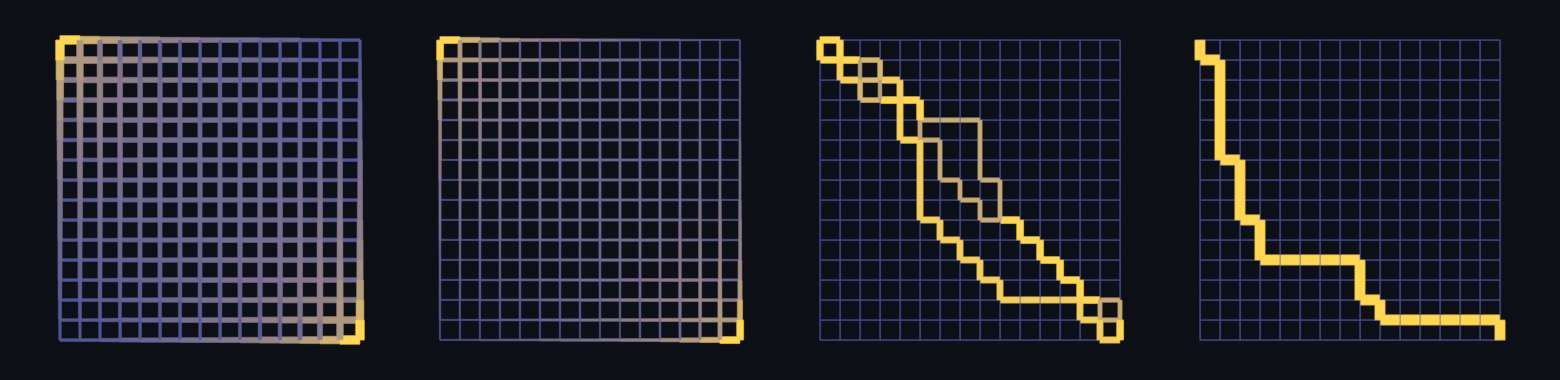
\includegraphics[width=\textwidth]{figs/fig19_networks.png}
\caption{Adapted networks on a $16\times16$ grid with the source at the upper left and the sink at the lower right, for $\mu=0.5$, $1.0$, $1.2$ and $1.5$ from left to right, seed $0$. Edge width is $0.06+0.9D$ and colour shows the flow from $0$ (blue) to $0.5$ (yellow), by one material reading a custom property.}
\end{figure}

\section{What These Experiments Do Not Show}

All results are for one grid size, $16\times16$, one source and sink position, one noise level, and one integration step, with ten seeds per exponent and $1500$ steps. The exponent values are a coarse sample, and the location of the transition between $\mu=1.0$ and $\mu=1.5$ was not found more finely than the row for $1.2$. The $\mu=1.2$ row is nearly but not exactly converged. Nothing was varied in the form of the reinforcement function, in the grid, or in the conductance floor of $0.01$ that decides which edges count as kept, and the cycle count depends on that floor. The statement that the rule is used for the slime mould is recalled from reading. Nothing here shows that any biological or engineered network follows the rule, nor that its parameters correspond to measured quantities, and the total conductance and the dissipation are quantities of the model and not of a material. The Blender scene shows that the solver's state survives translation into geometry and back. It is not a check of the model.

\begin{exercise}[19.1: Locate the transition]
Run $\mu=1.05$, $1.1$, $1.15$, $1.25$, $1.3$ and $1.4$ on ten seeds, with enough steps that the largest rate of change falls below $10^{-8}$, and report the number of kept edges for each. State the smallest exponent at which every seed gave a single path.
\end{exercise}

\begin{exercise}[19.2: Another source]
Move the sink from the opposite corner to the middle of the far edge and repeat the runs at $\mu=0.8$, $1.0$ and $1.5$. State how the length of the final path and the number of loops depend on the geometry, and compare the lengths with the shortest route.
\end{exercise}

\begin{exercise}[19.3: A budget]
After each adaptation step, rescale the conductances so that their sum stays at $30$. Repeat the exponent sweep and report whether the dissipation is now minimised near any exponent. State what the constraint changes about the comparison in Section 19.3.
\end{exercise}

\begin{exercise}[19.4: Read it from the scene]
Delete one edge object from the saved scene of Section 19.5 and re-solve from the remaining geometry. Report which of the checks of that section detect the change, and what the balance residual shows.
\end{exercise}

\part{Python and Reproducible Construction}

\chapter{Inspecting a Scene and the Two Ways to Act on It}

\section{Why Python Changes the Kind of Work}

Part V ran every experiment from a script, and the scripts shared habits that were never stated: they built objects from data, they put generated objects in collections of their own, they checked what the scene held, and they could rebuild it from a seed. Part VI states those habits as a method. Blender's Python interface offers two ways to act on a scene that look alike in a short example and behave very differently in a long program. One imitates the interface: an operator such as \texttt{bpy.ops.mesh.primitive\_cube\_add} does what the menu item does, using the current selection, the active object and the active collection. The other edits the data directly: \texttt{bpy.data.objects.new} creates an object and nothing else. This chapter measures the difference, shows what each leaves behind in the scene, and builds two small tools, an inventory of what a scene contains and a way of clearing generated content without touching anything else. All measurements were made in the headless Blender 5.2.2 used throughout, with a factory-reset empty scene at the start of each probe. The scripts are \texttt{scene\_tools.py} and \texttt{ch20\_probe.py}.

\section{Three Parts of the Interface}

The module \texttt{bpy} has three parts that matter here. The first, \texttt{bpy.data}, holds every data-block in the file as named collections: objects, meshes, materials, collections, cameras and so on. It is a database, and it is available whatever the interface is doing. The second, \texttt{bpy.context}, describes the present state of the interface: the active object, the selected objects, the current scene and mode. Its contents change as operators run. The third, \texttt{bpy.ops}, is the set of operators, each a command that reads the context, makes changes and may fail if the context does not suit it. A script that mixes these without noticing which it is using will behave differently when run from a different starting state.

\section{What Each Leaves Behind}

A cube was created by operator in an empty scene and a triangle was created by the data interface, and the scene was examined before, between and after. Before anything, there was no active object, no selection, and no objects or meshes. After \texttt{primitive\_cube\_add}, the new object was active and selected, its mesh was named Cube, and it belonged to the scene's master collection and not to the collection named Generated that the script had made. After the triangle was created with \texttt{bpy.data.meshes.new}, \texttt{from\_pydata} and \texttt{bpy.data.objects.new}, the active object was still the cube, the selection still held one object, and the triangle was in Generated because the script linked it there. The operator therefore changes the interface state and places the result by context, while the data interface changes what it is told to change.

Operators also depend on a context that may be absent. In an empty scene, \texttt{bpy.ops.object.mode\_set(mode='EDIT')} raised a \texttt{RuntimeError} with the message ``Operator bpy.ops.object.mode\_set.poll() Context missing active object'', and after a cube had been added it ran and put the object in edit mode. The failure is a poll failure: each operator first asks whether the context permits it. A script that depends on an active object must establish one, and a script that never uses an operator never meets the question.

\section{What Names Are and Are Not}

A name is a label for a data-block within its collection and it is not a stable identity. Three objects created with the name Wall were named Wall, Wall.001 and Wall.002. When the first was removed and a new object was requested with the name Wall, the new object received the name Wall, the freed name, and the existing objects were Wall, Wall.001 and Wall.002 as before. A record that says ``the object called Wall'' therefore refers to a different object after the sequence than before. A script that must find its own objects later should record something that survives, such as the generated collection they were placed in, a custom property holding an identifier of its own, or the parameters from which they can be rebuilt, which is the approach of Chapters 15 to 19.

\section{Orphans}

Removing an object does not remove its mesh. After a mesh with one user was linked into an object and the object was removed through \texttt{bpy.data.objects.remove}, the mesh was still in \texttt{bpy.data} with zero users. The call \texttt{bpy.data.orphans\_purge(do\_recursive=True)} then removed it, and returned $1$. Whether a zero-user block survives a save is a separate question, and it was tested: a mesh with no users was written to a file and was absent when the file was read back, while a mesh with the fake-user flag survived. An orphan is therefore harmless to a saved file and a nuisance to a running session, where it remains listed in the data and keeps its name in use.

\section{Two Small Tools}

The two tools are short enough to read in full.

\Needspace{30\baselineskip}
\lstinputlisting[language=Python,basicstyle=\ttfamily\footnotesize,breaklines=true,frame=single,columns=fullflexible,keepspaces=true]{scene_tools.py}

The inventory returns, for eight kinds of data-block, how many exist and how many have no users. It is the first thing to print in a script that misbehaves, and the second is the same inventory after the script has run, because a difference between them is a complete account of what the script changed at the level of data-blocks. The second tool concerns cleanup. The generated collection is the only place the script puts its objects, and the clearing function removes only the objects in that collection and the meshes that no one else uses once they are gone.

The clearing function was tested on a scene with a hand-made object called Mine on a mesh called Keep, outside the generated collection, and fifty generated objects sharing one mesh. Before clearing, the scene held $51$ objects and $2$ meshes. After clearing it held $1$ object and $1$ mesh, Mine and its mesh were intact, and a second call changed nothing. A third case put one generated object and one hand-made object on a common mesh. After clearing, the common mesh was still present, with one user, because the function removes a mesh only when its user count has fallen to zero. This is the property that matters: a cleanup that removes by name or by type would have deleted the hand-made work, and one that removes by collection and by user count cannot.

\section{The Cost of Imitating the Interface}

The two approaches differ in speed as well, and the difference grows. Creating $300$ unit cubes by operator took a median of $2081$ ms over five repetitions, with the repetitions ranging from $2041$ to $2677$ ms, or about $6.9$ ms per cube. Creating $300$ objects that share one mesh through the data interface took a median of $3.9$ ms, with a range from $3.7$ to $4.7$ ms, about $13\ \mu$s per object. The ratio of the medians was about $540$. These timings are from one machine with software rendering and should be read for their order of magnitude, as stated in the scope of the book.

The operator's cost per cube is not constant. For $50$, $100$, $200$ and $400$ cubes the medians of three repetitions were $47$, $190$, $810$ and $4464$ ms, which is $0.94$, $1.9$, $4.1$ and $11.2$ ms per cube. Doubling the number of cubes multiplied the total time by $4.0$ at first and by $5.5$ at the largest step, so the cost of the loop grows faster than the count. The reason was not investigated; a likely cause is that each operator updates the whole scene and so costs more as the scene grows, but that is a guess. The data interface grew far less: for $300$, $1200$ and $4800$ objects the medians were $3.7$, $24$ and $117$ ms, or $12$, $20$ and $24\ \mu$s per object, so the per-object cost rose by a factor of two over a sixteen-fold increase in count. A loop of the size used for the clusters of Chapter 15, which had $3000$ objects, would take at least half a minute by operator even at the per-cube rate measured for $400$ cubes, and the true figure would be larger since the rate rises with count, and about $0.07$ seconds by the data interface at the rate measured for $4800$ objects. The operator figure is an extrapolation and was not run.

\section{What These Experiments Do Not Show}

The measurements are from one build and one machine, in headless mode with no interface drawing. The behaviour of operators in a running interface, where a redraw follows each call, was not measured. The context failure was shown for one operator, and the clear-up tool was tested on three constructed cases and not on a file produced by a long working session. The cause of the growth in operator cost is a guess. Names were shown to be reused in one sequence, and the full rules for name allocation were not studied. Nothing here argues that operators should never be used. Some operations, such as applying a modifier or a boolean operation on selected objects, are most conveniently done by operators, as far as is known here, and the sensible practice is to use the data interface for construction and operators for the few operations that need them, with the context established deliberately.

\begin{exercise}[20.1: Print the difference]
Run any script of your own between two calls to the inventory and print the difference. List every data-block it created and every orphan it left, and explain each.
\end{exercise}

\begin{exercise}[20.2: Set the context]
Make the operator version of the cube loop place its cubes in the generated collection by making that collection the active layer collection before the loop. Check where the cubes land, and say what the data interface needs to do the same.
\end{exercise}

\begin{exercise}[20.3: A cleaner that fails]
Write a cleanup that deletes every object whose name starts with the prefix of your generated objects, and construct a scene in which it deletes hand-made work. Then show that the collection-based tool of Section 20.6 survives the same scene.
\end{exercise}

\begin{exercise}[20.4: Find the growth]
Measure the operator loop at $25$, $50$, $100$, $200$, $400$ and $800$ cubes and fit a power law to the total time against the count. Report the exponent with the range of values that the repetitions allow, and say what you would test to find the cause.
\end{exercise}

\chapter{Creating Data: Meshes, Attributes, and What to Check}

\section{Building from Arrays}

Chapter 20 established that construction by the data interface is cheap and leaves the scene alone. This chapter turns to what is built. A mesh is stored as arrays: vertex positions, a list of loops that each name a vertex, and polygons that each name a run of loops. Blender offers a convenient entry point, \texttt{Mesh.from\_pydata}, that takes ordinary Python lists, and a lower-level one, \texttt{foreach\_set}, that fills each array from a flat buffer. The second is what a program that has already computed its geometry in NumPy should use, because the geometry arrives as arrays and need not be turned into lists of tuples and back. The function in \texttt{mesh\_tools.py} builds a mesh of equal-sided faces in that way, and a second function reports the facts a script should check before trusting any mesh it has made.

\Needspace{26\baselineskip}
\lstinputlisting[language=Python,basicstyle=\ttfamily\footnotesize,breaklines=true,frame=single,columns=fullflexible,keepspaces=true]{mesh_tools.py}

The report gives the counts of vertices, edges, faces and loops, the Euler characteristic $V-E+F$, the number of boundary edges, the number of edges shared by more than two faces, and the total face area. Each of these is a statement that can be compared with what the construction was meant to produce, and the chapters of Part V used them in this way.

\section{Is the Lower-Level Route Worth It?}

A square grid of $n\times n$ quadrilaterals was built both ways, with the same coordinates and indices, in an empty scene, and the median of three repetitions was taken.

\begin{center}
\begin{tabular}{rrrr}
\toprule
Quads & \texttt{from\_pydata} (ms) & \texttt{foreach\_set} (ms) & Ratio\\
\midrule
2500 & 3.6 & 1.7 & 2.2\\
10\,000 & 13.7 & 5.8 & 2.4\\
40\,000 & 58.9 & 24.1 & 2.4\\
160\,000 & 238.3 & 99.8 & 2.4\\
\bottomrule
\end{tabular}
\end{center}

The two scale together, and the lower-level route is a little over twice as fast at every size. That is a modest gain, and it does not change the choice of method for a mesh of a few thousand faces, where both take milliseconds. The timing for \texttt{from\_pydata} starts from Python lists, and the timing for \texttt{foreach\_set} starts from NumPy arrays, so the comparison is between the two routes as a program would use them, and a program whose data were already lists would not see the same ratio. Whether the speed matters is therefore a question about the size of the mesh and the number of meshes. The two routes gave the same result on a $30\times30$ grid: identical coordinates, identical edges and identical vertex lists for every polygon, so the faster route is not an approximation of the slower. These timings are from one machine and should be read for their order of magnitude.

\section{What \texttt{validate} Finds and What It Does Not}

A mesh can be built from indices that make no geometric sense, and the interface will often accept it. The method \texttt{Mesh.validate} checks for structural errors and repairs them, returning a true value if it changed anything. It was applied to six constructed cases.

\begin{center}
\begin{tabular}{lrrr}
\toprule
Case & Before (V,E,F) & Returned & After (V,E,F)\\
\midrule
clean quad & 4, 4, 1 & false & 4, 4, 1\\
face repeating a vertex & 4, 4, 1 & true & 4, 3, 0\\
duplicate face & 4, 4, 2 & true & 4, 4, 1\\
loose vertex & 5, 4, 1 & false & 5, 4, 1\\
zero-area triangle & 3, 3, 1 & false & 3, 3, 1\\
coincident vertices & 8, 8, 2 & false & 8, 8, 2\\
\bottomrule
\end{tabular}
\end{center}

The method repaired the two cases that are structurally invalid, deleting the face that named the same vertex twice together with one of its edges, and removing the duplicate face. It left alone the three cases that are structurally valid and geometrically doubtful: a vertex with no face, a triangle whose three points lie on a line, and two faces that meet along a pair of coincident but unmerged vertices, so that what looks like a shared edge is really two. These are the faults that matter in a generated structure, since each makes a mesh that renders and that fails at the first measurement. The report of Section 21.1 exposes two of them when its numbers are compared with what the construction promised: the coincident pair shows as boundary edges where a shared edge was intended, and the degenerate triangle as a total area of zero. The loose vertex is not exposed by the report as written, which has no count of unused vertices, and Exercise 21.2 asks for one. A validator of the interface cannot know what the construction intended, and the script's own checks, which compare the build with its specification, are the ones that can.

\section{Winding Decides the Sign}

The order in which a face lists its vertices decides which side is its front. A cube was built with every face written outward and again with every face reversed. The signed volume computed from the faces was $+1.000$ for the first and $-1.000$ for the second, and the normals of the second pointed towards the centre. Applying \texttt{recalc\_face\_normals} to the second mesh restored a signed volume of $+1.000$. A volume taken from a mesh is therefore meaningful only after the orientation has been checked, and a script that sums mesh volumes, as the prologue's volume check did after recalculating normals, should confirm that the sign is positive or should take the absolute value deliberately. The recalculation can be relied on only for a closed, consistently connected surface, as far as is known here, since it has nothing but the surface itself to decide which side is outward, and Exercise 21.3 tests the open case.

\section{Attributes}

Data attached to a mesh, such as the number of sides of each cell in Chapter 18, are stored as attributes on a named domain. For a four-vertex square, a floating-point attribute on the point domain had four values, one for each vertex, and an integer attribute on the face domain had one. A colour attribute had four components per element. Setting an attribute from a buffer of the wrong length failed with an error that named the expected and received lengths and an internal error in the call, so the length of the buffer is checked by Blender. Asking for a second attribute with a name already in use did not replace the first. It created an attribute named with a numeric suffix, so two attributes were present and the original name still referred to the first. A script that creates attributes in a loop without checking for existing ones will accumulate them, as the generated names showed.

\section{Where Precision Goes}

Positions are stored in single precision. A vertex requested at a distance $X$ from the origin plus a small offset $d$ was read back, and the offset recovered was as follows, in the same units.

\begin{center}
\begin{tabular}{rrrr}
\toprule
$X$ & $d=0.001$ & $d=0.01$ & $d=0.1$\\
\midrule
$10^{3}$ & 0.001 & 0.010 & 0.100\\
$10^{4}$ & 0.001 & 0.0098 & 0.0996\\
$10^{5}$ & 0.000 & 0.0078 & 0.1016\\
$10^{6}$ & 0.000 & 0.000 & 0.125\\
\bottomrule
\end{tabular}
\end{center}

At a distance of one hundred thousand units, a displacement of a thousandth was lost and a hundredth became a little under a hundredth. At a million units a hundredth was lost and a tenth became an eighth. The spacing of representable numbers at $10^5$, $10^6$ and $10^7$ is $0.0078$, $0.0625$ and $1$, and a vertex at $10^7+0.001$ read back as exactly $10^7$. An object's location showed the same behaviour: a location of $10^7+0.3$ was read back as $10^7$. The consequence for construction is that positions should be built near the origin and in units that keep the structures of interest within a few thousand units, and that a quantity needing finer resolution than the spacing at its distance must be stored in the data, as an attribute or a property, and not in the position. A structure placed far from the origin does not lose its shape gradually; its smallest features simply cease to exist.

\section{What These Experiments Do Not Show}

All results are for one build of Blender, for small constructed examples and a grid of at most $160{,}000$ quadrilaterals, and the timings come from a software-rendered headless session. The validation was tested on six cases, chosen to be typical and not exhaustive, and nothing was tested on meshes with non-manifold edges or with faces of unequal size, which \texttt{mesh\_from\_arrays} does not support. The precision table is for single-precision positions as stored in vertices and in object locations, and it was not tested for other quantities, such as the values of attributes or the transforms applied by modifiers. Nothing here says that single precision is a defect: a mesh near the origin has far more resolution than a rendering can show.

\begin{exercise}[21.1: Extend the builder]
Extend \texttt{mesh\_from\_arrays} to accept faces of different sizes by passing an array of face sizes. Rebuild a Voronoi arrangement of Chapter 18 with it, and compare the report against the one from \texttt{from\_pydata}.
\end{exercise}

\begin{exercise}[21.2: A check that finds the fault]
Add to the report a count of vertices not used by any face and a count of coincident vertex pairs within a tolerance you choose. Run it on the six cases of Section 21.3 and say which faults it detects.
\end{exercise}

\begin{exercise}[21.3: Orientation on an open surface]
Build a hemisphere with half of its faces reversed and compute its signed volume after calling the recalculation of normals. Report what the result shows and why the method cannot choose an outward side for an open surface.
\end{exercise}

\begin{exercise}[21.4: Find the safe radius]
Build a unit cube and place it at distances $10^3$, $10^4$, $10^5$ and $10^6$ units from the origin. At each, compute the smallest edge length that the stored coordinates give, and report the distance at which the cube's edges cease to be equal within $10^{-3}$.
\end{exercise}

\chapter{Constructors, Specifications, and Provenance}

\section{A Constructor Is a Function From a Specification}

Chapters 20 and 21 made single objects. A habitat needs many objects of one kind, with members that differ in a few parameters, and a way to say afterwards what each member is. This chapter builds the smallest useful machinery for that: a constructor that takes a specification, refuses a specification that makes no sense, builds the object, and records on the object what it was built from. The example is a staircase of $n$ solid steps, each with a rise, a run and a width. It is chosen because its volume, height and depth are known in closed form, so that the construction can be checked against formulas and not only against itself. Step $k$ occupies the run from $(k-1)\,\mathrm{run}$ to $k\,\mathrm{run}$ and has height $k\,\mathrm{rise}$, so the volume is $\mathrm{width}\cdot\mathrm{rise}\cdot\mathrm{run}\cdot n(n+1)/2$, the height is $n\,\mathrm{rise}$ and the depth is $n\,\mathrm{run}$.

The code is split in two files. \texttt{stairs.py} contains no Blender code: it validates a specification, computes vertices and faces, and hashes geometry. \texttt{stairs\_blender.py} builds the mesh in Blender, places the object in the generated collection of Chapter 20, and records provenance. The division means that the part of the constructor that decides the geometry can be tested without Blender, and that the Blender part is only a translation.

\Needspace{30\baselineskip}
\lstinputlisting[language=Python,basicstyle=\ttfamily\footnotesize,breaklines=true,frame=single,columns=fullflexible,keepspaces=true,firstline=8,lastline=65]{stairs.py}

\section{Refusing Bad Specifications}

A specification is a dictionary with exactly four entries. The validator rejects a missing entry, an unknown entry, a count that is not a whole number or lies outside $1$ to $200$, and a dimension outside $0.01$ to $100$. It was tried on seven faulty specifications and rejected all seven, each with a message naming the entry at fault: $n=0$, $n=2.5$, a negative rise, a missing width, an unknown key \texttt{colour}, $n$ given as the Boolean true, and a rise that is not a number. The last two deserve a remark. In Python a Boolean is an integer, and a value that is not a number fails every comparison, so a test written as ``reject if the value is out of range'' would let both through. The validator is written as ``accept only if the value is within range'', which is the safe form because it rejects what it does not understand. The bounds themselves are choices. They stop a typing mistake from creating a million faces and they are not claims about what a staircase may be.

\section{Checking Against the Formulas}

Five specifications were built, from a single step to $200$ steps, and the volume of each mesh was computed from its faces after orientation was checked, as in Chapter 21.

\begin{center}
\begin{tabular}{rrrrrr}
\toprule
$n$ & Mesh volume & Formula & Relative difference & Height & Depth\\
\midrule
1 & 0.060000 & 0.060000 & $+5.5\times10^{-8}$ & 0.2000 & 0.3000\\
5 & 0.907200 & 0.907200 & $+3.3\times10^{-8}$ & 0.9000 & 1.4000\\
12 & 3.071250 & 3.071250 & $-4.0\times10^{-8}$ & 2.1000 & 3.0000\\
40 & 73.800000 & 73.800000 & $+2.1\times10^{-14}$ & 6.0000 & 12.0000\\
200 & 402.000000 & 402.000000 & $+1.1\times10^{-13}$ & 20.0000 & 40.0000\\
\bottomrule
\end{tabular}
\end{center}

The mesh volumes agree with the formula to the rounding of single precision at worst, and the heights and depths equal $n\,\mathrm{rise}$ and $n\,\mathrm{run}$ to the four decimals printed. The two largest cases agree far more closely than the single-precision limit, which was not investigated, and no conclusion is drawn from that. What the check establishes is that the construction is correct for these five specifications. It does not establish correctness for every specification, but the formula is exact, so a disagreement for any other specification would be a defect in the code and not a rounding effect.

\section{Provenance on the Object}

Each object made by the constructor carries four custom properties: the name of the constructor, a version number, the specification as a text string with keys in sorted order, and a short hash of the geometry actually stored in the mesh. The hash is a SHA-1 digest of the vertex coordinates rounded to five decimals and the face lists, shortened to twelve characters. It is computed from the stored single-precision values, so that any later change to the mesh, accidental or intended, changes the hash.

The test of provenance is to rebuild from the record alone. For each of the five objects, a new mesh was built from the stored specification and compared with the stored hash and with the object's current mesh. All ten comparisons agreed. The same specification gave the same hash when built into two different objects in one session, and the hash of one specification, \texttt{85d58a7b8743} for $n=12$ with rise $0.175$, run $0.25$ and width $0.9$, was the same in two separate runs of Blender. The hash is therefore a stable fingerprint across sessions on this machine. Whether it is stable across versions of Blender or across machines was not tested, and that matters because single-precision conversions and the face order produced by the interface could differ; the version number on the object is the place to record that a rule has changed.

\section{Making a Constructor Safe to Call Twice}

A script that creates objects is often run again, after an edit or after a failure. A constructor that makes a new object each time produces duplicates. The function \texttt{ensure} looks in the generated collection for an object made by this constructor with the same specification text and returns it if found, and makes a new one otherwise. The comparison is by the specification string and not by the name, because Chapter 20 showed that names are reused. Called twice with one specification it returned the same object both times and the object count did not change. A new specification created one object, and the same specification written with its keys in a different order returned that object and made none, because the stored text sorts the keys.

Changing a specification is a separate operation. The function \texttt{update} builds a new mesh from the new specification, assigns it to the existing object, rewrites the stored specification and hash, and removes the old mesh if nothing else uses it. After an update from $n=7$ to $n=9$, the object was the same object, the number of meshes in the file was unchanged, the stored specification showed $n=9$, and the rebuild check passed. Identity is thereby kept across a change of parameters, which is what a habitat needs when a stair is made longer and everything that refers to it should still find it. Whether anything else refers to the object, and how, is a design question for Part VII.

\section{What These Experiments Do Not Show}

The constructor was tested on one kind of object with four parameters, and on five specifications for geometry and seven for validation. The hash is stable across two runs on one machine and its stability across builds is unknown. The \texttt{ensure} function compares specifications by their text, so two specifications that differ by a float that prints the same would be treated as the same, and the validator does not round. Nothing was tested about concurrent edits, about objects modified by hand after generation, or about files saved and reopened with the constructor's objects in them. A hand-modified object keeps its recorded specification while its geometry no longer matches it, and the hash is the means of detecting that, but the detection was not exercised here.

\begin{exercise}[22.1: Detect a hand edit]
Move one vertex of a stair by hand in edit mode, or by script, and show that the comparison of the stored hash with the hash of the current mesh detects it. Then show that the rebuild from the specification alone restores the original.
\end{exercise}

\begin{exercise}[22.2: A second constructor]
Write a constructor for a column of radius $r$ with $m$ sides and height $h$, with a validator in the same style, a closed-form volume to check against, and the same provenance properties. Report the largest relative difference between mesh volume and the formula for $m=8,\,16,\,64$.
\end{exercise}

\begin{exercise}[22.3: Save and reopen]
Save a file containing several stairs, reopen it in a fresh session, and run the rebuild check on every generated object. Report whether the stored hashes still agree and, if any do not, find out why.
\end{exercise}

\begin{exercise}[22.4: Equal but not identical]
Find two specifications whose values differ by less than $10^{-6}$ and whose text strings differ, and report whether \texttt{ensure} treats them as the same. Propose a rule for the comparison, state what it costs, and implement it.
\end{exercise}

\chapter{Batch Generation and the Manifest}

\section{From One Object to a Family}

A constructor that makes one staircase becomes a way of exploring a design when it is called many times with different specifications. The questions that arise are those of any batch process. How are the specifications chosen, and can the choice be reproduced? What happens when one of a hundred specifications is wrong? How much of the work can members share? And what record must exist so that the family, and not only each member, can be rebuilt? This chapter answers them for the staircase constructor of Chapter 22 using the file \texttt{batch.py}, which builds a family from a seeded sampler, writes a manifest, and verifies the manifest in a fresh process.

The sampler draws each of the four parameters independently from a short list: $n$ from $3$ to $14$, three values of rise, three of run, and three of width, so there are $12\cdot3\cdot3\cdot3=324$ distinct specifications. The draws come from Python's \texttt{random.Random} seeded by an integer. The list is deliberately small. Members with equal specifications then share one mesh, as the cluster sites of Chapter 15 shared one cube, and the effect of sharing can be counted. Member $i$ is placed on a grid, $25$ to a row, at a pitch of four units, so that its position is a function of its index alone.

\Needspace{34\baselineskip}
\lstinputlisting[language=Python,basicstyle=\ttfamily\footnotesize,breaklines=true,frame=single,columns=fullflexible,keepspaces=true,firstline=17,lastline=64]{batch.py}

\section{When One Specification Is Wrong}

The function validates every specification before it builds anything. Two policies for a bad specification are offered. Under the first, \texttt{stop}, a batch containing any invalid specification builds nothing and returns the errors. Under the second, \texttt{skip}, the valid members are built and the errors are returned beside them. The two were compared on a batch of $50$ specifications in which three were corrupted: member $7$ had $n=0$, member $20$ a negative rise, and member $41$ no width. Under \texttt{stop} no object was built, the generated collection held none, and the three errors were reported with their indices and messages. Under \texttt{skip} forty-seven objects were built, the same three errors were reported, and the members kept the indices they had in the batch, so the built indices ran $0$ to $6$, then $8$ and $9$.

The choice between them is a decision about what a batch means. If the family is only valid as a whole, as when a street of stairs is meant to be continuous, a partial family is worse than none, and \texttt{stop} is right. If members are independent samples, the valid ones are worth keeping, and \texttt{skip} is right provided that the errors are not lost. Validation before building is common to both, since it prevents the third possibility, a family half built before the first failure and left in the scene.

\section{Counting What Is Shared}

With $324$ possible specifications, a batch of $N$ draws contains fewer distinct members than $N$. For $N=200$ and seed $5$ there were $145$ distinct meshes in the scene for $200$ objects, and for seed $6$ there were $148$. If every specification were equally likely and independent, the expected number of distinct specifications among $200$ draws is $324\,[1-(1-1/324)^{200}]=149.4$. The two observations lie within a few of that figure. The number of meshes in Blender equalled the number of distinct specifications in every case, so the cache works as intended, and a family of many objects costs as many meshes as it has distinct shapes.

Larger batches approach the limit. For $N=100$, $1000$ and $5000$ the number of distinct specifications was $91$, $318$ and $324$, so $5000$ objects shared $324$ meshes, and the whole possible family was present. Timing came from three repetitions in a fresh factory-reset scene each time. The median time to build was $25$ ms, $248$ ms and $1001$ ms, with the range over repetitions $24$ to $25$, $213$ to $288$ and $931$ to $1009$ ms, which is about $250$, $250$ and $200$ microseconds per member. The cost per member is roughly constant over a fifty-fold range, in contrast to the growth of the operator loop in Chapter 20, and a batch of five thousand members takes about a second on this machine. As elsewhere, the timings are for orders of magnitude on one machine.

\section{The Manifest}

The record of a family is a text file containing the constructor, its version, the seed, the count, and one entry per member with its specification, geometry hash and location, together with a hash of the whole body. For $N=200$ and seed $5$ the manifest was $26{,}940$ bytes. Generating the family twice, in two separate runs of Blender, gave byte-identical files, and a different seed, $6$, gave a different manifest, whose hash was $5dce27454cf7$ against $e6e0d5b70f8e$ for seed $5$.

The test of a manifest is whether the family can be rebuilt from it alone. A fresh Blender process read the manifest, built every member from the stored specifications, and compared geometry hashes and specifications with the stored ones. All $200$ of $200$ members agreed and the manifest hash was intact, with no errors reported, in $106$ ms. This shows that the construction is deterministic on one machine and that the manifest holds what is needed. It does not show that the seed alone would regenerate the same specifications on every version of Python, because the manifest lists the specifications explicitly and the verification does not use the seed. That is a reason to store the specifications and not only the seed. The manifest's hash detects any change to the file, which includes accidental editing but does not detect a change made together with a recomputed hash.

\section{What These Experiments Do Not Show}

The family has four parameters with a short list of values each, and the batches had at most $5000$ members. The failure test used three corrupted specifications in one batch. Nothing was tested about batches too large to hold in memory, about failures that occur during building and not during validation, or about members changed after generation. The agreement of the distinct-mesh counts with the probabilistic estimate rests on two seeds at $N=200$ and on three batch sizes, and is a consistency check and not a test of the sampler's quality. The manifest was verified on the machine that made it. Verification on another machine or another build of Blender is the real test of whether it is a record, and was not done.

\begin{exercise}[23.1: A third policy]
Add a policy \texttt{repair} that clamps each invalid parameter to the nearest allowed value and reports what it changed. State one situation in which this is acceptable and one in which it hides an error, and test your function on the three corrupted specifications.
\end{exercise}

\begin{exercise}[23.2: Check the estimate]
For $N=50$, $200$ and $1000$, generate $20$ batches with different seeds and compare the mean number of distinct specifications with $324\,[1-(1-1/324)^N]$. Report the standard deviation across batches and say whether the estimate is within it.
\end{exercise}

\begin{exercise}[23.3: Tamper]
Edit one specification in a manifest by hand without changing its geometry hash and run the verification. Then edit the hash too and update the manifest hash. State which of the two edits is detected and by which comparison.
\end{exercise}

\begin{exercise}[23.4: Another machine]
Run the verification on a different machine or a different build of Blender, if one is available, and report whether the geometry hashes still agree. If they do not, find which part of the construction is responsible.
\end{exercise}

\part{Persistent Worlds and External Simulation}

\chapter{Separating Geometry, State, Presentation, and Input}

\section{Four Layers}

A fly-through animation shows a place and an interactive world is one that can be changed and revisited, and the difference is not a matter of rendering. A world that persists has something in it that changes and remembers, and when the same program must also be drawn and driven by someone, four responsibilities have to be kept apart. The \emph{authored geometry} is what was built by hand or by a constructor: the layout, the edges of a network, the walls of a room. The \emph{state} is everything that changes as the world runs: the quantities attached to each element, together with whatever is needed to continue the process. The \emph{presentation} is the picture, a function that takes the geometry and the state and produces an image. The \emph{input} is what someone or something outside the process does to it, here a list of events. This chapter builds the smallest world in which the four are separate and measures what the separation buys and what it does not.

The process is the adaptive network of Chapter 19: a $16\times16$ grid with a source and a sink, conductances that adapt to the flow, and $\mu=1.5$, at which the network settles on a single path of $30$ edges. Two kinds of event are added: a \emph{cut} forces an edge's conductance to a floor of $10^{-6}$ from that step on, and a \emph{restore} lets it adapt again. The state is a conductance for each edge, a flag for each edge saying whether it is cut, and a step counter. The code is in \texttt{world.py}, which contains no Blender code, and \texttt{world\_blender.py}, which builds the geometry once and provides a presentation function that sets the width and colour of each edge from a state and renders. The state lives only in \texttt{world.py}. The scene holds geometry and the properties that the presentation function writes, and nothing the process would need to continue.

\section{Replay and Restart}

Because the state and the events are plain data and the update is deterministic, a run is a function of the initial seed, the log of events, and the number of steps. A log of three events, a cut of edge $220$ at step $100$, a cut of edge $321$ at step $160$, and a restore of edge $220$ at step $220$, was run to step $400$ twice in separate processes, and both runs gave the same hash of the final state, \texttt{f95eb316fd70}. The hash covers the conductances as eight-byte floats, the cut flags and the step counter.

A world that is stopped must be resumable. For a different log, a cut at step $100$ and a restore at step $220$ on the same edge, the state was saved at step $150$ as raw bytes, reloaded, and run on to step $400$ with the same log. The hash equalled that of the uninterrupted run, \texttt{08869aa15643}. A checkpoint that left out the cut flags, keeping only the conductances, resumed to a different state, \texttt{641593f391d8}. The conductances alone do not determine the future, and a record of the world that stores them without the flags is incomplete in a way that does not announce itself.

\section{History Is Part of the State}

Two worlds with the same rules and the same current inputs need not be in the same state. Edge $220$ lies on the settled path. In one world it was cut at step $100$ and restored at step $150$, and in the other nothing was done. At step $300$ both worlds had $30$ kept edges and no edge cut, but the set of kept edges differed, with a largest difference in conductance of $0.50$, and at step $1200$ the difference was unchanged. The cut had made the network choose another path, and it did not return. When two cuts were applied in the opposite order, edge $e_2$ at step $100$ and edge $e_1$ at step $160$ instead of the reverse, the final hashes differed, although the kept edge set was the same. What the world is now depends on what has been done to it, and a record that holds only the present appearance cannot say what the world would do next. The log of events is therefore part of the world's record, as the seed was part of the cluster's in Chapter 15.

\section{Where the State Is Held}

If the scene were the only holder of the state, it would be stored in single precision, as Chapter 21 showed, and the process would continue from rounded values. To measure what that costs, the same process was run for $400$ steps in double precision and in a version that rounded every conductance to single precision after every step. The largest difference in conductance at the end was $9.0\times10^{-8}$ at $\mu=0.8$, $2.3\times10^{-5}$ at $\mu=1.2$ and $3.0\times10^{-8}$ at $\mu=1.5$, and the sets of kept edges were the same in all three cases, with $480$, $76$ and $30$ edges. For this process, then, a state held in the scene would behave the same to the precision of the readings. That result belongs to this process. It is a contraction towards a fixed point, and a process that amplifies small differences could behave otherwise. A scene that is the only holder of state also disappears when it is deleted, and a state held outside is unaffected, as the next section shows.

\section{The Presentation Is a Function of the State}

The presentation function reads a state and writes a width and a flow value on each edge object, then renders. It was tested in four ways, with the state at step $300$ of the plain run. Rendering twice left the state's hash unchanged, so presentation does not alter state. All objects and collections in the scene were then deleted, the geometry was rebuilt from \texttt{build\_geometry}, and the same state was rendered again: the pixels were identical to those of the first render. The scene, in this sense, is disposable: deleting it loses nothing that the state and the authored layer cannot restore.

There is a caution about how identity of images is tested. The files written by two renders of the same scene differed in their bytes while the pixels were identical, so that comparing files, or hashes of files, reports differences that are not in the image. The pixels were compared after loading the image. A further finding corrects an assumption of Chapter 8. At four samples per pixel, six renders of an unchanged scene of $480$ edge objects with the attribute-reading material gave three different images, and the largest difference between two of them was $0.43$ on a scale of $0$ to $1$ in a single channel, over some thousands of pixels. Setting a single processing thread still gave four different images in six renders. Rendering at one sample gave one image in six renders, and so did four samples with only the first $100$ edges drawn, with only the first $240$ edges drawn, and with $480$ edges using a plain emission material, the last two in eight renders each. Two samples with all edges and the attribute material gave two different images in eight renders. The cause was not found. The pattern is that variation appeared only with several hundred objects reading an object attribute and more than one sample, and it should be treated as a property of this build and these scenes. The comparisons in this chapter were made at one sample, where six repeated renders were identical. A reader who compares images must first measure whether repeated renders of an unchanged scene are identical in their own setting.

\section{What the Picture Cannot Show}

The presentation is not a faithful copy of the state, because widths of $0.06+0.9D$ cannot resolve conductances far below the width of a pixel. At step $300$ the conductances of the edges off the path lie between $8\times10^{-45}$ and $2\times10^{-38}$, with a median of $3\times10^{-42}$. A second state was made by raising those conductances to $10^{-12}$, and the two states rendered to identical pixels. Their hashes differed, and so did their futures. In each world the path edge $220$ was then cut and the process run for $400$ more steps. In the natural world the flow through the cut edge was $1.0000$ and the network kept $29$ edges, because no alternative edge could be reinforced from a conductance of order $10^{-42}$ and the whole current was still forced through a conductance of $10^{-6}$. In the world with the raised conductances the flow through the cut edge fell to $0.0000$, and the network rerouted onto a new path of $30$ edges, three of them off the old path.

A cut earlier in the run behaves differently. Cutting the same path edge at step $10$, $20$, $40$ or $80$ and running to step $400$ gave a flow through the cut edge of $0.0000$ in all four cases, with three, three, five and twenty-nine kept edges that were not on the old path. The settled path of step $300$ and a path forming at step $80$ look much alike in a picture, and one can recover from a cut while the other cannot. The threshold between a conductance of $10^{-42}$, which cannot recover, and $10^{-12}$, which can, was not located. This is a property of the model, whose reinforcement vanishes for unused edges. The lesson for building a world is general: a state must be inspected through measurements of what it can do, and a picture of it does not show every difference that matters.

\section{Input as Events}

Input has been treated throughout as a list of events, each with the step at which it applies, and the process never reads the scene to learn what was done. A person using a mouse would produce the same events, appended to the log by a layer that translates clicks into edge numbers, and the presentation would then redraw. The separation lets the same world be driven by a script, a test, or an interface. It also makes the events inspectable: the log that produced the hash \texttt{f95eb316fd70} is three lines. What the separation does not provide is any statement about responsiveness. Nothing here measures how fast a click could be turned into an update and a redraw, and a world that is interactive in the sense of the book's plan needs that measurement in the runtime that will host it.

\section{What These Experiments Do Not Show}

The world is one process on one grid with one seed, and two kinds of event. The replay and restart results are deterministic comparisons on one machine, and the hashes depend on the byte layout of this build and have not been compared on another. The comparison of single and double precision covered three exponents and one seed. The finding that renders vary at several samples comes from a small number of renders of a few scenes, six or eight each, and the cause was not identified, and it should not be read as a statement about the engine in general. The conductance threshold below which an edge cannot recover was not located, and the model's behaviour under repeated cuts was not explored beyond the cases shown. No interactive input was tried.

\begin{exercise}[24.1: Locate the threshold]
Raise the unused conductances at step $300$ to $10^{-40}$, $10^{-35}$, $10^{-30}$, $10^{-25}$, $10^{-20}$ and $10^{-15}$, cut the path edge, and run on. Report the smallest value at which the network reroutes and state how it depends on the cut edge's floor.
\end{exercise}

\begin{exercise}[24.2: A complete checkpoint]
Write a function that saves a state to a file and one that loads it, and test that resuming from a loaded checkpoint gives the same hash as an uninterrupted run for five different cut times. Then remove one field from the checkpoint at a time and report which omissions change the result.
\end{exercise}

\begin{exercise}[24.3: Count the renders]
Take a scene of your own with several hundred objects that read an attribute, render it $20$ times at $4$ samples, and report how many distinct images result. Then change one thing at a time, the number of objects, the samples and the material, until the variation stops, and state what you found.
\end{exercise}

\begin{exercise}[24.4: Add a third event]
Add an event that sets the injected flow to $0.5$ at a given step, so the source and sink strengths become part of the state. Update the checkpoint and the hash, and show by replay that the new world is still a function of seed, log and step.
\end{exercise}

\chapter{Exporting to a Runtime That Is Not Blender}

\section{What an Export Promises}

A world that is meant to be explored, managed or simulated at length may be run by a program other than Blender, and what Blender then supplies is geometry, materials and records. The hand-over is a file, and a file is a contract that neither side states fully. This chapter asks what is in the file. No game engine or viewer was available in the working environment, and none is used. The checks are made instead with a short reader of the binary glTF format, \texttt{glb\_read.py}, which parses the container, the JSON description and the binary buffer without Blender and without any rendering. The reader is an independent check in a limited sense. It can say what was written, and it cannot say what any particular engine will do with it. The experiments were run with Blender 5.2.2 and its bundled glTF exporter, and with its OBJ exporter for comparison.

\Needspace{26\baselineskip}
\lstinputlisting[language=Python,basicstyle=\ttfamily\footnotesize,breaklines=true,frame=single,columns=fullflexible,keepspaces=true]{glb_read.py}

\section{Axes}

Blender's up axis is $z$. The glTF format has $y$ up. A tetrahedron with vertices $(1,2,3)$, $(4,0,0)$, $(0,5,0)$ and $(0,0,6)$ was exported. The four distinct positions in the file were $(1,3,-2)$, $(4,0,0)$, $(0,0,-5)$ and $(0,6,0)$, so a point $(x,y,z)$ in Blender appears as $(x,z,-y)$. Setting the exporter's option for a $y$-up conversion to false left the positions unchanged. An object placed at $(10,20,30)$ was written as a node with translation $(10,30,-20)$, so glTF keeps the object's transform separate from the mesh. The OBJ exporter, by contrast, wrote the world-space position of every vertex: with the object at $(10,20,30)$ the first vertex, $(1,2,3)$ in the mesh, appeared as $(11,33,-22)$, which is the same axis change applied after the object's location has been added in. Two exporters therefore disagree about where the object's position is recorded, and a runtime that imports one must not be given the other's assumptions.

The file had twelve position entries for four distinct positions. The exporter repeats a vertex wherever the corners of the faces that share it need different normals, which in a flat-shaded tetrahedron is at every corner. The count of vertices in the file is therefore not the count of vertices in the mesh, and a check that compares them would report an error that is not one.

\section{Scale}

The glTF format measures in metres, and Blender has a unit setting that can say a unit is a millimetre. A vertex at $x=1000$ was exported with the scene's unit scale at $1$, $0.001$ and $0.01$, and the position in the file was $1000$ in all three cases. The unit setting is not applied. An object scale of $2$ was written as a node scale of $(2,2,2)$ and the mesh coordinates were not changed. A scene should be built in the unit that the runtime expects, metres for glTF, and the unit setting should be treated as a display preference. Any object scale should be applied before export or recorded, since the runtime will see a mesh and a separate scale.

\section{Instancing and Size}

The staircase family of Chapter 23 with $200$ members and $145$ distinct meshes was exported. The file had $200$ nodes and $145$ meshes, so sharing survived the export, at $517{,}320$ bytes. The same $200$ objects with a separate copy of the mesh for each gave $200$ meshes and $682{,}120$ bytes, about a third larger. Sharing is thus preserved in the file and saves space in proportion to the number of repeated shapes. Whether a particular runtime keeps instances as instances in memory depends on that runtime and was not tested.

\section{What Crosses the Boundary}

Custom properties travel only if asked. With extras disabled, the first node of a five-member family carried none. With extras enabled it carried the constructor name, version, specification text, index and geometry hash, exactly as recorded in Chapter 22. The record of how the object was built thus can cross the boundary, and it does so on request. The hash cannot be recomputed from the exported file without repeating the axis change, the vertex splitting and the triangulation described here, so it is a record of the geometry in Blender's frame and does not serve as a check on the file.

Materials are less faithful. The single material of Chapters 15 to 19, an emission shader fed by an attribute node, was exported as a material with a base colour of black and an emissive factor of $(1,1,1)$, and the mapping from the object's property to a colour was not written at all. A viewer would show every object in white emission. A material built from the Principled shader fared better: a base colour of $(0.8,0.1,0.1)$, roughness $0.35$ and metallic $0$ were written as those values. Data-driven colour must therefore be turned into data the format has a place for before export, and the obvious place is a vertex colour. Of three custom attributes on a mesh, a colour attribute was written as \texttt{COLOR\_0}, and two attributes named \texttt{height} and \texttt{sides} were not written. The same two attributes renamed with a leading underscore, \texttt{\_height} and \texttt{\_sides}, were written as \texttt{\_HEIGHT} and \texttt{\_SIDES}. The format reserves names that begin with an underscore for application-specific data, as recalled and not rechecked, and the exporter followed that convention here; what a runtime does with them is its own matter.

\section{Reading It Back}

The staircase of $12$ steps was exported, imported into a fresh scene, and compared with the original. The importer produced $156$ vertices and $100$ triangles where the original had $52$ vertices and $28$ faces, two of them non-convex $26$-sided caps. The set of distinct positions was the same as the original's, $52$ points equal to $10^{-5}$ after the axis change was undone. The geometry therefore survived, in a different arrangement.

The volume shows how an arrangement can mislead. Summing the signed volumes of the imported triangles in their imported orientation gave $3.071250$, the formula's value. The method of Chapter 21, which recalculates the orientation of every face and then computes the volume, gave $4.803750$ on the imported mesh, which is about $56\%$ too large. The imported mesh has separate vertices for every face, so its faces are not connected to each other, and the recalculation, which chooses the outward side by looking at neighbours, flipped some faces arbitrarily. After the coincident vertices were merged, $156$ to $52$, the same recalculation gave $3.071250$. The result sharpens the caution of Chapter 21: orientation can be recalculated only for a surface whose faces are connected, and a mesh from an importer should be merged before it is trusted.

\section{Collision Proxies}

A runtime that lets a visitor walk or collide needs a simplified shape for the purpose, and the convex hull is the simplest. The hull of the staircase has $10$ vertices and $16$ triangles whatever the number of steps, against $16$ to $164$ vertices for the stair itself at $n=3$ to $40$. Its volume exceeds that of the stair by factors of $1.167$, $1.119$, $1.071$ and $1.024$ for $n=3$, $6$, $12$ and $40$. A hull replaces the steps with a ramp, which is a cheap collider and a poor one for a person walking up, since the visitor would glide over the treads. Whether the discrepancy is acceptable is a decision for the runtime's designer, and the ratio quantifies the cost of making it. A format-level convention for marking a proxy exists in extensions to glTF, as far as is known here, but none was tested here.

\section{What These Experiments Do Not Show}

Nothing was loaded in a game engine or a viewer, so no claim is made about how any runtime draws or collides with the exported files. One exporter version was used for glTF, one for OBJ, and only binary glTF was examined in detail. The axis, unit and attribute results come from small constructed cases, and the family export from one batch. Single precision, the vertex splitting and the triangulation were observed and not studied across meshes with other shading or with modifiers. The collision hull was computed with SciPy on the stair's vertices and was not exported or tested in a physics engine.

\begin{exercise}[25.1: Verify a family file]
Export a family of your own with extras enabled, and use \texttt{glb\_read.py} to count nodes and meshes, to find the largest coordinate in each axis, and to confirm that every node carries the properties you recorded. List what the file does not carry.
\end{exercise}

\begin{exercise}[25.2: Bake a colour]
Write each cell's number of sides of an arrangement from Chapter 18 into vertex colours, export it, and read the colours back from the file. Say what is lost compared with the face attribute and why the baked colours are not editable in the same way.
\end{exercise}

\begin{exercise}[25.3: Units both ways]
Set the scene's unit scale to $0.001$, build a one-unit cube, export it, import the file into a fresh scene, and report the size of the imported cube. Repeat for the OBJ exporter and its scale option.
\end{exercise}

\begin{exercise}[25.4: How far is the ramp]
For the staircase, compute the largest vertical distance between the hull's upper surface and the tread of each step as a function of $n$, rise and run. State a tolerance for a walking visitor and find the number of steps beyond which a single hull is acceptable.
\end{exercise}

\chapter{Identity and Returning to a Site}

\section{A Visit Is a Reference}

A visitor who walks through a world and later wants to return to a place has made a reference to it. Strategic play, navigation by landmark, and a record of what has been seen all depend on the reference finding the same place again after the world has changed. This is an identity problem and not a drawing problem. The previous chapter treated a world as state, authored geometry and presentation. A place is an element of the geometry and the state, and the question here is what a record must say about it so that, after the scene is regenerated, edited, reordered or copied, the record still names that place and no other.

Six ways of referring to one of the staircases of Chapter 23 are compared. A reference by \emph{name} records the object's name in the scene. By \emph{order} it records the object's position in the collection. By \emph{index} it records the generation number stored on the object. By \emph{location} it records the position in space. By \emph{content} it records the specification and the geometry hash of Chapter 22. By \emph{identifier} it records a twelve-character code assigned to the site once, from the seed and the index, and stored in the family's record as well as on the object. The code is in \texttt{identity.py}. A bookmark holds all six, and each resolver uses only its own. A hidden property named truth follows each site through every change and is used only to score the result: a resolver is \emph{correct} if it finds exactly one object and that object is the site, \emph{wrong} if it finds exactly one and it is another site, \emph{ambiguous} if it finds more than one, and \emph{missing} if it finds none.

\section{Eight Ways the Scene Changes}

The family was $200$ staircases from seed $5$, as in Chapter 23, with bookmarks taken for all $200$. The scene was then changed in eight ways, and every resolver was scored on every bookmark. The changes were: nothing, as a control; renaming every object by reversing its name; inserting a new member at position $3$ and regenerating, so that every later member moves one place; moving $30\%$ of the objects by half a unit; changing a parameter on $30\%$ of the objects in place, which changes their geometry and hash; regenerating the whole family without recording the identifiers, so that fresh ones are assigned; duplicating objects in the manner of copy and paste, which in this run duplicated twelve; and regenerating in a shuffled order. The table gives the percentage of the $200$ bookmarks resolved correctly, with the number of wrong, ambiguous and missing results in brackets, written w, a and m.

\begin{center}
\footnotesize
\setlength{\tabcolsep}{3pt}
\begin{tabular}{lrrrrrr}
\toprule
Change & Name & Order & Index & Location & Content & Identifier\\
\midrule
none & 100.0 & 100.0 & 100.0 & 100.0 & 48.5 [a103] & 100.0\\
rename every object & 0.0 [m200] & 100.0 & 100.0 & 100.0 & 48.5 [a103] & 100.0\\
insert at position 3 & 1.5 [w197] & 1.5 [w197] & 1.5 [w197] & 1.5 [w197] & 48.0 [a104] & 100.0\\
move 30\% & 100.0 & 100.0 & 100.0 & 69.0 [m62] & 48.5 [a103] & 100.0\\
parameter on 30\% & 100.0 & 100.0 & 100.0 & 100.0 & 34.5 [w17 a76 m38] & 100.0\\
regenerate, no ids & 100.0 & 100.0 & 100.0 & 100.0 & 48.5 [a103] & 0.0 [m200]\\
duplicate objects & 100.0 & 100.0 & 94.0 [a12] & 100.0 & 45.5 [a109] & 94.0 [a12]\\
regenerate shuffled & 100.0 & 0.5 [w199] & 100.0 & 100.0 & 48.5 [a103] & 100.0\\
\bottomrule
\end{tabular}
\end{center}

Each entry is a single run with seeded random choices, so the percentages are exact counts out of $200$ for that run and are not estimates with an error. The table has five lessons.

\section{Reading the Table}

\emph{No reference by an attribute of the scene survives every change.} Name fails completely under renaming, order under shuffling, index under insertion. Location fails under insertion too, since in this family a member's position is computed from its index, and it fails for exactly the sites that were moved, $62$ of $200$. Each of these attributes is correct until the one thing that it depends on changes, and the dependence is rarely written down. A name depends on nobody renaming, an index on nobody inserting, a position on nobody moving. Each dependence is an assumption about the world's future, and a persistent world has to expect that the assumption will be broken.

\emph{Content is not identity.} In the control, where nothing had changed, only $48.5\%$ of bookmarks resolved by content, because $103$ of them matched more than one object. The family has $145$ distinct specifications among $200$ members, so many sites are exact copies of others and nothing about their shape or parameters distinguishes them. A reference by what a place looks like is a reference to a kind of place. Changing a parameter made it worse, with $17$ results wrong, $76$ ambiguous and $38$ missing, since a site whose specification was edited into another site's specification matched that site.

\emph{An identifier survives when it is assigned once and kept outside the scene.} It was correct in every row in which the family's record supplied it, which includes insertion and shuffling, where all the other schemes fail. It failed completely when the regeneration did not use the record and assigned fresh identifiers: $200$ of $200$ bookmarks were missing. An identifier stored only on the objects is lost when the objects are rebuilt, and it must be stored where the objects are built from, which is the manifest of Chapter 23.

\emph{Duplication defeats identifiers too.} Copying an object copies its custom properties, so the copy carries the original's identifier and index. In the run of the table the twelve duplicated sites became ambiguous for the identifier and the index, $94.0\%$ resolved, while name and location remained correct because the copies had new names and new places. In a separate run with a fresh generator that duplicated more, $23$ identifiers were each held by two objects, and $23$ objects carried a numeric suffix on their names. A persistent identifier needs a check for uniqueness that is run after any operation that can copy, and a rule for what a copy is: a new site that needs a new identifier, or a second view of the same site that shares one.

\emph{The control matters.} Under no change every scheme except content is correct, so a test of identity run only on an unchanged scene would pronounce all five adequate.

\section{What a Persistent Identifier Requires}

The results support four requirements, each tested above in some form. The identifier is assigned once, at the time the site is created, and is a property of the site and not of its place in a list. It is recorded in the family's record, and objects are built from the record, so rebuilding preserves it. Its uniqueness is checked, after generation and after any editing that can copy. And the record states what change keeps a site the same site: moving it or editing its parameters kept the identifier in these tests, and a policy that a changed specification is a new site would have to be stated and enforced separately. The tests show that these requirements work together in one scene. They do not show that the identifier survives export to another runtime, where the properties that carry it depend on the choices of Chapter 25.

A trail of visits, a visitor's history through the world, is then a list of identifiers, and returning is resolution of an identifier. Resolution finds the place. It does not recover what has happened there since, which is state, as Chapter 24 showed, so a return needs the identifier of the site and a way of obtaining its state, and a state hash is a means of recording which state was seen.

\section{What These Experiments Do Not Show}

All results are for one family of $200$ staircases, with changes constructed for the purpose and one run of each. The truth labels follow sites by construction, and the question of what counts as the same site after a parameter change was settled by fiat, in favour of sameness. The identifier here is derived from the seed and index by a hash, to make runs repeatable, and is not a random universally unique identifier, whose collision properties were not studied. Nothing was tested about identifiers across files, across several authors editing at once, or in a runtime other than Blender, and the interaction with export was not tested. The numbers in the table are not predictions of how often these failures occur in practice, which depends on how a world is edited and was not observed.

\begin{exercise}[26.1: A seventh reference]
Add a reference by nearest neighbour, which records the identifiers of the three nearest sites, and resolve a bookmark to the site whose neighbours match. Score it on the eight changes of the table and describe where it succeeds that the six did not.
\end{exercise}

\begin{exercise}[26.2: Check uniqueness]
Write a function that reports every identifier held by more than one object, run it after the duplication change, and give each copy a fresh identifier recorded in the family's record. Show that every bookmark of an original site still resolves correctly.
\end{exercise}

\begin{exercise}[26.3: Same site or new site]
For the parameter change, write down a rule by which a site whose specification changes keeps its identifier if the change is below a threshold and receives a new one otherwise. Apply it with two thresholds and report how many bookmarks resolve correctly under each.
\end{exercise}

\begin{exercise}[26.4: Through the file]
Export the family with extras enabled, import it into a fresh scene, and score the six resolvers on the imported objects. State which attributes survived the round trip and which resolvers therefore still work.
\end{exercise}

\chapter{Coupling to an External Solver}

\section{A Process That Owns Part of the State}

Many of the experiments of Part V were small enough to be written in a few lines of Python and run inside the same process as Blender. A solver of a different kind, such as a finite element code, a traffic or crowd model, a hydrological model or a factory simulation, is usually a separate program, written by other people, with its own state, its own time step and its own failure modes. Coupling Blender to such a program makes the world of Chapter 24 depend on a participant that Blender does not control. The geometry that Blender holds becomes the solver's boundary condition, the solver's output becomes Blender's state, and the loop between them is a numerical method in its own right, with errors that belong to neither side alone.

The coupling studied here is deliberately small so that every number can be checked. The external program is \texttt{solver.py}, an explicit diffusion scheme on a square grid, run as a separate operating-system process by \texttt{solver\_server.py}. It stores the field itself. Cells inside an obstacle are excluded, no flux crosses a face that touches one, and a set of cells is held at a fixed level as a source. The stability limit of the explicit scheme in two dimensions is $D\,\Delta t/\Delta x^2 < 1/4$, and the code uses $0.2$. As a check that the solver does what it claims, a field of total $100$ in a domain with a wall and a slot, with no source, was advanced for $500$ steps and the total over fluid cells was $100.00000000000001$, so mass is conserved to rounding.

\lstinputlisting[language=Python,basicstyle=\ttfamily\footnotesize,breaklines=true,frame=single,columns=fullflexible,keepspaces=true]{solver.py}

The solver is a stand-in. A real code would differ in size, speed, units, and in how it is launched, and nothing here was run against one. What the stand-in has in common with real solvers, and what the chapter tests, is the structure: a separate process, a message protocol, state on the far side of that protocol, and geometry on this side. The driver in \texttt{coupling.py} starts the process, sends one JSON header line followed by raw bytes, reads the reply on a separate thread so that a missing reply can time out, and numbers every request so that a reply can be matched to the request that caused it. Everything that Blender does in the chapter goes through the data API and no operator is called, so the scripts run in the headless sessions used throughout.

\section{Moving Arrays Between Processes}

The first question is the cost of moving a field across the boundary. The same array of random 64-bit floats was sent to the solver process and returned unchanged by three routes: raw bytes through the pipe, a JSON text list through the pipe, and a file written with \texttt{numpy.save}, read by the other process, written again and read back. Each entry is the median of five repetitions, and every route returned the array exactly equal to what was sent, so none of them lost precision.

\begin{center}
\small
\begin{tabular}{rrrr}
\toprule
Floats & Pipe, bytes (ms) & Pipe, JSON text (ms) & File (ms)\\
\midrule
$10^3$ & 0.12 & 1.17 & 0.82\\
$10^4$ & 0.11 & 9.24 & 0.99\\
$10^5$ & 1.22 & 93.8 & 2.08\\
$10^6$ & 25.6 & 933 & 13.2\\
\bottomrule
\end{tabular}
\end{center}

Three facts follow. Text cost between ten and eighty times what bytes cost across the sizes tested, and takes about $20.6$ bytes per number, against eight for the binary form. The file route has a fixed cost near $0.8$ ms and then grows slowly, and at $10^6$ numbers it was faster than the pipe on this machine, probably because the pipe is read by a Python thread that copies the data, although that explanation was not tested. A round trip of eight bytes through the pipe took $0.145$ ms, and starting a fresh solver process and completing one call took $95$ ms. The practical consequence is that a solver should be started once and kept, since a start costs as much as hundreds of small round trips, and that the format matters less than the number of exchanges for fields of the sizes used below. The measurements are of a local pipe and a local disk under one load. They say nothing about a network, a container boundary or a solver that is slow to read its input.

\section{Rasterising Blender Geometry}

The solver cannot read a mesh. It reads a mask, so the geometry that Blender holds has to be sampled on the solver's grid. The function \texttt{rasterise} takes each object's inverse world matrix, maps every cell centre into the object's local coordinates, and marks the cell as obstacle if the point lies inside the local cube, so the matrices handle location, rotation and scale together. It is exact for boxes and approximate for the grid. A box of $20\times 8$ units rotated by $30^\circ$ has area $160$, and counting the cells whose centres fall inside, with $40$ random offsets of position at each resolution, gave the following relative errors of the area.

\begin{center}
\small
\begin{tabular}{rrr}
\toprule
Cells per unit & Mean error & Largest error\\
\midrule
1 & 0.00328 & 0.01250\\
2 & 0.00145 & 0.00313\\
4 & 0.00024 & 0.00078\\
8 & 0.00006 & 0.00020\\
16 & 0.00002 & 0.00005\\
32 & $<0.000005$ & 0.00001\\
\bottomrule
\end{tabular}
\end{center}

The error falls with resolution, by a factor between two and six for each doubling of the resolution, which is irregular, as one would expect from a count of boundary cells with random offsets. Area is the quantity checked here. It is not the same as the correctness of a flow through a slot that is a few cells wide, where the number of cells across the slot is what matters, and the diffusion experiments below use a grid on which the slot is eight cells wide.

A second result concerns when the matrices are valid. Setting \texttt{object.location} through the data API changes the property at once, but \texttt{matrix\_world} is recomputed only when the dependency graph is updated. In a test, a box of area $16$ was moved by ten units. The mask computed straight after the move was identical to the mask before it. After \texttt{view\_layer.update()} on the object's own scene the mask moved, and the centre column changed from the old to the new position. The same call on the \emph{context} view layer, which belongs to a different scene from the one holding the box, left \texttt{matrix\_world} at the old value, since the first read after the move returned $20.0$ and the box had been set to $5.0$. A coupling that reads geometry must therefore update the scene that owns the objects before each read, and an error here produces no exception: the solver receives a valid mask for the wrong geometry.

\lstinputlisting[language=Python,basicstyle=\ttfamily\footnotesize,breaklines=true,frame=single,columns=fullflexible,keepspaces=true,firstline=34,lastline=44]{coupling_blender.py}

\section{A Staggered Loop and Its Lag}

The coupled problem has a $48\times 48$ domain with a source at the left, a wall at the middle with a slot eight cells wide, and a door in the slot made of one scaled box. The door is closed at the start. Blender reads the field at a sensor cell on the source side, and when the reading reaches $5$ the door opens, its opening fraction rising by a fixed amount per solver step, so that the door box shrinks toward the centre of the slot. A second sensor on the far side of the wall is the measured outcome, and the time at which it first reaches $1$ is found by linear interpolation between exchanges. The loop is staggered: at each exchange Blender reads the field, decides the door position, sets the object, updates the scene, rasterises the mask, and sends it to the solver with a number of steps to advance. The door is therefore held fixed over the exchange interval, however long that interval is.

\lstinputlisting[language=Python,basicstyle=\ttfamily\footnotesize,breaklines=true,frame=single,columns=fullflexible,keepspaces=true,firstline=109,lastline=146]{coupling_blender.py}

The interval was varied from $1$ step, taken as the reference, to $400$ steps, with a slow door ($1/400$ of the opening per step) and a fast one ($1/40$).

\begin{center}
\small
\setlength{\tabcolsep}{4pt}
\begin{tabular}{rrrrrr}
\toprule
Door & Interval & Opens from step & Far sensor reaches 1 & Far sensor at 2400 & Exchanges\\
\midrule
slow & 1 & 237 & 503.8 & 15.1215 & 2400\\
slow & 5 & 240 & 504.2 & 15.1208 & 480\\
slow & 25 & 250 & 502.9 & 15.1197 & 96\\
slow & 100 & 300 & 507.7 & 15.1135 & 24\\
slow & 400 & 400 & 504.8 & 15.1246 & 6\\
\midrule
fast & 1 & 237 & 410.6 & 15.1908 & 2400\\
fast & 5 & 240 & 411.1 & 15.1904 & 480\\
fast & 25 & 250 & 411.5 & 15.1900 & 96\\
fast & 100 & 300 & 429.2 & 15.1757 & 24\\
fast & 400 & 400 & 504.8 & 15.1246 & 6\\
\bottomrule
\end{tabular}
\end{center}

The door can open no earlier than the first exchange after the sensor crosses its threshold, so with an interval of $400$ steps it opened at step $400$ and not at $237$. A slow door hid this. With the slow door the far sensor reached its threshold between steps $502.9$ and $507.7$ for every interval, a spread of under one percent, and the differences were not ordered by interval, which suggests that interpolation between exchanges and the delay in opening are both present and partly cancel, a conjecture that was not separated. A test of the coupling with the slow door alone would have passed an interval of $400$. With the fast door the time rose from $410.6$ at the reference to $411.5$, $429.2$ and $504.8$ steps for intervals of $25$, $100$ and $400$, which is $0.2\%$, $4.5\%$ and $23\%$ later, and the sensor's final value differed from the reference by $0.0008$, $0.015$ and $0.066$. At interval $400$ the two door speeds gave the same result, because the door was fully open before the solver saw it. The error comes from the coupling and not from either side: the solver is stable at every interval, and the rasteriser is the same.

The cost side is as follows. Rasterising took $0.2$ to $0.5$ ms per exchange and the solver round trip, which includes the solver's steps, from $0.26$ ms for one step to about $18$ ms for $400$. For this problem, per-exchange overhead is therefore small beside the steps themselves from an interval of $25$ upward, and the whole range of this table ran in a few seconds. A first-order-in-interval error, which the fast-door numbers are consistent with ($0.2\%$ at $25$ steps and $4.5\%$ at $100$), is what is expected of a staggered scheme in which one side lags the other, but three points do not establish an order and no refinement study was done. Choosing the interval is a numerical decision that belongs to the experiment's record, with the check of the next section.

\section{When the Solver Misbehaves}

A solver that fails loudly is the easy case. Nine behaviours were injected at the solver, each in a fresh process, and a reply was subjected to six checks separately, so that the coverage of each could be seen. The \emph{id} check compares the number in the reply with that of the request. The \emph{shape} check compares the array size with the grid. The \emph{finite} check rejects NaN and infinity. The \emph{bounds} check rejects values below zero or above the source level. The \emph{mass} check compares the total over fluid cells before and after an exchange with no source, which should agree to rounding. The \emph{shadow} check reruns a small exchange in the driver's own process, from the same field and mask, and compares exactly. An entry reads x where the single check flags the fault and a dash where it does not.

\begin{center}
\small
\setlength{\tabcolsep}{5pt}
\begin{tabular}{lcccccc}
\toprule
Fault & id & shape & finite & bounds & mass & shadow\\
\midrule
none & -- & -- & -- & -- & -- & --\\
process exits & \multicolumn{6}{c}{driver reports that the process ended}\\
no reply (hang) & \multicolumn{6}{c}{driver reports a timeout}\\
reply to an earlier request & x & -- & -- & -- & -- & --\\
wrong array size & -- & x & n/a & n/a & n/a & n/a\\
a NaN in one cell & -- & -- & x & -- & -- & x\\
all values $\times 1.5$ & -- & -- & -- & -- & x & x\\
all values $+10^{-6}$ & -- & -- & -- & -- & x & x\\
field transposed (wall in domain) & -- & -- & -- & -- & x & x\\
field transposed (symmetric domain) & -- & -- & -- & -- & -- & x\\
\bottomrule
\end{tabular}
\end{center}

The table has four lessons. A crash and a hang are caught by the driver, and only because the driver has a timeout, since without one the hang would block the whole Blender session. Checks of form, namely identifier, size and finiteness, catch the failures that make the reply unusable and nothing subtler. The bounds check caught none of the injected faults, because the overshoot of a factor of $1.5$ was applied to a field far below the source level, so that it stayed within the bounds. A bounds check is useful only when the field comes near them. The mass check caught the scaling, the tiny constant offset and the transposed field in a domain with a wall, and the last of these only because transposing moved values into cells inside the wall. When the domain was symmetric and the field was transposed, every check except the shadow check passed: the reply was finite, in bounds, of the right size and conserving mass, and wrong. The mass check also applies only to exchanges without a source, and an exchange with a source needs a balance that includes the flux it supplies, which the stand-in solver does not report. The shadow check caught every injected fault that altered the values, and none that altered only the identifier, and it needs an independent implementation, which for an external code of real size is unlikely to exist, and at best a reduced version of it does.

\section{Restart and Replay}

Two properties follow from the structure of the coupling, and both were tested with the exchange interval at $25$ steps and the slow door. The first is restart. The solver process was killed at exchange $40$ of $96$ and started again. In one variant, the driver sent the field it had last received as part of the first request to the new process; in the other, the new process started from zero. With the field restored, the final field was bit-for-bit equal to that of an uninterrupted run, and so was the door's history. Without it, the far sensor ended at $8.34$ against $15.12$ and the total mass at $50309$ against $71446$, but the door's history was still identical, because the door was already fully open and the sensor on the source side was still above its threshold. The door trace was the only quantity that Blender recorded as state, and it showed no sign of the damage. State on the far side of the boundary is lost with the process unless it is checkpointed on this side, and a check on what Blender holds does not reveal its loss.

The second property is replay. In the live run, each exchange was logged with a hash of the mask that was sent and the field that came back. The control loop was then rerun with no solver process and fed from the log. It reproduced the door trace hash and the final field exactly. The cost was the size of the log, which for $96$ exchanges of $48\times 48$ doubles was $1440$ KB after compression, so the full log scales with the number of exchanges times the field size. A replay is valid only for the requests that were logged. When the threshold was changed from $5$ to $6$, the replay raised an error at exchange $11$, since the first mask differed from the logged one, which is the right behaviour, because the log has no answer to a question that was not asked. This continues the history principle of Chapter 24 across the boundary: the solver's answers become part of the log, and what is replayed is Blender's side of the conversation.

\section{What These Experiments Do Not Show}

The solver is a simple explicit scheme written for the purpose, running on the same machine as Blender, and its failures were injected by a switch in its own code, which is a different thing from the failures of an independent program. No real external solver was tried, so launch time, input formats, licensing, units and stability under other time steps are untested. The lag results are for one geometry, one control law and one source, with an error that looks first order but was not tested for order, and the opposite effect, in which the solver advances while the geometry lags, was not examined. The rasterisation study covers boxes only. General meshes need a point-in-mesh test, whose cost and robustness for non-manifold meshes were not examined. Nothing here concerns two-way coupling of forces, in which the solver's output changes the geometry itself and the mask must follow a deformation, or parallel solvers, or a solver that advances in real time while Blender draws. The detection table shows the coverage of the six checks against nine faults of this solver. It does not give the detection rate of any check in practice, which depends on the faults that occur.

\begin{exercise}[27.1: Subcycling]
Let the solver take $k$ steps per exchange, with the door position interpolated linearly in time from the previous exchange to the current one, which requires the door's target to be known ahead. Compare the far-sensor time with the staggered results for the fast door at intervals $25$, $100$ and $400$.
\end{exercise}

\begin{exercise}[27.2: Order of the error]
Run the fast-door experiment at intervals $1$, $2$, $4$, $8$, $16$, $32$ and $64$ and plot the error in the far-sensor time against the interval on logarithmic axes. State the slope with its uncertainty and say whether the data support first order.
\end{exercise}

\begin{exercise}[27.3: A balance with a source]
Extend the solver so that it reports the total flux it supplied through the source cells in each exchange, and add a mass check for exchanges with a source. Show that it flags the constant offset of the fault table.
\end{exercise}

\begin{exercise}[27.4: A mesh obstacle]
Replace the door's box with a cylinder mesh and write a point-in-mesh test by ray casting against the object's mesh with \texttt{Object.ray\_cast}. Report the area error against the analytic area at four resolutions and the cost per exchange relative to the box test.
\end{exercise}

\part{Orchestration and Correctable Inquiry}

\chapter{Readings, Alternative Constructions, and Staged Review}

\section{A Request Is a Specification With Gaps}

Work on a scene is increasingly handed from one agent to another: from a person to a script, from a script's author to a colleague, or from a person to a language model that writes the script. In each case the request is a specification with gaps, the delegate fills the gaps, and something checks the result. This chapter treats the three parts in the way the preceding chapters treated geometry and state, as things that can be built in more than one way and measured. No language model was run for any experiment below. The delegate is a function in \texttt{review.py} that builds the staircase of Chapter 22 and can be told to build it wrongly in a chosen way, and the readings of a request are enumerated by hand. What the experiments can support is therefore a statement about the structure of requests, constructions and review, and nothing about how often any particular delegate makes any particular mistake.

\section{Three Readings of One Sentence}

Take the request \emph{a staircase of twelve steps rising 2.4}. It states a count and a height and nothing else. Three readings are each consistent with the sentence under a different definition of its words. In the first, there are twelve solid steps and the top of the solid is at height $2.4$, so the rise of each step is $0.2$. In the second, there are twelve risers with the last of them leading to an upper floor at $2.4$, which leaves eleven treads in the solid, each of rise $0.2$, and a solid whose top is at $2.2$. In the third, there are twelve steps and the height of $2.4$ is measured from the first tread to the last, which covers eleven intervals, so the rise is $2.4/11$ and the solid's top is at $2.618$. The run and the width of $0.3$ and $1.2$ were chosen for the table, since the request gives neither.

\begin{center}
\small
\begin{tabular}{lrrrrr}
\toprule
Reading & $n$ & Rise & Solid top & Volume & Relative to first\\
\midrule
A: twelve steps, solid top at 2.4 & 12 & 0.2000 & 2.4000 & 5.6160 & 1.0000\\
B: twelve risers, upper floor at 2.4 & 11 & 0.2000 & 2.2000 & 4.7520 & 0.8462\\
C: twelve steps, 2.4 first to last & 12 & 0.2182 & 2.6182 & 6.1265 & 1.0909\\
\bottomrule
\end{tabular}
\end{center}

The readings differ in volume by up to $15\%$ at fixed run and width, which is not small, but it is smaller than the spread produced by the entries the request leaves out: under the first reading alone, a run between $0.25$ and $0.35$ and a width between $1.0$ and $1.5$ give volumes from $3.90$ to $8.19$, a ratio of $2.1$. A delegate that fills those two gaps by default has therefore made a larger decision than a delegate that picks the wrong reading, and the request never mentioned either.

Added statements remove readings, and which statement does the removing is not obvious in advance. The statement that the solid is $2.4$ tall leaves only the first reading. That every riser is $0.2$ leaves the first and the second. That there are twelve treads leaves the first and the third, and that there are eleven treads leaves only the second. A review that checks a delivered staircase against the sentence of the request would pass every one of the three, since each satisfies the sentence under its own definitions. The check that fails is a check against a statement that was not in the request, and it can be written only after someone has decided what the request meant. This does not make the request defective. It means that a record of the work should carry the reading that was adopted, as a sentence in the specification of Chapter 22, next to the numbers.

\section{Three Constructions of One Solid}

A reading fixes the solid and not the way it is built. Three constructions of the same solid were compared, for twelve steps of rise $0.2$, run $0.3$ and width $1.2$. The \emph{prism} is the constructor of Chapter 22, one closed polyhedron made from the side profile. The \emph{columns} are twelve separate cuboids, one per step, each rising from the floor to the height of its step. The \emph{layers} are twelve separate slabs, each of thickness $0.2$, each running from the front of its step to the back wall. Each is a plausible way to write the script. The code is in \texttt{alternatives.py}.

The three agree on the volume, summed from signed tetrahedra, to the printed precision of $5.616000$, which is the formula value $w\,r\,u\,n(n+1)/2$. They disagree on almost everything else.

\begin{center}
\small
\begin{tabular}{lrrrr}
\toprule
Construction & Vertices & Faces & Surface area & Area over the true area\\
\midrule
prism & 52 & 28 & 23.76 & 1.00\\
columns & 96 & 72 & 55.44 & 2.33\\
layers & 96 & 72 & 71.28 & 3.00\\
\bottomrule
\end{tabular}
\end{center}

The true surface area of the solid is $23.76$. The two assemblies of parts count their internal faces. After vertices at identical positions were merged, $11$ of the $133$ edges of each assembly were shared by more than two faces, whereas none of the $78$ edges of the prism was. In Blender, \texttt{Mesh.validate} reported no change for any of the three, and before merging no construction had an edge with more than two faces or a boundary edge, since each cuboid is closed by itself. A mesh check that asks only whether edges are closed would therefore pass all three.

Differences appear when something is done with the mesh. A vertical line through the layered solid crossed between $2$ and $24$ surfaces, against exactly $2$ for the prism and the columns. An estimate of thickness as the distance between the first and second hit gave the correct height for the prism and the columns, and a mean absolute error of $1.126$ for the layers, whose second hit is the next slab boundary. Estimating thickness from the first and the last hit was correct for all three. The first hit from above, which is what a renderer or Blender's own \texttt{ray\_cast} sees, agreed among all three constructions to $3\times 10^{-6}$ or better over $200$ random lines, so a picture of the three is the same picture.

\begin{center}
\small
\setlength{\tabcolsep}{4pt}
\begin{tabular}{llrrr}
\toprule
Boolean solver & Construction & Faces after & Volume after & Error\\
\midrule
exact, self-intersection off & prism & 18 & 1.5960 & 0.0000\\
exact, self-intersection off & columns & 6 & 0.0840 & $-1.5120$\\
exact, self-intersection off & layers & 0 & none & none\\
exact, self-intersection on & prism & 18 & 1.5960 & 0.0000\\
exact, self-intersection on & columns & 36 & 1.5960 & 0.0000\\
exact, self-intersection on & layers & 36 & 1.5960 & 0.0000\\
float & prism & 18 & 1.5960 & 0.0000\\
float & columns & 42 & 1.5960 & 0.0000\\
float & layers & 42 & 1.5960 & 0.0000\\
\bottomrule
\end{tabular}
\end{center}

The boolean experiment cut away everything beyond $y=1.85$, a plane that lies inside the seventh step and meets no existing face, for an expected remaining volume of $1.5960$. With the default setting of the exact solver, the prism was right, the columns returned a six-face mesh of volume $0.084$, and the layers returned no faces at all, in both cases without an error message. With the exact solver's self-intersection option on, and with the float solver, all three were right. An earlier trial that placed the cutting plane exactly on a step boundary gave other wrong values with the float solver as well, which shows that the failures depend on the setup of the test, and the table above is the trial with a plane away from the faces. The cause of the exact solver's failure on touching parts was not investigated, and that it relates to the coincident internal faces is a conjecture consistent with the success of the self-intersection option.

The lesson for comparing constructions is that agreement of the volume and the picture is weak evidence of agreement of the solid. The constructions are equal as sets of points and unequal as inputs to later operations, and the later operation is not known when the construction is chosen. A comparison therefore records the operations it exercised, here a thickness estimate and a boolean, and the construction is accepted for those and no others.

\section{Staged Review of a Delegate's Output}

Review is itself a construction, a sequence of stages, and the question is what a given sequence lets through. Eight stages were written, each a function of the vertices, the faces, the recorded properties and the specification. The \emph{format} stage rejects non-finite coordinates and indices out of range. The \emph{closed} stage requires each edge, taken by vertex index, to have exactly two faces. The \emph{volume} stage compares the signed volume with the formula to a relative tolerance of $10^{-5}$. The \emph{extent} stage compares the bounding box with the specification, and the \emph{area} stage compares surface area with its closed form. The \emph{provenance} stage requires the recorded specification to equal the requested one. The \emph{hash} stage compares a hash of the rounded coordinates with a reference, and the \emph{canonical} stage compares the sorted set of faces, each written as the cyclic sequence of its rounded vertex positions beginning at the smallest. Fifteen cases were run, one correct build, eleven defective builds and three that change only the order or the last digits of a correct build and should be accepted. Each stage was also applied alone.

\begin{center}
\footnotesize
\setlength{\tabcolsep}{3pt}
\begin{tabular}{lcccccccc}
\toprule
Case & format & closed & volume & extent & area & prov. & hash & canon.\\
\midrule
correct & -- & -- & -- & -- & -- & -- & -- & --\\
unit error ($\times 100$) & -- & -- & x & x & x & -- & x & x\\
one step too many & -- & -- & x & x & x & -- & x & x\\
one step too few & -- & -- & x & x & x & -- & x & x\\
inside out & -- & -- & x & -- & -- & -- & x & x\\
mirrored along $y$ & -- & -- & -- & -- & -- & -- & x & x\\
run and rise swapped & -- & -- & -- & x & -- & -- & x & x\\
one vertex NaN & x & -- & -- & -- & -- & -- & x & x\\
one vertex off by $0.001$ & -- & -- & x & -- & x & -- & x & x\\
built from columns & -- & -- & -- & -- & x & -- & x & x\\
faces with their own vertices & -- & x & -- & -- & -- & -- & x & --\\
no provenance & -- & -- & -- & -- & -- & x & -- & --\\
\midrule
vertex order rotated (should pass) & -- & -- & -- & -- & -- & -- & x & --\\
faces shuffled (should pass) & -- & -- & -- & -- & -- & -- & x & --\\
noise of $10^{-9}$ (should pass) & -- & -- & -- & -- & -- & -- & x & --\\
\bottomrule
\end{tabular}
\end{center}

The properties alone, from format to provenance, pass exactly one defective build, the mirrored staircase, which has the right volume, extent and area and descends where the original rises. The hash stage catches it and also rejects all three builds that should be accepted, since a reordering of vertices or a perturbation of $10^{-9}$ changes a hash of rounded text. The canonical stage catches the mirrored staircase and accepts the three benign builds. It also accepts the build whose faces each carry their own vertices, which the closed stage rejects, because the canonical stage compares positions and that build has the same faces at the same positions. Whether such a mesh is acceptable is a decision about representation and not about the solid, since unmerged vertices are a defect for any operation that follows edges. The provenance stage is the only one that sees the missing record, as no property of the geometry can. The inside-out mesh passes the extent and area stages and is seen only by the sign of the volume.

How small a defect each stage sees was tested by moving one vertex by an amount $d$ from $10^{-9}$ to $10^{-1}$. Nothing flagged a displacement of $10^{-5}$ or below. At $10^{-4}$ the hash and the canonical stages flagged it, because the rounding is to four places and a displacement of one unit in the last place is flagged only by the way the coordinate rounds, which was not examined. At $10^{-3}$ and above the volume and area stages joined them. Resolution is a property of the stage, set by a tolerance chosen in advance, and a review that reports no difference has reported none above that tolerance. The same stages were then run on the meshes after a round trip through Blender, with storage in single precision and the faces rebuilt from loops, and the first failing stage was the same for all fifteen cases. The properties were passed directly in that test, since the stand-in has nowhere to store them in a mesh, so the test says that the geometry stages survive float32 storage and says nothing about provenance stored in a file.

The same structure applies to review by a person or by another model. A reviewer that checks the sentence of the request, a mesh validity report and the picture, which is a reasonable summary of an unaided check, resembles the first three stages here, and the mirrored staircase, the layered solid and the unmerged mesh are the kinds of thing it would not see. That is an analogy and not a measurement: no reviewer was run, and the defects here were chosen by the author, so the table is a statement about this list and not an estimate of what a delegate will do.

\section{Staging as a Record}

The experiments suggest a form for a delegation record that the final project can use. The request carries the reading that was adopted, stated as a sentence and as numbers, together with the list of entries filled by default. The delivered construction carries the operations it was tested on, which in this chapter would be the first-hit view, the thickness estimate and the boolean. The review carries its stages with their tolerances, the defects each was shown to catch and the defects that none was shown to catch, in the manner of the table above. Each of these is something that a later reader can check, and none depends on trusting the delegate, the reviewer or the account given of either. A stage was shown to catch a defect only if the defect was injected and seen, and the list of what was injected is part of the record.

\section{What These Experiments Do Not Show}

The delegate is a stand-in and the defects were chosen by the author, so nothing here measures how a person, a script author or a language model fails. The three readings are three among others, and the argument that a request has a set of readings does not show that the set is always small or that the added statements always separate them. The constructions are three for one solid, and the boolean results are for one Blender version and one cutting plane, with the cause of the exact solver's failures untested. The review stages are sensitive at tolerances picked in advance, and a different tolerance changes the table. No visual review was included, and no cost was measured, although the stages are cheap for a mesh of this size. Nothing was tested about iterative review, in which a rejected build is returned to the delegate with an explanation, and nothing about a delegate that sees the review stages and adapts to them, which would change what a pass means.

\begin{exercise}[28.1: A fourth reading]
Write a fourth reading of the request, state the added statement that distinguishes it from the three given, and build it with the constructor of Chapter 22. Report its volume relative to the first reading and the statements under which it survives.
\end{exercise}

\begin{exercise}[28.2: A fourth construction]
Build the same solid by extruding the profile with Blender's \texttt{bmesh} operators and report the table of vertices, faces, area, boundary edges and edges with more than two faces. Then repeat the boolean experiment on it with the exact solver's default settings.
\end{exercise}

\begin{exercise}[28.3: Close the mirrored gap]
Add a stage that detects the mirrored staircase without a reference mesh, from the centroid of the solid or from the order of the step heights along $y$. Show that it passes the three benign builds, and describe a defect it would not catch.
\end{exercise}

\begin{exercise}[28.4: The tolerance]
Repeat the displacement sweep with tolerances of $10^{-3}$, $10^{-5}$ and $10^{-7}$ in the volume stage, and report the smallest displacement flagged and the number of correct builds falsely rejected after a round trip through Blender.
\end{exercise}

\chapter{Degradation, Provenance, and Defeat}

\section{Degrading a Construction Is a Question About Invariants}

A procedural construction has parameters that cost something and parameters that do not. Segment counts, sample counts, texture sizes and decimation ratios trade computing time against fidelity, and any experiment that has to run many times, or on a modest machine, must decide how far to lower them. The decision is usually made by looking at a picture, and a picture is one test among several that could be made. This chapter treats the decision as a question about invariants. A degradation is \emph{admissible} here if every property that the work depends on stays within a stated tolerance, and the question is how much cheaper a construction can be made without leaving that set. The same chapter then asks how the evidence for such statements should be recorded and reviewed, since a claim of the form \emph{this is enough} is a general claim that later evidence can defeat.

The word \emph{aspect} is used in its plain sense, a group of parameters that govern one property of the construction, and relegating an aspect means holding it at a default and no longer attending to it. The chapter tests these operationally and does not test the larger frameworks in which those terms may have been developed, whose texts are to be consulted before any formal proposition is imported, as the plan of this part states.

The object throughout is the contour shell of the prologue at level $f=0.05$, a torus with elliptical cross-section, semi-axes $0.857$ and $0.367$ and a hole of radius $0.143$ in the units of the prologue, with $R_0=1$. It is built from $n_{\mathrm{maj}}$ segments around the axis and $n_{\mathrm{min}}$ segments around the cross-section, as quads, by the function of the prologue. Three properties were measured, each with a tolerance chosen in advance. The \emph{volume} error is the relative difference between the volume of the mesh and the analytic volume $2\pi^2R_0ab$, required below $1\%$. The \emph{hole} error is the relative difference between the radius of the hole in the mesh and the true radius, required below $5\%$, and is measured by the inradius of the ring of innermost vertices in the grid study and by rays cast from the axis in the later studies. The \emph{smoothness} is the largest angle between neighbouring faces, required below $25^{\circ}$ as a proxy for visible faceting. The code is in \texttt{degrade.py}.

\section{Two Parameters, Three Invariants}

All pairs of segment counts from $\{6,8,12,16,24,32,48,64\}$ were built and measured. Some of the sixty-four are shown.

\begin{center}
\small
\begin{tabular}{rrrrrr}
\toprule
$n_{\mathrm{maj}}$ & $n_{\mathrm{min}}$ & Faces & Volume error & Hole error & Largest angle\\
\midrule
8 & 8 & 64 & $-0.1894$ & $-0.0761$ & $83.5^{\circ}$\\
12 & 12 & 144 & $-0.0881$ & $-0.0341$ & $62.3^{\circ}$\\
16 & 16 & 256 & $-0.0504$ & $-0.0192$ & $49.0^{\circ}$\\
16 & 64 & 1024 & $-0.0271$ & $-0.0192$ & $22.4^{\circ}$\\
64 & 16 & 1024 & $-0.0271$ & $-0.0012$ & $49.7^{\circ}$\\
32 & 32 & 1024 & $-0.0128$ & $-0.0048$ & $25.8^{\circ}$\\
48 & 48 & 2304 & $-0.0057$ & $-0.0021$ & $17.4^{\circ}$\\
64 & 64 & 4096 & $-0.0032$ & $-0.0012$ & $13.1^{\circ}$\\
\bottomrule
\end{tabular}
\end{center}

The cheapest grid meeting each tolerance differs with the property. The volume tolerance alone was first met by $32\times 48$, with $1536$ faces. The smoothness tolerance alone was met by $16\times 48$ with $768$ faces. The hole tolerance alone was met by $12\times 6$, with only $72$ faces. All three together required the volume grid, $1536$ faces, so the admissible set depends on which properties are required, and a construction degraded until the picture looks right may have sacrificed whichever property the picture does not show. A volume-sensitive experiment, such as the mass in a contour of the prologue, cannot use the $72$-face shell although the hole is exact in it, and a visual presentation does not need $1536$.

The grid has structure that the cheapest-point search hides. Doubling one parameter from $16\times 16$ gave the following.

\begin{center}
\small
\begin{tabular}{lrrrr}
\toprule
Mesh & Faces & Volume error & Hole error & Largest angle\\
\midrule
$16\times 16$ & 256 & $-0.05036$ & $-0.01921$ & $48.95^{\circ}$\\
$32\times 16$ & 512 & $-0.03175$ & $-0.00482$ & $49.58^{\circ}$\\
$16\times 32$ & 512 & $-0.03175$ & $-0.01921$ & $25.40^{\circ}$\\
$32\times 32$ & 1024 & $-0.01279$ & $-0.00482$ & $25.76^{\circ}$\\
\bottomrule
\end{tabular}
\end{center}

The hole error changed only when the major count changed, to the digits shown, and the largest angle changed by less than a degree under a change of the major count and by about half under a change of the minor count. Only the volume depended on both. In the sense of the opening section, hole size is governed by the aspect $n_{\mathrm{maj}}$, smoothness by the aspect $n_{\mathrm{min}}$, and volume by both, so the minor count may be held at a low default for work that needs only the hole, and the major count at a low default for work that needs only a smooth surface. This is a statement about this shell and these three properties. A property not on the list, such as the position of the vertices relative to texture coordinates, would define another aspect structure, and nothing here predicts it.

A further fact was found only because the minor count was varied by single units. With $n_{\mathrm{maj}}=32$, the hole error was $-0.0048$ for every even minor count tested and rose to $+0.59$, $+0.36$, $+0.10$ and $+0.026$ for $7$, $9$, $17$ and $33$ segments, by the inradius measure, and to $+0.58$, $+0.35$, $+0.097$ and $+0.022$ by rays cast from the axis. With an odd count, no vertex lies at the innermost point of the ellipse, so the surface nowhere reaches the true hole radius and the hole is too large. The volume improved monotonically through the same counts. A parameter that appears to be only a resolution can therefore carry a parity condition, and a search over doublings from an even start would never meet it.

\section{Resolution Against Decimation}

A degraded mesh can also be obtained by reducing a fine one. A mesh of $128\times 128$ segments was triangulated and reduced with Blender's collapse decimation to about the triangle count of a uniform grid of the cheapest-grid proportion, with $n_{\mathrm{min}}$ about one and a half times $n_{\mathrm{maj}}$ and even.

\begin{center}
\small
\begin{tabular}{lrrrr}
\toprule
Method & Triangles & Volume error & Hole error (rays) & Largest angle\\
\midrule
grid $7\times 10$ & 140 & $-0.1852$ & $-0.0990$ & $68.7^{\circ}$\\
collapse & 144 & $-0.0493$ & $-0.0914$ & $84.7^{\circ}$\\
grid $11\times 16$ & 352 & $-0.0776$ & $-0.0405$ & $48.0^{\circ}$\\
collapse & 384 & $-0.0204$ & $-0.0581$ & $74.7^{\circ}$\\
grid $16\times 24$ & 768 & $-0.0366$ & $-0.0192$ & $33.5^{\circ}$\\
collapse & 768 & $-0.0099$ & $-0.0274$ & $59.5^{\circ}$\\
grid $23\times 34$ & 1564 & $-0.0180$ & $-0.0093$ & $24.2^{\circ}$\\
collapse & 1536 & $-0.0048$ & $-0.0160$ & $28.5^{\circ}$\\
grid $32\times 48$ & 3072 & $-0.0093$ & $-0.0048$ & $17.3^{\circ}$\\
collapse & 3072 & $-0.0026$ & $-0.0113$ & $23.5^{\circ}$\\
\bottomrule
\end{tabular}
\end{center}

At every size, collapse decimation gave a volume error about a quarter of the grid's and a larger maximum angle, and a larger hole error at every size but the smallest, where the hole errors were close. Which is better therefore depends on the property again: the same triangle budget buys volume from decimation and smoothness and hole from the grid. The result is for one shell and one decimation setting, and the triangle counts are approximately but not exactly equal in two rows.

\section{A Ledger of Runs}

A statement such as \emph{$1536$ faces is enough} is worth keeping only with what produced it. The ledger of \texttt{ledger.py} records each run as a line of text with its kind, its parameters, its results and a provenance block holding the version of Blender's Python module, the Python and NumPy versions, and a hash of the scripts that produced the run. The ledger was filled by three kinds of run, doubling runs, hole runs and decimation runs, described below, and holds $62$ records. Provenance has two uses. It allows a run to be repeated, and it allows a changed environment or changed script to be noticed.

Twelve of the $62$ records, chosen at random, were re-executed from their recorded parameters. The largest relative difference between the recorded and the re-executed numbers was exactly zero, so these computations are deterministic on this machine, which was not the case for some of the renders of Chapter 24. The hash of the scripts had changed by then, because commands were added to the scripts after the runs were recorded, and the hash recorded in the ledger no longer equalled the hash of the scripts as they stood. The hash flagged a change that did not alter the result, and this is the right direction for an error to take: it asks that the runs be repeated and does not assert that they differ. A hash cannot say which kind of change was made.

\section{Review That Can Be Defeated}

Three claims were entered, each as a text, a rule saying which runs bear on it and a test that a bearing run must meet. The first, taken from the prologue, says that the error of the mesh volume falls by a factor between $3.5$ and $4.5$ when the resolution is doubled. The second says that a shell of at least $12$ major segments keeps the hole within $5\%$ whatever the number of minor segments. The third says that at equal triangle count collapse decimation has a smaller volume error than a uniform grid. A claim is \emph{defeated as stated} if any bearing run fails its test, and where the runs that hold can be separated from the runs that fail by one recorded parameter, the review reports the narrower claim.

The initial evidence was $25$ runs: doubling from $8$ to $64$ segments in both parameters; hole errors for sixteen combinations of major counts $12$ to $64$ with even minor counts $6$ to $32$; and decimation against grid at five triangle counts. Every claim stood. The review then searched for defeaters, with a further $37$ runs: doubling only one parameter; doubling to $512$ segments; other contour levels; odd minor counts; and decimation at other levels.

\begin{center}
\small
\begin{tabular}{llrrl}
\toprule
Claim & Status & Runs & Defeating & Narrower claim that survives\\
\midrule
C1 volume ratio & defeated & 24 & 8 & both parameters doubled\\
C2 hole kept & defeated & 24 & 6 & even minor count\\
C3 decimation better & stands & 14 & 0 & none needed\\
\bottomrule
\end{tabular}
\end{center}

When only the minor or only the major count was doubled, the ratio of the volume error was between $1.54$ and $1.60$ and not near four, since the error of the parameter that was held fixed remained. When both were doubled it was $3.76$, $3.94$, $3.99$, $4.00$ at $8$, $16$, $32$, $64$ and stayed within $0.3\%$ of four through $128$, $256$ and $512$ segments, with an error of $5\times 10^{-5}$ at the last, and a trial at $1024$ segments, which was not entered in the ledger, gave $3.999$ with an error of $1.3\times 10^{-5}$. Single-precision storage of positions had not yet interfered at that size, since the error remained much larger than the single-precision rounding level, which was not itself measured here. The prologue's statement was therefore true for the case it was made for and was defeated by a case that its wording allowed. The hole claim failed at $7$, $9$ and $17$ minor segments, as described, and survived at $33$. The decimation claim stood across four contour levels and all the counts tried.

Two cautions come from the same review. First, the runs at other contour levels were weak evidence. The grid errors at $f=0.5$, $0.2$, $0.05$ and $0.02$ were the same to the digits recorded, since the mesh error of this construction depends only on the segment counts and the shape of the cross-section's ratio to the ring radius, and not on the level, so these runs tested the same quantity four times. Counting them as four independent supports would have overstated the evidence for the claim, and the ledger counts them as bearing runs without saying they are alike. Second, the claim that survives after narrowing is a claim that has been reviewed fewer times. The narrower statement, that doubling both parameters divides the error by about four, rests on $16$ of the $24$ runs and on one shell shape.

The ledger was also altered by hand to test what review sees. One record of a doubling at $64$ segments in both parameters, whose ratio was $3.996$, was changed to $2.0$. The narrower claim for the first statement, which had been reported as holding for the policy of doubling both, then disappeared from the review of the altered ledger, so a single changed number removed a surviving claim. Re-executing that record from its recorded parameters gave a relative difference of $0.998$, against exactly zero for the original, so provenance allows the alteration to be found. A review that reads only the ledger would not find it, and the review above reads only the ledger.

\section{What These Experiments Do Not Show}

All results are for one shell shape built by one function, in one version of Blender, with three properties and tolerances chosen by the author. Other tolerances would change the cheapest grids, and the structure of aspects, in which one parameter governs one property, depends on this regular quad construction and would be different for an irregular mesh. The decimation comparison used one decimation method and one setting of it. The claims reviewed were chosen because they could be tested in a few seconds, and the search for defeaters was the author's, so it covers only the defeaters considered: a claim that stands here stands against that search and no other. The determinism of the re-executed runs was observed for twelve records on one machine and does not show that results are portable. No test was made of how people hold parameters at defaults after practice, or of what acquired fluency does to attention, which the word relegation could suggest; the chapter used the word only for holding a parameter fixed.

\begin{exercise}[29.1: A fourth property]
Add a property to the grid study, such as the area of the surface or the position of the centre of mass, with a tolerance. Report the cheapest grid meeting it alone and the parameters that govern it, and say whether it changes the aspect structure of the table.
\end{exercise}

\begin{exercise}[29.2: An irregular mesh]
Repeat the doubling experiment on a shell built from an icosphere-like subdivision of a torus rather than a regular grid, and report whether the ratio of volume errors is again near four and whether any single parameter governs the hole.
\end{exercise}

\begin{exercise}[29.3: Count the independent runs]
For the three claims of this chapter, write a rule that groups bearing runs whose results agree to six digits and counts each group once. Report the number of independent bearing runs for each claim and whether any status changes.
\end{exercise}

\begin{exercise}[29.4: Seal the ledger]
Add to each record a hash of its own contents and of the previous record, and write a review that verifies the chain before it evaluates claims. Repeat the alteration experiment of this chapter and report which step finds it.
\end{exercise}

\chapter{The Final Project: A Habitat That Can Be Revisited}

\section{The Project as a Record}

The preceding chapters built separate things: a habitat of platform, walls, entrance and plinth in Chapter 3; a validated constructor and a seeded family of staircases in Chapters 22 and 23; a stateful process kept apart from its scene in Chapter 24; export in Chapter 25; identifiers in Chapter 26; coupling in Chapter 27; review in Chapter 28; and a ledger of runs in Chapter 29. This chapter assembles them into one project and tests the assembly, because the interesting failures of a project are not inside the parts but between them. The project is a record, and everything else is regenerated from it. The habitat is recorded as the name of its entrance variant. The family is recorded as a seed, a count, and for each member a specification and an identifier assigned once. The process is the adaptive network of Chapter 24, recorded as a seed, an exponent, an event log and an end step. A visit is recorded as a step, an identifier, and what was observed at that step: the reading at the site and the hash of the process state. The reading at a site is the conductance of the network edge attached to it, the edge numbered $7i$ modulo $480$ for the member of index $i$, so that each site has a state that changes with the process and cannot be inferred from its geometry. The record is built by \texttt{capstone.py}, which has no dependence on Blender.

\lstinputlisting[language=Python,basicstyle=\ttfamily\footnotesize,breaklines=true,frame=single,columns=fullflexible,keepspaces=true,firstline=28,lastline=43]{capstone.py}

The record used below has the centre entrance, a family of $24$ members from seed $5$ placed on a ring of radius $8$ around the habitat, the process from seed $0$ with three events, namely that two edges on the settled path are cut at steps $100$ and $160$ and the first is restored at step $220$, an end step of $300$, and ten visits at steps from $60$ to $290$ to sites chosen by a seeded sampler. The family has $22$ distinct specifications among its $24$ members, so two share a mesh. The code that builds the scene and runs the tests is in \texttt{capstone\_blender.py}.

\section{Building and Rebuilding}

The scene is built from the record in a fresh Blender state: the habitat's seven objects, then the family's $24$ objects in $22$ meshes, each carrying its identifier, its index, its specification and a hash of its stored geometry. A \emph{composition hash} summarises the whole project: a hash of the habitat's objects by name, world matrix and vertex positions rounded to four places, of the family by identifier with geometry hash, specification and location, and of the final state of the process. It is a fingerprint of everything the record is meant to determine.

Rebuilding the scene from the record in the same session gave the same composition hash, and so did rebuilding it in a separate Python process, which rules out dependence on state left behind in the first session. A third test went further. The family was created in a shuffled order, and each object was given a random name, so that names, order of creation and order in the collection all differed from the original, and the ten visits were then replayed: each identifier was resolved among the objects, the geometry hash of the object found was compared with the record, and the reading and process state at the visit's step were recomputed from the process alone. All ten visits returned to the same site with the same reading and the same state, and the composition hash was unchanged. This is the identifier discipline of Chapter 26 and the history discipline of Chapter 24 working together, and it needed neither names nor order.

\section{What an Edit Touches}

Four kinds of edit were made to the record, and for each the scene was rebuilt and compared with the original. The columns give whether the habitat, the process and the whole composition hash changed, the number of members whose stored data changed, the number of identifiers no longer present, and the number of the ten visits that fail on replay. The edits were: changing the entrance variant from centre to east; changing the family seed, which gives a new family with new identifiers; changing the specification of one member while keeping its identifier; and adding one event to the process, a cut at step $60$.

\begin{center}
\small
\setlength{\tabcolsep}{4pt}
\begin{tabular}{lcrrcrc}
\toprule
Edit & Habitat & Members & Ids lost & Process & Visits failing & Whole\\
\midrule
entrance to east & yes & 0 & 0 & no & 0 & yes\\
family seed & no & 0 & 24 & no & 10 & yes\\
one member's specification & no & 1 & 0 & no & 0 & yes\\
extra event at step 60 & no & 0 & 0 & yes & 9 & yes\\
\bottomrule
\end{tabular}
\end{center}

The entrance edit changed the habitat's hash and nothing else. The edit of one member changed that member alone, and the other $23$ matched their records. The two edits that touched other components did so through the record's own references. A new family seed assigned new identifiers, so all $24$ identifiers of the original family were absent and all ten visits failed, because a visit refers to a site by identifier. An added event changed the state of the process from step $60$ on, so nine visits failed on the state hash and the reading recorded for them, and the tenth, at step $60$, did not, since an event at step $60$ applies at the start of that step and the state reported at step $60$ has not yet received it.

The same pattern was entered in the ledger of Chapter 29 as a claim, \emph{an edit to one component of the record changes that component and no other}, with one run for each edit, and the review defeated it as stated, with the family-seed edit and the added event as the defeating runs. The narrower claim that survived named the entrance edit and the one-member edit. The defeat is not a fault of the project, since a visit must depend on the family and on the process or it would record nothing, but the claim as first written was false, and the table shows exactly where the dependencies are. A second claim, that rebuilding from the record reproduces the composition hash, stood against three rebuilds, in the same process, in a fresh process, and with shuffled order and random names.

Two cautions belong with the table. The visit record holds an identifier, a reading and a state hash and holds no geometry hash, so an edit that changes a visited site's geometry is not seen by the replay. The member whose specification was edited in the test is visited at step $190$ in the log, and the replay reported no failure for it. A record that must detect changed geometry at a visited site has to log the geometry hash too. And the composition hash changed under every edit, as it should, which makes it a poor guide to which edit was made. The per-component counts are the informative ones.

\section{Export and Independent Reading}

The assembled scene was exported as a binary glTF file and read by the independent reader of Chapter 25. The file had $31$ nodes, every one with a mesh: $24$ staircases and the $7$ parts of the habitat. It had $29$ glTF meshes, which is the $22$ distinct specifications plus the $7$ habitat parts, so the sharing of meshes between members that had the same specification survived export, consistent with Chapter 25. The volume of every one of the $24$ staircases was recomputed from the exported triangles by the independent reader and compared with the closed-form volume of its specification. The largest relative error was $1.1\times 10^{-7}$, at the level of single-precision storage. The check establishes that the geometry that left Blender had the intended volume. It does not establish that the identifiers or any other property crossed, since extras were not exported and the state of the process, which lives outside the scene, is not in the file at all. A runtime that needs the visits must receive the record, and the file alone cannot carry the project.

\section{Defects Injected Into the Assembled Project}

The review stages of Chapter 28 were applied to every member as stored in Blender, with a canonical comparison against the geometry of the member's own specification. None of the $24$ failed. Three defects were then injected, each in a place that a single-component test would not look.

A vertex of one member's mesh was moved by $0.001$. That mesh was shared by one object, so one stored hash differed from the record. The volume stage flagged it, as in Chapter 28, where a displacement of this size was flagged by the volume and area stages and a displacement of $10^{-5}$ was flagged by none. Had the moved vertex belonged to a mesh shared by several members, the edit would have changed all of them at once, because they use the same data. That case was not tested, and the sharing of Chapter 23 makes it a hazard of editing a generated family by hand.

An identifier was copied to a second object. There were $23$ unique identifiers among $24$ objects, and a visit to the copied identifier resolved to two objects, the situation that Chapter 26 predicted for duplication. The uniqueness check that Chapter 26 recommended after any operation that can copy would catch it, and none was run inside the build.

Two events were placed at the same step in the process log, a cut and a restore of one edge, and their order in the record was swapped. The two orders gave different process hashes, $863393723320$ and $52d6dac7e66b$, the second equalling the hash of the record without the added pair because the restore then followed the cut. Events at one step apply in the order of the record, so that order is part of the record, and a canonicalisation that sorted events by step alone would silently change the process.

\section{What the Book Has and Has Not Established}

The project is small. It has $24$ staircases, a habitat of seven boxes and a process of $480$ edges, one seed of each, and everything was run on one machine with one version of Blender. The tests are tests of the structure: that a record regenerates a scene, that sites are found again by identifier, that edits are local except where references make them non-local, that the geometry survives export, and that a few kinds of injected defect are seen. They say nothing about how large the project can grow or how it behaves with several authors or over time. The visits were chosen by a seeded sampler and not by a person moving through the habitat, and no interactive runtime was involved, so the project is revisitable in the sense of the record and the replay, and the claim that it is a navigable world, which Chapter 24 warned against making of an animation, is not made here either.

Across the chapters, one habit has done most of the work, and it is the habit this chapter applied last. A statement was written together with what would defeat it, the defeat was looked for, and the result was kept with enough information to repeat it. Several of the statements in this book were narrowed by that search: the determinism of renders, the fourfold fall of the mesh error, the adequacy of a mesh validity check, and the independence of components in the table above. Others were left as untested and are listed at the end of the chapters that made them. A reader who continues the work should expect the same of any new result, including those of this book, which was made on one machine and has been checked by one author.

\begin{exercise}[30.1: Log the geometry]
Add the geometry hash of the site to each visit record, extend the replay to compare it, and repeat the one-member edit. Report whether the replay now fails for the member visited at step $190$ and for which others.
\end{exercise}

\begin{exercise}[30.2: A shared-mesh edit]
Choose two members that share a mesh, move one vertex of that mesh by $0.001$, and report how many stored hashes differ from the record and which review stage flags each member. Then give one of the two its own mesh and repeat.
\end{exercise}

\begin{exercise}[30.3: Uniqueness in the build]
Add a uniqueness check for identifiers to \texttt{build\_scene} that stops the build with a message, and write a test that copies an object with \texttt{bpy.data.objects.new} and with \texttt{Object.copy}, reporting what each does to the identifier and the custom properties.
\end{exercise}

\begin{exercise}[30.4: A second process]
Add a second process to the record, such as the solver of Chapter 27 with its own event log, attach it to a different set of sites, and repeat the table of edits. State which new dependencies appear and extend the claim about independent edits accordingly.
\end{exercise}


%==========================================================
\chapter*{Development Plan for the Textbook}
\addcontentsline{toc}{chapter}{Development Plan for the Textbook}
\markboth{Development Plan}{Development Plan}
%==========================================================

\section*{Target Scope and Method}

The working target is roughly 350 to 450 pages, or 100,000 to 130,000 words, in thirty chapters averaging ten to fifteen pages. This is an estimate rather than a fixed commitment, since equations, code, and illustrations affect pagination. The present chapters are closer to introductory sketches than finished textbook chapters. Expanding them means adding worked constructions, mathematical explanations, and troubleshooting, not extending the prose. All thirty planned chapters are now written. The book is about two hundred pages, shorter than the estimate, and the paragraphs below are the original plan, with the chapters that realised each part noted where they were written.

Mathematics is intended to be the organizing spine, and each idea should answer a practical question encountered in Blender. Navigation and transforms introduce vectors, coordinate systems, matrices, and changes of basis. Mesh construction introduces graphs, topology, orientation, and discrete surfaces. Procedural modeling introduces parameter spaces, functions, composition, and stochastic processes. In homogeneous coordinates, an object's transformation can be written
\[
  \mathbf{x}_{\mathrm{world}} = T\,R\,S\,\mathbf{x}_{\mathrm{local}},
\]
which explains why the order of operations matters and why editing mesh coordinates differs from changing an object transform. Each such construction is to be reproduced three ways: through interface commands, through matrix calculation, and through a short Python script.

\section*{A Cumulative Habitat}

One persistent habitat will serve as the cumulative project, with smaller experimental scenes alongside it. It will gradually acquire geometry, procedural families, circulation networks, resource transport, and temporal state. Each chapter should leave a usable construction and an explicit account of what that construction establishes.

\section*{Proposed Formalizations}

The following are proposed textbook formalizations. They are to be reconciled with the author's framework manuscripts before being attributed to them.

\paragraph{Great circles.} A great circle on a sphere of radius $R$ is
\[
  \mathbf{x}(t) = R\bigl(\mathbf{u}\cos t + \mathbf{v}\sin t\bigr),
  \qquad 0 \le t < 2\pi,
\]
where $\mathbf{u}$ and $\mathbf{v}$ are perpendicular unit vectors. From this the book can develop plane and sphere intersections, spherical distances, intersection networks, and tubular structures around curves. The nine-orthodrome arrangement becomes a reproducible construction once its planes and their orientations are specified. Any architectural interpretation requires further assumptions about dimensions, materials, and loading.

\paragraph{Transport.} For simulations, considerable space goes to local rules, conservation, stability, and boundary conditions. A simple transport model begins with
\[
  \frac{\partial c}{\partial t}
  = D\nabla^{2}c - \nabla\!\cdot(c\,\mathbf{v}) + s,
\]
where $c$ is a concentration, $D$ a diffusion coefficient, $\mathbf{v}$ a velocity field, and $s$ a source or sink. The teaching task is to explain each term, discretize a small example, visualize it in Blender, and check what happens when resolution or time step changes. Branching, occupancy, and cellular formation can also be explored through discrete rules without assuming that every interesting pattern requires a continuum equation.

\paragraph{Model adequacy.} Given a full state $x$, a reduced representation $r(x)$, and a question $Q$, one can ask whether an answer procedure $\widehat{Q}$ preserves the relevant result:
\[
  d\bigl(Q(x),\,\widehat{Q}(r(x))\bigr) \le \varepsilon
\]
over a specified domain. This gives a concrete reading of what a model may discard while remaining adequate for its task. A circulation model and a lighting model can legitimately retain different information about the same habitat.

\section*{Part III. Surfaces, Light, and Legibility}

Chapter 7, on materials and lighting, and Chapter 8, on cameras, shader graphs, and rendering budgets, are written. Chapter 9, on representational adequacy, and Chapter 10, on surface treatment and ornament, are written, and they carry these tools into the existing habitat. Their central problem is representational adequacy: choosing a view and surface treatment that reveal the relationships under investigation. The practical work will compare solid, wireframe, cutaway, and rendered presentations while keeping geometry constant. A chapter on rendering budgets will distinguish essential visibility from optional ornament and establish repeatable output settings.

\section*{Part IV. Curves, Spheres, and Orthodrome Studies}

Chapters 11 through 14 are written; Chapters 11 through 14 introduce curve editing, bevelled paths, spherical coordinates, great-circle construction, and parameterized arrangements. \emph{Orthodromic Infrastructure Blueprint}, Section 3.6, supplies the fixed-five and flexible-four construction developed in Chapter 11. The repository script \texttt{tetraorthodrome.py} is an instance of the same family, with its flexible circles on the symmetric lattice, and Chapter 11 sets it beside the teaching arrangement. Whether the phrase two tetraorthodromes plus an equator denotes exactly that instance is a matter of terminology: the script's comments apply the word to each group of four circles. Exercises will distinguish a diagram of paths, a materialized structural model, and a habitat built around those paths.

\section*{Part V. Distributed Formation}

Chapters 15 through 19, on local attachment rules, cellular occupancy, branching processes, foam-like cells and resource transport, are written, and Part V is complete. Each practical simulation will state its update rule and its evidential limits. Physically motivated mechanisms will be separated from visual generators. Parameter sweeps will be organized as documented comparisons with stable seeds and measurable outcomes where suitable.

\section*{Part VI. Python and Reproducible Construction}

Chapters 20 through 23, on scene inspection, data creation, reusable constructors and batch generation, are written, and Part VI is complete. Scripts will use a dedicated collection for generated content and avoid deleting unrelated work. The book will explain the distinction between context-sensitive operators and direct data manipulation. A generated asset family will preserve its parameters and provenance, allowing a particular member to be reconstructed from its specification.

\section*{Part VII. Persistent Worlds and External Simulation}

Chapters 24 through 27, which separate authored geometry, simulation state, presentation and input, export to an independent runtime, treat identity and return to visited sites, and couple Blender to an external solver, are written, and Part VII is complete. The plan for the whole part is to separate authored geometry, simulation state, rendering, and input control. Blender assets will be exported to an independently chosen runtime after scale, coordinate conventions, materials, and collision requirements are specified. Global navigation and returning to previously visited sites will be treated as state and identity problems. The book will not equate a fly-through animation with an interactive world.

\section*{Part VIII. Orchestration and Correctable Inquiry}

Chapter 28, which treats requests as specifications with several readings, compares alternative constructions of one solid, and tests staged review against injected defects, and Chapter 29, which tests admissible degradation of a construction, a ledger of runs with provenance, and review that can be defeated, are written, and Chapter 30, which assembles the habitat, the procedural family and the stateful process into one record and tests the assembly, completes the planned chapters. The part will develop prompts, alternative constructions, comparative review, and staged delegation. Aspect relegation will guide the treatment of acquired interface fluency; admissible degradation will guide resource allocation; provenance and defeat-sensitive review will inform experimental records. These connections will be grounded in the relevant framework texts before formal propositions are imported. The final project will combine a revisitable habitat, a documented procedural family, and one tested stateful process.

%==========================================================
\chapter*{Documentation and Editorial Notes}
\addcontentsline{toc}{chapter}{Documentation and Editorial Notes}
\markboth{Documentation Notes}{Documentation Notes}
%==========================================================

The official Blender manual and release pages are the technical reference, while the pedagogical interpretation is developed specifically for this textbook. Release-specific instructions should be checked against the installed build. Some version-pinned manual pages could not be retrieved during preparation; therefore this edition does not claim a complete page-by-page verification of shortcuts and panels.

\begin{itemize}[leftmargin=1.4em,itemsep=0.35em]
  \item Blender releases: \url{https://www.blender.org/releases/}
  \item Blender 5.2 LTS release information: \url{https://www.blender.org/releases/5-2/}
  \item Blender manual: \url{https://docs.blender.org/manual/en/latest/}
  \item Mesh editing introduction: \url{https://docs.blender.org/manual/en/latest/modeling/meshes/editing/introduction.html}
  \item Mesh extrusion reference: \url{https://docs.blender.org/manual/en/latest/modeling/meshes/editing/mesh/extrude.html}
  \item Simulation-zone documentation, earlier documented version: \url{https://docs.blender.org/manual/en/4.1/modeling/geometry_nodes/simulation/simulation_zone.html}
\end{itemize}

The experimental pedagogy was motivated in part by Monica Anderson's account of epistemic reduction and learning from experience. This book does not adopt the claim that machine learning is outside science, nor the claim that learned systems avoid all models. It uses the narrower distinction between explicit task-domain prescriptions and procedures that acquire or generate structure from encounters.

\begin{itemize}[leftmargin=1.4em]
  \item Monica Anderson, ``Experimental Epistemology for AI'': \url{https://experimental-epistemology.ai/experimental-epistemology-for-ai/}
\end{itemize}

The next manuscript stage should reproduce the opening exercises in an identified Blender build, revise any version-specific instructions, and develop the materials-and-lighting sequence. The framework integration should then be expanded from the author's source texts rather than inferred from titles alone.

\end{document}
